\documentclass[twoside]{book}

% Packages required by doxygen
\usepackage{fixltx2e}
\usepackage{calc}
\usepackage{doxygen}
\usepackage[export]{adjustbox} % also loads graphicx
\usepackage{graphicx}
\usepackage[utf8]{inputenc}
\usepackage{makeidx}
\usepackage{multicol}
\usepackage{multirow}
\PassOptionsToPackage{warn}{textcomp}
\usepackage{textcomp}
\usepackage[nointegrals]{wasysym}
\usepackage[table]{xcolor}

% Font selection
\usepackage[T1]{fontenc}
\usepackage[scaled=.90]{helvet}
\usepackage{courier}
\usepackage{amssymb}
\usepackage{sectsty}
\renewcommand{\familydefault}{\sfdefault}
\allsectionsfont{%
  \fontseries{bc}\selectfont%
  \color{darkgray}%
}
\renewcommand{\DoxyLabelFont}{%
  \fontseries{bc}\selectfont%
  \color{darkgray}%
}
\newcommand{\+}{\discretionary{\mbox{\scriptsize$\hookleftarrow$}}{}{}}

% Page & text layout
\usepackage{geometry}
\geometry{%
  a4paper,%
  top=2.5cm,%
  bottom=2.5cm,%
  left=2.5cm,%
  right=2.5cm%
}
\tolerance=750
\hfuzz=15pt
\hbadness=750
\setlength{\emergencystretch}{15pt}
\setlength{\parindent}{0cm}
\setlength{\parskip}{3ex plus 2ex minus 2ex}
\makeatletter
\renewcommand{\paragraph}{%
  \@startsection{paragraph}{4}{0ex}{-1.0ex}{1.0ex}{%
    \normalfont\normalsize\bfseries\SS@parafont%
  }%
}
\renewcommand{\subparagraph}{%
  \@startsection{subparagraph}{5}{0ex}{-1.0ex}{1.0ex}{%
    \normalfont\normalsize\bfseries\SS@subparafont%
  }%
}
\makeatother

% Headers & footers
\usepackage{fancyhdr}
\pagestyle{fancyplain}
\fancyhead[LE]{\fancyplain{}{\bfseries\thepage}}
\fancyhead[CE]{\fancyplain{}{}}
\fancyhead[RE]{\fancyplain{}{\bfseries\leftmark}}
\fancyhead[LO]{\fancyplain{}{\bfseries\rightmark}}
\fancyhead[CO]{\fancyplain{}{}}
\fancyhead[RO]{\fancyplain{}{\bfseries\thepage}}
\fancyfoot[LE]{\fancyplain{}{}}
\fancyfoot[CE]{\fancyplain{}{}}
\fancyfoot[RE]{\fancyplain{}{\bfseries\scriptsize Generated by Doxygen }}
\fancyfoot[LO]{\fancyplain{}{\bfseries\scriptsize Generated by Doxygen }}
\fancyfoot[CO]{\fancyplain{}{}}
\fancyfoot[RO]{\fancyplain{}{}}
\renewcommand{\footrulewidth}{0.4pt}
\renewcommand{\chaptermark}[1]{%
  \markboth{#1}{}%
}
\renewcommand{\sectionmark}[1]{%
  \markright{\thesection\ #1}%
}

% Indices & bibliography
\usepackage{natbib}
\usepackage[titles]{tocloft}
\setcounter{tocdepth}{3}
\setcounter{secnumdepth}{5}
\makeindex

% Hyperlinks (required, but should be loaded last)
\usepackage{ifpdf}
\ifpdf
  \usepackage[pdftex,pagebackref=true]{hyperref}
\else
  \usepackage[ps2pdf,pagebackref=true]{hyperref}
\fi
\hypersetup{%
  colorlinks=true,%
  linkcolor=blue,%
  citecolor=blue,%
  unicode%
}

% Custom commands
\newcommand{\clearemptydoublepage}{%
  \newpage{\pagestyle{empty}\cleardoublepage}%
}

\usepackage{caption}
\captionsetup{labelsep=space,justification=centering,font={bf},singlelinecheck=off,skip=4pt,position=top}

%===== C O N T E N T S =====

\begin{document}

% Titlepage & ToC
\hypersetup{pageanchor=false,
             bookmarksnumbered=true,
             pdfencoding=unicode
            }
\pagenumbering{alph}
\begin{titlepage}
\vspace*{7cm}
\begin{center}%
{\Large Dziennik\+Ocen }\\
\vspace*{1cm}
{\large Generated by Doxygen 1.8.13}\\
\end{center}
\end{titlepage}
\clearemptydoublepage
\pagenumbering{roman}
\tableofcontents
\clearemptydoublepage
\pagenumbering{arabic}
\hypersetup{pageanchor=true}

%--- Begin generated contents ---
\chapter{Namespace Index}
\section{Namespace List}
Here is a list of all namespaces with brief descriptions\+:\begin{DoxyCompactList}
\item\contentsline{section}{\hyperlink{namespace_dziennik_ocen_web2}{Dziennik\+Ocen\+Web2} }{\pageref{namespace_dziennik_ocen_web2}}{}
\end{DoxyCompactList}

\chapter{Hierarchical Index}
\section{Class Hierarchy}
This inheritance list is sorted roughly, but not completely, alphabetically\+:\begin{DoxyCompactList}
\item Db\+Context\begin{DoxyCompactList}
\item \contentsline{section}{Dziennik\+Ocen.\+Dziennik\+Ocen\+Entities}{\pageref{class_dziennik_ocen_1_1_dziennik_ocen_entities}}{}
\end{DoxyCompactList}
\item Form\begin{DoxyCompactList}
\item \contentsline{section}{Dziennik\+Ocen.\+Form1}{\pageref{class_dziennik_ocen_1_1_form1}}{}
\item \contentsline{section}{Dziennik\+Ocen.\+Form\+Admin}{\pageref{class_dziennik_ocen_1_1_form_admin}}{}
\item \contentsline{section}{Dziennik\+Ocen.\+Form\+Projekt}{\pageref{class_dziennik_ocen_1_1_form_projekt}}{}
\item \contentsline{section}{Dziennik\+Ocen.\+Form\+Prowadzacy}{\pageref{class_dziennik_ocen_1_1_form_prowadzacy}}{}
\item \contentsline{section}{Dziennik\+Ocen.\+Form\+Student}{\pageref{class_dziennik_ocen_1_1_form_student}}{}
\item \contentsline{section}{Dziennik\+Ocen.\+Form\+Zarzadzaj\+Projektem}{\pageref{class_dziennik_ocen_1_1_form_zarzadzaj_projektem}}{}
\item \contentsline{section}{Dziennik\+Ocen.\+Form\+Zarzadzaj\+Studentem}{\pageref{class_dziennik_ocen_1_1_form_zarzadzaj_studentem}}{}
\end{DoxyCompactList}
\item \contentsline{section}{Dziennik\+Ocen.\+G\+R\+U\+PA}{\pageref{class_dziennik_ocen_1_1_g_r_u_p_a}}{}
\item \contentsline{section}{Dziennik\+Ocen.\+P\+R\+O\+J\+E\+KT}{\pageref{class_dziennik_ocen_1_1_p_r_o_j_e_k_t}}{}
\item \contentsline{section}{Dziennik\+Ocen.\+projekty}{\pageref{class_dziennik_ocen_1_1projekty}}{}
\item \contentsline{section}{Dziennik\+Ocen.\+P\+R\+O\+W\+A\+D\+ZĄ\+CY}{\pageref{class_dziennik_ocen_1_1_p_r_o_w_a_d_z_xC4_x84_c_y}}{}
\item \contentsline{section}{Dziennik\+Ocen.\+P\+R\+Z\+E\+D\+M\+I\+OT}{\pageref{class_dziennik_ocen_1_1_p_r_z_e_d_m_i_o_t}}{}
\item \contentsline{section}{Dziennik\+Ocen.\+przedmioty}{\pageref{class_dziennik_ocen_1_1przedmioty}}{}
\item \contentsline{section}{Dziennik\+Ocen.\+sp\+\_\+helpdiagramdefinition\+\_\+\+Result}{\pageref{class_dziennik_ocen_1_1sp__helpdiagramdefinition___result}}{}
\item \contentsline{section}{Dziennik\+Ocen.\+sp\+\_\+helpdiagrams\+\_\+\+Result}{\pageref{class_dziennik_ocen_1_1sp__helpdiagrams___result}}{}
\item \contentsline{section}{Dziennik\+Ocen.\+S\+T\+U\+D\+E\+NT}{\pageref{class_dziennik_ocen_1_1_s_t_u_d_e_n_t}}{}
\end{DoxyCompactList}

\chapter{Class Index}
\section{Class List}
Here are the classes, structs, unions and interfaces with brief descriptions\+:\begin{DoxyCompactList}
\item\contentsline{section}{\hyperlink{class_dziennik_ocen_1_1_dziennik_ocen_entities}{Dziennik\+Ocen.\+Dziennik\+Ocen\+Entities} }{\pageref{class_dziennik_ocen_1_1_dziennik_ocen_entities}}{}
\item\contentsline{section}{\hyperlink{class_dziennik_ocen_1_1_form1}{Dziennik\+Ocen.\+Form1} }{\pageref{class_dziennik_ocen_1_1_form1}}{}
\item\contentsline{section}{\hyperlink{class_dziennik_ocen_1_1_form_admin}{Dziennik\+Ocen.\+Form\+Admin} }{\pageref{class_dziennik_ocen_1_1_form_admin}}{}
\item\contentsline{section}{\hyperlink{class_dziennik_ocen_1_1_form_projekt}{Dziennik\+Ocen.\+Form\+Projekt} }{\pageref{class_dziennik_ocen_1_1_form_projekt}}{}
\item\contentsline{section}{\hyperlink{class_dziennik_ocen_1_1_form_prowadzacy}{Dziennik\+Ocen.\+Form\+Prowadzacy} }{\pageref{class_dziennik_ocen_1_1_form_prowadzacy}}{}
\item\contentsline{section}{\hyperlink{class_dziennik_ocen_1_1_form_student}{Dziennik\+Ocen.\+Form\+Student} }{\pageref{class_dziennik_ocen_1_1_form_student}}{}
\item\contentsline{section}{\hyperlink{class_dziennik_ocen_1_1_form_zarzadzaj_projektem}{Dziennik\+Ocen.\+Form\+Zarzadzaj\+Projektem} }{\pageref{class_dziennik_ocen_1_1_form_zarzadzaj_projektem}}{}
\item\contentsline{section}{\hyperlink{class_dziennik_ocen_1_1_form_zarzadzaj_studentem}{Dziennik\+Ocen.\+Form\+Zarzadzaj\+Studentem} }{\pageref{class_dziennik_ocen_1_1_form_zarzadzaj_studentem}}{}
\item\contentsline{section}{\hyperlink{class_dziennik_ocen_1_1_g_r_u_p_a}{Dziennik\+Ocen.\+G\+R\+U\+PA} }{\pageref{class_dziennik_ocen_1_1_g_r_u_p_a}}{}
\item\contentsline{section}{\hyperlink{class_dziennik_ocen_1_1_p_r_o_j_e_k_t}{Dziennik\+Ocen.\+P\+R\+O\+J\+E\+KT} }{\pageref{class_dziennik_ocen_1_1_p_r_o_j_e_k_t}}{}
\item\contentsline{section}{\hyperlink{class_dziennik_ocen_1_1projekty}{Dziennik\+Ocen.\+projekty} }{\pageref{class_dziennik_ocen_1_1projekty}}{}
\item\contentsline{section}{\hyperlink{class_dziennik_ocen_1_1_p_r_o_w_a_d_z_xC4_x84_c_y}{Dziennik\+Ocen.\+P\+R\+O\+W\+A\+D\+ZĄ\+CY} }{\pageref{class_dziennik_ocen_1_1_p_r_o_w_a_d_z_xC4_x84_c_y}}{}
\item\contentsline{section}{\hyperlink{class_dziennik_ocen_1_1_p_r_z_e_d_m_i_o_t}{Dziennik\+Ocen.\+P\+R\+Z\+E\+D\+M\+I\+OT} }{\pageref{class_dziennik_ocen_1_1_p_r_z_e_d_m_i_o_t}}{}
\item\contentsline{section}{\hyperlink{class_dziennik_ocen_1_1przedmioty}{Dziennik\+Ocen.\+przedmioty} }{\pageref{class_dziennik_ocen_1_1przedmioty}}{}
\item\contentsline{section}{\hyperlink{class_dziennik_ocen_1_1sp__helpdiagramdefinition___result}{Dziennik\+Ocen.\+sp\+\_\+helpdiagramdefinition\+\_\+\+Result} }{\pageref{class_dziennik_ocen_1_1sp__helpdiagramdefinition___result}}{}
\item\contentsline{section}{\hyperlink{class_dziennik_ocen_1_1sp__helpdiagrams___result}{Dziennik\+Ocen.\+sp\+\_\+helpdiagrams\+\_\+\+Result} }{\pageref{class_dziennik_ocen_1_1sp__helpdiagrams___result}}{}
\item\contentsline{section}{\hyperlink{class_dziennik_ocen_1_1_s_t_u_d_e_n_t}{Dziennik\+Ocen.\+S\+T\+U\+D\+E\+NT} }{\pageref{class_dziennik_ocen_1_1_s_t_u_d_e_n_t}}{}
\end{DoxyCompactList}

\chapter{File Index}
\section{File List}
Here is a list of all files with brief descriptions\+:\begin{DoxyCompactList}
\item\contentsline{section}{Dziennik\+Ocen\+Web2/\hyperlink{_dziennik_ocen_web_model_8_context_8cs}{Dziennik\+Ocen\+Web\+Model.\+Context.\+cs} }{\pageref{_dziennik_ocen_web_model_8_context_8cs}}{}
\item\contentsline{section}{Dziennik\+Ocen\+Web2/\hyperlink{_dziennik_ocen_web_model_8cs}{Dziennik\+Ocen\+Web\+Model.\+cs} }{\pageref{_dziennik_ocen_web_model_8cs}}{}
\item\contentsline{section}{Dziennik\+Ocen\+Web2/\hyperlink{_dziennik_ocen_web_model_8_designer_8cs}{Dziennik\+Ocen\+Web\+Model.\+Designer.\+cs} }{\pageref{_dziennik_ocen_web_model_8_designer_8cs}}{}
\item\contentsline{section}{Dziennik\+Ocen\+Web2/\hyperlink{_global_8asax_8cs}{Global.\+asax.\+cs} }{\pageref{_global_8asax_8cs}}{}
\item\contentsline{section}{Dziennik\+Ocen\+Web2/\hyperlink{_g_r_u_p_a_8cs}{G\+R\+U\+P\+A.\+cs} }{\pageref{_g_r_u_p_a_8cs}}{}
\item\contentsline{section}{Dziennik\+Ocen\+Web2/\hyperlink{_p_r_o_j_e_k_t_8cs}{P\+R\+O\+J\+E\+K\+T.\+cs} }{\pageref{_p_r_o_j_e_k_t_8cs}}{}
\item\contentsline{section}{Dziennik\+Ocen\+Web2/\hyperlink{projekty_8cs}{projekty.\+cs} }{\pageref{projekty_8cs}}{}
\item\contentsline{section}{Dziennik\+Ocen\+Web2/\hyperlink{_p_r_o_w_a_d_z_xC4_x84_c_y_8cs}{P\+R\+O\+W\+A\+D\+ZĄ\+C\+Y.\+cs} }{\pageref{_p_r_o_w_a_d_z_xC4_x84_c_y_8cs}}{}
\item\contentsline{section}{Dziennik\+Ocen\+Web2/\hyperlink{_p_r_z_e_d_m_i_o_t_8cs}{P\+R\+Z\+E\+D\+M\+I\+O\+T.\+cs} }{\pageref{_p_r_z_e_d_m_i_o_t_8cs}}{}
\item\contentsline{section}{Dziennik\+Ocen\+Web2/\hyperlink{przedmioty_8cs}{przedmioty.\+cs} }{\pageref{przedmioty_8cs}}{}
\item\contentsline{section}{Dziennik\+Ocen\+Web2/\hyperlink{_s_t_u_d_e_n_t_8cs}{S\+T\+U\+D\+E\+N\+T.\+cs} }{\pageref{_s_t_u_d_e_n_t_8cs}}{}
\item\contentsline{section}{Dziennik\+Ocen\+Web2/\hyperlink{_web_form1_8aspx_8cs}{Web\+Form1.\+aspx.\+cs} }{\pageref{_web_form1_8aspx_8cs}}{}
\item\contentsline{section}{Dziennik\+Ocen\+Web2/\hyperlink{_web_form1_8aspx_8designer_8cs}{Web\+Form1.\+aspx.\+designer.\+cs} }{\pageref{_web_form1_8aspx_8designer_8cs}}{}
\end{DoxyCompactList}

\chapter{Namespace Documentation}
\hypertarget{namespace_dziennik_ocen}{}\section{Dziennik\+Ocen Namespace Reference}
\label{namespace_dziennik_ocen}\index{Dziennik\+Ocen@{Dziennik\+Ocen}}
\subsection*{Classes}
\begin{DoxyCompactItemize}
\item 
class \hyperlink{class_dziennik_ocen_1_1_dziennik_ocen_entities}{Dziennik\+Ocen\+Entities}
\item 
class \hyperlink{class_dziennik_ocen_1_1_form1}{Form1}
\item 
class \hyperlink{class_dziennik_ocen_1_1_form_admin}{Form\+Admin}
\item 
class \hyperlink{class_dziennik_ocen_1_1_form_projekt}{Form\+Projekt}
\item 
class \hyperlink{class_dziennik_ocen_1_1_form_prowadzacy}{Form\+Prowadzacy}
\item 
class \hyperlink{class_dziennik_ocen_1_1_form_student}{Form\+Student}
\item 
class \hyperlink{class_dziennik_ocen_1_1_form_zarzadzaj_projektem}{Form\+Zarzadzaj\+Projektem}
\item 
class \hyperlink{class_dziennik_ocen_1_1_form_zarzadzaj_studentem}{Form\+Zarzadzaj\+Studentem}
\item 
class \hyperlink{class_dziennik_ocen_1_1_g_r_u_p_a}{G\+R\+U\+PA}
\item 
class {\bfseries Program}
\item 
class \hyperlink{class_dziennik_ocen_1_1_p_r_o_j_e_k_t}{P\+R\+O\+J\+E\+KT}
\item 
class \hyperlink{class_dziennik_ocen_1_1projekty}{projekty}
\item 
class \hyperlink{class_dziennik_ocen_1_1_p_r_o_w_a_d_z_xC4_x84_c_y}{P\+R\+O\+W\+A\+D\+ZĄ\+CY}
\item 
class \hyperlink{class_dziennik_ocen_1_1_p_r_z_e_d_m_i_o_t}{P\+R\+Z\+E\+D\+M\+I\+OT}
\item 
class \hyperlink{class_dziennik_ocen_1_1przedmioty}{przedmioty}
\item 
class \hyperlink{class_dziennik_ocen_1_1sp__helpdiagramdefinition___result}{sp\+\_\+helpdiagramdefinition\+\_\+\+Result}
\item 
class \hyperlink{class_dziennik_ocen_1_1sp__helpdiagrams___result}{sp\+\_\+helpdiagrams\+\_\+\+Result}
\item 
class \hyperlink{class_dziennik_ocen_1_1_s_t_u_d_e_n_t}{S\+T\+U\+D\+E\+NT}
\end{DoxyCompactItemize}

\chapter{Class Documentation}
\hypertarget{class_dziennik_ocen_1_1_dziennik_ocen_entities}{}\section{Dziennik\+Ocen.\+Dziennik\+Ocen\+Entities Class Reference}
\label{class_dziennik_ocen_1_1_dziennik_ocen_entities}\index{Dziennik\+Ocen.\+Dziennik\+Ocen\+Entities@{Dziennik\+Ocen.\+Dziennik\+Ocen\+Entities}}
Inheritance diagram for Dziennik\+Ocen.\+Dziennik\+Ocen\+Entities\+:\begin{figure}[H]
\begin{center}
\leavevmode
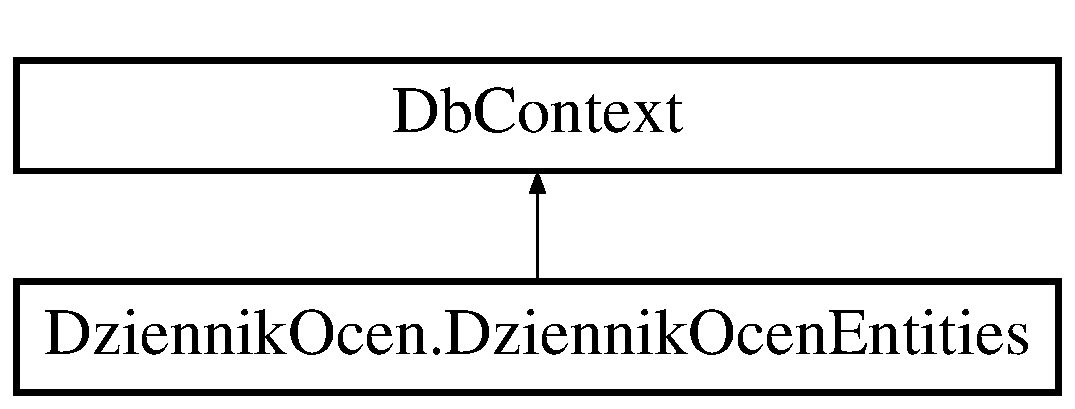
\includegraphics[height=2.000000cm]{class_dziennik_ocen_1_1_dziennik_ocen_entities}
\end{center}
\end{figure}
\subsection*{Public Member Functions}
\begin{DoxyCompactItemize}
\item 
\hyperlink{class_dziennik_ocen_1_1_dziennik_ocen_entities_ac3342686c2273ce2aa63726dd18c30de}{Dziennik\+Ocen\+Entities} ()
\item 
virtual int \hyperlink{class_dziennik_ocen_1_1_dziennik_ocen_entities_a1a8b451c6e153204c17b2e71110e8c34}{sp\+\_\+alterdiagram} (string diagramname, Nullable$<$ int $>$ owner\+\_\+id, Nullable$<$ int $>$ version, byte\mbox{[}$\,$\mbox{]} definition)
\item 
virtual int \hyperlink{class_dziennik_ocen_1_1_dziennik_ocen_entities_a044325cc04f005d56d4cf3d461ad2ee3}{sp\+\_\+creatediagram} (string diagramname, Nullable$<$ int $>$ owner\+\_\+id, Nullable$<$ int $>$ version, byte\mbox{[}$\,$\mbox{]} definition)
\item 
virtual int \hyperlink{class_dziennik_ocen_1_1_dziennik_ocen_entities_aef7fc0cd2e463ccf54e1967825e2c4f8}{sp\+\_\+dropdiagram} (string diagramname, Nullable$<$ int $>$ owner\+\_\+id)
\item 
virtual Object\+Result$<$ \hyperlink{class_dziennik_ocen_1_1sp__helpdiagramdefinition___result}{sp\+\_\+helpdiagramdefinition\+\_\+\+Result} $>$ \hyperlink{class_dziennik_ocen_1_1_dziennik_ocen_entities_a1a08762b12fdba65c46dc89808a036f2}{sp\+\_\+helpdiagramdefinition} (string diagramname, Nullable$<$ int $>$ owner\+\_\+id)
\item 
virtual Object\+Result$<$ \hyperlink{class_dziennik_ocen_1_1sp__helpdiagrams___result}{sp\+\_\+helpdiagrams\+\_\+\+Result} $>$ \hyperlink{class_dziennik_ocen_1_1_dziennik_ocen_entities_ae183901a590f1c4ac6925f9749881082}{sp\+\_\+helpdiagrams} (string diagramname, Nullable$<$ int $>$ owner\+\_\+id)
\item 
virtual int \hyperlink{class_dziennik_ocen_1_1_dziennik_ocen_entities_ab357421964b49d95a9410ccc0f381214}{sp\+\_\+renamediagram} (string diagramname, Nullable$<$ int $>$ owner\+\_\+id, string new\+\_\+diagramname)
\item 
virtual int \hyperlink{class_dziennik_ocen_1_1_dziennik_ocen_entities_a8bf06603c78ada012177682f17a8315d}{sp\+\_\+upgraddiagrams} ()
\end{DoxyCompactItemize}
\subsection*{Protected Member Functions}
\begin{DoxyCompactItemize}
\item 
override void \hyperlink{class_dziennik_ocen_1_1_dziennik_ocen_entities_a30945a5af85b1d25e95b6734a577df42}{On\+Model\+Creating} (Db\+Model\+Builder model\+Builder)
\end{DoxyCompactItemize}
\subsection*{Properties}
\begin{DoxyCompactItemize}
\item 
Db\+Set$<$ \hyperlink{class_dziennik_ocen_1_1_g_r_u_p_a}{G\+R\+U\+PA} $>$ \hyperlink{class_dziennik_ocen_1_1_dziennik_ocen_entities_ad4334a280ce27588b4e549d1f9bdf370}{G\+R\+U\+PA}\hspace{0.3cm}{\ttfamily  \mbox{[}get, set\mbox{]}}
\item 
Db\+Set$<$ \hyperlink{class_dziennik_ocen_1_1_p_r_o_j_e_k_t}{P\+R\+O\+J\+E\+KT} $>$ \hyperlink{class_dziennik_ocen_1_1_dziennik_ocen_entities_a4a2aa21f8f38da7c5964e8d0f104e93b}{P\+R\+O\+J\+E\+KT}\hspace{0.3cm}{\ttfamily  \mbox{[}get, set\mbox{]}}
\item 
Db\+Set$<$ \hyperlink{class_dziennik_ocen_1_1projekty}{projekty} $>$ \hyperlink{class_dziennik_ocen_1_1_dziennik_ocen_entities_aa5fb13b67d92101e714b25d03353a313}{projekty}\hspace{0.3cm}{\ttfamily  \mbox{[}get, set\mbox{]}}
\item 
Db\+Set$<$ \hyperlink{class_dziennik_ocen_1_1_p_r_o_w_a_d_z_xC4_x84_c_y}{P\+R\+O\+W\+A\+D\+ZĄ\+CY} $>$ \hyperlink{class_dziennik_ocen_1_1_dziennik_ocen_entities_a395e57706a24fe9f929e53dc41e73ea0}{P\+R\+O\+W\+A\+D\+ZĄ\+CY}\hspace{0.3cm}{\ttfamily  \mbox{[}get, set\mbox{]}}
\item 
Db\+Set$<$ \hyperlink{class_dziennik_ocen_1_1_p_r_z_e_d_m_i_o_t}{P\+R\+Z\+E\+D\+M\+I\+OT} $>$ \hyperlink{class_dziennik_ocen_1_1_dziennik_ocen_entities_a7e15ce866104268720701617a3f1ff7c}{P\+R\+Z\+E\+D\+M\+I\+OT}\hspace{0.3cm}{\ttfamily  \mbox{[}get, set\mbox{]}}
\item 
Db\+Set$<$ \hyperlink{class_dziennik_ocen_1_1przedmioty}{przedmioty} $>$ \hyperlink{class_dziennik_ocen_1_1_dziennik_ocen_entities_ae76bc2bdeec6f76972792082e1656298}{przedmioty}\hspace{0.3cm}{\ttfamily  \mbox{[}get, set\mbox{]}}
\item 
Db\+Set$<$ \hyperlink{class_dziennik_ocen_1_1_s_t_u_d_e_n_t}{S\+T\+U\+D\+E\+NT} $>$ \hyperlink{class_dziennik_ocen_1_1_dziennik_ocen_entities_a6551b0ae65432cd0d3db51f56fbeb36f}{S\+T\+U\+D\+E\+NT}\hspace{0.3cm}{\ttfamily  \mbox{[}get, set\mbox{]}}
\end{DoxyCompactItemize}


\subsection{Constructor \& Destructor Documentation}
\mbox{\Hypertarget{class_dziennik_ocen_1_1_dziennik_ocen_entities_ac3342686c2273ce2aa63726dd18c30de}\label{class_dziennik_ocen_1_1_dziennik_ocen_entities_ac3342686c2273ce2aa63726dd18c30de}} 
\index{Dziennik\+Ocen\+::\+Dziennik\+Ocen\+Entities@{Dziennik\+Ocen\+::\+Dziennik\+Ocen\+Entities}!Dziennik\+Ocen\+Entities@{Dziennik\+Ocen\+Entities}}
\index{Dziennik\+Ocen\+Entities@{Dziennik\+Ocen\+Entities}!Dziennik\+Ocen\+::\+Dziennik\+Ocen\+Entities@{Dziennik\+Ocen\+::\+Dziennik\+Ocen\+Entities}}
\subsubsection{\texorpdfstring{Dziennik\+Ocen\+Entities()}{DziennikOcenEntities()}}
{\footnotesize\ttfamily Dziennik\+Ocen.\+Dziennik\+Ocen\+Entities.\+Dziennik\+Ocen\+Entities (\begin{DoxyParamCaption}{ }\end{DoxyParamCaption})\hspace{0.3cm}{\ttfamily [inline]}}



\subsection{Member Function Documentation}
\mbox{\Hypertarget{class_dziennik_ocen_1_1_dziennik_ocen_entities_a30945a5af85b1d25e95b6734a577df42}\label{class_dziennik_ocen_1_1_dziennik_ocen_entities_a30945a5af85b1d25e95b6734a577df42}} 
\index{Dziennik\+Ocen\+::\+Dziennik\+Ocen\+Entities@{Dziennik\+Ocen\+::\+Dziennik\+Ocen\+Entities}!On\+Model\+Creating@{On\+Model\+Creating}}
\index{On\+Model\+Creating@{On\+Model\+Creating}!Dziennik\+Ocen\+::\+Dziennik\+Ocen\+Entities@{Dziennik\+Ocen\+::\+Dziennik\+Ocen\+Entities}}
\subsubsection{\texorpdfstring{On\+Model\+Creating()}{OnModelCreating()}}
{\footnotesize\ttfamily override void Dziennik\+Ocen.\+Dziennik\+Ocen\+Entities.\+On\+Model\+Creating (\begin{DoxyParamCaption}\item[{Db\+Model\+Builder}]{model\+Builder }\end{DoxyParamCaption})\hspace{0.3cm}{\ttfamily [inline]}, {\ttfamily [protected]}}

\mbox{\Hypertarget{class_dziennik_ocen_1_1_dziennik_ocen_entities_a1a8b451c6e153204c17b2e71110e8c34}\label{class_dziennik_ocen_1_1_dziennik_ocen_entities_a1a8b451c6e153204c17b2e71110e8c34}} 
\index{Dziennik\+Ocen\+::\+Dziennik\+Ocen\+Entities@{Dziennik\+Ocen\+::\+Dziennik\+Ocen\+Entities}!sp\+\_\+alterdiagram@{sp\+\_\+alterdiagram}}
\index{sp\+\_\+alterdiagram@{sp\+\_\+alterdiagram}!Dziennik\+Ocen\+::\+Dziennik\+Ocen\+Entities@{Dziennik\+Ocen\+::\+Dziennik\+Ocen\+Entities}}
\subsubsection{\texorpdfstring{sp\+\_\+alterdiagram()}{sp\_alterdiagram()}}
{\footnotesize\ttfamily virtual int Dziennik\+Ocen.\+Dziennik\+Ocen\+Entities.\+sp\+\_\+alterdiagram (\begin{DoxyParamCaption}\item[{string}]{diagramname,  }\item[{Nullable$<$ int $>$}]{owner\+\_\+id,  }\item[{Nullable$<$ int $>$}]{version,  }\item[{byte \mbox{[}$\,$\mbox{]}}]{definition }\end{DoxyParamCaption})\hspace{0.3cm}{\ttfamily [inline]}, {\ttfamily [virtual]}}

\mbox{\Hypertarget{class_dziennik_ocen_1_1_dziennik_ocen_entities_a044325cc04f005d56d4cf3d461ad2ee3}\label{class_dziennik_ocen_1_1_dziennik_ocen_entities_a044325cc04f005d56d4cf3d461ad2ee3}} 
\index{Dziennik\+Ocen\+::\+Dziennik\+Ocen\+Entities@{Dziennik\+Ocen\+::\+Dziennik\+Ocen\+Entities}!sp\+\_\+creatediagram@{sp\+\_\+creatediagram}}
\index{sp\+\_\+creatediagram@{sp\+\_\+creatediagram}!Dziennik\+Ocen\+::\+Dziennik\+Ocen\+Entities@{Dziennik\+Ocen\+::\+Dziennik\+Ocen\+Entities}}
\subsubsection{\texorpdfstring{sp\+\_\+creatediagram()}{sp\_creatediagram()}}
{\footnotesize\ttfamily virtual int Dziennik\+Ocen.\+Dziennik\+Ocen\+Entities.\+sp\+\_\+creatediagram (\begin{DoxyParamCaption}\item[{string}]{diagramname,  }\item[{Nullable$<$ int $>$}]{owner\+\_\+id,  }\item[{Nullable$<$ int $>$}]{version,  }\item[{byte \mbox{[}$\,$\mbox{]}}]{definition }\end{DoxyParamCaption})\hspace{0.3cm}{\ttfamily [inline]}, {\ttfamily [virtual]}}

\mbox{\Hypertarget{class_dziennik_ocen_1_1_dziennik_ocen_entities_aef7fc0cd2e463ccf54e1967825e2c4f8}\label{class_dziennik_ocen_1_1_dziennik_ocen_entities_aef7fc0cd2e463ccf54e1967825e2c4f8}} 
\index{Dziennik\+Ocen\+::\+Dziennik\+Ocen\+Entities@{Dziennik\+Ocen\+::\+Dziennik\+Ocen\+Entities}!sp\+\_\+dropdiagram@{sp\+\_\+dropdiagram}}
\index{sp\+\_\+dropdiagram@{sp\+\_\+dropdiagram}!Dziennik\+Ocen\+::\+Dziennik\+Ocen\+Entities@{Dziennik\+Ocen\+::\+Dziennik\+Ocen\+Entities}}
\subsubsection{\texorpdfstring{sp\+\_\+dropdiagram()}{sp\_dropdiagram()}}
{\footnotesize\ttfamily virtual int Dziennik\+Ocen.\+Dziennik\+Ocen\+Entities.\+sp\+\_\+dropdiagram (\begin{DoxyParamCaption}\item[{string}]{diagramname,  }\item[{Nullable$<$ int $>$}]{owner\+\_\+id }\end{DoxyParamCaption})\hspace{0.3cm}{\ttfamily [inline]}, {\ttfamily [virtual]}}

\mbox{\Hypertarget{class_dziennik_ocen_1_1_dziennik_ocen_entities_a1a08762b12fdba65c46dc89808a036f2}\label{class_dziennik_ocen_1_1_dziennik_ocen_entities_a1a08762b12fdba65c46dc89808a036f2}} 
\index{Dziennik\+Ocen\+::\+Dziennik\+Ocen\+Entities@{Dziennik\+Ocen\+::\+Dziennik\+Ocen\+Entities}!sp\+\_\+helpdiagramdefinition@{sp\+\_\+helpdiagramdefinition}}
\index{sp\+\_\+helpdiagramdefinition@{sp\+\_\+helpdiagramdefinition}!Dziennik\+Ocen\+::\+Dziennik\+Ocen\+Entities@{Dziennik\+Ocen\+::\+Dziennik\+Ocen\+Entities}}
\subsubsection{\texorpdfstring{sp\+\_\+helpdiagramdefinition()}{sp\_helpdiagramdefinition()}}
{\footnotesize\ttfamily virtual Object\+Result$<$\hyperlink{class_dziennik_ocen_1_1sp__helpdiagramdefinition___result}{sp\+\_\+helpdiagramdefinition\+\_\+\+Result}$>$ Dziennik\+Ocen.\+Dziennik\+Ocen\+Entities.\+sp\+\_\+helpdiagramdefinition (\begin{DoxyParamCaption}\item[{string}]{diagramname,  }\item[{Nullable$<$ int $>$}]{owner\+\_\+id }\end{DoxyParamCaption})\hspace{0.3cm}{\ttfamily [inline]}, {\ttfamily [virtual]}}

\mbox{\Hypertarget{class_dziennik_ocen_1_1_dziennik_ocen_entities_ae183901a590f1c4ac6925f9749881082}\label{class_dziennik_ocen_1_1_dziennik_ocen_entities_ae183901a590f1c4ac6925f9749881082}} 
\index{Dziennik\+Ocen\+::\+Dziennik\+Ocen\+Entities@{Dziennik\+Ocen\+::\+Dziennik\+Ocen\+Entities}!sp\+\_\+helpdiagrams@{sp\+\_\+helpdiagrams}}
\index{sp\+\_\+helpdiagrams@{sp\+\_\+helpdiagrams}!Dziennik\+Ocen\+::\+Dziennik\+Ocen\+Entities@{Dziennik\+Ocen\+::\+Dziennik\+Ocen\+Entities}}
\subsubsection{\texorpdfstring{sp\+\_\+helpdiagrams()}{sp\_helpdiagrams()}}
{\footnotesize\ttfamily virtual Object\+Result$<$\hyperlink{class_dziennik_ocen_1_1sp__helpdiagrams___result}{sp\+\_\+helpdiagrams\+\_\+\+Result}$>$ Dziennik\+Ocen.\+Dziennik\+Ocen\+Entities.\+sp\+\_\+helpdiagrams (\begin{DoxyParamCaption}\item[{string}]{diagramname,  }\item[{Nullable$<$ int $>$}]{owner\+\_\+id }\end{DoxyParamCaption})\hspace{0.3cm}{\ttfamily [inline]}, {\ttfamily [virtual]}}

\mbox{\Hypertarget{class_dziennik_ocen_1_1_dziennik_ocen_entities_ab357421964b49d95a9410ccc0f381214}\label{class_dziennik_ocen_1_1_dziennik_ocen_entities_ab357421964b49d95a9410ccc0f381214}} 
\index{Dziennik\+Ocen\+::\+Dziennik\+Ocen\+Entities@{Dziennik\+Ocen\+::\+Dziennik\+Ocen\+Entities}!sp\+\_\+renamediagram@{sp\+\_\+renamediagram}}
\index{sp\+\_\+renamediagram@{sp\+\_\+renamediagram}!Dziennik\+Ocen\+::\+Dziennik\+Ocen\+Entities@{Dziennik\+Ocen\+::\+Dziennik\+Ocen\+Entities}}
\subsubsection{\texorpdfstring{sp\+\_\+renamediagram()}{sp\_renamediagram()}}
{\footnotesize\ttfamily virtual int Dziennik\+Ocen.\+Dziennik\+Ocen\+Entities.\+sp\+\_\+renamediagram (\begin{DoxyParamCaption}\item[{string}]{diagramname,  }\item[{Nullable$<$ int $>$}]{owner\+\_\+id,  }\item[{string}]{new\+\_\+diagramname }\end{DoxyParamCaption})\hspace{0.3cm}{\ttfamily [inline]}, {\ttfamily [virtual]}}

\mbox{\Hypertarget{class_dziennik_ocen_1_1_dziennik_ocen_entities_a8bf06603c78ada012177682f17a8315d}\label{class_dziennik_ocen_1_1_dziennik_ocen_entities_a8bf06603c78ada012177682f17a8315d}} 
\index{Dziennik\+Ocen\+::\+Dziennik\+Ocen\+Entities@{Dziennik\+Ocen\+::\+Dziennik\+Ocen\+Entities}!sp\+\_\+upgraddiagrams@{sp\+\_\+upgraddiagrams}}
\index{sp\+\_\+upgraddiagrams@{sp\+\_\+upgraddiagrams}!Dziennik\+Ocen\+::\+Dziennik\+Ocen\+Entities@{Dziennik\+Ocen\+::\+Dziennik\+Ocen\+Entities}}
\subsubsection{\texorpdfstring{sp\+\_\+upgraddiagrams()}{sp\_upgraddiagrams()}}
{\footnotesize\ttfamily virtual int Dziennik\+Ocen.\+Dziennik\+Ocen\+Entities.\+sp\+\_\+upgraddiagrams (\begin{DoxyParamCaption}{ }\end{DoxyParamCaption})\hspace{0.3cm}{\ttfamily [inline]}, {\ttfamily [virtual]}}



\subsection{Property Documentation}
\mbox{\Hypertarget{class_dziennik_ocen_1_1_dziennik_ocen_entities_ad4334a280ce27588b4e549d1f9bdf370}\label{class_dziennik_ocen_1_1_dziennik_ocen_entities_ad4334a280ce27588b4e549d1f9bdf370}} 
\index{Dziennik\+Ocen\+::\+Dziennik\+Ocen\+Entities@{Dziennik\+Ocen\+::\+Dziennik\+Ocen\+Entities}!G\+R\+U\+PA@{G\+R\+U\+PA}}
\index{G\+R\+U\+PA@{G\+R\+U\+PA}!Dziennik\+Ocen\+::\+Dziennik\+Ocen\+Entities@{Dziennik\+Ocen\+::\+Dziennik\+Ocen\+Entities}}
\subsubsection{\texorpdfstring{G\+R\+U\+PA}{GRUPA}}
{\footnotesize\ttfamily Db\+Set$<$\hyperlink{class_dziennik_ocen_1_1_g_r_u_p_a}{G\+R\+U\+PA}$>$ Dziennik\+Ocen.\+Dziennik\+Ocen\+Entities.\+G\+R\+U\+PA\hspace{0.3cm}{\ttfamily [get]}, {\ttfamily [set]}}

\mbox{\Hypertarget{class_dziennik_ocen_1_1_dziennik_ocen_entities_a4a2aa21f8f38da7c5964e8d0f104e93b}\label{class_dziennik_ocen_1_1_dziennik_ocen_entities_a4a2aa21f8f38da7c5964e8d0f104e93b}} 
\index{Dziennik\+Ocen\+::\+Dziennik\+Ocen\+Entities@{Dziennik\+Ocen\+::\+Dziennik\+Ocen\+Entities}!P\+R\+O\+J\+E\+KT@{P\+R\+O\+J\+E\+KT}}
\index{P\+R\+O\+J\+E\+KT@{P\+R\+O\+J\+E\+KT}!Dziennik\+Ocen\+::\+Dziennik\+Ocen\+Entities@{Dziennik\+Ocen\+::\+Dziennik\+Ocen\+Entities}}
\subsubsection{\texorpdfstring{P\+R\+O\+J\+E\+KT}{PROJEKT}}
{\footnotesize\ttfamily Db\+Set$<$\hyperlink{class_dziennik_ocen_1_1_p_r_o_j_e_k_t}{P\+R\+O\+J\+E\+KT}$>$ Dziennik\+Ocen.\+Dziennik\+Ocen\+Entities.\+P\+R\+O\+J\+E\+KT\hspace{0.3cm}{\ttfamily [get]}, {\ttfamily [set]}}

\mbox{\Hypertarget{class_dziennik_ocen_1_1_dziennik_ocen_entities_aa5fb13b67d92101e714b25d03353a313}\label{class_dziennik_ocen_1_1_dziennik_ocen_entities_aa5fb13b67d92101e714b25d03353a313}} 
\index{Dziennik\+Ocen\+::\+Dziennik\+Ocen\+Entities@{Dziennik\+Ocen\+::\+Dziennik\+Ocen\+Entities}!projekty@{projekty}}
\index{projekty@{projekty}!Dziennik\+Ocen\+::\+Dziennik\+Ocen\+Entities@{Dziennik\+Ocen\+::\+Dziennik\+Ocen\+Entities}}
\subsubsection{\texorpdfstring{projekty}{projekty}}
{\footnotesize\ttfamily Db\+Set$<$\hyperlink{class_dziennik_ocen_1_1projekty}{projekty}$>$ Dziennik\+Ocen.\+Dziennik\+Ocen\+Entities.\+projekty\hspace{0.3cm}{\ttfamily [get]}, {\ttfamily [set]}}

\mbox{\Hypertarget{class_dziennik_ocen_1_1_dziennik_ocen_entities_a395e57706a24fe9f929e53dc41e73ea0}\label{class_dziennik_ocen_1_1_dziennik_ocen_entities_a395e57706a24fe9f929e53dc41e73ea0}} 
\index{Dziennik\+Ocen\+::\+Dziennik\+Ocen\+Entities@{Dziennik\+Ocen\+::\+Dziennik\+Ocen\+Entities}!P\+R\+O\+W\+A\+D\+ZĄ\+CY@{P\+R\+O\+W\+A\+D\+ZĄ\+CY}}
\index{P\+R\+O\+W\+A\+D\+ZĄ\+CY@{P\+R\+O\+W\+A\+D\+ZĄ\+CY}!Dziennik\+Ocen\+::\+Dziennik\+Ocen\+Entities@{Dziennik\+Ocen\+::\+Dziennik\+Ocen\+Entities}}
\subsubsection{\texorpdfstring{P\+R\+O\+W\+A\+D\+ZĄ\+CY}{PROWADZĄCY}}
{\footnotesize\ttfamily Db\+Set$<$\hyperlink{class_dziennik_ocen_1_1_p_r_o_w_a_d_z_xC4_x84_c_y}{P\+R\+O\+W\+A\+D\+ZĄ\+CY}$>$ Dziennik\+Ocen.\+Dziennik\+Ocen\+Entities.\+P\+R\+O\+W\+A\+D\+ZĄ\+CY\hspace{0.3cm}{\ttfamily [get]}, {\ttfamily [set]}}

\mbox{\Hypertarget{class_dziennik_ocen_1_1_dziennik_ocen_entities_a7e15ce866104268720701617a3f1ff7c}\label{class_dziennik_ocen_1_1_dziennik_ocen_entities_a7e15ce866104268720701617a3f1ff7c}} 
\index{Dziennik\+Ocen\+::\+Dziennik\+Ocen\+Entities@{Dziennik\+Ocen\+::\+Dziennik\+Ocen\+Entities}!P\+R\+Z\+E\+D\+M\+I\+OT@{P\+R\+Z\+E\+D\+M\+I\+OT}}
\index{P\+R\+Z\+E\+D\+M\+I\+OT@{P\+R\+Z\+E\+D\+M\+I\+OT}!Dziennik\+Ocen\+::\+Dziennik\+Ocen\+Entities@{Dziennik\+Ocen\+::\+Dziennik\+Ocen\+Entities}}
\subsubsection{\texorpdfstring{P\+R\+Z\+E\+D\+M\+I\+OT}{PRZEDMIOT}}
{\footnotesize\ttfamily Db\+Set$<$\hyperlink{class_dziennik_ocen_1_1_p_r_z_e_d_m_i_o_t}{P\+R\+Z\+E\+D\+M\+I\+OT}$>$ Dziennik\+Ocen.\+Dziennik\+Ocen\+Entities.\+P\+R\+Z\+E\+D\+M\+I\+OT\hspace{0.3cm}{\ttfamily [get]}, {\ttfamily [set]}}

\mbox{\Hypertarget{class_dziennik_ocen_1_1_dziennik_ocen_entities_ae76bc2bdeec6f76972792082e1656298}\label{class_dziennik_ocen_1_1_dziennik_ocen_entities_ae76bc2bdeec6f76972792082e1656298}} 
\index{Dziennik\+Ocen\+::\+Dziennik\+Ocen\+Entities@{Dziennik\+Ocen\+::\+Dziennik\+Ocen\+Entities}!przedmioty@{przedmioty}}
\index{przedmioty@{przedmioty}!Dziennik\+Ocen\+::\+Dziennik\+Ocen\+Entities@{Dziennik\+Ocen\+::\+Dziennik\+Ocen\+Entities}}
\subsubsection{\texorpdfstring{przedmioty}{przedmioty}}
{\footnotesize\ttfamily Db\+Set$<$\hyperlink{class_dziennik_ocen_1_1przedmioty}{przedmioty}$>$ Dziennik\+Ocen.\+Dziennik\+Ocen\+Entities.\+przedmioty\hspace{0.3cm}{\ttfamily [get]}, {\ttfamily [set]}}

\mbox{\Hypertarget{class_dziennik_ocen_1_1_dziennik_ocen_entities_a6551b0ae65432cd0d3db51f56fbeb36f}\label{class_dziennik_ocen_1_1_dziennik_ocen_entities_a6551b0ae65432cd0d3db51f56fbeb36f}} 
\index{Dziennik\+Ocen\+::\+Dziennik\+Ocen\+Entities@{Dziennik\+Ocen\+::\+Dziennik\+Ocen\+Entities}!S\+T\+U\+D\+E\+NT@{S\+T\+U\+D\+E\+NT}}
\index{S\+T\+U\+D\+E\+NT@{S\+T\+U\+D\+E\+NT}!Dziennik\+Ocen\+::\+Dziennik\+Ocen\+Entities@{Dziennik\+Ocen\+::\+Dziennik\+Ocen\+Entities}}
\subsubsection{\texorpdfstring{S\+T\+U\+D\+E\+NT}{STUDENT}}
{\footnotesize\ttfamily Db\+Set$<$\hyperlink{class_dziennik_ocen_1_1_s_t_u_d_e_n_t}{S\+T\+U\+D\+E\+NT}$>$ Dziennik\+Ocen.\+Dziennik\+Ocen\+Entities.\+S\+T\+U\+D\+E\+NT\hspace{0.3cm}{\ttfamily [get]}, {\ttfamily [set]}}



The documentation for this class was generated from the following file\+:\begin{DoxyCompactItemize}
\item 
Dziennik\+Ocen/\hyperlink{_dziennik_ocen_8_context_8cs}{Dziennik\+Ocen.\+Context.\+cs}\end{DoxyCompactItemize}

\hypertarget{class_dziennik_ocen_1_1_form1}{}\section{Dziennik\+Ocen.\+Form1 Class Reference}
\label{class_dziennik_ocen_1_1_form1}\index{Dziennik\+Ocen.\+Form1@{Dziennik\+Ocen.\+Form1}}
Inheritance diagram for Dziennik\+Ocen.\+Form1\+:\begin{figure}[H]
\begin{center}
\leavevmode
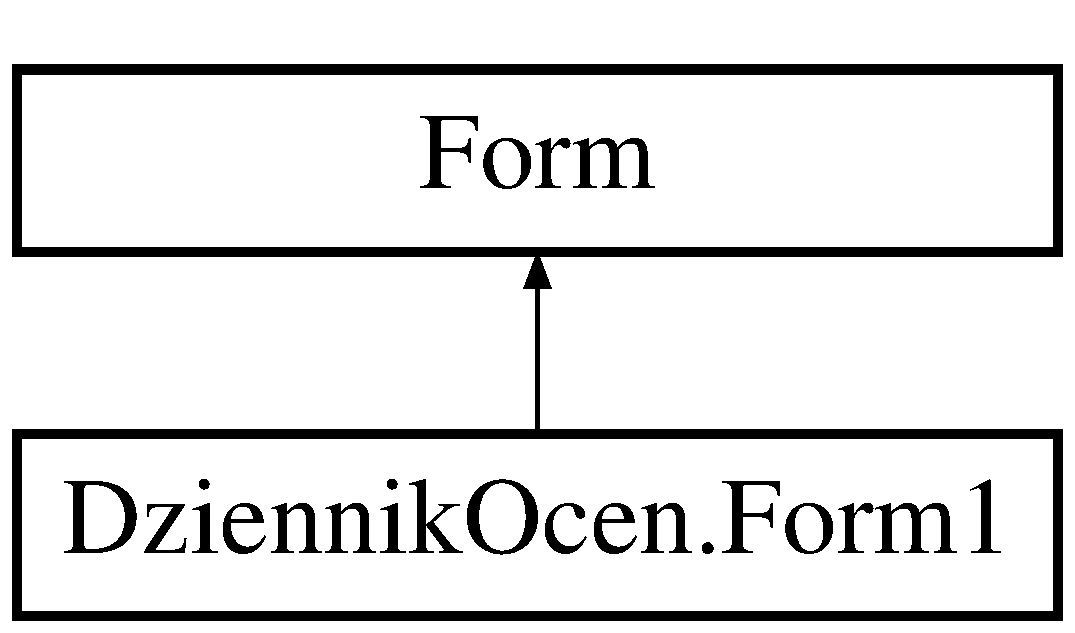
\includegraphics[height=2.000000cm]{class_dziennik_ocen_1_1_form1}
\end{center}
\end{figure}
\subsection*{Public Member Functions}
\begin{DoxyCompactItemize}
\item 
\hyperlink{class_dziennik_ocen_1_1_form1_a494b133ac4b159fcfc42561ce2c72002}{Form1} ()
\end{DoxyCompactItemize}
\subsection*{Protected Member Functions}
\begin{DoxyCompactItemize}
\item 
override void \hyperlink{class_dziennik_ocen_1_1_form1_a64a7924e831567e78bb499a6baa0e543}{Dispose} (bool disposing)
\begin{DoxyCompactList}\small\item\em Clean up any resources being used. \end{DoxyCompactList}\end{DoxyCompactItemize}
\subsection*{Private Member Functions}
\begin{DoxyCompactItemize}
\item 
void \hyperlink{class_dziennik_ocen_1_1_form1_a28adc07ca2d4d960f57b60cae2b1bad9}{btn\+Zaloguj\+\_\+\+Click} (object sender, Event\+Args e)
\item 
void \hyperlink{class_dziennik_ocen_1_1_form1_acb939aa086bb943e9720d95d9142ef88}{btn\+Student\+\_\+\+Click} (object sender, Event\+Args e)
\item 
void \hyperlink{class_dziennik_ocen_1_1_form1_a0b2d561130044c417c0c5d0e7d4172b9}{btn\+Prowadzacy\+\_\+\+Click} (object sender, Event\+Args e)
\item 
void \hyperlink{class_dziennik_ocen_1_1_form1_a600f65aebd5840bfccaf74538a7259a0}{btn\+Administrator\+\_\+\+Click} (object sender, Event\+Args e)
\item 
void \hyperlink{class_dziennik_ocen_1_1_form1_a25d1f1865febb87fc9186127ca72793c}{Initialize\+Component} ()
\begin{DoxyCompactList}\small\item\em Required method for Designer support -\/ do not modify the contents of this method with the code editor. \end{DoxyCompactList}\end{DoxyCompactItemize}
\subsection*{Private Attributes}
\begin{DoxyCompactItemize}
\item 
\hyperlink{class_dziennik_ocen_1_1_dziennik_ocen_entities}{Dziennik\+Ocen\+Entities} \hyperlink{class_dziennik_ocen_1_1_form1_aeeaa17c2c70a1daae0e6f26f1fc788e6}{db} = new \hyperlink{class_dziennik_ocen_1_1_dziennik_ocen_entities}{Dziennik\+Ocen\+Entities}()
\item 
System.\+Component\+Model.\+I\+Container \hyperlink{class_dziennik_ocen_1_1_form1_a7b1d7b5c990e5a9bc92a1755cb4b5b58}{components} = null
\begin{DoxyCompactList}\small\item\em Required designer variable. \end{DoxyCompactList}\item 
System.\+Windows.\+Forms.\+Label \hyperlink{class_dziennik_ocen_1_1_form1_a21e8417347f7fbada2f5b5f5cde8c581}{lbl\+Logowanie}
\item 
System.\+Windows.\+Forms.\+Text\+Box \hyperlink{class_dziennik_ocen_1_1_form1_ac97730ed2eab3b9713c73112dc7417fb}{tbx\+Email}
\item 
System.\+Windows.\+Forms.\+Text\+Box \hyperlink{class_dziennik_ocen_1_1_form1_ae78ef2ccf550d5af060ea54cbc28077f}{tbx\+Haslo}
\item 
System.\+Windows.\+Forms.\+Label \hyperlink{class_dziennik_ocen_1_1_form1_ab1781ae675111e00fea84baf36b09b30}{label1}
\item 
System.\+Windows.\+Forms.\+Label \hyperlink{class_dziennik_ocen_1_1_form1_a3c5bd2259bef1a618510464d4377862d}{label2}
\item 
System.\+Windows.\+Forms.\+Button \hyperlink{class_dziennik_ocen_1_1_form1_aac2dedd2aeda7358bf65c5ed7a518ff3}{btn\+Zaloguj}
\item 
System.\+Windows.\+Forms.\+Label \hyperlink{class_dziennik_ocen_1_1_form1_a8bc43c594a39bdb51bb665861a585c6b}{label3}
\item 
System.\+Windows.\+Forms.\+Button \hyperlink{class_dziennik_ocen_1_1_form1_ad351dcf0c98815603b220c185d0f743d}{btn\+Student}
\item 
System.\+Windows.\+Forms.\+Button \hyperlink{class_dziennik_ocen_1_1_form1_a3e80414e3a1d2c92f9649e57e4c610a8}{btn\+Prowadzacy}
\item 
System.\+Windows.\+Forms.\+Button \hyperlink{class_dziennik_ocen_1_1_form1_a1bc9483c61d99951b6f2d57d24b4fe60}{btn\+Administrator}
\end{DoxyCompactItemize}


\subsection{Constructor \& Destructor Documentation}
\mbox{\Hypertarget{class_dziennik_ocen_1_1_form1_a494b133ac4b159fcfc42561ce2c72002}\label{class_dziennik_ocen_1_1_form1_a494b133ac4b159fcfc42561ce2c72002}} 
\index{Dziennik\+Ocen\+::\+Form1@{Dziennik\+Ocen\+::\+Form1}!Form1@{Form1}}
\index{Form1@{Form1}!Dziennik\+Ocen\+::\+Form1@{Dziennik\+Ocen\+::\+Form1}}
\subsubsection{\texorpdfstring{Form1()}{Form1()}}
{\footnotesize\ttfamily Dziennik\+Ocen.\+Form1.\+Form1 (\begin{DoxyParamCaption}{ }\end{DoxyParamCaption})\hspace{0.3cm}{\ttfamily [inline]}}



\subsection{Member Function Documentation}
\mbox{\Hypertarget{class_dziennik_ocen_1_1_form1_a600f65aebd5840bfccaf74538a7259a0}\label{class_dziennik_ocen_1_1_form1_a600f65aebd5840bfccaf74538a7259a0}} 
\index{Dziennik\+Ocen\+::\+Form1@{Dziennik\+Ocen\+::\+Form1}!btn\+Administrator\+\_\+\+Click@{btn\+Administrator\+\_\+\+Click}}
\index{btn\+Administrator\+\_\+\+Click@{btn\+Administrator\+\_\+\+Click}!Dziennik\+Ocen\+::\+Form1@{Dziennik\+Ocen\+::\+Form1}}
\subsubsection{\texorpdfstring{btn\+Administrator\+\_\+\+Click()}{btnAdministrator\_Click()}}
{\footnotesize\ttfamily void Dziennik\+Ocen.\+Form1.\+btn\+Administrator\+\_\+\+Click (\begin{DoxyParamCaption}\item[{object}]{sender,  }\item[{Event\+Args}]{e }\end{DoxyParamCaption})\hspace{0.3cm}{\ttfamily [inline]}, {\ttfamily [private]}}

\mbox{\Hypertarget{class_dziennik_ocen_1_1_form1_a0b2d561130044c417c0c5d0e7d4172b9}\label{class_dziennik_ocen_1_1_form1_a0b2d561130044c417c0c5d0e7d4172b9}} 
\index{Dziennik\+Ocen\+::\+Form1@{Dziennik\+Ocen\+::\+Form1}!btn\+Prowadzacy\+\_\+\+Click@{btn\+Prowadzacy\+\_\+\+Click}}
\index{btn\+Prowadzacy\+\_\+\+Click@{btn\+Prowadzacy\+\_\+\+Click}!Dziennik\+Ocen\+::\+Form1@{Dziennik\+Ocen\+::\+Form1}}
\subsubsection{\texorpdfstring{btn\+Prowadzacy\+\_\+\+Click()}{btnProwadzacy\_Click()}}
{\footnotesize\ttfamily void Dziennik\+Ocen.\+Form1.\+btn\+Prowadzacy\+\_\+\+Click (\begin{DoxyParamCaption}\item[{object}]{sender,  }\item[{Event\+Args}]{e }\end{DoxyParamCaption})\hspace{0.3cm}{\ttfamily [inline]}, {\ttfamily [private]}}

\mbox{\Hypertarget{class_dziennik_ocen_1_1_form1_acb939aa086bb943e9720d95d9142ef88}\label{class_dziennik_ocen_1_1_form1_acb939aa086bb943e9720d95d9142ef88}} 
\index{Dziennik\+Ocen\+::\+Form1@{Dziennik\+Ocen\+::\+Form1}!btn\+Student\+\_\+\+Click@{btn\+Student\+\_\+\+Click}}
\index{btn\+Student\+\_\+\+Click@{btn\+Student\+\_\+\+Click}!Dziennik\+Ocen\+::\+Form1@{Dziennik\+Ocen\+::\+Form1}}
\subsubsection{\texorpdfstring{btn\+Student\+\_\+\+Click()}{btnStudent\_Click()}}
{\footnotesize\ttfamily void Dziennik\+Ocen.\+Form1.\+btn\+Student\+\_\+\+Click (\begin{DoxyParamCaption}\item[{object}]{sender,  }\item[{Event\+Args}]{e }\end{DoxyParamCaption})\hspace{0.3cm}{\ttfamily [inline]}, {\ttfamily [private]}}

\mbox{\Hypertarget{class_dziennik_ocen_1_1_form1_a28adc07ca2d4d960f57b60cae2b1bad9}\label{class_dziennik_ocen_1_1_form1_a28adc07ca2d4d960f57b60cae2b1bad9}} 
\index{Dziennik\+Ocen\+::\+Form1@{Dziennik\+Ocen\+::\+Form1}!btn\+Zaloguj\+\_\+\+Click@{btn\+Zaloguj\+\_\+\+Click}}
\index{btn\+Zaloguj\+\_\+\+Click@{btn\+Zaloguj\+\_\+\+Click}!Dziennik\+Ocen\+::\+Form1@{Dziennik\+Ocen\+::\+Form1}}
\subsubsection{\texorpdfstring{btn\+Zaloguj\+\_\+\+Click()}{btnZaloguj\_Click()}}
{\footnotesize\ttfamily void Dziennik\+Ocen.\+Form1.\+btn\+Zaloguj\+\_\+\+Click (\begin{DoxyParamCaption}\item[{object}]{sender,  }\item[{Event\+Args}]{e }\end{DoxyParamCaption})\hspace{0.3cm}{\ttfamily [inline]}, {\ttfamily [private]}}

\mbox{\Hypertarget{class_dziennik_ocen_1_1_form1_a64a7924e831567e78bb499a6baa0e543}\label{class_dziennik_ocen_1_1_form1_a64a7924e831567e78bb499a6baa0e543}} 
\index{Dziennik\+Ocen\+::\+Form1@{Dziennik\+Ocen\+::\+Form1}!Dispose@{Dispose}}
\index{Dispose@{Dispose}!Dziennik\+Ocen\+::\+Form1@{Dziennik\+Ocen\+::\+Form1}}
\subsubsection{\texorpdfstring{Dispose()}{Dispose()}}
{\footnotesize\ttfamily override void Dziennik\+Ocen.\+Form1.\+Dispose (\begin{DoxyParamCaption}\item[{bool}]{disposing }\end{DoxyParamCaption})\hspace{0.3cm}{\ttfamily [inline]}, {\ttfamily [protected]}}



Clean up any resources being used. 


\begin{DoxyParams}{Parameters}
{\em disposing} & true if managed resources should be disposed; otherwise, false.\\
\hline
\end{DoxyParams}
\mbox{\Hypertarget{class_dziennik_ocen_1_1_form1_a25d1f1865febb87fc9186127ca72793c}\label{class_dziennik_ocen_1_1_form1_a25d1f1865febb87fc9186127ca72793c}} 
\index{Dziennik\+Ocen\+::\+Form1@{Dziennik\+Ocen\+::\+Form1}!Initialize\+Component@{Initialize\+Component}}
\index{Initialize\+Component@{Initialize\+Component}!Dziennik\+Ocen\+::\+Form1@{Dziennik\+Ocen\+::\+Form1}}
\subsubsection{\texorpdfstring{Initialize\+Component()}{InitializeComponent()}}
{\footnotesize\ttfamily void Dziennik\+Ocen.\+Form1.\+Initialize\+Component (\begin{DoxyParamCaption}{ }\end{DoxyParamCaption})\hspace{0.3cm}{\ttfamily [inline]}, {\ttfamily [private]}}



Required method for Designer support -\/ do not modify the contents of this method with the code editor. 



\subsection{Member Data Documentation}
\mbox{\Hypertarget{class_dziennik_ocen_1_1_form1_a1bc9483c61d99951b6f2d57d24b4fe60}\label{class_dziennik_ocen_1_1_form1_a1bc9483c61d99951b6f2d57d24b4fe60}} 
\index{Dziennik\+Ocen\+::\+Form1@{Dziennik\+Ocen\+::\+Form1}!btn\+Administrator@{btn\+Administrator}}
\index{btn\+Administrator@{btn\+Administrator}!Dziennik\+Ocen\+::\+Form1@{Dziennik\+Ocen\+::\+Form1}}
\subsubsection{\texorpdfstring{btn\+Administrator}{btnAdministrator}}
{\footnotesize\ttfamily System.\+Windows.\+Forms.\+Button Dziennik\+Ocen.\+Form1.\+btn\+Administrator\hspace{0.3cm}{\ttfamily [private]}}

\mbox{\Hypertarget{class_dziennik_ocen_1_1_form1_a3e80414e3a1d2c92f9649e57e4c610a8}\label{class_dziennik_ocen_1_1_form1_a3e80414e3a1d2c92f9649e57e4c610a8}} 
\index{Dziennik\+Ocen\+::\+Form1@{Dziennik\+Ocen\+::\+Form1}!btn\+Prowadzacy@{btn\+Prowadzacy}}
\index{btn\+Prowadzacy@{btn\+Prowadzacy}!Dziennik\+Ocen\+::\+Form1@{Dziennik\+Ocen\+::\+Form1}}
\subsubsection{\texorpdfstring{btn\+Prowadzacy}{btnProwadzacy}}
{\footnotesize\ttfamily System.\+Windows.\+Forms.\+Button Dziennik\+Ocen.\+Form1.\+btn\+Prowadzacy\hspace{0.3cm}{\ttfamily [private]}}

\mbox{\Hypertarget{class_dziennik_ocen_1_1_form1_ad351dcf0c98815603b220c185d0f743d}\label{class_dziennik_ocen_1_1_form1_ad351dcf0c98815603b220c185d0f743d}} 
\index{Dziennik\+Ocen\+::\+Form1@{Dziennik\+Ocen\+::\+Form1}!btn\+Student@{btn\+Student}}
\index{btn\+Student@{btn\+Student}!Dziennik\+Ocen\+::\+Form1@{Dziennik\+Ocen\+::\+Form1}}
\subsubsection{\texorpdfstring{btn\+Student}{btnStudent}}
{\footnotesize\ttfamily System.\+Windows.\+Forms.\+Button Dziennik\+Ocen.\+Form1.\+btn\+Student\hspace{0.3cm}{\ttfamily [private]}}

\mbox{\Hypertarget{class_dziennik_ocen_1_1_form1_aac2dedd2aeda7358bf65c5ed7a518ff3}\label{class_dziennik_ocen_1_1_form1_aac2dedd2aeda7358bf65c5ed7a518ff3}} 
\index{Dziennik\+Ocen\+::\+Form1@{Dziennik\+Ocen\+::\+Form1}!btn\+Zaloguj@{btn\+Zaloguj}}
\index{btn\+Zaloguj@{btn\+Zaloguj}!Dziennik\+Ocen\+::\+Form1@{Dziennik\+Ocen\+::\+Form1}}
\subsubsection{\texorpdfstring{btn\+Zaloguj}{btnZaloguj}}
{\footnotesize\ttfamily System.\+Windows.\+Forms.\+Button Dziennik\+Ocen.\+Form1.\+btn\+Zaloguj\hspace{0.3cm}{\ttfamily [private]}}

\mbox{\Hypertarget{class_dziennik_ocen_1_1_form1_a7b1d7b5c990e5a9bc92a1755cb4b5b58}\label{class_dziennik_ocen_1_1_form1_a7b1d7b5c990e5a9bc92a1755cb4b5b58}} 
\index{Dziennik\+Ocen\+::\+Form1@{Dziennik\+Ocen\+::\+Form1}!components@{components}}
\index{components@{components}!Dziennik\+Ocen\+::\+Form1@{Dziennik\+Ocen\+::\+Form1}}
\subsubsection{\texorpdfstring{components}{components}}
{\footnotesize\ttfamily System.\+Component\+Model.\+I\+Container Dziennik\+Ocen.\+Form1.\+components = null\hspace{0.3cm}{\ttfamily [private]}}



Required designer variable. 

\mbox{\Hypertarget{class_dziennik_ocen_1_1_form1_aeeaa17c2c70a1daae0e6f26f1fc788e6}\label{class_dziennik_ocen_1_1_form1_aeeaa17c2c70a1daae0e6f26f1fc788e6}} 
\index{Dziennik\+Ocen\+::\+Form1@{Dziennik\+Ocen\+::\+Form1}!db@{db}}
\index{db@{db}!Dziennik\+Ocen\+::\+Form1@{Dziennik\+Ocen\+::\+Form1}}
\subsubsection{\texorpdfstring{db}{db}}
{\footnotesize\ttfamily \hyperlink{class_dziennik_ocen_1_1_dziennik_ocen_entities}{Dziennik\+Ocen\+Entities} Dziennik\+Ocen.\+Form1.\+db = new \hyperlink{class_dziennik_ocen_1_1_dziennik_ocen_entities}{Dziennik\+Ocen\+Entities}()\hspace{0.3cm}{\ttfamily [private]}}

\mbox{\Hypertarget{class_dziennik_ocen_1_1_form1_ab1781ae675111e00fea84baf36b09b30}\label{class_dziennik_ocen_1_1_form1_ab1781ae675111e00fea84baf36b09b30}} 
\index{Dziennik\+Ocen\+::\+Form1@{Dziennik\+Ocen\+::\+Form1}!label1@{label1}}
\index{label1@{label1}!Dziennik\+Ocen\+::\+Form1@{Dziennik\+Ocen\+::\+Form1}}
\subsubsection{\texorpdfstring{label1}{label1}}
{\footnotesize\ttfamily System.\+Windows.\+Forms.\+Label Dziennik\+Ocen.\+Form1.\+label1\hspace{0.3cm}{\ttfamily [private]}}

\mbox{\Hypertarget{class_dziennik_ocen_1_1_form1_a3c5bd2259bef1a618510464d4377862d}\label{class_dziennik_ocen_1_1_form1_a3c5bd2259bef1a618510464d4377862d}} 
\index{Dziennik\+Ocen\+::\+Form1@{Dziennik\+Ocen\+::\+Form1}!label2@{label2}}
\index{label2@{label2}!Dziennik\+Ocen\+::\+Form1@{Dziennik\+Ocen\+::\+Form1}}
\subsubsection{\texorpdfstring{label2}{label2}}
{\footnotesize\ttfamily System.\+Windows.\+Forms.\+Label Dziennik\+Ocen.\+Form1.\+label2\hspace{0.3cm}{\ttfamily [private]}}

\mbox{\Hypertarget{class_dziennik_ocen_1_1_form1_a8bc43c594a39bdb51bb665861a585c6b}\label{class_dziennik_ocen_1_1_form1_a8bc43c594a39bdb51bb665861a585c6b}} 
\index{Dziennik\+Ocen\+::\+Form1@{Dziennik\+Ocen\+::\+Form1}!label3@{label3}}
\index{label3@{label3}!Dziennik\+Ocen\+::\+Form1@{Dziennik\+Ocen\+::\+Form1}}
\subsubsection{\texorpdfstring{label3}{label3}}
{\footnotesize\ttfamily System.\+Windows.\+Forms.\+Label Dziennik\+Ocen.\+Form1.\+label3\hspace{0.3cm}{\ttfamily [private]}}

\mbox{\Hypertarget{class_dziennik_ocen_1_1_form1_a21e8417347f7fbada2f5b5f5cde8c581}\label{class_dziennik_ocen_1_1_form1_a21e8417347f7fbada2f5b5f5cde8c581}} 
\index{Dziennik\+Ocen\+::\+Form1@{Dziennik\+Ocen\+::\+Form1}!lbl\+Logowanie@{lbl\+Logowanie}}
\index{lbl\+Logowanie@{lbl\+Logowanie}!Dziennik\+Ocen\+::\+Form1@{Dziennik\+Ocen\+::\+Form1}}
\subsubsection{\texorpdfstring{lbl\+Logowanie}{lblLogowanie}}
{\footnotesize\ttfamily System.\+Windows.\+Forms.\+Label Dziennik\+Ocen.\+Form1.\+lbl\+Logowanie\hspace{0.3cm}{\ttfamily [private]}}

\mbox{\Hypertarget{class_dziennik_ocen_1_1_form1_ac97730ed2eab3b9713c73112dc7417fb}\label{class_dziennik_ocen_1_1_form1_ac97730ed2eab3b9713c73112dc7417fb}} 
\index{Dziennik\+Ocen\+::\+Form1@{Dziennik\+Ocen\+::\+Form1}!tbx\+Email@{tbx\+Email}}
\index{tbx\+Email@{tbx\+Email}!Dziennik\+Ocen\+::\+Form1@{Dziennik\+Ocen\+::\+Form1}}
\subsubsection{\texorpdfstring{tbx\+Email}{tbxEmail}}
{\footnotesize\ttfamily System.\+Windows.\+Forms.\+Text\+Box Dziennik\+Ocen.\+Form1.\+tbx\+Email\hspace{0.3cm}{\ttfamily [private]}}

\mbox{\Hypertarget{class_dziennik_ocen_1_1_form1_ae78ef2ccf550d5af060ea54cbc28077f}\label{class_dziennik_ocen_1_1_form1_ae78ef2ccf550d5af060ea54cbc28077f}} 
\index{Dziennik\+Ocen\+::\+Form1@{Dziennik\+Ocen\+::\+Form1}!tbx\+Haslo@{tbx\+Haslo}}
\index{tbx\+Haslo@{tbx\+Haslo}!Dziennik\+Ocen\+::\+Form1@{Dziennik\+Ocen\+::\+Form1}}
\subsubsection{\texorpdfstring{tbx\+Haslo}{tbxHaslo}}
{\footnotesize\ttfamily System.\+Windows.\+Forms.\+Text\+Box Dziennik\+Ocen.\+Form1.\+tbx\+Haslo\hspace{0.3cm}{\ttfamily [private]}}



The documentation for this class was generated from the following files\+:\begin{DoxyCompactItemize}
\item 
Dziennik\+Ocen/\hyperlink{_form1_8cs}{Form1.\+cs}\item 
Dziennik\+Ocen/\hyperlink{_form1_8_designer_8cs}{Form1.\+Designer.\+cs}\end{DoxyCompactItemize}

\hypertarget{class_dziennik_ocen_1_1_form_admin}{}\section{Dziennik\+Ocen.\+Form\+Admin Class Reference}
\label{class_dziennik_ocen_1_1_form_admin}\index{Dziennik\+Ocen.\+Form\+Admin@{Dziennik\+Ocen.\+Form\+Admin}}
Inheritance diagram for Dziennik\+Ocen.\+Form\+Admin\+:\begin{figure}[H]
\begin{center}
\leavevmode
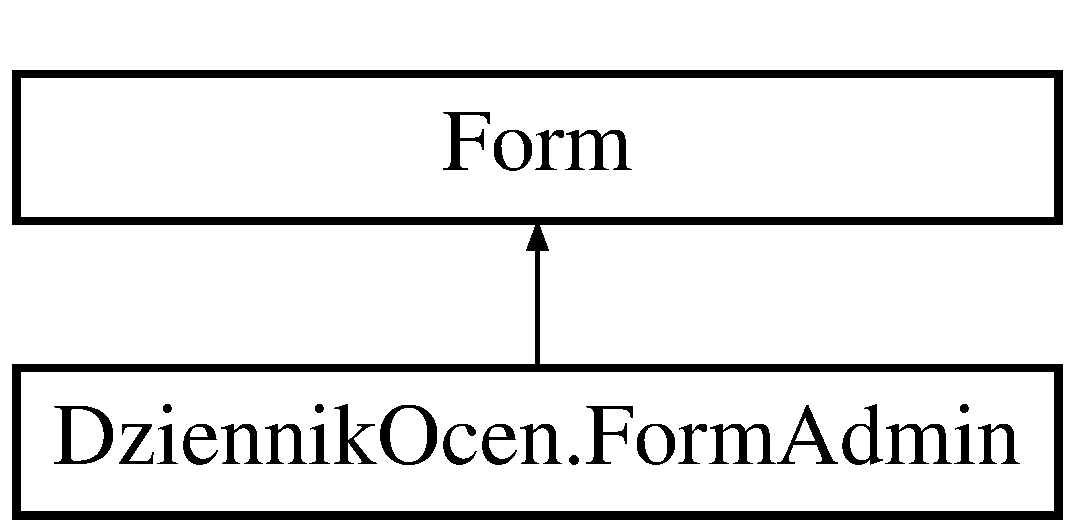
\includegraphics[height=2.000000cm]{class_dziennik_ocen_1_1_form_admin}
\end{center}
\end{figure}
\subsection*{Public Member Functions}
\begin{DoxyCompactItemize}
\item 
\hyperlink{class_dziennik_ocen_1_1_form_admin_a56c723984192ed6599a2f426a7b03b56}{Form\+Admin} ()
\end{DoxyCompactItemize}
\subsection*{Protected Member Functions}
\begin{DoxyCompactItemize}
\item 
override void \hyperlink{class_dziennik_ocen_1_1_form_admin_a226138ac8da3cb8b2064e61823c13a3a}{Dispose} (bool disposing)
\begin{DoxyCompactList}\small\item\em Clean up any resources being used. \end{DoxyCompactList}\end{DoxyCompactItemize}
\subsection*{Private Member Functions}
\begin{DoxyCompactItemize}
\item 
void \hyperlink{class_dziennik_ocen_1_1_form_admin_a6f9e595eba987ac552ed9a539e046e0e}{Form\+Admin\+\_\+\+Resize} (object sender, Event\+Args e)
\item 
void \hyperlink{class_dziennik_ocen_1_1_form_admin_a30578c22b6800b08b088a6bce866cc89}{Get\+Data\+Grupa} (string select\+Command, Data\+Grid\+View dgv, Binding\+Source bs)
\item 
void \hyperlink{class_dziennik_ocen_1_1_form_admin_a1d5c0be82fed48ef5de771ecce613e0b}{Get\+Data\+Przedmiot} (string select\+Command, Data\+Grid\+View dgv, Binding\+Source bs)
\item 
void \hyperlink{class_dziennik_ocen_1_1_form_admin_a78cfb7e0267d3e80e20843d72ef29a16}{Get\+Data\+Projekt} (string select\+Command, Data\+Grid\+View dgv, Binding\+Source bs)
\item 
void \hyperlink{class_dziennik_ocen_1_1_form_admin_a3473aad7b3aff3e8542c2d87c73167d8}{Get\+Data\+Student} (string select\+Command, Data\+Grid\+View dgv, Binding\+Source bs)
\item 
void \hyperlink{class_dziennik_ocen_1_1_form_admin_af98b8f3bf331570a6d1215b13cf054ef}{Get\+Data\+Prowadzacy} (string select\+Command, Data\+Grid\+View dgv, Binding\+Source bs)
\item 
void \hyperlink{class_dziennik_ocen_1_1_form_admin_a43df04f474ae6762b971c1d1e57d0db3}{Get\+Data\+Projekty} (string select\+Command, Data\+Grid\+View dgv, Binding\+Source bs)
\item 
void \hyperlink{class_dziennik_ocen_1_1_form_admin_a60dde3b0c4b2b71927a15b9240f2a760}{Get\+Data\+Przedmioty} (string select\+Command, Data\+Grid\+View dgv, Binding\+Source bs)
\item 
void \hyperlink{class_dziennik_ocen_1_1_form_admin_a164792e99a2213c5e62870c2ffee0d31}{dgv\+Student\+\_\+\+Cell\+End\+Edit} (object sender, Data\+Grid\+View\+Cell\+Event\+Args e)
\item 
void \hyperlink{class_dziennik_ocen_1_1_form_admin_a3b95eb1c804963f3ea3b3650c71ea4f0}{dgv\+Grupa\+\_\+\+Cell\+End\+Edit} (object sender, Data\+Grid\+View\+Cell\+Event\+Args e)
\item 
void \hyperlink{class_dziennik_ocen_1_1_form_admin_adf080cf9bf6ce910be2b1b539c5c6bc2}{dgv\+Przedmiot\+\_\+\+Cell\+End\+Edit} (object sender, Data\+Grid\+View\+Cell\+Event\+Args e)
\item 
void \hyperlink{class_dziennik_ocen_1_1_form_admin_a2f6a990aa7890c543a9b7d6cda212884}{dgv\+Projekt\+\_\+\+Cell\+End\+Edit} (object sender, Data\+Grid\+View\+Cell\+Event\+Args e)
\item 
void \hyperlink{class_dziennik_ocen_1_1_form_admin_a0b39905ac3fcb424c1d12975643712fa}{dgv\+Prowadzacy\+\_\+\+Cell\+End\+Edit} (object sender, Data\+Grid\+View\+Cell\+Event\+Args e)
\item 
void \hyperlink{class_dziennik_ocen_1_1_form_admin_a8041f9fec5afec151944bd5eeb7897c8}{dgv\+Projekty\+\_\+\+Cell\+End\+Edit} (object sender, Data\+Grid\+View\+Cell\+Event\+Args e)
\item 
void \hyperlink{class_dziennik_ocen_1_1_form_admin_ace196eca0cd55af280cb7e4a1a75a540}{dgv\+Przedmioty\+\_\+\+Cell\+End\+Edit} (object sender, Data\+Grid\+View\+Cell\+Event\+Args e)
\item 
void \hyperlink{class_dziennik_ocen_1_1_form_admin_a7633d40ff0076c9b931e533e24657801}{btn\+Dodaj\+Student\+\_\+\+Click} (object sender, Event\+Args e)
\item 
void \hyperlink{class_dziennik_ocen_1_1_form_admin_ac3dfb3b4fe0ed9e8a8f4dd8398e49823}{btn\+Dodaj\+Grupa\+\_\+\+Click} (object sender, Event\+Args e)
\item 
void \hyperlink{class_dziennik_ocen_1_1_form_admin_ad6d63eaff7b29753a359f638c130d54b}{btn\+Dodaj\+Przedmiot\+\_\+\+Click} (object sender, Event\+Args e)
\item 
void \hyperlink{class_dziennik_ocen_1_1_form_admin_a858b46657974fd92e0e4208dba8f4048}{btn\+Dodaj\+Projekt\+\_\+\+Click} (object sender, Event\+Args e)
\item 
void \hyperlink{class_dziennik_ocen_1_1_form_admin_a51a25d236307419c723310933f6a5440}{btn\+Dodaj\+Prowadzacy\+\_\+\+Click} (object sender, Event\+Args e)
\item 
void \hyperlink{class_dziennik_ocen_1_1_form_admin_a4f8a7e8bcbc364b7f2ca67d9bc306ab3}{btn\+Dodaj\+Projekty\+\_\+\+Click} (object sender, Event\+Args e)
\item 
void \hyperlink{class_dziennik_ocen_1_1_form_admin_a8931bc3365519fec70d38e714151f1ce}{btn\+Dodaj\+Przedmioty\+\_\+\+Click} (object sender, Event\+Args e)
\item 
void \hyperlink{class_dziennik_ocen_1_1_form_admin_a349ce3b1eeed9027c70615a77d250a5d}{dgv\+Grupa\+\_\+\+User\+Deleting\+Row} (object sender, Data\+Grid\+View\+Row\+Cancel\+Event\+Args e)
\item 
void \hyperlink{class_dziennik_ocen_1_1_form_admin_a5ff03e7113d930afdf9d0c651734fae0}{dgv\+Przedmiot\+\_\+\+User\+Deleting\+Row} (object sender, Data\+Grid\+View\+Row\+Cancel\+Event\+Args e)
\item 
void \hyperlink{class_dziennik_ocen_1_1_form_admin_ad25ef9fe40bb0f7d995b07c10e053c3d}{dgv\+Projekt\+\_\+\+User\+Deleting\+Row} (object sender, Data\+Grid\+View\+Row\+Cancel\+Event\+Args e)
\item 
void \hyperlink{class_dziennik_ocen_1_1_form_admin_af3ef7cac8cbb4acf92efdd1c3d278647}{dgv\+Student\+\_\+\+User\+Deleting\+Row} (object sender, Data\+Grid\+View\+Row\+Cancel\+Event\+Args e)
\item 
void \hyperlink{class_dziennik_ocen_1_1_form_admin_aaf3a81a886da60aae87a34b5ca2e3d4d}{dgv\+Prowadzacy\+\_\+\+User\+Deleting\+Row} (object sender, Data\+Grid\+View\+Row\+Cancel\+Event\+Args e)
\item 
void \hyperlink{class_dziennik_ocen_1_1_form_admin_a48466d6cfac9af36f0a581af601f7906}{dgv\+Projekty\+\_\+\+User\+Deleting\+Row} (object sender, Data\+Grid\+View\+Row\+Cancel\+Event\+Args e)
\item 
void \hyperlink{class_dziennik_ocen_1_1_form_admin_a3e68e6b9a8298d9e207cb0aba20b161b}{dgv\+Przedmioty\+\_\+\+User\+Deleting\+Row} (object sender, Data\+Grid\+View\+Row\+Cancel\+Event\+Args e)
\item 
void \hyperlink{class_dziennik_ocen_1_1_form_admin_a751a9f0c3a418edabd1f6ce4d78d4ceb}{Form\+Admin\+\_\+\+Form\+Closing} (object sender, Form\+Closing\+Event\+Args e)
\item 
void \hyperlink{class_dziennik_ocen_1_1_form_admin_a876a136e8c48ca102cc44b34c5993c43}{Initialize\+Component} ()
\begin{DoxyCompactList}\small\item\em Required method for Designer support -\/ do not modify the contents of this method with the code editor. \end{DoxyCompactList}\end{DoxyCompactItemize}
\subsection*{Private Attributes}
\begin{DoxyCompactItemize}
\item 
\hyperlink{class_dziennik_ocen_1_1_dziennik_ocen_entities}{Dziennik\+Ocen\+Entities} \hyperlink{class_dziennik_ocen_1_1_form_admin_a77a65310263c63d03f167e6099dc4bc8}{db} = new \hyperlink{class_dziennik_ocen_1_1_dziennik_ocen_entities}{Dziennik\+Ocen\+Entities}()
\item 
int \hyperlink{class_dziennik_ocen_1_1_form_admin_a2802bf47fadb6ecc1ccf40a94e065d05}{form\+Height}
\item 
int \hyperlink{class_dziennik_ocen_1_1_form_admin_a2abc13ba3dc7102aa96ce608fcb1fd9c}{form\+Width}
\item 
int \hyperlink{class_dziennik_ocen_1_1_form_admin_a3ddc4920ca4ca7352739035f2afd5341}{zapis}
\item 
Sql\+Data\+Adapter \hyperlink{class_dziennik_ocen_1_1_form_admin_af4bcf765df04fbfac6cc99f1e911210b}{da\+Grupa} = new Sql\+Data\+Adapter()
\item 
Sql\+Data\+Adapter \hyperlink{class_dziennik_ocen_1_1_form_admin_a32d386bedadefccecfb5a7667f5aefb7}{da\+Przedmiot} = new Sql\+Data\+Adapter()
\item 
Sql\+Data\+Adapter \hyperlink{class_dziennik_ocen_1_1_form_admin_aa855b7aa18748501f995cd4bd664e8a5}{da\+Projekt} = new Sql\+Data\+Adapter()
\item 
Sql\+Data\+Adapter \hyperlink{class_dziennik_ocen_1_1_form_admin_a72ffbfd2d1b16625886143ba255e08e9}{da\+Student} = new Sql\+Data\+Adapter()
\item 
Sql\+Data\+Adapter \hyperlink{class_dziennik_ocen_1_1_form_admin_a182d378addcef222536f9c514f85a703}{da\+Prowadzacy} = new Sql\+Data\+Adapter()
\item 
Sql\+Data\+Adapter \hyperlink{class_dziennik_ocen_1_1_form_admin_ab7869a1097cd333154336f7f3008295c}{da\+Projekty} = new Sql\+Data\+Adapter()
\item 
Sql\+Data\+Adapter \hyperlink{class_dziennik_ocen_1_1_form_admin_a906f1b10c5e6a0a937e7cd281952cf9e}{da\+Przedmioty} = new Sql\+Data\+Adapter()
\item 
Sql\+Command\+Builder \hyperlink{class_dziennik_ocen_1_1_form_admin_ad78cf92a31e4ac705fc1b07f91eccf12}{command\+Builder}
\item 
Data\+Set \hyperlink{class_dziennik_ocen_1_1_form_admin_aead339c7648bc14d61f61eb9192157e2}{dataset} = new Data\+Set()
\item 
System.\+Component\+Model.\+I\+Container \hyperlink{class_dziennik_ocen_1_1_form_admin_add4f712ca83ab265bf5dc023ae8b7a49}{components} = null
\begin{DoxyCompactList}\small\item\em Required designer variable. \end{DoxyCompactList}\item 
System.\+Windows.\+Forms.\+Data\+Grid\+View \hyperlink{class_dziennik_ocen_1_1_form_admin_a2e704158d9e4b76e3d75c77c6a41c577}{dgv\+Grupa}
\item 
System.\+Windows.\+Forms.\+Data\+Grid\+View \hyperlink{class_dziennik_ocen_1_1_form_admin_a9120bd1ad60f426475791e60ccdd0204}{dgv\+Przedmiot}
\item 
System.\+Windows.\+Forms.\+Data\+Grid\+View \hyperlink{class_dziennik_ocen_1_1_form_admin_a0f7bd114b47cd8b11a067b5f0dbe9f3f}{dgv\+Student}
\item 
System.\+Windows.\+Forms.\+Data\+Grid\+View \hyperlink{class_dziennik_ocen_1_1_form_admin_a10132ded0fc33de4056568a632e598c7}{dgv\+Prowadzacy}
\item 
System.\+Windows.\+Forms.\+Data\+Grid\+View \hyperlink{class_dziennik_ocen_1_1_form_admin_a54f958ca831b5544020cfdfc7e0ece9a}{dgv\+Projekty}
\item 
System.\+Windows.\+Forms.\+Data\+Grid\+View \hyperlink{class_dziennik_ocen_1_1_form_admin_aecd123ff4d179ae6392fed78530377f0}{dgv\+Przedmioty}
\item 
System.\+Windows.\+Forms.\+Data\+Grid\+View \hyperlink{class_dziennik_ocen_1_1_form_admin_ade721ef47de208cef1144d075432f31f}{dgv\+Projekt}
\item 
System.\+Windows.\+Forms.\+Binding\+Source \hyperlink{class_dziennik_ocen_1_1_form_admin_a05c33963ce3177b48999725fc766ed75}{bs\+Grupa}
\item 
System.\+Windows.\+Forms.\+Binding\+Source \hyperlink{class_dziennik_ocen_1_1_form_admin_ab0adea8acde680ff8e2ad0329b526a97}{bs\+Przedmiot}
\item 
System.\+Windows.\+Forms.\+Binding\+Source \hyperlink{class_dziennik_ocen_1_1_form_admin_a1c7f6c81ca582f263c66fc2be3928661}{bs\+Student}
\item 
System.\+Windows.\+Forms.\+Binding\+Source \hyperlink{class_dziennik_ocen_1_1_form_admin_a32118b2507f71e59c520449711857dba}{bs\+Prowadzacy}
\item 
System.\+Windows.\+Forms.\+Binding\+Source \hyperlink{class_dziennik_ocen_1_1_form_admin_af48204622d8aca29dceb4935b9e272c1}{bs\+Projekty}
\item 
System.\+Windows.\+Forms.\+Binding\+Source \hyperlink{class_dziennik_ocen_1_1_form_admin_a5de64a16e387981ee49506b801945ddd}{bs\+Przedmioty}
\item 
System.\+Windows.\+Forms.\+Binding\+Source \hyperlink{class_dziennik_ocen_1_1_form_admin_a262a31373e35cec908134bb01d7bd135}{bs\+Projekt}
\item 
System.\+Windows.\+Forms.\+Button \hyperlink{class_dziennik_ocen_1_1_form_admin_a2c9c13e11214db9b7bd7d38e5b0d702c}{btn\+Dodaj\+Student}
\item 
System.\+Windows.\+Forms.\+Button \hyperlink{class_dziennik_ocen_1_1_form_admin_ab81e4a1037f33b0ac3125dcf9b589719}{btn\+Dodaj\+Grupa}
\item 
System.\+Windows.\+Forms.\+Button \hyperlink{class_dziennik_ocen_1_1_form_admin_a9e9f56e615db94726ec5f84c955c0a77}{btn\+Dodaj\+Projekt}
\item 
System.\+Windows.\+Forms.\+Button \hyperlink{class_dziennik_ocen_1_1_form_admin_a9d0807ac61806a6c11d6d8d803fae334}{btn\+Dodaj\+Przedmiot}
\item 
System.\+Windows.\+Forms.\+Button \hyperlink{class_dziennik_ocen_1_1_form_admin_a78c6935670aa636d9fa2db119065a924}{btn\+Dodaj\+Prowadzacy}
\item 
System.\+Windows.\+Forms.\+Button \hyperlink{class_dziennik_ocen_1_1_form_admin_ad5380dd7001fab173e85b01893731451}{btn\+Dodaj\+Przedmioty}
\item 
System.\+Windows.\+Forms.\+Button \hyperlink{class_dziennik_ocen_1_1_form_admin_a04cc551c6f19adc7cc95f84ce7b3c390}{btn\+Dodaj\+Projekty}
\item 
System.\+Windows.\+Forms.\+Data\+Grid\+View\+Text\+Box\+Column \hyperlink{class_dziennik_ocen_1_1_form_admin_a9a5627214167e623fdaf816913955845}{email\+Data\+Grid\+View\+Text\+Box\+Column1}
\item 
System.\+Windows.\+Forms.\+Data\+Grid\+View\+Text\+Box\+Column \hyperlink{class_dziennik_ocen_1_1_form_admin_a282e652aef3c33335c0ad609a65b0006}{ocenaprzedmiotu\+Data\+Grid\+View\+Text\+Box\+Column}
\item 
System.\+Windows.\+Forms.\+Data\+Grid\+View\+Text\+Box\+Column \hyperlink{class_dziennik_ocen_1_1_form_admin_a95f6cc81f2184385fc78c287488d630d}{id\+G\+R\+U\+P\+Y\+Data\+Grid\+View\+Text\+Box\+Column}
\item 
System.\+Windows.\+Forms.\+Data\+Grid\+View\+Text\+Box\+Column \hyperlink{class_dziennik_ocen_1_1_form_admin_abc8ecccfd2a3b07c6a5e51a89f4916c4}{nazwagrupy\+Data\+Grid\+View\+Text\+Box\+Column}
\item 
System.\+Windows.\+Forms.\+Data\+Grid\+View\+Text\+Box\+Column \hyperlink{class_dziennik_ocen_1_1_form_admin_a6917f007b27f260cce5ecfd24aa351f7}{S\+T\+U\+D\+E\+N\+T\+Data\+Grid\+View\+Text\+Box\+Column}
\item 
System.\+Windows.\+Forms.\+Data\+Grid\+View\+Text\+Box\+Column \hyperlink{class_dziennik_ocen_1_1_form_admin_a26e4a3fa2dc997dc2639bad664efcf95}{id\+P\+R\+Z\+E\+D\+M\+I\+O\+T\+U\+Data\+Grid\+View\+Text\+Box\+Column}
\item 
System.\+Windows.\+Forms.\+Data\+Grid\+View\+Text\+Box\+Column \hyperlink{class_dziennik_ocen_1_1_form_admin_aabccbc0a74ca00a35018db908f23d017}{nazwaprzedmiotu\+Data\+Grid\+View\+Text\+Box\+Column}
\item 
System.\+Windows.\+Forms.\+Data\+Grid\+View\+Text\+Box\+Column \hyperlink{class_dziennik_ocen_1_1_form_admin_afa13eec734673382f86da87f33c5e52c}{opisprzedmiotu\+Data\+Grid\+View\+Text\+Box\+Column}
\item 
System.\+Windows.\+Forms.\+Data\+Grid\+View\+Text\+Box\+Column \hyperlink{class_dziennik_ocen_1_1_form_admin_a0680998f0013ced8888ab26f994b4312}{e\+C\+T\+S\+Data\+Grid\+View\+Text\+Box\+Column}
\item 
System.\+Windows.\+Forms.\+Data\+Grid\+View\+Text\+Box\+Column \hyperlink{class_dziennik_ocen_1_1_form_admin_a725b610994a951c46baa95371ca45e19}{p\+R\+O\+J\+E\+K\+T\+Data\+Grid\+View\+Text\+Box\+Column}
\item 
System.\+Windows.\+Forms.\+Data\+Grid\+View\+Text\+Box\+Column \hyperlink{class_dziennik_ocen_1_1_form_admin_aeab4a6aad13107f7f5e9fc5d6a61f803}{przedmioty\+Data\+Grid\+View\+Text\+Box\+Column}
\item 
System.\+Windows.\+Forms.\+Data\+Grid\+View\+Text\+Box\+Column \hyperlink{class_dziennik_ocen_1_1_form_admin_a9e981188d1513025f31ea53b1e54fe86}{id\+S\+T\+U\+D\+E\+N\+T\+A\+Data\+Grid\+View\+Text\+Box\+Column}
\item 
System.\+Windows.\+Forms.\+Data\+Grid\+View\+Text\+Box\+Column \hyperlink{class_dziennik_ocen_1_1_form_admin_aad503d02e5dd2a769147167a75af6af6}{id\+G\+R\+U\+P\+Y\+Data\+Grid\+View\+Text\+Box\+Column1}
\item 
System.\+Windows.\+Forms.\+Data\+Grid\+View\+Text\+Box\+Column \hyperlink{class_dziennik_ocen_1_1_form_admin_ad2c069cbc1f999203c0c1321be68d3df}{imie\+Data\+Grid\+View\+Text\+Box\+Column}
\item 
System.\+Windows.\+Forms.\+Data\+Grid\+View\+Text\+Box\+Column \hyperlink{class_dziennik_ocen_1_1_form_admin_aab4cfa6124fdde86f95e8c79c5c23406}{nazwisko\+Data\+Grid\+View\+Text\+Box\+Column}
\item 
System.\+Windows.\+Forms.\+Data\+Grid\+View\+Text\+Box\+Column \hyperlink{class_dziennik_ocen_1_1_form_admin_a72a251b150573a626647791876332015}{telefon\+Data\+Grid\+View\+Text\+Box\+Column}
\item 
System.\+Windows.\+Forms.\+Data\+Grid\+View\+Text\+Box\+Column \hyperlink{class_dziennik_ocen_1_1_form_admin_a06a64f75c8ce9a7c86ffdc6120741268}{adres\+Data\+Grid\+View\+Text\+Box\+Column}
\item 
System.\+Windows.\+Forms.\+Data\+Grid\+View\+Text\+Box\+Column \hyperlink{class_dziennik_ocen_1_1_form_admin_aaa3365a57ff352db1b165745e6631cb1}{e\+\_\+mail}
\item 
System.\+Windows.\+Forms.\+Data\+Grid\+View\+Text\+Box\+Column \hyperlink{class_dziennik_ocen_1_1_form_admin_a013f9ee1a23f86778e6c66155b1bf93e}{haslo\+Data\+Grid\+View\+Text\+Box\+Column}
\item 
System.\+Windows.\+Forms.\+Data\+Grid\+View\+Text\+Box\+Column \hyperlink{class_dziennik_ocen_1_1_form_admin_a6fc44af8dd2ad779199a11f1a2a3769d}{g\+R\+U\+P\+A\+Data\+Grid\+View\+Text\+Box\+Column}
\item 
System.\+Windows.\+Forms.\+Data\+Grid\+View\+Text\+Box\+Column \hyperlink{class_dziennik_ocen_1_1_form_admin_ac4aa25c3b282b8c8380d768559c95423}{projekty\+Data\+Grid\+View\+Text\+Box\+Column1}
\item 
System.\+Windows.\+Forms.\+Data\+Grid\+View\+Text\+Box\+Column \hyperlink{class_dziennik_ocen_1_1_form_admin_a227b182179159f912355b73406334336}{przedmioty\+Data\+Grid\+View\+Text\+Box\+Column1}
\item 
System.\+Windows.\+Forms.\+Data\+Grid\+View\+Text\+Box\+Column \hyperlink{class_dziennik_ocen_1_1_form_admin_a16d7e9e45a12e277f55ccfefedc4828e}{id\+P\+R\+O\+W\+A\+D\+ZĄ\+C\+E\+G\+O\+Data\+Grid\+View\+Text\+Box\+Column}
\item 
System.\+Windows.\+Forms.\+Data\+Grid\+View\+Text\+Box\+Column \hyperlink{class_dziennik_ocen_1_1_form_admin_a683c4a5df19d58a88cb375268f1f1216}{imie\+Data\+Grid\+View\+Text\+Box\+Column1}
\item 
System.\+Windows.\+Forms.\+Data\+Grid\+View\+Text\+Box\+Column \hyperlink{class_dziennik_ocen_1_1_form_admin_aa39a72b1739cdea4f0b46b03fcb35cd1}{nazwisko\+Data\+Grid\+View\+Text\+Box\+Column1}
\item 
System.\+Windows.\+Forms.\+Data\+Grid\+View\+Text\+Box\+Column \hyperlink{class_dziennik_ocen_1_1_form_admin_ade0d90058a355376268b3b0a4ae1444d}{telefon\+Data\+Grid\+View\+Text\+Box\+Column1}
\item 
System.\+Windows.\+Forms.\+Data\+Grid\+View\+Text\+Box\+Column \hyperlink{class_dziennik_ocen_1_1_form_admin_a1ab2395ad14f3e0ff677a5d1bc44a6cc}{adres\+Data\+Grid\+View\+Text\+Box\+Column1}
\item 
System.\+Windows.\+Forms.\+Data\+Grid\+View\+Text\+Box\+Column \hyperlink{class_dziennik_ocen_1_1_form_admin_a7b9bbbd7c6bb6feef518a46ac79e5da5}{data\+Grid\+View\+Text\+Box\+Column1}
\item 
System.\+Windows.\+Forms.\+Data\+Grid\+View\+Text\+Box\+Column \hyperlink{class_dziennik_ocen_1_1_form_admin_a8864db3ba24c0e8c5b6d6aa3a1278601}{haslo\+Data\+Grid\+View\+Text\+Box\+Column1}
\item 
System.\+Windows.\+Forms.\+Data\+Grid\+View\+Text\+Box\+Column \hyperlink{class_dziennik_ocen_1_1_form_admin_a2b1066cdc430cd7724666a0a95101a3c}{stanowisko\+Data\+Grid\+View\+Text\+Box\+Column}
\item 
System.\+Windows.\+Forms.\+Data\+Grid\+View\+Text\+Box\+Column \hyperlink{class_dziennik_ocen_1_1_form_admin_ad8c0bca7b6b119720ec43f183c252098}{projekty\+Data\+Grid\+View\+Text\+Box\+Column2}
\item 
System.\+Windows.\+Forms.\+Data\+Grid\+View\+Text\+Box\+Column \hyperlink{class_dziennik_ocen_1_1_form_admin_a764a027534438bf1f2f777a31e904eb6}{przedmioty\+Data\+Grid\+View\+Text\+Box\+Column2}
\item 
System.\+Windows.\+Forms.\+Data\+Grid\+View\+Text\+Box\+Column \hyperlink{class_dziennik_ocen_1_1_form_admin_a43f85f7570d8f173c58c95cd8096ec83}{id\+S\+T\+U\+D\+E\+N\+T\+A\+Data\+Grid\+View\+Text\+Box\+Column1}
\item 
System.\+Windows.\+Forms.\+Data\+Grid\+View\+Text\+Box\+Column \hyperlink{class_dziennik_ocen_1_1_form_admin_aa0b03d605064fd0226fbd650ab4d2194}{id\+P\+R\+O\+J\+E\+K\+T\+U\+Data\+Grid\+View\+Text\+Box\+Column1}
\item 
System.\+Windows.\+Forms.\+Data\+Grid\+View\+Text\+Box\+Column \hyperlink{class_dziennik_ocen_1_1_form_admin_abade19cddc1e6c43a13de0d126e3ca62}{id\+P\+R\+O\+W\+A\+D\+ZĄ\+C\+E\+G\+O\+Data\+Grid\+View\+Text\+Box\+Column1}
\item 
System.\+Windows.\+Forms.\+Data\+Grid\+View\+Text\+Box\+Column \hyperlink{class_dziennik_ocen_1_1_form_admin_a3fb6f3b8f64792f8555efcfb1046d437}{ocenaprojektu\+Data\+Grid\+View\+Text\+Box\+Column}
\item 
System.\+Windows.\+Forms.\+Data\+Grid\+View\+Text\+Box\+Column \hyperlink{class_dziennik_ocen_1_1_form_admin_a43c82d7a21405323bffbfb18b098d8be}{dataprojektu\+Data\+Grid\+View\+Text\+Box\+Column}
\item 
System.\+Windows.\+Forms.\+Data\+Grid\+View\+Text\+Box\+Column \hyperlink{class_dziennik_ocen_1_1_form_admin_aa341fdd2dc8d4bbd2cd2c7507659d1be}{uwagiprojektu\+Data\+Grid\+View\+Text\+Box\+Column}
\item 
System.\+Windows.\+Forms.\+Data\+Grid\+View\+Text\+Box\+Column \hyperlink{class_dziennik_ocen_1_1_form_admin_a087289edfa65048d97c755990d69d888}{p\+R\+O\+J\+E\+K\+T\+Data\+Grid\+View\+Text\+Box\+Column1}
\item 
System.\+Windows.\+Forms.\+Data\+Grid\+View\+Text\+Box\+Column \hyperlink{class_dziennik_ocen_1_1_form_admin_ae8a41e16c66289a859a7e055a4bfdaff}{p\+R\+O\+W\+A\+D\+ZĄ\+C\+Y\+Data\+Grid\+View\+Text\+Box\+Column}
\item 
System.\+Windows.\+Forms.\+Data\+Grid\+View\+Text\+Box\+Column \hyperlink{class_dziennik_ocen_1_1_form_admin_aa3f656e0a43ec42e4360d5bb67ffe0e0}{s\+T\+U\+D\+E\+N\+T\+Data\+Grid\+View\+Text\+Box\+Column1}
\item 
System.\+Windows.\+Forms.\+Data\+Grid\+View\+Text\+Box\+Column \hyperlink{class_dziennik_ocen_1_1_form_admin_a99a7ea058c945554d9165056687bc3a7}{id\+P\+R\+O\+J\+E\+K\+T\+U\+Data\+Grid\+View\+Text\+Box\+Column}
\item 
System.\+Windows.\+Forms.\+Data\+Grid\+View\+Text\+Box\+Column \hyperlink{class_dziennik_ocen_1_1_form_admin_ad35482b5eb4ba1ea7241a6cb83155e9c}{id\+P\+R\+Z\+E\+D\+M\+I\+O\+T\+U\+Data\+Grid\+View\+Text\+Box\+Column1}
\item 
System.\+Windows.\+Forms.\+Data\+Grid\+View\+Text\+Box\+Column \hyperlink{class_dziennik_ocen_1_1_form_admin_a9917716fd8b31205ca04f892f6973a3e}{nazwaprojektu\+Data\+Grid\+View\+Text\+Box\+Column}
\item 
System.\+Windows.\+Forms.\+Data\+Grid\+View\+Text\+Box\+Column \hyperlink{class_dziennik_ocen_1_1_form_admin_a4e784a85cb96c95d2295d6106268792f}{opisprojektu\+Data\+Grid\+View\+Text\+Box\+Column}
\item 
System.\+Windows.\+Forms.\+Data\+Grid\+View\+Text\+Box\+Column \hyperlink{class_dziennik_ocen_1_1_form_admin_a8888f586a33e8fa383b5fd20947acf53}{p\+R\+Z\+E\+D\+M\+I\+O\+T\+Data\+Grid\+View\+Text\+Box\+Column}
\item 
System.\+Windows.\+Forms.\+Data\+Grid\+View\+Text\+Box\+Column \hyperlink{class_dziennik_ocen_1_1_form_admin_acd8b38a410aab8b25bb1e5fa9077b056}{projekty\+Data\+Grid\+View\+Text\+Box\+Column}
\item 
System.\+Windows.\+Forms.\+Data\+Grid\+View\+Text\+Box\+Column \hyperlink{class_dziennik_ocen_1_1_form_admin_add0f83e810a64b6633a7681fb590a232}{id\+S\+T\+U\+D\+E\+N\+T\+A\+Data\+Grid\+View\+Text\+Box\+Column2}
\item 
System.\+Windows.\+Forms.\+Data\+Grid\+View\+Text\+Box\+Column \hyperlink{class_dziennik_ocen_1_1_form_admin_a11d4f04b47905b536faf7ad754965fec}{id\+P\+R\+O\+W\+A\+D\+ZĄ\+C\+E\+G\+O\+Data\+Grid\+View\+Text\+Box\+Column2}
\item 
System.\+Windows.\+Forms.\+Data\+Grid\+View\+Text\+Box\+Column \hyperlink{class_dziennik_ocen_1_1_form_admin_a2e1c5c7ed8ee06604fff20abcadbe193}{id\+P\+R\+Z\+E\+D\+M\+I\+O\+T\+U\+Data\+Grid\+View\+Text\+Box\+Column2}
\item 
System.\+Windows.\+Forms.\+Data\+Grid\+View\+Text\+Box\+Column \hyperlink{class_dziennik_ocen_1_1_form_admin_ad0e7bec9f88f5562daa2ef39251ae18f}{ocena\+\_\+przedmiotu}
\item 
System.\+Windows.\+Forms.\+Data\+Grid\+View\+Text\+Box\+Column \hyperlink{class_dziennik_ocen_1_1_form_admin_a1e12e925c65d4f38e5a3cb3a490c47e6}{datazaliczeniaprzedmiotu\+Data\+Grid\+View\+Text\+Box\+Column}
\item 
System.\+Windows.\+Forms.\+Data\+Grid\+View\+Text\+Box\+Column \hyperlink{class_dziennik_ocen_1_1_form_admin_a79c1dedbf916f5d973bb341600309f8d}{uwagiprzedmiotu\+Data\+Grid\+View\+Text\+Box\+Column}
\item 
System.\+Windows.\+Forms.\+Data\+Grid\+View\+Text\+Box\+Column \hyperlink{class_dziennik_ocen_1_1_form_admin_a53b38f04a035a58f34d8ce1f63ee60f1}{p\+R\+O\+W\+A\+D\+ZĄ\+C\+Y\+Data\+Grid\+View\+Text\+Box\+Column1}
\item 
System.\+Windows.\+Forms.\+Data\+Grid\+View\+Text\+Box\+Column \hyperlink{class_dziennik_ocen_1_1_form_admin_af140ea06c84a962f3b880ce5e4b043d3}{s\+T\+U\+D\+E\+N\+T\+Data\+Grid\+View\+Text\+Box\+Column2}
\item 
System.\+Windows.\+Forms.\+Data\+Grid\+View\+Text\+Box\+Column \hyperlink{class_dziennik_ocen_1_1_form_admin_a07c80c90ba741ffe4ad7583fede66f15}{p\+R\+Z\+E\+D\+M\+I\+O\+T\+Data\+Grid\+View\+Text\+Box\+Column1}
\end{DoxyCompactItemize}


\subsection{Constructor \& Destructor Documentation}
\mbox{\Hypertarget{class_dziennik_ocen_1_1_form_admin_a56c723984192ed6599a2f426a7b03b56}\label{class_dziennik_ocen_1_1_form_admin_a56c723984192ed6599a2f426a7b03b56}} 
\index{Dziennik\+Ocen\+::\+Form\+Admin@{Dziennik\+Ocen\+::\+Form\+Admin}!Form\+Admin@{Form\+Admin}}
\index{Form\+Admin@{Form\+Admin}!Dziennik\+Ocen\+::\+Form\+Admin@{Dziennik\+Ocen\+::\+Form\+Admin}}
\subsubsection{\texorpdfstring{Form\+Admin()}{FormAdmin()}}
{\footnotesize\ttfamily Dziennik\+Ocen.\+Form\+Admin.\+Form\+Admin (\begin{DoxyParamCaption}{ }\end{DoxyParamCaption})\hspace{0.3cm}{\ttfamily [inline]}}



\subsection{Member Function Documentation}
\mbox{\Hypertarget{class_dziennik_ocen_1_1_form_admin_ac3dfb3b4fe0ed9e8a8f4dd8398e49823}\label{class_dziennik_ocen_1_1_form_admin_ac3dfb3b4fe0ed9e8a8f4dd8398e49823}} 
\index{Dziennik\+Ocen\+::\+Form\+Admin@{Dziennik\+Ocen\+::\+Form\+Admin}!btn\+Dodaj\+Grupa\+\_\+\+Click@{btn\+Dodaj\+Grupa\+\_\+\+Click}}
\index{btn\+Dodaj\+Grupa\+\_\+\+Click@{btn\+Dodaj\+Grupa\+\_\+\+Click}!Dziennik\+Ocen\+::\+Form\+Admin@{Dziennik\+Ocen\+::\+Form\+Admin}}
\subsubsection{\texorpdfstring{btn\+Dodaj\+Grupa\+\_\+\+Click()}{btnDodajGrupa\_Click()}}
{\footnotesize\ttfamily void Dziennik\+Ocen.\+Form\+Admin.\+btn\+Dodaj\+Grupa\+\_\+\+Click (\begin{DoxyParamCaption}\item[{object}]{sender,  }\item[{Event\+Args}]{e }\end{DoxyParamCaption})\hspace{0.3cm}{\ttfamily [inline]}, {\ttfamily [private]}}

\mbox{\Hypertarget{class_dziennik_ocen_1_1_form_admin_a858b46657974fd92e0e4208dba8f4048}\label{class_dziennik_ocen_1_1_form_admin_a858b46657974fd92e0e4208dba8f4048}} 
\index{Dziennik\+Ocen\+::\+Form\+Admin@{Dziennik\+Ocen\+::\+Form\+Admin}!btn\+Dodaj\+Projekt\+\_\+\+Click@{btn\+Dodaj\+Projekt\+\_\+\+Click}}
\index{btn\+Dodaj\+Projekt\+\_\+\+Click@{btn\+Dodaj\+Projekt\+\_\+\+Click}!Dziennik\+Ocen\+::\+Form\+Admin@{Dziennik\+Ocen\+::\+Form\+Admin}}
\subsubsection{\texorpdfstring{btn\+Dodaj\+Projekt\+\_\+\+Click()}{btnDodajProjekt\_Click()}}
{\footnotesize\ttfamily void Dziennik\+Ocen.\+Form\+Admin.\+btn\+Dodaj\+Projekt\+\_\+\+Click (\begin{DoxyParamCaption}\item[{object}]{sender,  }\item[{Event\+Args}]{e }\end{DoxyParamCaption})\hspace{0.3cm}{\ttfamily [inline]}, {\ttfamily [private]}}

\mbox{\Hypertarget{class_dziennik_ocen_1_1_form_admin_a4f8a7e8bcbc364b7f2ca67d9bc306ab3}\label{class_dziennik_ocen_1_1_form_admin_a4f8a7e8bcbc364b7f2ca67d9bc306ab3}} 
\index{Dziennik\+Ocen\+::\+Form\+Admin@{Dziennik\+Ocen\+::\+Form\+Admin}!btn\+Dodaj\+Projekty\+\_\+\+Click@{btn\+Dodaj\+Projekty\+\_\+\+Click}}
\index{btn\+Dodaj\+Projekty\+\_\+\+Click@{btn\+Dodaj\+Projekty\+\_\+\+Click}!Dziennik\+Ocen\+::\+Form\+Admin@{Dziennik\+Ocen\+::\+Form\+Admin}}
\subsubsection{\texorpdfstring{btn\+Dodaj\+Projekty\+\_\+\+Click()}{btnDodajProjekty\_Click()}}
{\footnotesize\ttfamily void Dziennik\+Ocen.\+Form\+Admin.\+btn\+Dodaj\+Projekty\+\_\+\+Click (\begin{DoxyParamCaption}\item[{object}]{sender,  }\item[{Event\+Args}]{e }\end{DoxyParamCaption})\hspace{0.3cm}{\ttfamily [inline]}, {\ttfamily [private]}}

\mbox{\Hypertarget{class_dziennik_ocen_1_1_form_admin_a51a25d236307419c723310933f6a5440}\label{class_dziennik_ocen_1_1_form_admin_a51a25d236307419c723310933f6a5440}} 
\index{Dziennik\+Ocen\+::\+Form\+Admin@{Dziennik\+Ocen\+::\+Form\+Admin}!btn\+Dodaj\+Prowadzacy\+\_\+\+Click@{btn\+Dodaj\+Prowadzacy\+\_\+\+Click}}
\index{btn\+Dodaj\+Prowadzacy\+\_\+\+Click@{btn\+Dodaj\+Prowadzacy\+\_\+\+Click}!Dziennik\+Ocen\+::\+Form\+Admin@{Dziennik\+Ocen\+::\+Form\+Admin}}
\subsubsection{\texorpdfstring{btn\+Dodaj\+Prowadzacy\+\_\+\+Click()}{btnDodajProwadzacy\_Click()}}
{\footnotesize\ttfamily void Dziennik\+Ocen.\+Form\+Admin.\+btn\+Dodaj\+Prowadzacy\+\_\+\+Click (\begin{DoxyParamCaption}\item[{object}]{sender,  }\item[{Event\+Args}]{e }\end{DoxyParamCaption})\hspace{0.3cm}{\ttfamily [inline]}, {\ttfamily [private]}}

\mbox{\Hypertarget{class_dziennik_ocen_1_1_form_admin_ad6d63eaff7b29753a359f638c130d54b}\label{class_dziennik_ocen_1_1_form_admin_ad6d63eaff7b29753a359f638c130d54b}} 
\index{Dziennik\+Ocen\+::\+Form\+Admin@{Dziennik\+Ocen\+::\+Form\+Admin}!btn\+Dodaj\+Przedmiot\+\_\+\+Click@{btn\+Dodaj\+Przedmiot\+\_\+\+Click}}
\index{btn\+Dodaj\+Przedmiot\+\_\+\+Click@{btn\+Dodaj\+Przedmiot\+\_\+\+Click}!Dziennik\+Ocen\+::\+Form\+Admin@{Dziennik\+Ocen\+::\+Form\+Admin}}
\subsubsection{\texorpdfstring{btn\+Dodaj\+Przedmiot\+\_\+\+Click()}{btnDodajPrzedmiot\_Click()}}
{\footnotesize\ttfamily void Dziennik\+Ocen.\+Form\+Admin.\+btn\+Dodaj\+Przedmiot\+\_\+\+Click (\begin{DoxyParamCaption}\item[{object}]{sender,  }\item[{Event\+Args}]{e }\end{DoxyParamCaption})\hspace{0.3cm}{\ttfamily [inline]}, {\ttfamily [private]}}

\mbox{\Hypertarget{class_dziennik_ocen_1_1_form_admin_a8931bc3365519fec70d38e714151f1ce}\label{class_dziennik_ocen_1_1_form_admin_a8931bc3365519fec70d38e714151f1ce}} 
\index{Dziennik\+Ocen\+::\+Form\+Admin@{Dziennik\+Ocen\+::\+Form\+Admin}!btn\+Dodaj\+Przedmioty\+\_\+\+Click@{btn\+Dodaj\+Przedmioty\+\_\+\+Click}}
\index{btn\+Dodaj\+Przedmioty\+\_\+\+Click@{btn\+Dodaj\+Przedmioty\+\_\+\+Click}!Dziennik\+Ocen\+::\+Form\+Admin@{Dziennik\+Ocen\+::\+Form\+Admin}}
\subsubsection{\texorpdfstring{btn\+Dodaj\+Przedmioty\+\_\+\+Click()}{btnDodajPrzedmioty\_Click()}}
{\footnotesize\ttfamily void Dziennik\+Ocen.\+Form\+Admin.\+btn\+Dodaj\+Przedmioty\+\_\+\+Click (\begin{DoxyParamCaption}\item[{object}]{sender,  }\item[{Event\+Args}]{e }\end{DoxyParamCaption})\hspace{0.3cm}{\ttfamily [inline]}, {\ttfamily [private]}}

\mbox{\Hypertarget{class_dziennik_ocen_1_1_form_admin_a7633d40ff0076c9b931e533e24657801}\label{class_dziennik_ocen_1_1_form_admin_a7633d40ff0076c9b931e533e24657801}} 
\index{Dziennik\+Ocen\+::\+Form\+Admin@{Dziennik\+Ocen\+::\+Form\+Admin}!btn\+Dodaj\+Student\+\_\+\+Click@{btn\+Dodaj\+Student\+\_\+\+Click}}
\index{btn\+Dodaj\+Student\+\_\+\+Click@{btn\+Dodaj\+Student\+\_\+\+Click}!Dziennik\+Ocen\+::\+Form\+Admin@{Dziennik\+Ocen\+::\+Form\+Admin}}
\subsubsection{\texorpdfstring{btn\+Dodaj\+Student\+\_\+\+Click()}{btnDodajStudent\_Click()}}
{\footnotesize\ttfamily void Dziennik\+Ocen.\+Form\+Admin.\+btn\+Dodaj\+Student\+\_\+\+Click (\begin{DoxyParamCaption}\item[{object}]{sender,  }\item[{Event\+Args}]{e }\end{DoxyParamCaption})\hspace{0.3cm}{\ttfamily [inline]}, {\ttfamily [private]}}

\mbox{\Hypertarget{class_dziennik_ocen_1_1_form_admin_a3b95eb1c804963f3ea3b3650c71ea4f0}\label{class_dziennik_ocen_1_1_form_admin_a3b95eb1c804963f3ea3b3650c71ea4f0}} 
\index{Dziennik\+Ocen\+::\+Form\+Admin@{Dziennik\+Ocen\+::\+Form\+Admin}!dgv\+Grupa\+\_\+\+Cell\+End\+Edit@{dgv\+Grupa\+\_\+\+Cell\+End\+Edit}}
\index{dgv\+Grupa\+\_\+\+Cell\+End\+Edit@{dgv\+Grupa\+\_\+\+Cell\+End\+Edit}!Dziennik\+Ocen\+::\+Form\+Admin@{Dziennik\+Ocen\+::\+Form\+Admin}}
\subsubsection{\texorpdfstring{dgv\+Grupa\+\_\+\+Cell\+End\+Edit()}{dgvGrupa\_CellEndEdit()}}
{\footnotesize\ttfamily void Dziennik\+Ocen.\+Form\+Admin.\+dgv\+Grupa\+\_\+\+Cell\+End\+Edit (\begin{DoxyParamCaption}\item[{object}]{sender,  }\item[{Data\+Grid\+View\+Cell\+Event\+Args}]{e }\end{DoxyParamCaption})\hspace{0.3cm}{\ttfamily [inline]}, {\ttfamily [private]}}

\mbox{\Hypertarget{class_dziennik_ocen_1_1_form_admin_a349ce3b1eeed9027c70615a77d250a5d}\label{class_dziennik_ocen_1_1_form_admin_a349ce3b1eeed9027c70615a77d250a5d}} 
\index{Dziennik\+Ocen\+::\+Form\+Admin@{Dziennik\+Ocen\+::\+Form\+Admin}!dgv\+Grupa\+\_\+\+User\+Deleting\+Row@{dgv\+Grupa\+\_\+\+User\+Deleting\+Row}}
\index{dgv\+Grupa\+\_\+\+User\+Deleting\+Row@{dgv\+Grupa\+\_\+\+User\+Deleting\+Row}!Dziennik\+Ocen\+::\+Form\+Admin@{Dziennik\+Ocen\+::\+Form\+Admin}}
\subsubsection{\texorpdfstring{dgv\+Grupa\+\_\+\+User\+Deleting\+Row()}{dgvGrupa\_UserDeletingRow()}}
{\footnotesize\ttfamily void Dziennik\+Ocen.\+Form\+Admin.\+dgv\+Grupa\+\_\+\+User\+Deleting\+Row (\begin{DoxyParamCaption}\item[{object}]{sender,  }\item[{Data\+Grid\+View\+Row\+Cancel\+Event\+Args}]{e }\end{DoxyParamCaption})\hspace{0.3cm}{\ttfamily [inline]}, {\ttfamily [private]}}

\mbox{\Hypertarget{class_dziennik_ocen_1_1_form_admin_a2f6a990aa7890c543a9b7d6cda212884}\label{class_dziennik_ocen_1_1_form_admin_a2f6a990aa7890c543a9b7d6cda212884}} 
\index{Dziennik\+Ocen\+::\+Form\+Admin@{Dziennik\+Ocen\+::\+Form\+Admin}!dgv\+Projekt\+\_\+\+Cell\+End\+Edit@{dgv\+Projekt\+\_\+\+Cell\+End\+Edit}}
\index{dgv\+Projekt\+\_\+\+Cell\+End\+Edit@{dgv\+Projekt\+\_\+\+Cell\+End\+Edit}!Dziennik\+Ocen\+::\+Form\+Admin@{Dziennik\+Ocen\+::\+Form\+Admin}}
\subsubsection{\texorpdfstring{dgv\+Projekt\+\_\+\+Cell\+End\+Edit()}{dgvProjekt\_CellEndEdit()}}
{\footnotesize\ttfamily void Dziennik\+Ocen.\+Form\+Admin.\+dgv\+Projekt\+\_\+\+Cell\+End\+Edit (\begin{DoxyParamCaption}\item[{object}]{sender,  }\item[{Data\+Grid\+View\+Cell\+Event\+Args}]{e }\end{DoxyParamCaption})\hspace{0.3cm}{\ttfamily [inline]}, {\ttfamily [private]}}

\mbox{\Hypertarget{class_dziennik_ocen_1_1_form_admin_ad25ef9fe40bb0f7d995b07c10e053c3d}\label{class_dziennik_ocen_1_1_form_admin_ad25ef9fe40bb0f7d995b07c10e053c3d}} 
\index{Dziennik\+Ocen\+::\+Form\+Admin@{Dziennik\+Ocen\+::\+Form\+Admin}!dgv\+Projekt\+\_\+\+User\+Deleting\+Row@{dgv\+Projekt\+\_\+\+User\+Deleting\+Row}}
\index{dgv\+Projekt\+\_\+\+User\+Deleting\+Row@{dgv\+Projekt\+\_\+\+User\+Deleting\+Row}!Dziennik\+Ocen\+::\+Form\+Admin@{Dziennik\+Ocen\+::\+Form\+Admin}}
\subsubsection{\texorpdfstring{dgv\+Projekt\+\_\+\+User\+Deleting\+Row()}{dgvProjekt\_UserDeletingRow()}}
{\footnotesize\ttfamily void Dziennik\+Ocen.\+Form\+Admin.\+dgv\+Projekt\+\_\+\+User\+Deleting\+Row (\begin{DoxyParamCaption}\item[{object}]{sender,  }\item[{Data\+Grid\+View\+Row\+Cancel\+Event\+Args}]{e }\end{DoxyParamCaption})\hspace{0.3cm}{\ttfamily [inline]}, {\ttfamily [private]}}

\mbox{\Hypertarget{class_dziennik_ocen_1_1_form_admin_a8041f9fec5afec151944bd5eeb7897c8}\label{class_dziennik_ocen_1_1_form_admin_a8041f9fec5afec151944bd5eeb7897c8}} 
\index{Dziennik\+Ocen\+::\+Form\+Admin@{Dziennik\+Ocen\+::\+Form\+Admin}!dgv\+Projekty\+\_\+\+Cell\+End\+Edit@{dgv\+Projekty\+\_\+\+Cell\+End\+Edit}}
\index{dgv\+Projekty\+\_\+\+Cell\+End\+Edit@{dgv\+Projekty\+\_\+\+Cell\+End\+Edit}!Dziennik\+Ocen\+::\+Form\+Admin@{Dziennik\+Ocen\+::\+Form\+Admin}}
\subsubsection{\texorpdfstring{dgv\+Projekty\+\_\+\+Cell\+End\+Edit()}{dgvProjekty\_CellEndEdit()}}
{\footnotesize\ttfamily void Dziennik\+Ocen.\+Form\+Admin.\+dgv\+Projekty\+\_\+\+Cell\+End\+Edit (\begin{DoxyParamCaption}\item[{object}]{sender,  }\item[{Data\+Grid\+View\+Cell\+Event\+Args}]{e }\end{DoxyParamCaption})\hspace{0.3cm}{\ttfamily [inline]}, {\ttfamily [private]}}

\mbox{\Hypertarget{class_dziennik_ocen_1_1_form_admin_a48466d6cfac9af36f0a581af601f7906}\label{class_dziennik_ocen_1_1_form_admin_a48466d6cfac9af36f0a581af601f7906}} 
\index{Dziennik\+Ocen\+::\+Form\+Admin@{Dziennik\+Ocen\+::\+Form\+Admin}!dgv\+Projekty\+\_\+\+User\+Deleting\+Row@{dgv\+Projekty\+\_\+\+User\+Deleting\+Row}}
\index{dgv\+Projekty\+\_\+\+User\+Deleting\+Row@{dgv\+Projekty\+\_\+\+User\+Deleting\+Row}!Dziennik\+Ocen\+::\+Form\+Admin@{Dziennik\+Ocen\+::\+Form\+Admin}}
\subsubsection{\texorpdfstring{dgv\+Projekty\+\_\+\+User\+Deleting\+Row()}{dgvProjekty\_UserDeletingRow()}}
{\footnotesize\ttfamily void Dziennik\+Ocen.\+Form\+Admin.\+dgv\+Projekty\+\_\+\+User\+Deleting\+Row (\begin{DoxyParamCaption}\item[{object}]{sender,  }\item[{Data\+Grid\+View\+Row\+Cancel\+Event\+Args}]{e }\end{DoxyParamCaption})\hspace{0.3cm}{\ttfamily [inline]}, {\ttfamily [private]}}

\mbox{\Hypertarget{class_dziennik_ocen_1_1_form_admin_a0b39905ac3fcb424c1d12975643712fa}\label{class_dziennik_ocen_1_1_form_admin_a0b39905ac3fcb424c1d12975643712fa}} 
\index{Dziennik\+Ocen\+::\+Form\+Admin@{Dziennik\+Ocen\+::\+Form\+Admin}!dgv\+Prowadzacy\+\_\+\+Cell\+End\+Edit@{dgv\+Prowadzacy\+\_\+\+Cell\+End\+Edit}}
\index{dgv\+Prowadzacy\+\_\+\+Cell\+End\+Edit@{dgv\+Prowadzacy\+\_\+\+Cell\+End\+Edit}!Dziennik\+Ocen\+::\+Form\+Admin@{Dziennik\+Ocen\+::\+Form\+Admin}}
\subsubsection{\texorpdfstring{dgv\+Prowadzacy\+\_\+\+Cell\+End\+Edit()}{dgvProwadzacy\_CellEndEdit()}}
{\footnotesize\ttfamily void Dziennik\+Ocen.\+Form\+Admin.\+dgv\+Prowadzacy\+\_\+\+Cell\+End\+Edit (\begin{DoxyParamCaption}\item[{object}]{sender,  }\item[{Data\+Grid\+View\+Cell\+Event\+Args}]{e }\end{DoxyParamCaption})\hspace{0.3cm}{\ttfamily [inline]}, {\ttfamily [private]}}

\mbox{\Hypertarget{class_dziennik_ocen_1_1_form_admin_aaf3a81a886da60aae87a34b5ca2e3d4d}\label{class_dziennik_ocen_1_1_form_admin_aaf3a81a886da60aae87a34b5ca2e3d4d}} 
\index{Dziennik\+Ocen\+::\+Form\+Admin@{Dziennik\+Ocen\+::\+Form\+Admin}!dgv\+Prowadzacy\+\_\+\+User\+Deleting\+Row@{dgv\+Prowadzacy\+\_\+\+User\+Deleting\+Row}}
\index{dgv\+Prowadzacy\+\_\+\+User\+Deleting\+Row@{dgv\+Prowadzacy\+\_\+\+User\+Deleting\+Row}!Dziennik\+Ocen\+::\+Form\+Admin@{Dziennik\+Ocen\+::\+Form\+Admin}}
\subsubsection{\texorpdfstring{dgv\+Prowadzacy\+\_\+\+User\+Deleting\+Row()}{dgvProwadzacy\_UserDeletingRow()}}
{\footnotesize\ttfamily void Dziennik\+Ocen.\+Form\+Admin.\+dgv\+Prowadzacy\+\_\+\+User\+Deleting\+Row (\begin{DoxyParamCaption}\item[{object}]{sender,  }\item[{Data\+Grid\+View\+Row\+Cancel\+Event\+Args}]{e }\end{DoxyParamCaption})\hspace{0.3cm}{\ttfamily [inline]}, {\ttfamily [private]}}

\mbox{\Hypertarget{class_dziennik_ocen_1_1_form_admin_adf080cf9bf6ce910be2b1b539c5c6bc2}\label{class_dziennik_ocen_1_1_form_admin_adf080cf9bf6ce910be2b1b539c5c6bc2}} 
\index{Dziennik\+Ocen\+::\+Form\+Admin@{Dziennik\+Ocen\+::\+Form\+Admin}!dgv\+Przedmiot\+\_\+\+Cell\+End\+Edit@{dgv\+Przedmiot\+\_\+\+Cell\+End\+Edit}}
\index{dgv\+Przedmiot\+\_\+\+Cell\+End\+Edit@{dgv\+Przedmiot\+\_\+\+Cell\+End\+Edit}!Dziennik\+Ocen\+::\+Form\+Admin@{Dziennik\+Ocen\+::\+Form\+Admin}}
\subsubsection{\texorpdfstring{dgv\+Przedmiot\+\_\+\+Cell\+End\+Edit()}{dgvPrzedmiot\_CellEndEdit()}}
{\footnotesize\ttfamily void Dziennik\+Ocen.\+Form\+Admin.\+dgv\+Przedmiot\+\_\+\+Cell\+End\+Edit (\begin{DoxyParamCaption}\item[{object}]{sender,  }\item[{Data\+Grid\+View\+Cell\+Event\+Args}]{e }\end{DoxyParamCaption})\hspace{0.3cm}{\ttfamily [inline]}, {\ttfamily [private]}}

\mbox{\Hypertarget{class_dziennik_ocen_1_1_form_admin_a5ff03e7113d930afdf9d0c651734fae0}\label{class_dziennik_ocen_1_1_form_admin_a5ff03e7113d930afdf9d0c651734fae0}} 
\index{Dziennik\+Ocen\+::\+Form\+Admin@{Dziennik\+Ocen\+::\+Form\+Admin}!dgv\+Przedmiot\+\_\+\+User\+Deleting\+Row@{dgv\+Przedmiot\+\_\+\+User\+Deleting\+Row}}
\index{dgv\+Przedmiot\+\_\+\+User\+Deleting\+Row@{dgv\+Przedmiot\+\_\+\+User\+Deleting\+Row}!Dziennik\+Ocen\+::\+Form\+Admin@{Dziennik\+Ocen\+::\+Form\+Admin}}
\subsubsection{\texorpdfstring{dgv\+Przedmiot\+\_\+\+User\+Deleting\+Row()}{dgvPrzedmiot\_UserDeletingRow()}}
{\footnotesize\ttfamily void Dziennik\+Ocen.\+Form\+Admin.\+dgv\+Przedmiot\+\_\+\+User\+Deleting\+Row (\begin{DoxyParamCaption}\item[{object}]{sender,  }\item[{Data\+Grid\+View\+Row\+Cancel\+Event\+Args}]{e }\end{DoxyParamCaption})\hspace{0.3cm}{\ttfamily [inline]}, {\ttfamily [private]}}

\mbox{\Hypertarget{class_dziennik_ocen_1_1_form_admin_ace196eca0cd55af280cb7e4a1a75a540}\label{class_dziennik_ocen_1_1_form_admin_ace196eca0cd55af280cb7e4a1a75a540}} 
\index{Dziennik\+Ocen\+::\+Form\+Admin@{Dziennik\+Ocen\+::\+Form\+Admin}!dgv\+Przedmioty\+\_\+\+Cell\+End\+Edit@{dgv\+Przedmioty\+\_\+\+Cell\+End\+Edit}}
\index{dgv\+Przedmioty\+\_\+\+Cell\+End\+Edit@{dgv\+Przedmioty\+\_\+\+Cell\+End\+Edit}!Dziennik\+Ocen\+::\+Form\+Admin@{Dziennik\+Ocen\+::\+Form\+Admin}}
\subsubsection{\texorpdfstring{dgv\+Przedmioty\+\_\+\+Cell\+End\+Edit()}{dgvPrzedmioty\_CellEndEdit()}}
{\footnotesize\ttfamily void Dziennik\+Ocen.\+Form\+Admin.\+dgv\+Przedmioty\+\_\+\+Cell\+End\+Edit (\begin{DoxyParamCaption}\item[{object}]{sender,  }\item[{Data\+Grid\+View\+Cell\+Event\+Args}]{e }\end{DoxyParamCaption})\hspace{0.3cm}{\ttfamily [inline]}, {\ttfamily [private]}}

\mbox{\Hypertarget{class_dziennik_ocen_1_1_form_admin_a3e68e6b9a8298d9e207cb0aba20b161b}\label{class_dziennik_ocen_1_1_form_admin_a3e68e6b9a8298d9e207cb0aba20b161b}} 
\index{Dziennik\+Ocen\+::\+Form\+Admin@{Dziennik\+Ocen\+::\+Form\+Admin}!dgv\+Przedmioty\+\_\+\+User\+Deleting\+Row@{dgv\+Przedmioty\+\_\+\+User\+Deleting\+Row}}
\index{dgv\+Przedmioty\+\_\+\+User\+Deleting\+Row@{dgv\+Przedmioty\+\_\+\+User\+Deleting\+Row}!Dziennik\+Ocen\+::\+Form\+Admin@{Dziennik\+Ocen\+::\+Form\+Admin}}
\subsubsection{\texorpdfstring{dgv\+Przedmioty\+\_\+\+User\+Deleting\+Row()}{dgvPrzedmioty\_UserDeletingRow()}}
{\footnotesize\ttfamily void Dziennik\+Ocen.\+Form\+Admin.\+dgv\+Przedmioty\+\_\+\+User\+Deleting\+Row (\begin{DoxyParamCaption}\item[{object}]{sender,  }\item[{Data\+Grid\+View\+Row\+Cancel\+Event\+Args}]{e }\end{DoxyParamCaption})\hspace{0.3cm}{\ttfamily [inline]}, {\ttfamily [private]}}

\mbox{\Hypertarget{class_dziennik_ocen_1_1_form_admin_a164792e99a2213c5e62870c2ffee0d31}\label{class_dziennik_ocen_1_1_form_admin_a164792e99a2213c5e62870c2ffee0d31}} 
\index{Dziennik\+Ocen\+::\+Form\+Admin@{Dziennik\+Ocen\+::\+Form\+Admin}!dgv\+Student\+\_\+\+Cell\+End\+Edit@{dgv\+Student\+\_\+\+Cell\+End\+Edit}}
\index{dgv\+Student\+\_\+\+Cell\+End\+Edit@{dgv\+Student\+\_\+\+Cell\+End\+Edit}!Dziennik\+Ocen\+::\+Form\+Admin@{Dziennik\+Ocen\+::\+Form\+Admin}}
\subsubsection{\texorpdfstring{dgv\+Student\+\_\+\+Cell\+End\+Edit()}{dgvStudent\_CellEndEdit()}}
{\footnotesize\ttfamily void Dziennik\+Ocen.\+Form\+Admin.\+dgv\+Student\+\_\+\+Cell\+End\+Edit (\begin{DoxyParamCaption}\item[{object}]{sender,  }\item[{Data\+Grid\+View\+Cell\+Event\+Args}]{e }\end{DoxyParamCaption})\hspace{0.3cm}{\ttfamily [inline]}, {\ttfamily [private]}}

\mbox{\Hypertarget{class_dziennik_ocen_1_1_form_admin_af3ef7cac8cbb4acf92efdd1c3d278647}\label{class_dziennik_ocen_1_1_form_admin_af3ef7cac8cbb4acf92efdd1c3d278647}} 
\index{Dziennik\+Ocen\+::\+Form\+Admin@{Dziennik\+Ocen\+::\+Form\+Admin}!dgv\+Student\+\_\+\+User\+Deleting\+Row@{dgv\+Student\+\_\+\+User\+Deleting\+Row}}
\index{dgv\+Student\+\_\+\+User\+Deleting\+Row@{dgv\+Student\+\_\+\+User\+Deleting\+Row}!Dziennik\+Ocen\+::\+Form\+Admin@{Dziennik\+Ocen\+::\+Form\+Admin}}
\subsubsection{\texorpdfstring{dgv\+Student\+\_\+\+User\+Deleting\+Row()}{dgvStudent\_UserDeletingRow()}}
{\footnotesize\ttfamily void Dziennik\+Ocen.\+Form\+Admin.\+dgv\+Student\+\_\+\+User\+Deleting\+Row (\begin{DoxyParamCaption}\item[{object}]{sender,  }\item[{Data\+Grid\+View\+Row\+Cancel\+Event\+Args}]{e }\end{DoxyParamCaption})\hspace{0.3cm}{\ttfamily [inline]}, {\ttfamily [private]}}

\mbox{\Hypertarget{class_dziennik_ocen_1_1_form_admin_a226138ac8da3cb8b2064e61823c13a3a}\label{class_dziennik_ocen_1_1_form_admin_a226138ac8da3cb8b2064e61823c13a3a}} 
\index{Dziennik\+Ocen\+::\+Form\+Admin@{Dziennik\+Ocen\+::\+Form\+Admin}!Dispose@{Dispose}}
\index{Dispose@{Dispose}!Dziennik\+Ocen\+::\+Form\+Admin@{Dziennik\+Ocen\+::\+Form\+Admin}}
\subsubsection{\texorpdfstring{Dispose()}{Dispose()}}
{\footnotesize\ttfamily override void Dziennik\+Ocen.\+Form\+Admin.\+Dispose (\begin{DoxyParamCaption}\item[{bool}]{disposing }\end{DoxyParamCaption})\hspace{0.3cm}{\ttfamily [inline]}, {\ttfamily [protected]}}



Clean up any resources being used. 


\begin{DoxyParams}{Parameters}
{\em disposing} & true if managed resources should be disposed; otherwise, false.\\
\hline
\end{DoxyParams}
\mbox{\Hypertarget{class_dziennik_ocen_1_1_form_admin_a751a9f0c3a418edabd1f6ce4d78d4ceb}\label{class_dziennik_ocen_1_1_form_admin_a751a9f0c3a418edabd1f6ce4d78d4ceb}} 
\index{Dziennik\+Ocen\+::\+Form\+Admin@{Dziennik\+Ocen\+::\+Form\+Admin}!Form\+Admin\+\_\+\+Form\+Closing@{Form\+Admin\+\_\+\+Form\+Closing}}
\index{Form\+Admin\+\_\+\+Form\+Closing@{Form\+Admin\+\_\+\+Form\+Closing}!Dziennik\+Ocen\+::\+Form\+Admin@{Dziennik\+Ocen\+::\+Form\+Admin}}
\subsubsection{\texorpdfstring{Form\+Admin\+\_\+\+Form\+Closing()}{FormAdmin\_FormClosing()}}
{\footnotesize\ttfamily void Dziennik\+Ocen.\+Form\+Admin.\+Form\+Admin\+\_\+\+Form\+Closing (\begin{DoxyParamCaption}\item[{object}]{sender,  }\item[{Form\+Closing\+Event\+Args}]{e }\end{DoxyParamCaption})\hspace{0.3cm}{\ttfamily [inline]}, {\ttfamily [private]}}

\mbox{\Hypertarget{class_dziennik_ocen_1_1_form_admin_a6f9e595eba987ac552ed9a539e046e0e}\label{class_dziennik_ocen_1_1_form_admin_a6f9e595eba987ac552ed9a539e046e0e}} 
\index{Dziennik\+Ocen\+::\+Form\+Admin@{Dziennik\+Ocen\+::\+Form\+Admin}!Form\+Admin\+\_\+\+Resize@{Form\+Admin\+\_\+\+Resize}}
\index{Form\+Admin\+\_\+\+Resize@{Form\+Admin\+\_\+\+Resize}!Dziennik\+Ocen\+::\+Form\+Admin@{Dziennik\+Ocen\+::\+Form\+Admin}}
\subsubsection{\texorpdfstring{Form\+Admin\+\_\+\+Resize()}{FormAdmin\_Resize()}}
{\footnotesize\ttfamily void Dziennik\+Ocen.\+Form\+Admin.\+Form\+Admin\+\_\+\+Resize (\begin{DoxyParamCaption}\item[{object}]{sender,  }\item[{Event\+Args}]{e }\end{DoxyParamCaption})\hspace{0.3cm}{\ttfamily [inline]}, {\ttfamily [private]}}

\mbox{\Hypertarget{class_dziennik_ocen_1_1_form_admin_a30578c22b6800b08b088a6bce866cc89}\label{class_dziennik_ocen_1_1_form_admin_a30578c22b6800b08b088a6bce866cc89}} 
\index{Dziennik\+Ocen\+::\+Form\+Admin@{Dziennik\+Ocen\+::\+Form\+Admin}!Get\+Data\+Grupa@{Get\+Data\+Grupa}}
\index{Get\+Data\+Grupa@{Get\+Data\+Grupa}!Dziennik\+Ocen\+::\+Form\+Admin@{Dziennik\+Ocen\+::\+Form\+Admin}}
\subsubsection{\texorpdfstring{Get\+Data\+Grupa()}{GetDataGrupa()}}
{\footnotesize\ttfamily void Dziennik\+Ocen.\+Form\+Admin.\+Get\+Data\+Grupa (\begin{DoxyParamCaption}\item[{string}]{select\+Command,  }\item[{Data\+Grid\+View}]{dgv,  }\item[{Binding\+Source}]{bs }\end{DoxyParamCaption})\hspace{0.3cm}{\ttfamily [inline]}, {\ttfamily [private]}}

\mbox{\Hypertarget{class_dziennik_ocen_1_1_form_admin_a78cfb7e0267d3e80e20843d72ef29a16}\label{class_dziennik_ocen_1_1_form_admin_a78cfb7e0267d3e80e20843d72ef29a16}} 
\index{Dziennik\+Ocen\+::\+Form\+Admin@{Dziennik\+Ocen\+::\+Form\+Admin}!Get\+Data\+Projekt@{Get\+Data\+Projekt}}
\index{Get\+Data\+Projekt@{Get\+Data\+Projekt}!Dziennik\+Ocen\+::\+Form\+Admin@{Dziennik\+Ocen\+::\+Form\+Admin}}
\subsubsection{\texorpdfstring{Get\+Data\+Projekt()}{GetDataProjekt()}}
{\footnotesize\ttfamily void Dziennik\+Ocen.\+Form\+Admin.\+Get\+Data\+Projekt (\begin{DoxyParamCaption}\item[{string}]{select\+Command,  }\item[{Data\+Grid\+View}]{dgv,  }\item[{Binding\+Source}]{bs }\end{DoxyParamCaption})\hspace{0.3cm}{\ttfamily [inline]}, {\ttfamily [private]}}

\mbox{\Hypertarget{class_dziennik_ocen_1_1_form_admin_a43df04f474ae6762b971c1d1e57d0db3}\label{class_dziennik_ocen_1_1_form_admin_a43df04f474ae6762b971c1d1e57d0db3}} 
\index{Dziennik\+Ocen\+::\+Form\+Admin@{Dziennik\+Ocen\+::\+Form\+Admin}!Get\+Data\+Projekty@{Get\+Data\+Projekty}}
\index{Get\+Data\+Projekty@{Get\+Data\+Projekty}!Dziennik\+Ocen\+::\+Form\+Admin@{Dziennik\+Ocen\+::\+Form\+Admin}}
\subsubsection{\texorpdfstring{Get\+Data\+Projekty()}{GetDataProjekty()}}
{\footnotesize\ttfamily void Dziennik\+Ocen.\+Form\+Admin.\+Get\+Data\+Projekty (\begin{DoxyParamCaption}\item[{string}]{select\+Command,  }\item[{Data\+Grid\+View}]{dgv,  }\item[{Binding\+Source}]{bs }\end{DoxyParamCaption})\hspace{0.3cm}{\ttfamily [inline]}, {\ttfamily [private]}}

\mbox{\Hypertarget{class_dziennik_ocen_1_1_form_admin_af98b8f3bf331570a6d1215b13cf054ef}\label{class_dziennik_ocen_1_1_form_admin_af98b8f3bf331570a6d1215b13cf054ef}} 
\index{Dziennik\+Ocen\+::\+Form\+Admin@{Dziennik\+Ocen\+::\+Form\+Admin}!Get\+Data\+Prowadzacy@{Get\+Data\+Prowadzacy}}
\index{Get\+Data\+Prowadzacy@{Get\+Data\+Prowadzacy}!Dziennik\+Ocen\+::\+Form\+Admin@{Dziennik\+Ocen\+::\+Form\+Admin}}
\subsubsection{\texorpdfstring{Get\+Data\+Prowadzacy()}{GetDataProwadzacy()}}
{\footnotesize\ttfamily void Dziennik\+Ocen.\+Form\+Admin.\+Get\+Data\+Prowadzacy (\begin{DoxyParamCaption}\item[{string}]{select\+Command,  }\item[{Data\+Grid\+View}]{dgv,  }\item[{Binding\+Source}]{bs }\end{DoxyParamCaption})\hspace{0.3cm}{\ttfamily [inline]}, {\ttfamily [private]}}

\mbox{\Hypertarget{class_dziennik_ocen_1_1_form_admin_a1d5c0be82fed48ef5de771ecce613e0b}\label{class_dziennik_ocen_1_1_form_admin_a1d5c0be82fed48ef5de771ecce613e0b}} 
\index{Dziennik\+Ocen\+::\+Form\+Admin@{Dziennik\+Ocen\+::\+Form\+Admin}!Get\+Data\+Przedmiot@{Get\+Data\+Przedmiot}}
\index{Get\+Data\+Przedmiot@{Get\+Data\+Przedmiot}!Dziennik\+Ocen\+::\+Form\+Admin@{Dziennik\+Ocen\+::\+Form\+Admin}}
\subsubsection{\texorpdfstring{Get\+Data\+Przedmiot()}{GetDataPrzedmiot()}}
{\footnotesize\ttfamily void Dziennik\+Ocen.\+Form\+Admin.\+Get\+Data\+Przedmiot (\begin{DoxyParamCaption}\item[{string}]{select\+Command,  }\item[{Data\+Grid\+View}]{dgv,  }\item[{Binding\+Source}]{bs }\end{DoxyParamCaption})\hspace{0.3cm}{\ttfamily [inline]}, {\ttfamily [private]}}

\mbox{\Hypertarget{class_dziennik_ocen_1_1_form_admin_a60dde3b0c4b2b71927a15b9240f2a760}\label{class_dziennik_ocen_1_1_form_admin_a60dde3b0c4b2b71927a15b9240f2a760}} 
\index{Dziennik\+Ocen\+::\+Form\+Admin@{Dziennik\+Ocen\+::\+Form\+Admin}!Get\+Data\+Przedmioty@{Get\+Data\+Przedmioty}}
\index{Get\+Data\+Przedmioty@{Get\+Data\+Przedmioty}!Dziennik\+Ocen\+::\+Form\+Admin@{Dziennik\+Ocen\+::\+Form\+Admin}}
\subsubsection{\texorpdfstring{Get\+Data\+Przedmioty()}{GetDataPrzedmioty()}}
{\footnotesize\ttfamily void Dziennik\+Ocen.\+Form\+Admin.\+Get\+Data\+Przedmioty (\begin{DoxyParamCaption}\item[{string}]{select\+Command,  }\item[{Data\+Grid\+View}]{dgv,  }\item[{Binding\+Source}]{bs }\end{DoxyParamCaption})\hspace{0.3cm}{\ttfamily [inline]}, {\ttfamily [private]}}

\mbox{\Hypertarget{class_dziennik_ocen_1_1_form_admin_a3473aad7b3aff3e8542c2d87c73167d8}\label{class_dziennik_ocen_1_1_form_admin_a3473aad7b3aff3e8542c2d87c73167d8}} 
\index{Dziennik\+Ocen\+::\+Form\+Admin@{Dziennik\+Ocen\+::\+Form\+Admin}!Get\+Data\+Student@{Get\+Data\+Student}}
\index{Get\+Data\+Student@{Get\+Data\+Student}!Dziennik\+Ocen\+::\+Form\+Admin@{Dziennik\+Ocen\+::\+Form\+Admin}}
\subsubsection{\texorpdfstring{Get\+Data\+Student()}{GetDataStudent()}}
{\footnotesize\ttfamily void Dziennik\+Ocen.\+Form\+Admin.\+Get\+Data\+Student (\begin{DoxyParamCaption}\item[{string}]{select\+Command,  }\item[{Data\+Grid\+View}]{dgv,  }\item[{Binding\+Source}]{bs }\end{DoxyParamCaption})\hspace{0.3cm}{\ttfamily [inline]}, {\ttfamily [private]}}

\mbox{\Hypertarget{class_dziennik_ocen_1_1_form_admin_a876a136e8c48ca102cc44b34c5993c43}\label{class_dziennik_ocen_1_1_form_admin_a876a136e8c48ca102cc44b34c5993c43}} 
\index{Dziennik\+Ocen\+::\+Form\+Admin@{Dziennik\+Ocen\+::\+Form\+Admin}!Initialize\+Component@{Initialize\+Component}}
\index{Initialize\+Component@{Initialize\+Component}!Dziennik\+Ocen\+::\+Form\+Admin@{Dziennik\+Ocen\+::\+Form\+Admin}}
\subsubsection{\texorpdfstring{Initialize\+Component()}{InitializeComponent()}}
{\footnotesize\ttfamily void Dziennik\+Ocen.\+Form\+Admin.\+Initialize\+Component (\begin{DoxyParamCaption}{ }\end{DoxyParamCaption})\hspace{0.3cm}{\ttfamily [inline]}, {\ttfamily [private]}}



Required method for Designer support -\/ do not modify the contents of this method with the code editor. 



\subsection{Member Data Documentation}
\mbox{\Hypertarget{class_dziennik_ocen_1_1_form_admin_a06a64f75c8ce9a7c86ffdc6120741268}\label{class_dziennik_ocen_1_1_form_admin_a06a64f75c8ce9a7c86ffdc6120741268}} 
\index{Dziennik\+Ocen\+::\+Form\+Admin@{Dziennik\+Ocen\+::\+Form\+Admin}!adres\+Data\+Grid\+View\+Text\+Box\+Column@{adres\+Data\+Grid\+View\+Text\+Box\+Column}}
\index{adres\+Data\+Grid\+View\+Text\+Box\+Column@{adres\+Data\+Grid\+View\+Text\+Box\+Column}!Dziennik\+Ocen\+::\+Form\+Admin@{Dziennik\+Ocen\+::\+Form\+Admin}}
\subsubsection{\texorpdfstring{adres\+Data\+Grid\+View\+Text\+Box\+Column}{adresDataGridViewTextBoxColumn}}
{\footnotesize\ttfamily System.\+Windows.\+Forms.\+Data\+Grid\+View\+Text\+Box\+Column Dziennik\+Ocen.\+Form\+Admin.\+adres\+Data\+Grid\+View\+Text\+Box\+Column\hspace{0.3cm}{\ttfamily [private]}}

\mbox{\Hypertarget{class_dziennik_ocen_1_1_form_admin_a1ab2395ad14f3e0ff677a5d1bc44a6cc}\label{class_dziennik_ocen_1_1_form_admin_a1ab2395ad14f3e0ff677a5d1bc44a6cc}} 
\index{Dziennik\+Ocen\+::\+Form\+Admin@{Dziennik\+Ocen\+::\+Form\+Admin}!adres\+Data\+Grid\+View\+Text\+Box\+Column1@{adres\+Data\+Grid\+View\+Text\+Box\+Column1}}
\index{adres\+Data\+Grid\+View\+Text\+Box\+Column1@{adres\+Data\+Grid\+View\+Text\+Box\+Column1}!Dziennik\+Ocen\+::\+Form\+Admin@{Dziennik\+Ocen\+::\+Form\+Admin}}
\subsubsection{\texorpdfstring{adres\+Data\+Grid\+View\+Text\+Box\+Column1}{adresDataGridViewTextBoxColumn1}}
{\footnotesize\ttfamily System.\+Windows.\+Forms.\+Data\+Grid\+View\+Text\+Box\+Column Dziennik\+Ocen.\+Form\+Admin.\+adres\+Data\+Grid\+View\+Text\+Box\+Column1\hspace{0.3cm}{\ttfamily [private]}}

\mbox{\Hypertarget{class_dziennik_ocen_1_1_form_admin_a05c33963ce3177b48999725fc766ed75}\label{class_dziennik_ocen_1_1_form_admin_a05c33963ce3177b48999725fc766ed75}} 
\index{Dziennik\+Ocen\+::\+Form\+Admin@{Dziennik\+Ocen\+::\+Form\+Admin}!bs\+Grupa@{bs\+Grupa}}
\index{bs\+Grupa@{bs\+Grupa}!Dziennik\+Ocen\+::\+Form\+Admin@{Dziennik\+Ocen\+::\+Form\+Admin}}
\subsubsection{\texorpdfstring{bs\+Grupa}{bsGrupa}}
{\footnotesize\ttfamily System.\+Windows.\+Forms.\+Binding\+Source Dziennik\+Ocen.\+Form\+Admin.\+bs\+Grupa\hspace{0.3cm}{\ttfamily [private]}}

\mbox{\Hypertarget{class_dziennik_ocen_1_1_form_admin_a262a31373e35cec908134bb01d7bd135}\label{class_dziennik_ocen_1_1_form_admin_a262a31373e35cec908134bb01d7bd135}} 
\index{Dziennik\+Ocen\+::\+Form\+Admin@{Dziennik\+Ocen\+::\+Form\+Admin}!bs\+Projekt@{bs\+Projekt}}
\index{bs\+Projekt@{bs\+Projekt}!Dziennik\+Ocen\+::\+Form\+Admin@{Dziennik\+Ocen\+::\+Form\+Admin}}
\subsubsection{\texorpdfstring{bs\+Projekt}{bsProjekt}}
{\footnotesize\ttfamily System.\+Windows.\+Forms.\+Binding\+Source Dziennik\+Ocen.\+Form\+Admin.\+bs\+Projekt\hspace{0.3cm}{\ttfamily [private]}}

\mbox{\Hypertarget{class_dziennik_ocen_1_1_form_admin_af48204622d8aca29dceb4935b9e272c1}\label{class_dziennik_ocen_1_1_form_admin_af48204622d8aca29dceb4935b9e272c1}} 
\index{Dziennik\+Ocen\+::\+Form\+Admin@{Dziennik\+Ocen\+::\+Form\+Admin}!bs\+Projekty@{bs\+Projekty}}
\index{bs\+Projekty@{bs\+Projekty}!Dziennik\+Ocen\+::\+Form\+Admin@{Dziennik\+Ocen\+::\+Form\+Admin}}
\subsubsection{\texorpdfstring{bs\+Projekty}{bsProjekty}}
{\footnotesize\ttfamily System.\+Windows.\+Forms.\+Binding\+Source Dziennik\+Ocen.\+Form\+Admin.\+bs\+Projekty\hspace{0.3cm}{\ttfamily [private]}}

\mbox{\Hypertarget{class_dziennik_ocen_1_1_form_admin_a32118b2507f71e59c520449711857dba}\label{class_dziennik_ocen_1_1_form_admin_a32118b2507f71e59c520449711857dba}} 
\index{Dziennik\+Ocen\+::\+Form\+Admin@{Dziennik\+Ocen\+::\+Form\+Admin}!bs\+Prowadzacy@{bs\+Prowadzacy}}
\index{bs\+Prowadzacy@{bs\+Prowadzacy}!Dziennik\+Ocen\+::\+Form\+Admin@{Dziennik\+Ocen\+::\+Form\+Admin}}
\subsubsection{\texorpdfstring{bs\+Prowadzacy}{bsProwadzacy}}
{\footnotesize\ttfamily System.\+Windows.\+Forms.\+Binding\+Source Dziennik\+Ocen.\+Form\+Admin.\+bs\+Prowadzacy\hspace{0.3cm}{\ttfamily [private]}}

\mbox{\Hypertarget{class_dziennik_ocen_1_1_form_admin_ab0adea8acde680ff8e2ad0329b526a97}\label{class_dziennik_ocen_1_1_form_admin_ab0adea8acde680ff8e2ad0329b526a97}} 
\index{Dziennik\+Ocen\+::\+Form\+Admin@{Dziennik\+Ocen\+::\+Form\+Admin}!bs\+Przedmiot@{bs\+Przedmiot}}
\index{bs\+Przedmiot@{bs\+Przedmiot}!Dziennik\+Ocen\+::\+Form\+Admin@{Dziennik\+Ocen\+::\+Form\+Admin}}
\subsubsection{\texorpdfstring{bs\+Przedmiot}{bsPrzedmiot}}
{\footnotesize\ttfamily System.\+Windows.\+Forms.\+Binding\+Source Dziennik\+Ocen.\+Form\+Admin.\+bs\+Przedmiot\hspace{0.3cm}{\ttfamily [private]}}

\mbox{\Hypertarget{class_dziennik_ocen_1_1_form_admin_a5de64a16e387981ee49506b801945ddd}\label{class_dziennik_ocen_1_1_form_admin_a5de64a16e387981ee49506b801945ddd}} 
\index{Dziennik\+Ocen\+::\+Form\+Admin@{Dziennik\+Ocen\+::\+Form\+Admin}!bs\+Przedmioty@{bs\+Przedmioty}}
\index{bs\+Przedmioty@{bs\+Przedmioty}!Dziennik\+Ocen\+::\+Form\+Admin@{Dziennik\+Ocen\+::\+Form\+Admin}}
\subsubsection{\texorpdfstring{bs\+Przedmioty}{bsPrzedmioty}}
{\footnotesize\ttfamily System.\+Windows.\+Forms.\+Binding\+Source Dziennik\+Ocen.\+Form\+Admin.\+bs\+Przedmioty\hspace{0.3cm}{\ttfamily [private]}}

\mbox{\Hypertarget{class_dziennik_ocen_1_1_form_admin_a1c7f6c81ca582f263c66fc2be3928661}\label{class_dziennik_ocen_1_1_form_admin_a1c7f6c81ca582f263c66fc2be3928661}} 
\index{Dziennik\+Ocen\+::\+Form\+Admin@{Dziennik\+Ocen\+::\+Form\+Admin}!bs\+Student@{bs\+Student}}
\index{bs\+Student@{bs\+Student}!Dziennik\+Ocen\+::\+Form\+Admin@{Dziennik\+Ocen\+::\+Form\+Admin}}
\subsubsection{\texorpdfstring{bs\+Student}{bsStudent}}
{\footnotesize\ttfamily System.\+Windows.\+Forms.\+Binding\+Source Dziennik\+Ocen.\+Form\+Admin.\+bs\+Student\hspace{0.3cm}{\ttfamily [private]}}

\mbox{\Hypertarget{class_dziennik_ocen_1_1_form_admin_ab81e4a1037f33b0ac3125dcf9b589719}\label{class_dziennik_ocen_1_1_form_admin_ab81e4a1037f33b0ac3125dcf9b589719}} 
\index{Dziennik\+Ocen\+::\+Form\+Admin@{Dziennik\+Ocen\+::\+Form\+Admin}!btn\+Dodaj\+Grupa@{btn\+Dodaj\+Grupa}}
\index{btn\+Dodaj\+Grupa@{btn\+Dodaj\+Grupa}!Dziennik\+Ocen\+::\+Form\+Admin@{Dziennik\+Ocen\+::\+Form\+Admin}}
\subsubsection{\texorpdfstring{btn\+Dodaj\+Grupa}{btnDodajGrupa}}
{\footnotesize\ttfamily System.\+Windows.\+Forms.\+Button Dziennik\+Ocen.\+Form\+Admin.\+btn\+Dodaj\+Grupa\hspace{0.3cm}{\ttfamily [private]}}

\mbox{\Hypertarget{class_dziennik_ocen_1_1_form_admin_a9e9f56e615db94726ec5f84c955c0a77}\label{class_dziennik_ocen_1_1_form_admin_a9e9f56e615db94726ec5f84c955c0a77}} 
\index{Dziennik\+Ocen\+::\+Form\+Admin@{Dziennik\+Ocen\+::\+Form\+Admin}!btn\+Dodaj\+Projekt@{btn\+Dodaj\+Projekt}}
\index{btn\+Dodaj\+Projekt@{btn\+Dodaj\+Projekt}!Dziennik\+Ocen\+::\+Form\+Admin@{Dziennik\+Ocen\+::\+Form\+Admin}}
\subsubsection{\texorpdfstring{btn\+Dodaj\+Projekt}{btnDodajProjekt}}
{\footnotesize\ttfamily System.\+Windows.\+Forms.\+Button Dziennik\+Ocen.\+Form\+Admin.\+btn\+Dodaj\+Projekt\hspace{0.3cm}{\ttfamily [private]}}

\mbox{\Hypertarget{class_dziennik_ocen_1_1_form_admin_a04cc551c6f19adc7cc95f84ce7b3c390}\label{class_dziennik_ocen_1_1_form_admin_a04cc551c6f19adc7cc95f84ce7b3c390}} 
\index{Dziennik\+Ocen\+::\+Form\+Admin@{Dziennik\+Ocen\+::\+Form\+Admin}!btn\+Dodaj\+Projekty@{btn\+Dodaj\+Projekty}}
\index{btn\+Dodaj\+Projekty@{btn\+Dodaj\+Projekty}!Dziennik\+Ocen\+::\+Form\+Admin@{Dziennik\+Ocen\+::\+Form\+Admin}}
\subsubsection{\texorpdfstring{btn\+Dodaj\+Projekty}{btnDodajProjekty}}
{\footnotesize\ttfamily System.\+Windows.\+Forms.\+Button Dziennik\+Ocen.\+Form\+Admin.\+btn\+Dodaj\+Projekty\hspace{0.3cm}{\ttfamily [private]}}

\mbox{\Hypertarget{class_dziennik_ocen_1_1_form_admin_a78c6935670aa636d9fa2db119065a924}\label{class_dziennik_ocen_1_1_form_admin_a78c6935670aa636d9fa2db119065a924}} 
\index{Dziennik\+Ocen\+::\+Form\+Admin@{Dziennik\+Ocen\+::\+Form\+Admin}!btn\+Dodaj\+Prowadzacy@{btn\+Dodaj\+Prowadzacy}}
\index{btn\+Dodaj\+Prowadzacy@{btn\+Dodaj\+Prowadzacy}!Dziennik\+Ocen\+::\+Form\+Admin@{Dziennik\+Ocen\+::\+Form\+Admin}}
\subsubsection{\texorpdfstring{btn\+Dodaj\+Prowadzacy}{btnDodajProwadzacy}}
{\footnotesize\ttfamily System.\+Windows.\+Forms.\+Button Dziennik\+Ocen.\+Form\+Admin.\+btn\+Dodaj\+Prowadzacy\hspace{0.3cm}{\ttfamily [private]}}

\mbox{\Hypertarget{class_dziennik_ocen_1_1_form_admin_a9d0807ac61806a6c11d6d8d803fae334}\label{class_dziennik_ocen_1_1_form_admin_a9d0807ac61806a6c11d6d8d803fae334}} 
\index{Dziennik\+Ocen\+::\+Form\+Admin@{Dziennik\+Ocen\+::\+Form\+Admin}!btn\+Dodaj\+Przedmiot@{btn\+Dodaj\+Przedmiot}}
\index{btn\+Dodaj\+Przedmiot@{btn\+Dodaj\+Przedmiot}!Dziennik\+Ocen\+::\+Form\+Admin@{Dziennik\+Ocen\+::\+Form\+Admin}}
\subsubsection{\texorpdfstring{btn\+Dodaj\+Przedmiot}{btnDodajPrzedmiot}}
{\footnotesize\ttfamily System.\+Windows.\+Forms.\+Button Dziennik\+Ocen.\+Form\+Admin.\+btn\+Dodaj\+Przedmiot\hspace{0.3cm}{\ttfamily [private]}}

\mbox{\Hypertarget{class_dziennik_ocen_1_1_form_admin_ad5380dd7001fab173e85b01893731451}\label{class_dziennik_ocen_1_1_form_admin_ad5380dd7001fab173e85b01893731451}} 
\index{Dziennik\+Ocen\+::\+Form\+Admin@{Dziennik\+Ocen\+::\+Form\+Admin}!btn\+Dodaj\+Przedmioty@{btn\+Dodaj\+Przedmioty}}
\index{btn\+Dodaj\+Przedmioty@{btn\+Dodaj\+Przedmioty}!Dziennik\+Ocen\+::\+Form\+Admin@{Dziennik\+Ocen\+::\+Form\+Admin}}
\subsubsection{\texorpdfstring{btn\+Dodaj\+Przedmioty}{btnDodajPrzedmioty}}
{\footnotesize\ttfamily System.\+Windows.\+Forms.\+Button Dziennik\+Ocen.\+Form\+Admin.\+btn\+Dodaj\+Przedmioty\hspace{0.3cm}{\ttfamily [private]}}

\mbox{\Hypertarget{class_dziennik_ocen_1_1_form_admin_a2c9c13e11214db9b7bd7d38e5b0d702c}\label{class_dziennik_ocen_1_1_form_admin_a2c9c13e11214db9b7bd7d38e5b0d702c}} 
\index{Dziennik\+Ocen\+::\+Form\+Admin@{Dziennik\+Ocen\+::\+Form\+Admin}!btn\+Dodaj\+Student@{btn\+Dodaj\+Student}}
\index{btn\+Dodaj\+Student@{btn\+Dodaj\+Student}!Dziennik\+Ocen\+::\+Form\+Admin@{Dziennik\+Ocen\+::\+Form\+Admin}}
\subsubsection{\texorpdfstring{btn\+Dodaj\+Student}{btnDodajStudent}}
{\footnotesize\ttfamily System.\+Windows.\+Forms.\+Button Dziennik\+Ocen.\+Form\+Admin.\+btn\+Dodaj\+Student\hspace{0.3cm}{\ttfamily [private]}}

\mbox{\Hypertarget{class_dziennik_ocen_1_1_form_admin_ad78cf92a31e4ac705fc1b07f91eccf12}\label{class_dziennik_ocen_1_1_form_admin_ad78cf92a31e4ac705fc1b07f91eccf12}} 
\index{Dziennik\+Ocen\+::\+Form\+Admin@{Dziennik\+Ocen\+::\+Form\+Admin}!command\+Builder@{command\+Builder}}
\index{command\+Builder@{command\+Builder}!Dziennik\+Ocen\+::\+Form\+Admin@{Dziennik\+Ocen\+::\+Form\+Admin}}
\subsubsection{\texorpdfstring{command\+Builder}{commandBuilder}}
{\footnotesize\ttfamily Sql\+Command\+Builder Dziennik\+Ocen.\+Form\+Admin.\+command\+Builder\hspace{0.3cm}{\ttfamily [private]}}

\mbox{\Hypertarget{class_dziennik_ocen_1_1_form_admin_add4f712ca83ab265bf5dc023ae8b7a49}\label{class_dziennik_ocen_1_1_form_admin_add4f712ca83ab265bf5dc023ae8b7a49}} 
\index{Dziennik\+Ocen\+::\+Form\+Admin@{Dziennik\+Ocen\+::\+Form\+Admin}!components@{components}}
\index{components@{components}!Dziennik\+Ocen\+::\+Form\+Admin@{Dziennik\+Ocen\+::\+Form\+Admin}}
\subsubsection{\texorpdfstring{components}{components}}
{\footnotesize\ttfamily System.\+Component\+Model.\+I\+Container Dziennik\+Ocen.\+Form\+Admin.\+components = null\hspace{0.3cm}{\ttfamily [private]}}



Required designer variable. 

\mbox{\Hypertarget{class_dziennik_ocen_1_1_form_admin_af4bcf765df04fbfac6cc99f1e911210b}\label{class_dziennik_ocen_1_1_form_admin_af4bcf765df04fbfac6cc99f1e911210b}} 
\index{Dziennik\+Ocen\+::\+Form\+Admin@{Dziennik\+Ocen\+::\+Form\+Admin}!da\+Grupa@{da\+Grupa}}
\index{da\+Grupa@{da\+Grupa}!Dziennik\+Ocen\+::\+Form\+Admin@{Dziennik\+Ocen\+::\+Form\+Admin}}
\subsubsection{\texorpdfstring{da\+Grupa}{daGrupa}}
{\footnotesize\ttfamily Sql\+Data\+Adapter Dziennik\+Ocen.\+Form\+Admin.\+da\+Grupa = new Sql\+Data\+Adapter()\hspace{0.3cm}{\ttfamily [private]}}

\mbox{\Hypertarget{class_dziennik_ocen_1_1_form_admin_aa855b7aa18748501f995cd4bd664e8a5}\label{class_dziennik_ocen_1_1_form_admin_aa855b7aa18748501f995cd4bd664e8a5}} 
\index{Dziennik\+Ocen\+::\+Form\+Admin@{Dziennik\+Ocen\+::\+Form\+Admin}!da\+Projekt@{da\+Projekt}}
\index{da\+Projekt@{da\+Projekt}!Dziennik\+Ocen\+::\+Form\+Admin@{Dziennik\+Ocen\+::\+Form\+Admin}}
\subsubsection{\texorpdfstring{da\+Projekt}{daProjekt}}
{\footnotesize\ttfamily Sql\+Data\+Adapter Dziennik\+Ocen.\+Form\+Admin.\+da\+Projekt = new Sql\+Data\+Adapter()\hspace{0.3cm}{\ttfamily [private]}}

\mbox{\Hypertarget{class_dziennik_ocen_1_1_form_admin_ab7869a1097cd333154336f7f3008295c}\label{class_dziennik_ocen_1_1_form_admin_ab7869a1097cd333154336f7f3008295c}} 
\index{Dziennik\+Ocen\+::\+Form\+Admin@{Dziennik\+Ocen\+::\+Form\+Admin}!da\+Projekty@{da\+Projekty}}
\index{da\+Projekty@{da\+Projekty}!Dziennik\+Ocen\+::\+Form\+Admin@{Dziennik\+Ocen\+::\+Form\+Admin}}
\subsubsection{\texorpdfstring{da\+Projekty}{daProjekty}}
{\footnotesize\ttfamily Sql\+Data\+Adapter Dziennik\+Ocen.\+Form\+Admin.\+da\+Projekty = new Sql\+Data\+Adapter()\hspace{0.3cm}{\ttfamily [private]}}

\mbox{\Hypertarget{class_dziennik_ocen_1_1_form_admin_a182d378addcef222536f9c514f85a703}\label{class_dziennik_ocen_1_1_form_admin_a182d378addcef222536f9c514f85a703}} 
\index{Dziennik\+Ocen\+::\+Form\+Admin@{Dziennik\+Ocen\+::\+Form\+Admin}!da\+Prowadzacy@{da\+Prowadzacy}}
\index{da\+Prowadzacy@{da\+Prowadzacy}!Dziennik\+Ocen\+::\+Form\+Admin@{Dziennik\+Ocen\+::\+Form\+Admin}}
\subsubsection{\texorpdfstring{da\+Prowadzacy}{daProwadzacy}}
{\footnotesize\ttfamily Sql\+Data\+Adapter Dziennik\+Ocen.\+Form\+Admin.\+da\+Prowadzacy = new Sql\+Data\+Adapter()\hspace{0.3cm}{\ttfamily [private]}}

\mbox{\Hypertarget{class_dziennik_ocen_1_1_form_admin_a32d386bedadefccecfb5a7667f5aefb7}\label{class_dziennik_ocen_1_1_form_admin_a32d386bedadefccecfb5a7667f5aefb7}} 
\index{Dziennik\+Ocen\+::\+Form\+Admin@{Dziennik\+Ocen\+::\+Form\+Admin}!da\+Przedmiot@{da\+Przedmiot}}
\index{da\+Przedmiot@{da\+Przedmiot}!Dziennik\+Ocen\+::\+Form\+Admin@{Dziennik\+Ocen\+::\+Form\+Admin}}
\subsubsection{\texorpdfstring{da\+Przedmiot}{daPrzedmiot}}
{\footnotesize\ttfamily Sql\+Data\+Adapter Dziennik\+Ocen.\+Form\+Admin.\+da\+Przedmiot = new Sql\+Data\+Adapter()\hspace{0.3cm}{\ttfamily [private]}}

\mbox{\Hypertarget{class_dziennik_ocen_1_1_form_admin_a906f1b10c5e6a0a937e7cd281952cf9e}\label{class_dziennik_ocen_1_1_form_admin_a906f1b10c5e6a0a937e7cd281952cf9e}} 
\index{Dziennik\+Ocen\+::\+Form\+Admin@{Dziennik\+Ocen\+::\+Form\+Admin}!da\+Przedmioty@{da\+Przedmioty}}
\index{da\+Przedmioty@{da\+Przedmioty}!Dziennik\+Ocen\+::\+Form\+Admin@{Dziennik\+Ocen\+::\+Form\+Admin}}
\subsubsection{\texorpdfstring{da\+Przedmioty}{daPrzedmioty}}
{\footnotesize\ttfamily Sql\+Data\+Adapter Dziennik\+Ocen.\+Form\+Admin.\+da\+Przedmioty = new Sql\+Data\+Adapter()\hspace{0.3cm}{\ttfamily [private]}}

\mbox{\Hypertarget{class_dziennik_ocen_1_1_form_admin_a72ffbfd2d1b16625886143ba255e08e9}\label{class_dziennik_ocen_1_1_form_admin_a72ffbfd2d1b16625886143ba255e08e9}} 
\index{Dziennik\+Ocen\+::\+Form\+Admin@{Dziennik\+Ocen\+::\+Form\+Admin}!da\+Student@{da\+Student}}
\index{da\+Student@{da\+Student}!Dziennik\+Ocen\+::\+Form\+Admin@{Dziennik\+Ocen\+::\+Form\+Admin}}
\subsubsection{\texorpdfstring{da\+Student}{daStudent}}
{\footnotesize\ttfamily Sql\+Data\+Adapter Dziennik\+Ocen.\+Form\+Admin.\+da\+Student = new Sql\+Data\+Adapter()\hspace{0.3cm}{\ttfamily [private]}}

\mbox{\Hypertarget{class_dziennik_ocen_1_1_form_admin_a7b9bbbd7c6bb6feef518a46ac79e5da5}\label{class_dziennik_ocen_1_1_form_admin_a7b9bbbd7c6bb6feef518a46ac79e5da5}} 
\index{Dziennik\+Ocen\+::\+Form\+Admin@{Dziennik\+Ocen\+::\+Form\+Admin}!data\+Grid\+View\+Text\+Box\+Column1@{data\+Grid\+View\+Text\+Box\+Column1}}
\index{data\+Grid\+View\+Text\+Box\+Column1@{data\+Grid\+View\+Text\+Box\+Column1}!Dziennik\+Ocen\+::\+Form\+Admin@{Dziennik\+Ocen\+::\+Form\+Admin}}
\subsubsection{\texorpdfstring{data\+Grid\+View\+Text\+Box\+Column1}{dataGridViewTextBoxColumn1}}
{\footnotesize\ttfamily System.\+Windows.\+Forms.\+Data\+Grid\+View\+Text\+Box\+Column Dziennik\+Ocen.\+Form\+Admin.\+data\+Grid\+View\+Text\+Box\+Column1\hspace{0.3cm}{\ttfamily [private]}}

\mbox{\Hypertarget{class_dziennik_ocen_1_1_form_admin_a43c82d7a21405323bffbfb18b098d8be}\label{class_dziennik_ocen_1_1_form_admin_a43c82d7a21405323bffbfb18b098d8be}} 
\index{Dziennik\+Ocen\+::\+Form\+Admin@{Dziennik\+Ocen\+::\+Form\+Admin}!dataprojektu\+Data\+Grid\+View\+Text\+Box\+Column@{dataprojektu\+Data\+Grid\+View\+Text\+Box\+Column}}
\index{dataprojektu\+Data\+Grid\+View\+Text\+Box\+Column@{dataprojektu\+Data\+Grid\+View\+Text\+Box\+Column}!Dziennik\+Ocen\+::\+Form\+Admin@{Dziennik\+Ocen\+::\+Form\+Admin}}
\subsubsection{\texorpdfstring{dataprojektu\+Data\+Grid\+View\+Text\+Box\+Column}{dataprojektuDataGridViewTextBoxColumn}}
{\footnotesize\ttfamily System.\+Windows.\+Forms.\+Data\+Grid\+View\+Text\+Box\+Column Dziennik\+Ocen.\+Form\+Admin.\+dataprojektu\+Data\+Grid\+View\+Text\+Box\+Column\hspace{0.3cm}{\ttfamily [private]}}

\mbox{\Hypertarget{class_dziennik_ocen_1_1_form_admin_aead339c7648bc14d61f61eb9192157e2}\label{class_dziennik_ocen_1_1_form_admin_aead339c7648bc14d61f61eb9192157e2}} 
\index{Dziennik\+Ocen\+::\+Form\+Admin@{Dziennik\+Ocen\+::\+Form\+Admin}!dataset@{dataset}}
\index{dataset@{dataset}!Dziennik\+Ocen\+::\+Form\+Admin@{Dziennik\+Ocen\+::\+Form\+Admin}}
\subsubsection{\texorpdfstring{dataset}{dataset}}
{\footnotesize\ttfamily Data\+Set Dziennik\+Ocen.\+Form\+Admin.\+dataset = new Data\+Set()\hspace{0.3cm}{\ttfamily [private]}}

\mbox{\Hypertarget{class_dziennik_ocen_1_1_form_admin_a1e12e925c65d4f38e5a3cb3a490c47e6}\label{class_dziennik_ocen_1_1_form_admin_a1e12e925c65d4f38e5a3cb3a490c47e6}} 
\index{Dziennik\+Ocen\+::\+Form\+Admin@{Dziennik\+Ocen\+::\+Form\+Admin}!datazaliczeniaprzedmiotu\+Data\+Grid\+View\+Text\+Box\+Column@{datazaliczeniaprzedmiotu\+Data\+Grid\+View\+Text\+Box\+Column}}
\index{datazaliczeniaprzedmiotu\+Data\+Grid\+View\+Text\+Box\+Column@{datazaliczeniaprzedmiotu\+Data\+Grid\+View\+Text\+Box\+Column}!Dziennik\+Ocen\+::\+Form\+Admin@{Dziennik\+Ocen\+::\+Form\+Admin}}
\subsubsection{\texorpdfstring{datazaliczeniaprzedmiotu\+Data\+Grid\+View\+Text\+Box\+Column}{datazaliczeniaprzedmiotuDataGridViewTextBoxColumn}}
{\footnotesize\ttfamily System.\+Windows.\+Forms.\+Data\+Grid\+View\+Text\+Box\+Column Dziennik\+Ocen.\+Form\+Admin.\+datazaliczeniaprzedmiotu\+Data\+Grid\+View\+Text\+Box\+Column\hspace{0.3cm}{\ttfamily [private]}}

\mbox{\Hypertarget{class_dziennik_ocen_1_1_form_admin_a77a65310263c63d03f167e6099dc4bc8}\label{class_dziennik_ocen_1_1_form_admin_a77a65310263c63d03f167e6099dc4bc8}} 
\index{Dziennik\+Ocen\+::\+Form\+Admin@{Dziennik\+Ocen\+::\+Form\+Admin}!db@{db}}
\index{db@{db}!Dziennik\+Ocen\+::\+Form\+Admin@{Dziennik\+Ocen\+::\+Form\+Admin}}
\subsubsection{\texorpdfstring{db}{db}}
{\footnotesize\ttfamily \hyperlink{class_dziennik_ocen_1_1_dziennik_ocen_entities}{Dziennik\+Ocen\+Entities} Dziennik\+Ocen.\+Form\+Admin.\+db = new \hyperlink{class_dziennik_ocen_1_1_dziennik_ocen_entities}{Dziennik\+Ocen\+Entities}()\hspace{0.3cm}{\ttfamily [private]}}

\mbox{\Hypertarget{class_dziennik_ocen_1_1_form_admin_a2e704158d9e4b76e3d75c77c6a41c577}\label{class_dziennik_ocen_1_1_form_admin_a2e704158d9e4b76e3d75c77c6a41c577}} 
\index{Dziennik\+Ocen\+::\+Form\+Admin@{Dziennik\+Ocen\+::\+Form\+Admin}!dgv\+Grupa@{dgv\+Grupa}}
\index{dgv\+Grupa@{dgv\+Grupa}!Dziennik\+Ocen\+::\+Form\+Admin@{Dziennik\+Ocen\+::\+Form\+Admin}}
\subsubsection{\texorpdfstring{dgv\+Grupa}{dgvGrupa}}
{\footnotesize\ttfamily System.\+Windows.\+Forms.\+Data\+Grid\+View Dziennik\+Ocen.\+Form\+Admin.\+dgv\+Grupa\hspace{0.3cm}{\ttfamily [private]}}

\mbox{\Hypertarget{class_dziennik_ocen_1_1_form_admin_ade721ef47de208cef1144d075432f31f}\label{class_dziennik_ocen_1_1_form_admin_ade721ef47de208cef1144d075432f31f}} 
\index{Dziennik\+Ocen\+::\+Form\+Admin@{Dziennik\+Ocen\+::\+Form\+Admin}!dgv\+Projekt@{dgv\+Projekt}}
\index{dgv\+Projekt@{dgv\+Projekt}!Dziennik\+Ocen\+::\+Form\+Admin@{Dziennik\+Ocen\+::\+Form\+Admin}}
\subsubsection{\texorpdfstring{dgv\+Projekt}{dgvProjekt}}
{\footnotesize\ttfamily System.\+Windows.\+Forms.\+Data\+Grid\+View Dziennik\+Ocen.\+Form\+Admin.\+dgv\+Projekt\hspace{0.3cm}{\ttfamily [private]}}

\mbox{\Hypertarget{class_dziennik_ocen_1_1_form_admin_a54f958ca831b5544020cfdfc7e0ece9a}\label{class_dziennik_ocen_1_1_form_admin_a54f958ca831b5544020cfdfc7e0ece9a}} 
\index{Dziennik\+Ocen\+::\+Form\+Admin@{Dziennik\+Ocen\+::\+Form\+Admin}!dgv\+Projekty@{dgv\+Projekty}}
\index{dgv\+Projekty@{dgv\+Projekty}!Dziennik\+Ocen\+::\+Form\+Admin@{Dziennik\+Ocen\+::\+Form\+Admin}}
\subsubsection{\texorpdfstring{dgv\+Projekty}{dgvProjekty}}
{\footnotesize\ttfamily System.\+Windows.\+Forms.\+Data\+Grid\+View Dziennik\+Ocen.\+Form\+Admin.\+dgv\+Projekty\hspace{0.3cm}{\ttfamily [private]}}

\mbox{\Hypertarget{class_dziennik_ocen_1_1_form_admin_a10132ded0fc33de4056568a632e598c7}\label{class_dziennik_ocen_1_1_form_admin_a10132ded0fc33de4056568a632e598c7}} 
\index{Dziennik\+Ocen\+::\+Form\+Admin@{Dziennik\+Ocen\+::\+Form\+Admin}!dgv\+Prowadzacy@{dgv\+Prowadzacy}}
\index{dgv\+Prowadzacy@{dgv\+Prowadzacy}!Dziennik\+Ocen\+::\+Form\+Admin@{Dziennik\+Ocen\+::\+Form\+Admin}}
\subsubsection{\texorpdfstring{dgv\+Prowadzacy}{dgvProwadzacy}}
{\footnotesize\ttfamily System.\+Windows.\+Forms.\+Data\+Grid\+View Dziennik\+Ocen.\+Form\+Admin.\+dgv\+Prowadzacy\hspace{0.3cm}{\ttfamily [private]}}

\mbox{\Hypertarget{class_dziennik_ocen_1_1_form_admin_a9120bd1ad60f426475791e60ccdd0204}\label{class_dziennik_ocen_1_1_form_admin_a9120bd1ad60f426475791e60ccdd0204}} 
\index{Dziennik\+Ocen\+::\+Form\+Admin@{Dziennik\+Ocen\+::\+Form\+Admin}!dgv\+Przedmiot@{dgv\+Przedmiot}}
\index{dgv\+Przedmiot@{dgv\+Przedmiot}!Dziennik\+Ocen\+::\+Form\+Admin@{Dziennik\+Ocen\+::\+Form\+Admin}}
\subsubsection{\texorpdfstring{dgv\+Przedmiot}{dgvPrzedmiot}}
{\footnotesize\ttfamily System.\+Windows.\+Forms.\+Data\+Grid\+View Dziennik\+Ocen.\+Form\+Admin.\+dgv\+Przedmiot\hspace{0.3cm}{\ttfamily [private]}}

\mbox{\Hypertarget{class_dziennik_ocen_1_1_form_admin_aecd123ff4d179ae6392fed78530377f0}\label{class_dziennik_ocen_1_1_form_admin_aecd123ff4d179ae6392fed78530377f0}} 
\index{Dziennik\+Ocen\+::\+Form\+Admin@{Dziennik\+Ocen\+::\+Form\+Admin}!dgv\+Przedmioty@{dgv\+Przedmioty}}
\index{dgv\+Przedmioty@{dgv\+Przedmioty}!Dziennik\+Ocen\+::\+Form\+Admin@{Dziennik\+Ocen\+::\+Form\+Admin}}
\subsubsection{\texorpdfstring{dgv\+Przedmioty}{dgvPrzedmioty}}
{\footnotesize\ttfamily System.\+Windows.\+Forms.\+Data\+Grid\+View Dziennik\+Ocen.\+Form\+Admin.\+dgv\+Przedmioty\hspace{0.3cm}{\ttfamily [private]}}

\mbox{\Hypertarget{class_dziennik_ocen_1_1_form_admin_a0f7bd114b47cd8b11a067b5f0dbe9f3f}\label{class_dziennik_ocen_1_1_form_admin_a0f7bd114b47cd8b11a067b5f0dbe9f3f}} 
\index{Dziennik\+Ocen\+::\+Form\+Admin@{Dziennik\+Ocen\+::\+Form\+Admin}!dgv\+Student@{dgv\+Student}}
\index{dgv\+Student@{dgv\+Student}!Dziennik\+Ocen\+::\+Form\+Admin@{Dziennik\+Ocen\+::\+Form\+Admin}}
\subsubsection{\texorpdfstring{dgv\+Student}{dgvStudent}}
{\footnotesize\ttfamily System.\+Windows.\+Forms.\+Data\+Grid\+View Dziennik\+Ocen.\+Form\+Admin.\+dgv\+Student\hspace{0.3cm}{\ttfamily [private]}}

\mbox{\Hypertarget{class_dziennik_ocen_1_1_form_admin_aaa3365a57ff352db1b165745e6631cb1}\label{class_dziennik_ocen_1_1_form_admin_aaa3365a57ff352db1b165745e6631cb1}} 
\index{Dziennik\+Ocen\+::\+Form\+Admin@{Dziennik\+Ocen\+::\+Form\+Admin}!e\+\_\+mail@{e\+\_\+mail}}
\index{e\+\_\+mail@{e\+\_\+mail}!Dziennik\+Ocen\+::\+Form\+Admin@{Dziennik\+Ocen\+::\+Form\+Admin}}
\subsubsection{\texorpdfstring{e\+\_\+mail}{e\_mail}}
{\footnotesize\ttfamily System.\+Windows.\+Forms.\+Data\+Grid\+View\+Text\+Box\+Column Dziennik\+Ocen.\+Form\+Admin.\+e\+\_\+mail\hspace{0.3cm}{\ttfamily [private]}}

\mbox{\Hypertarget{class_dziennik_ocen_1_1_form_admin_a0680998f0013ced8888ab26f994b4312}\label{class_dziennik_ocen_1_1_form_admin_a0680998f0013ced8888ab26f994b4312}} 
\index{Dziennik\+Ocen\+::\+Form\+Admin@{Dziennik\+Ocen\+::\+Form\+Admin}!e\+C\+T\+S\+Data\+Grid\+View\+Text\+Box\+Column@{e\+C\+T\+S\+Data\+Grid\+View\+Text\+Box\+Column}}
\index{e\+C\+T\+S\+Data\+Grid\+View\+Text\+Box\+Column@{e\+C\+T\+S\+Data\+Grid\+View\+Text\+Box\+Column}!Dziennik\+Ocen\+::\+Form\+Admin@{Dziennik\+Ocen\+::\+Form\+Admin}}
\subsubsection{\texorpdfstring{e\+C\+T\+S\+Data\+Grid\+View\+Text\+Box\+Column}{eCTSDataGridViewTextBoxColumn}}
{\footnotesize\ttfamily System.\+Windows.\+Forms.\+Data\+Grid\+View\+Text\+Box\+Column Dziennik\+Ocen.\+Form\+Admin.\+e\+C\+T\+S\+Data\+Grid\+View\+Text\+Box\+Column\hspace{0.3cm}{\ttfamily [private]}}

\mbox{\Hypertarget{class_dziennik_ocen_1_1_form_admin_a9a5627214167e623fdaf816913955845}\label{class_dziennik_ocen_1_1_form_admin_a9a5627214167e623fdaf816913955845}} 
\index{Dziennik\+Ocen\+::\+Form\+Admin@{Dziennik\+Ocen\+::\+Form\+Admin}!email\+Data\+Grid\+View\+Text\+Box\+Column1@{email\+Data\+Grid\+View\+Text\+Box\+Column1}}
\index{email\+Data\+Grid\+View\+Text\+Box\+Column1@{email\+Data\+Grid\+View\+Text\+Box\+Column1}!Dziennik\+Ocen\+::\+Form\+Admin@{Dziennik\+Ocen\+::\+Form\+Admin}}
\subsubsection{\texorpdfstring{email\+Data\+Grid\+View\+Text\+Box\+Column1}{emailDataGridViewTextBoxColumn1}}
{\footnotesize\ttfamily System.\+Windows.\+Forms.\+Data\+Grid\+View\+Text\+Box\+Column Dziennik\+Ocen.\+Form\+Admin.\+email\+Data\+Grid\+View\+Text\+Box\+Column1\hspace{0.3cm}{\ttfamily [private]}}

\mbox{\Hypertarget{class_dziennik_ocen_1_1_form_admin_a2802bf47fadb6ecc1ccf40a94e065d05}\label{class_dziennik_ocen_1_1_form_admin_a2802bf47fadb6ecc1ccf40a94e065d05}} 
\index{Dziennik\+Ocen\+::\+Form\+Admin@{Dziennik\+Ocen\+::\+Form\+Admin}!form\+Height@{form\+Height}}
\index{form\+Height@{form\+Height}!Dziennik\+Ocen\+::\+Form\+Admin@{Dziennik\+Ocen\+::\+Form\+Admin}}
\subsubsection{\texorpdfstring{form\+Height}{formHeight}}
{\footnotesize\ttfamily int Dziennik\+Ocen.\+Form\+Admin.\+form\+Height\hspace{0.3cm}{\ttfamily [private]}}

\mbox{\Hypertarget{class_dziennik_ocen_1_1_form_admin_a2abc13ba3dc7102aa96ce608fcb1fd9c}\label{class_dziennik_ocen_1_1_form_admin_a2abc13ba3dc7102aa96ce608fcb1fd9c}} 
\index{Dziennik\+Ocen\+::\+Form\+Admin@{Dziennik\+Ocen\+::\+Form\+Admin}!form\+Width@{form\+Width}}
\index{form\+Width@{form\+Width}!Dziennik\+Ocen\+::\+Form\+Admin@{Dziennik\+Ocen\+::\+Form\+Admin}}
\subsubsection{\texorpdfstring{form\+Width}{formWidth}}
{\footnotesize\ttfamily int Dziennik\+Ocen.\+Form\+Admin.\+form\+Width\hspace{0.3cm}{\ttfamily [private]}}

\mbox{\Hypertarget{class_dziennik_ocen_1_1_form_admin_a6fc44af8dd2ad779199a11f1a2a3769d}\label{class_dziennik_ocen_1_1_form_admin_a6fc44af8dd2ad779199a11f1a2a3769d}} 
\index{Dziennik\+Ocen\+::\+Form\+Admin@{Dziennik\+Ocen\+::\+Form\+Admin}!g\+R\+U\+P\+A\+Data\+Grid\+View\+Text\+Box\+Column@{g\+R\+U\+P\+A\+Data\+Grid\+View\+Text\+Box\+Column}}
\index{g\+R\+U\+P\+A\+Data\+Grid\+View\+Text\+Box\+Column@{g\+R\+U\+P\+A\+Data\+Grid\+View\+Text\+Box\+Column}!Dziennik\+Ocen\+::\+Form\+Admin@{Dziennik\+Ocen\+::\+Form\+Admin}}
\subsubsection{\texorpdfstring{g\+R\+U\+P\+A\+Data\+Grid\+View\+Text\+Box\+Column}{gRUPADataGridViewTextBoxColumn}}
{\footnotesize\ttfamily System.\+Windows.\+Forms.\+Data\+Grid\+View\+Text\+Box\+Column Dziennik\+Ocen.\+Form\+Admin.\+g\+R\+U\+P\+A\+Data\+Grid\+View\+Text\+Box\+Column\hspace{0.3cm}{\ttfamily [private]}}

\mbox{\Hypertarget{class_dziennik_ocen_1_1_form_admin_a013f9ee1a23f86778e6c66155b1bf93e}\label{class_dziennik_ocen_1_1_form_admin_a013f9ee1a23f86778e6c66155b1bf93e}} 
\index{Dziennik\+Ocen\+::\+Form\+Admin@{Dziennik\+Ocen\+::\+Form\+Admin}!haslo\+Data\+Grid\+View\+Text\+Box\+Column@{haslo\+Data\+Grid\+View\+Text\+Box\+Column}}
\index{haslo\+Data\+Grid\+View\+Text\+Box\+Column@{haslo\+Data\+Grid\+View\+Text\+Box\+Column}!Dziennik\+Ocen\+::\+Form\+Admin@{Dziennik\+Ocen\+::\+Form\+Admin}}
\subsubsection{\texorpdfstring{haslo\+Data\+Grid\+View\+Text\+Box\+Column}{hasloDataGridViewTextBoxColumn}}
{\footnotesize\ttfamily System.\+Windows.\+Forms.\+Data\+Grid\+View\+Text\+Box\+Column Dziennik\+Ocen.\+Form\+Admin.\+haslo\+Data\+Grid\+View\+Text\+Box\+Column\hspace{0.3cm}{\ttfamily [private]}}

\mbox{\Hypertarget{class_dziennik_ocen_1_1_form_admin_a8864db3ba24c0e8c5b6d6aa3a1278601}\label{class_dziennik_ocen_1_1_form_admin_a8864db3ba24c0e8c5b6d6aa3a1278601}} 
\index{Dziennik\+Ocen\+::\+Form\+Admin@{Dziennik\+Ocen\+::\+Form\+Admin}!haslo\+Data\+Grid\+View\+Text\+Box\+Column1@{haslo\+Data\+Grid\+View\+Text\+Box\+Column1}}
\index{haslo\+Data\+Grid\+View\+Text\+Box\+Column1@{haslo\+Data\+Grid\+View\+Text\+Box\+Column1}!Dziennik\+Ocen\+::\+Form\+Admin@{Dziennik\+Ocen\+::\+Form\+Admin}}
\subsubsection{\texorpdfstring{haslo\+Data\+Grid\+View\+Text\+Box\+Column1}{hasloDataGridViewTextBoxColumn1}}
{\footnotesize\ttfamily System.\+Windows.\+Forms.\+Data\+Grid\+View\+Text\+Box\+Column Dziennik\+Ocen.\+Form\+Admin.\+haslo\+Data\+Grid\+View\+Text\+Box\+Column1\hspace{0.3cm}{\ttfamily [private]}}

\mbox{\Hypertarget{class_dziennik_ocen_1_1_form_admin_a95f6cc81f2184385fc78c287488d630d}\label{class_dziennik_ocen_1_1_form_admin_a95f6cc81f2184385fc78c287488d630d}} 
\index{Dziennik\+Ocen\+::\+Form\+Admin@{Dziennik\+Ocen\+::\+Form\+Admin}!id\+G\+R\+U\+P\+Y\+Data\+Grid\+View\+Text\+Box\+Column@{id\+G\+R\+U\+P\+Y\+Data\+Grid\+View\+Text\+Box\+Column}}
\index{id\+G\+R\+U\+P\+Y\+Data\+Grid\+View\+Text\+Box\+Column@{id\+G\+R\+U\+P\+Y\+Data\+Grid\+View\+Text\+Box\+Column}!Dziennik\+Ocen\+::\+Form\+Admin@{Dziennik\+Ocen\+::\+Form\+Admin}}
\subsubsection{\texorpdfstring{id\+G\+R\+U\+P\+Y\+Data\+Grid\+View\+Text\+Box\+Column}{idGRUPYDataGridViewTextBoxColumn}}
{\footnotesize\ttfamily System.\+Windows.\+Forms.\+Data\+Grid\+View\+Text\+Box\+Column Dziennik\+Ocen.\+Form\+Admin.\+id\+G\+R\+U\+P\+Y\+Data\+Grid\+View\+Text\+Box\+Column\hspace{0.3cm}{\ttfamily [private]}}

\mbox{\Hypertarget{class_dziennik_ocen_1_1_form_admin_aad503d02e5dd2a769147167a75af6af6}\label{class_dziennik_ocen_1_1_form_admin_aad503d02e5dd2a769147167a75af6af6}} 
\index{Dziennik\+Ocen\+::\+Form\+Admin@{Dziennik\+Ocen\+::\+Form\+Admin}!id\+G\+R\+U\+P\+Y\+Data\+Grid\+View\+Text\+Box\+Column1@{id\+G\+R\+U\+P\+Y\+Data\+Grid\+View\+Text\+Box\+Column1}}
\index{id\+G\+R\+U\+P\+Y\+Data\+Grid\+View\+Text\+Box\+Column1@{id\+G\+R\+U\+P\+Y\+Data\+Grid\+View\+Text\+Box\+Column1}!Dziennik\+Ocen\+::\+Form\+Admin@{Dziennik\+Ocen\+::\+Form\+Admin}}
\subsubsection{\texorpdfstring{id\+G\+R\+U\+P\+Y\+Data\+Grid\+View\+Text\+Box\+Column1}{idGRUPYDataGridViewTextBoxColumn1}}
{\footnotesize\ttfamily System.\+Windows.\+Forms.\+Data\+Grid\+View\+Text\+Box\+Column Dziennik\+Ocen.\+Form\+Admin.\+id\+G\+R\+U\+P\+Y\+Data\+Grid\+View\+Text\+Box\+Column1\hspace{0.3cm}{\ttfamily [private]}}

\mbox{\Hypertarget{class_dziennik_ocen_1_1_form_admin_a99a7ea058c945554d9165056687bc3a7}\label{class_dziennik_ocen_1_1_form_admin_a99a7ea058c945554d9165056687bc3a7}} 
\index{Dziennik\+Ocen\+::\+Form\+Admin@{Dziennik\+Ocen\+::\+Form\+Admin}!id\+P\+R\+O\+J\+E\+K\+T\+U\+Data\+Grid\+View\+Text\+Box\+Column@{id\+P\+R\+O\+J\+E\+K\+T\+U\+Data\+Grid\+View\+Text\+Box\+Column}}
\index{id\+P\+R\+O\+J\+E\+K\+T\+U\+Data\+Grid\+View\+Text\+Box\+Column@{id\+P\+R\+O\+J\+E\+K\+T\+U\+Data\+Grid\+View\+Text\+Box\+Column}!Dziennik\+Ocen\+::\+Form\+Admin@{Dziennik\+Ocen\+::\+Form\+Admin}}
\subsubsection{\texorpdfstring{id\+P\+R\+O\+J\+E\+K\+T\+U\+Data\+Grid\+View\+Text\+Box\+Column}{idPROJEKTUDataGridViewTextBoxColumn}}
{\footnotesize\ttfamily System.\+Windows.\+Forms.\+Data\+Grid\+View\+Text\+Box\+Column Dziennik\+Ocen.\+Form\+Admin.\+id\+P\+R\+O\+J\+E\+K\+T\+U\+Data\+Grid\+View\+Text\+Box\+Column\hspace{0.3cm}{\ttfamily [private]}}

\mbox{\Hypertarget{class_dziennik_ocen_1_1_form_admin_aa0b03d605064fd0226fbd650ab4d2194}\label{class_dziennik_ocen_1_1_form_admin_aa0b03d605064fd0226fbd650ab4d2194}} 
\index{Dziennik\+Ocen\+::\+Form\+Admin@{Dziennik\+Ocen\+::\+Form\+Admin}!id\+P\+R\+O\+J\+E\+K\+T\+U\+Data\+Grid\+View\+Text\+Box\+Column1@{id\+P\+R\+O\+J\+E\+K\+T\+U\+Data\+Grid\+View\+Text\+Box\+Column1}}
\index{id\+P\+R\+O\+J\+E\+K\+T\+U\+Data\+Grid\+View\+Text\+Box\+Column1@{id\+P\+R\+O\+J\+E\+K\+T\+U\+Data\+Grid\+View\+Text\+Box\+Column1}!Dziennik\+Ocen\+::\+Form\+Admin@{Dziennik\+Ocen\+::\+Form\+Admin}}
\subsubsection{\texorpdfstring{id\+P\+R\+O\+J\+E\+K\+T\+U\+Data\+Grid\+View\+Text\+Box\+Column1}{idPROJEKTUDataGridViewTextBoxColumn1}}
{\footnotesize\ttfamily System.\+Windows.\+Forms.\+Data\+Grid\+View\+Text\+Box\+Column Dziennik\+Ocen.\+Form\+Admin.\+id\+P\+R\+O\+J\+E\+K\+T\+U\+Data\+Grid\+View\+Text\+Box\+Column1\hspace{0.3cm}{\ttfamily [private]}}

\mbox{\Hypertarget{class_dziennik_ocen_1_1_form_admin_a16d7e9e45a12e277f55ccfefedc4828e}\label{class_dziennik_ocen_1_1_form_admin_a16d7e9e45a12e277f55ccfefedc4828e}} 
\index{Dziennik\+Ocen\+::\+Form\+Admin@{Dziennik\+Ocen\+::\+Form\+Admin}!id\+P\+R\+O\+W\+A\+D\+ZĄ\+C\+E\+G\+O\+Data\+Grid\+View\+Text\+Box\+Column@{id\+P\+R\+O\+W\+A\+D\+ZĄ\+C\+E\+G\+O\+Data\+Grid\+View\+Text\+Box\+Column}}
\index{id\+P\+R\+O\+W\+A\+D\+ZĄ\+C\+E\+G\+O\+Data\+Grid\+View\+Text\+Box\+Column@{id\+P\+R\+O\+W\+A\+D\+ZĄ\+C\+E\+G\+O\+Data\+Grid\+View\+Text\+Box\+Column}!Dziennik\+Ocen\+::\+Form\+Admin@{Dziennik\+Ocen\+::\+Form\+Admin}}
\subsubsection{\texorpdfstring{id\+P\+R\+O\+W\+A\+D\+ZĄ\+C\+E\+G\+O\+Data\+Grid\+View\+Text\+Box\+Column}{idPROWADZĄCEGODataGridViewTextBoxColumn}}
{\footnotesize\ttfamily System.\+Windows.\+Forms.\+Data\+Grid\+View\+Text\+Box\+Column Dziennik\+Ocen.\+Form\+Admin.\+id\+P\+R\+O\+W\+A\+D\+ZĄ\+C\+E\+G\+O\+Data\+Grid\+View\+Text\+Box\+Column\hspace{0.3cm}{\ttfamily [private]}}

\mbox{\Hypertarget{class_dziennik_ocen_1_1_form_admin_abade19cddc1e6c43a13de0d126e3ca62}\label{class_dziennik_ocen_1_1_form_admin_abade19cddc1e6c43a13de0d126e3ca62}} 
\index{Dziennik\+Ocen\+::\+Form\+Admin@{Dziennik\+Ocen\+::\+Form\+Admin}!id\+P\+R\+O\+W\+A\+D\+ZĄ\+C\+E\+G\+O\+Data\+Grid\+View\+Text\+Box\+Column1@{id\+P\+R\+O\+W\+A\+D\+ZĄ\+C\+E\+G\+O\+Data\+Grid\+View\+Text\+Box\+Column1}}
\index{id\+P\+R\+O\+W\+A\+D\+ZĄ\+C\+E\+G\+O\+Data\+Grid\+View\+Text\+Box\+Column1@{id\+P\+R\+O\+W\+A\+D\+ZĄ\+C\+E\+G\+O\+Data\+Grid\+View\+Text\+Box\+Column1}!Dziennik\+Ocen\+::\+Form\+Admin@{Dziennik\+Ocen\+::\+Form\+Admin}}
\subsubsection{\texorpdfstring{id\+P\+R\+O\+W\+A\+D\+ZĄ\+C\+E\+G\+O\+Data\+Grid\+View\+Text\+Box\+Column1}{idPROWADZĄCEGODataGridViewTextBoxColumn1}}
{\footnotesize\ttfamily System.\+Windows.\+Forms.\+Data\+Grid\+View\+Text\+Box\+Column Dziennik\+Ocen.\+Form\+Admin.\+id\+P\+R\+O\+W\+A\+D\+ZĄ\+C\+E\+G\+O\+Data\+Grid\+View\+Text\+Box\+Column1\hspace{0.3cm}{\ttfamily [private]}}

\mbox{\Hypertarget{class_dziennik_ocen_1_1_form_admin_a11d4f04b47905b536faf7ad754965fec}\label{class_dziennik_ocen_1_1_form_admin_a11d4f04b47905b536faf7ad754965fec}} 
\index{Dziennik\+Ocen\+::\+Form\+Admin@{Dziennik\+Ocen\+::\+Form\+Admin}!id\+P\+R\+O\+W\+A\+D\+ZĄ\+C\+E\+G\+O\+Data\+Grid\+View\+Text\+Box\+Column2@{id\+P\+R\+O\+W\+A\+D\+ZĄ\+C\+E\+G\+O\+Data\+Grid\+View\+Text\+Box\+Column2}}
\index{id\+P\+R\+O\+W\+A\+D\+ZĄ\+C\+E\+G\+O\+Data\+Grid\+View\+Text\+Box\+Column2@{id\+P\+R\+O\+W\+A\+D\+ZĄ\+C\+E\+G\+O\+Data\+Grid\+View\+Text\+Box\+Column2}!Dziennik\+Ocen\+::\+Form\+Admin@{Dziennik\+Ocen\+::\+Form\+Admin}}
\subsubsection{\texorpdfstring{id\+P\+R\+O\+W\+A\+D\+ZĄ\+C\+E\+G\+O\+Data\+Grid\+View\+Text\+Box\+Column2}{idPROWADZĄCEGODataGridViewTextBoxColumn2}}
{\footnotesize\ttfamily System.\+Windows.\+Forms.\+Data\+Grid\+View\+Text\+Box\+Column Dziennik\+Ocen.\+Form\+Admin.\+id\+P\+R\+O\+W\+A\+D\+ZĄ\+C\+E\+G\+O\+Data\+Grid\+View\+Text\+Box\+Column2\hspace{0.3cm}{\ttfamily [private]}}

\mbox{\Hypertarget{class_dziennik_ocen_1_1_form_admin_a26e4a3fa2dc997dc2639bad664efcf95}\label{class_dziennik_ocen_1_1_form_admin_a26e4a3fa2dc997dc2639bad664efcf95}} 
\index{Dziennik\+Ocen\+::\+Form\+Admin@{Dziennik\+Ocen\+::\+Form\+Admin}!id\+P\+R\+Z\+E\+D\+M\+I\+O\+T\+U\+Data\+Grid\+View\+Text\+Box\+Column@{id\+P\+R\+Z\+E\+D\+M\+I\+O\+T\+U\+Data\+Grid\+View\+Text\+Box\+Column}}
\index{id\+P\+R\+Z\+E\+D\+M\+I\+O\+T\+U\+Data\+Grid\+View\+Text\+Box\+Column@{id\+P\+R\+Z\+E\+D\+M\+I\+O\+T\+U\+Data\+Grid\+View\+Text\+Box\+Column}!Dziennik\+Ocen\+::\+Form\+Admin@{Dziennik\+Ocen\+::\+Form\+Admin}}
\subsubsection{\texorpdfstring{id\+P\+R\+Z\+E\+D\+M\+I\+O\+T\+U\+Data\+Grid\+View\+Text\+Box\+Column}{idPRZEDMIOTUDataGridViewTextBoxColumn}}
{\footnotesize\ttfamily System.\+Windows.\+Forms.\+Data\+Grid\+View\+Text\+Box\+Column Dziennik\+Ocen.\+Form\+Admin.\+id\+P\+R\+Z\+E\+D\+M\+I\+O\+T\+U\+Data\+Grid\+View\+Text\+Box\+Column\hspace{0.3cm}{\ttfamily [private]}}

\mbox{\Hypertarget{class_dziennik_ocen_1_1_form_admin_ad35482b5eb4ba1ea7241a6cb83155e9c}\label{class_dziennik_ocen_1_1_form_admin_ad35482b5eb4ba1ea7241a6cb83155e9c}} 
\index{Dziennik\+Ocen\+::\+Form\+Admin@{Dziennik\+Ocen\+::\+Form\+Admin}!id\+P\+R\+Z\+E\+D\+M\+I\+O\+T\+U\+Data\+Grid\+View\+Text\+Box\+Column1@{id\+P\+R\+Z\+E\+D\+M\+I\+O\+T\+U\+Data\+Grid\+View\+Text\+Box\+Column1}}
\index{id\+P\+R\+Z\+E\+D\+M\+I\+O\+T\+U\+Data\+Grid\+View\+Text\+Box\+Column1@{id\+P\+R\+Z\+E\+D\+M\+I\+O\+T\+U\+Data\+Grid\+View\+Text\+Box\+Column1}!Dziennik\+Ocen\+::\+Form\+Admin@{Dziennik\+Ocen\+::\+Form\+Admin}}
\subsubsection{\texorpdfstring{id\+P\+R\+Z\+E\+D\+M\+I\+O\+T\+U\+Data\+Grid\+View\+Text\+Box\+Column1}{idPRZEDMIOTUDataGridViewTextBoxColumn1}}
{\footnotesize\ttfamily System.\+Windows.\+Forms.\+Data\+Grid\+View\+Text\+Box\+Column Dziennik\+Ocen.\+Form\+Admin.\+id\+P\+R\+Z\+E\+D\+M\+I\+O\+T\+U\+Data\+Grid\+View\+Text\+Box\+Column1\hspace{0.3cm}{\ttfamily [private]}}

\mbox{\Hypertarget{class_dziennik_ocen_1_1_form_admin_a2e1c5c7ed8ee06604fff20abcadbe193}\label{class_dziennik_ocen_1_1_form_admin_a2e1c5c7ed8ee06604fff20abcadbe193}} 
\index{Dziennik\+Ocen\+::\+Form\+Admin@{Dziennik\+Ocen\+::\+Form\+Admin}!id\+P\+R\+Z\+E\+D\+M\+I\+O\+T\+U\+Data\+Grid\+View\+Text\+Box\+Column2@{id\+P\+R\+Z\+E\+D\+M\+I\+O\+T\+U\+Data\+Grid\+View\+Text\+Box\+Column2}}
\index{id\+P\+R\+Z\+E\+D\+M\+I\+O\+T\+U\+Data\+Grid\+View\+Text\+Box\+Column2@{id\+P\+R\+Z\+E\+D\+M\+I\+O\+T\+U\+Data\+Grid\+View\+Text\+Box\+Column2}!Dziennik\+Ocen\+::\+Form\+Admin@{Dziennik\+Ocen\+::\+Form\+Admin}}
\subsubsection{\texorpdfstring{id\+P\+R\+Z\+E\+D\+M\+I\+O\+T\+U\+Data\+Grid\+View\+Text\+Box\+Column2}{idPRZEDMIOTUDataGridViewTextBoxColumn2}}
{\footnotesize\ttfamily System.\+Windows.\+Forms.\+Data\+Grid\+View\+Text\+Box\+Column Dziennik\+Ocen.\+Form\+Admin.\+id\+P\+R\+Z\+E\+D\+M\+I\+O\+T\+U\+Data\+Grid\+View\+Text\+Box\+Column2\hspace{0.3cm}{\ttfamily [private]}}

\mbox{\Hypertarget{class_dziennik_ocen_1_1_form_admin_a9e981188d1513025f31ea53b1e54fe86}\label{class_dziennik_ocen_1_1_form_admin_a9e981188d1513025f31ea53b1e54fe86}} 
\index{Dziennik\+Ocen\+::\+Form\+Admin@{Dziennik\+Ocen\+::\+Form\+Admin}!id\+S\+T\+U\+D\+E\+N\+T\+A\+Data\+Grid\+View\+Text\+Box\+Column@{id\+S\+T\+U\+D\+E\+N\+T\+A\+Data\+Grid\+View\+Text\+Box\+Column}}
\index{id\+S\+T\+U\+D\+E\+N\+T\+A\+Data\+Grid\+View\+Text\+Box\+Column@{id\+S\+T\+U\+D\+E\+N\+T\+A\+Data\+Grid\+View\+Text\+Box\+Column}!Dziennik\+Ocen\+::\+Form\+Admin@{Dziennik\+Ocen\+::\+Form\+Admin}}
\subsubsection{\texorpdfstring{id\+S\+T\+U\+D\+E\+N\+T\+A\+Data\+Grid\+View\+Text\+Box\+Column}{idSTUDENTADataGridViewTextBoxColumn}}
{\footnotesize\ttfamily System.\+Windows.\+Forms.\+Data\+Grid\+View\+Text\+Box\+Column Dziennik\+Ocen.\+Form\+Admin.\+id\+S\+T\+U\+D\+E\+N\+T\+A\+Data\+Grid\+View\+Text\+Box\+Column\hspace{0.3cm}{\ttfamily [private]}}

\mbox{\Hypertarget{class_dziennik_ocen_1_1_form_admin_a43f85f7570d8f173c58c95cd8096ec83}\label{class_dziennik_ocen_1_1_form_admin_a43f85f7570d8f173c58c95cd8096ec83}} 
\index{Dziennik\+Ocen\+::\+Form\+Admin@{Dziennik\+Ocen\+::\+Form\+Admin}!id\+S\+T\+U\+D\+E\+N\+T\+A\+Data\+Grid\+View\+Text\+Box\+Column1@{id\+S\+T\+U\+D\+E\+N\+T\+A\+Data\+Grid\+View\+Text\+Box\+Column1}}
\index{id\+S\+T\+U\+D\+E\+N\+T\+A\+Data\+Grid\+View\+Text\+Box\+Column1@{id\+S\+T\+U\+D\+E\+N\+T\+A\+Data\+Grid\+View\+Text\+Box\+Column1}!Dziennik\+Ocen\+::\+Form\+Admin@{Dziennik\+Ocen\+::\+Form\+Admin}}
\subsubsection{\texorpdfstring{id\+S\+T\+U\+D\+E\+N\+T\+A\+Data\+Grid\+View\+Text\+Box\+Column1}{idSTUDENTADataGridViewTextBoxColumn1}}
{\footnotesize\ttfamily System.\+Windows.\+Forms.\+Data\+Grid\+View\+Text\+Box\+Column Dziennik\+Ocen.\+Form\+Admin.\+id\+S\+T\+U\+D\+E\+N\+T\+A\+Data\+Grid\+View\+Text\+Box\+Column1\hspace{0.3cm}{\ttfamily [private]}}

\mbox{\Hypertarget{class_dziennik_ocen_1_1_form_admin_add0f83e810a64b6633a7681fb590a232}\label{class_dziennik_ocen_1_1_form_admin_add0f83e810a64b6633a7681fb590a232}} 
\index{Dziennik\+Ocen\+::\+Form\+Admin@{Dziennik\+Ocen\+::\+Form\+Admin}!id\+S\+T\+U\+D\+E\+N\+T\+A\+Data\+Grid\+View\+Text\+Box\+Column2@{id\+S\+T\+U\+D\+E\+N\+T\+A\+Data\+Grid\+View\+Text\+Box\+Column2}}
\index{id\+S\+T\+U\+D\+E\+N\+T\+A\+Data\+Grid\+View\+Text\+Box\+Column2@{id\+S\+T\+U\+D\+E\+N\+T\+A\+Data\+Grid\+View\+Text\+Box\+Column2}!Dziennik\+Ocen\+::\+Form\+Admin@{Dziennik\+Ocen\+::\+Form\+Admin}}
\subsubsection{\texorpdfstring{id\+S\+T\+U\+D\+E\+N\+T\+A\+Data\+Grid\+View\+Text\+Box\+Column2}{idSTUDENTADataGridViewTextBoxColumn2}}
{\footnotesize\ttfamily System.\+Windows.\+Forms.\+Data\+Grid\+View\+Text\+Box\+Column Dziennik\+Ocen.\+Form\+Admin.\+id\+S\+T\+U\+D\+E\+N\+T\+A\+Data\+Grid\+View\+Text\+Box\+Column2\hspace{0.3cm}{\ttfamily [private]}}

\mbox{\Hypertarget{class_dziennik_ocen_1_1_form_admin_ad2c069cbc1f999203c0c1321be68d3df}\label{class_dziennik_ocen_1_1_form_admin_ad2c069cbc1f999203c0c1321be68d3df}} 
\index{Dziennik\+Ocen\+::\+Form\+Admin@{Dziennik\+Ocen\+::\+Form\+Admin}!imie\+Data\+Grid\+View\+Text\+Box\+Column@{imie\+Data\+Grid\+View\+Text\+Box\+Column}}
\index{imie\+Data\+Grid\+View\+Text\+Box\+Column@{imie\+Data\+Grid\+View\+Text\+Box\+Column}!Dziennik\+Ocen\+::\+Form\+Admin@{Dziennik\+Ocen\+::\+Form\+Admin}}
\subsubsection{\texorpdfstring{imie\+Data\+Grid\+View\+Text\+Box\+Column}{imieDataGridViewTextBoxColumn}}
{\footnotesize\ttfamily System.\+Windows.\+Forms.\+Data\+Grid\+View\+Text\+Box\+Column Dziennik\+Ocen.\+Form\+Admin.\+imie\+Data\+Grid\+View\+Text\+Box\+Column\hspace{0.3cm}{\ttfamily [private]}}

\mbox{\Hypertarget{class_dziennik_ocen_1_1_form_admin_a683c4a5df19d58a88cb375268f1f1216}\label{class_dziennik_ocen_1_1_form_admin_a683c4a5df19d58a88cb375268f1f1216}} 
\index{Dziennik\+Ocen\+::\+Form\+Admin@{Dziennik\+Ocen\+::\+Form\+Admin}!imie\+Data\+Grid\+View\+Text\+Box\+Column1@{imie\+Data\+Grid\+View\+Text\+Box\+Column1}}
\index{imie\+Data\+Grid\+View\+Text\+Box\+Column1@{imie\+Data\+Grid\+View\+Text\+Box\+Column1}!Dziennik\+Ocen\+::\+Form\+Admin@{Dziennik\+Ocen\+::\+Form\+Admin}}
\subsubsection{\texorpdfstring{imie\+Data\+Grid\+View\+Text\+Box\+Column1}{imieDataGridViewTextBoxColumn1}}
{\footnotesize\ttfamily System.\+Windows.\+Forms.\+Data\+Grid\+View\+Text\+Box\+Column Dziennik\+Ocen.\+Form\+Admin.\+imie\+Data\+Grid\+View\+Text\+Box\+Column1\hspace{0.3cm}{\ttfamily [private]}}

\mbox{\Hypertarget{class_dziennik_ocen_1_1_form_admin_abc8ecccfd2a3b07c6a5e51a89f4916c4}\label{class_dziennik_ocen_1_1_form_admin_abc8ecccfd2a3b07c6a5e51a89f4916c4}} 
\index{Dziennik\+Ocen\+::\+Form\+Admin@{Dziennik\+Ocen\+::\+Form\+Admin}!nazwagrupy\+Data\+Grid\+View\+Text\+Box\+Column@{nazwagrupy\+Data\+Grid\+View\+Text\+Box\+Column}}
\index{nazwagrupy\+Data\+Grid\+View\+Text\+Box\+Column@{nazwagrupy\+Data\+Grid\+View\+Text\+Box\+Column}!Dziennik\+Ocen\+::\+Form\+Admin@{Dziennik\+Ocen\+::\+Form\+Admin}}
\subsubsection{\texorpdfstring{nazwagrupy\+Data\+Grid\+View\+Text\+Box\+Column}{nazwagrupyDataGridViewTextBoxColumn}}
{\footnotesize\ttfamily System.\+Windows.\+Forms.\+Data\+Grid\+View\+Text\+Box\+Column Dziennik\+Ocen.\+Form\+Admin.\+nazwagrupy\+Data\+Grid\+View\+Text\+Box\+Column\hspace{0.3cm}{\ttfamily [private]}}

\mbox{\Hypertarget{class_dziennik_ocen_1_1_form_admin_a9917716fd8b31205ca04f892f6973a3e}\label{class_dziennik_ocen_1_1_form_admin_a9917716fd8b31205ca04f892f6973a3e}} 
\index{Dziennik\+Ocen\+::\+Form\+Admin@{Dziennik\+Ocen\+::\+Form\+Admin}!nazwaprojektu\+Data\+Grid\+View\+Text\+Box\+Column@{nazwaprojektu\+Data\+Grid\+View\+Text\+Box\+Column}}
\index{nazwaprojektu\+Data\+Grid\+View\+Text\+Box\+Column@{nazwaprojektu\+Data\+Grid\+View\+Text\+Box\+Column}!Dziennik\+Ocen\+::\+Form\+Admin@{Dziennik\+Ocen\+::\+Form\+Admin}}
\subsubsection{\texorpdfstring{nazwaprojektu\+Data\+Grid\+View\+Text\+Box\+Column}{nazwaprojektuDataGridViewTextBoxColumn}}
{\footnotesize\ttfamily System.\+Windows.\+Forms.\+Data\+Grid\+View\+Text\+Box\+Column Dziennik\+Ocen.\+Form\+Admin.\+nazwaprojektu\+Data\+Grid\+View\+Text\+Box\+Column\hspace{0.3cm}{\ttfamily [private]}}

\mbox{\Hypertarget{class_dziennik_ocen_1_1_form_admin_aabccbc0a74ca00a35018db908f23d017}\label{class_dziennik_ocen_1_1_form_admin_aabccbc0a74ca00a35018db908f23d017}} 
\index{Dziennik\+Ocen\+::\+Form\+Admin@{Dziennik\+Ocen\+::\+Form\+Admin}!nazwaprzedmiotu\+Data\+Grid\+View\+Text\+Box\+Column@{nazwaprzedmiotu\+Data\+Grid\+View\+Text\+Box\+Column}}
\index{nazwaprzedmiotu\+Data\+Grid\+View\+Text\+Box\+Column@{nazwaprzedmiotu\+Data\+Grid\+View\+Text\+Box\+Column}!Dziennik\+Ocen\+::\+Form\+Admin@{Dziennik\+Ocen\+::\+Form\+Admin}}
\subsubsection{\texorpdfstring{nazwaprzedmiotu\+Data\+Grid\+View\+Text\+Box\+Column}{nazwaprzedmiotuDataGridViewTextBoxColumn}}
{\footnotesize\ttfamily System.\+Windows.\+Forms.\+Data\+Grid\+View\+Text\+Box\+Column Dziennik\+Ocen.\+Form\+Admin.\+nazwaprzedmiotu\+Data\+Grid\+View\+Text\+Box\+Column\hspace{0.3cm}{\ttfamily [private]}}

\mbox{\Hypertarget{class_dziennik_ocen_1_1_form_admin_aab4cfa6124fdde86f95e8c79c5c23406}\label{class_dziennik_ocen_1_1_form_admin_aab4cfa6124fdde86f95e8c79c5c23406}} 
\index{Dziennik\+Ocen\+::\+Form\+Admin@{Dziennik\+Ocen\+::\+Form\+Admin}!nazwisko\+Data\+Grid\+View\+Text\+Box\+Column@{nazwisko\+Data\+Grid\+View\+Text\+Box\+Column}}
\index{nazwisko\+Data\+Grid\+View\+Text\+Box\+Column@{nazwisko\+Data\+Grid\+View\+Text\+Box\+Column}!Dziennik\+Ocen\+::\+Form\+Admin@{Dziennik\+Ocen\+::\+Form\+Admin}}
\subsubsection{\texorpdfstring{nazwisko\+Data\+Grid\+View\+Text\+Box\+Column}{nazwiskoDataGridViewTextBoxColumn}}
{\footnotesize\ttfamily System.\+Windows.\+Forms.\+Data\+Grid\+View\+Text\+Box\+Column Dziennik\+Ocen.\+Form\+Admin.\+nazwisko\+Data\+Grid\+View\+Text\+Box\+Column\hspace{0.3cm}{\ttfamily [private]}}

\mbox{\Hypertarget{class_dziennik_ocen_1_1_form_admin_aa39a72b1739cdea4f0b46b03fcb35cd1}\label{class_dziennik_ocen_1_1_form_admin_aa39a72b1739cdea4f0b46b03fcb35cd1}} 
\index{Dziennik\+Ocen\+::\+Form\+Admin@{Dziennik\+Ocen\+::\+Form\+Admin}!nazwisko\+Data\+Grid\+View\+Text\+Box\+Column1@{nazwisko\+Data\+Grid\+View\+Text\+Box\+Column1}}
\index{nazwisko\+Data\+Grid\+View\+Text\+Box\+Column1@{nazwisko\+Data\+Grid\+View\+Text\+Box\+Column1}!Dziennik\+Ocen\+::\+Form\+Admin@{Dziennik\+Ocen\+::\+Form\+Admin}}
\subsubsection{\texorpdfstring{nazwisko\+Data\+Grid\+View\+Text\+Box\+Column1}{nazwiskoDataGridViewTextBoxColumn1}}
{\footnotesize\ttfamily System.\+Windows.\+Forms.\+Data\+Grid\+View\+Text\+Box\+Column Dziennik\+Ocen.\+Form\+Admin.\+nazwisko\+Data\+Grid\+View\+Text\+Box\+Column1\hspace{0.3cm}{\ttfamily [private]}}

\mbox{\Hypertarget{class_dziennik_ocen_1_1_form_admin_ad0e7bec9f88f5562daa2ef39251ae18f}\label{class_dziennik_ocen_1_1_form_admin_ad0e7bec9f88f5562daa2ef39251ae18f}} 
\index{Dziennik\+Ocen\+::\+Form\+Admin@{Dziennik\+Ocen\+::\+Form\+Admin}!ocena\+\_\+przedmiotu@{ocena\+\_\+przedmiotu}}
\index{ocena\+\_\+przedmiotu@{ocena\+\_\+przedmiotu}!Dziennik\+Ocen\+::\+Form\+Admin@{Dziennik\+Ocen\+::\+Form\+Admin}}
\subsubsection{\texorpdfstring{ocena\+\_\+przedmiotu}{ocena\_przedmiotu}}
{\footnotesize\ttfamily System.\+Windows.\+Forms.\+Data\+Grid\+View\+Text\+Box\+Column Dziennik\+Ocen.\+Form\+Admin.\+ocena\+\_\+przedmiotu\hspace{0.3cm}{\ttfamily [private]}}

\mbox{\Hypertarget{class_dziennik_ocen_1_1_form_admin_a3fb6f3b8f64792f8555efcfb1046d437}\label{class_dziennik_ocen_1_1_form_admin_a3fb6f3b8f64792f8555efcfb1046d437}} 
\index{Dziennik\+Ocen\+::\+Form\+Admin@{Dziennik\+Ocen\+::\+Form\+Admin}!ocenaprojektu\+Data\+Grid\+View\+Text\+Box\+Column@{ocenaprojektu\+Data\+Grid\+View\+Text\+Box\+Column}}
\index{ocenaprojektu\+Data\+Grid\+View\+Text\+Box\+Column@{ocenaprojektu\+Data\+Grid\+View\+Text\+Box\+Column}!Dziennik\+Ocen\+::\+Form\+Admin@{Dziennik\+Ocen\+::\+Form\+Admin}}
\subsubsection{\texorpdfstring{ocenaprojektu\+Data\+Grid\+View\+Text\+Box\+Column}{ocenaprojektuDataGridViewTextBoxColumn}}
{\footnotesize\ttfamily System.\+Windows.\+Forms.\+Data\+Grid\+View\+Text\+Box\+Column Dziennik\+Ocen.\+Form\+Admin.\+ocenaprojektu\+Data\+Grid\+View\+Text\+Box\+Column\hspace{0.3cm}{\ttfamily [private]}}

\mbox{\Hypertarget{class_dziennik_ocen_1_1_form_admin_a282e652aef3c33335c0ad609a65b0006}\label{class_dziennik_ocen_1_1_form_admin_a282e652aef3c33335c0ad609a65b0006}} 
\index{Dziennik\+Ocen\+::\+Form\+Admin@{Dziennik\+Ocen\+::\+Form\+Admin}!ocenaprzedmiotu\+Data\+Grid\+View\+Text\+Box\+Column@{ocenaprzedmiotu\+Data\+Grid\+View\+Text\+Box\+Column}}
\index{ocenaprzedmiotu\+Data\+Grid\+View\+Text\+Box\+Column@{ocenaprzedmiotu\+Data\+Grid\+View\+Text\+Box\+Column}!Dziennik\+Ocen\+::\+Form\+Admin@{Dziennik\+Ocen\+::\+Form\+Admin}}
\subsubsection{\texorpdfstring{ocenaprzedmiotu\+Data\+Grid\+View\+Text\+Box\+Column}{ocenaprzedmiotuDataGridViewTextBoxColumn}}
{\footnotesize\ttfamily System.\+Windows.\+Forms.\+Data\+Grid\+View\+Text\+Box\+Column Dziennik\+Ocen.\+Form\+Admin.\+ocenaprzedmiotu\+Data\+Grid\+View\+Text\+Box\+Column\hspace{0.3cm}{\ttfamily [private]}}

\mbox{\Hypertarget{class_dziennik_ocen_1_1_form_admin_a4e784a85cb96c95d2295d6106268792f}\label{class_dziennik_ocen_1_1_form_admin_a4e784a85cb96c95d2295d6106268792f}} 
\index{Dziennik\+Ocen\+::\+Form\+Admin@{Dziennik\+Ocen\+::\+Form\+Admin}!opisprojektu\+Data\+Grid\+View\+Text\+Box\+Column@{opisprojektu\+Data\+Grid\+View\+Text\+Box\+Column}}
\index{opisprojektu\+Data\+Grid\+View\+Text\+Box\+Column@{opisprojektu\+Data\+Grid\+View\+Text\+Box\+Column}!Dziennik\+Ocen\+::\+Form\+Admin@{Dziennik\+Ocen\+::\+Form\+Admin}}
\subsubsection{\texorpdfstring{opisprojektu\+Data\+Grid\+View\+Text\+Box\+Column}{opisprojektuDataGridViewTextBoxColumn}}
{\footnotesize\ttfamily System.\+Windows.\+Forms.\+Data\+Grid\+View\+Text\+Box\+Column Dziennik\+Ocen.\+Form\+Admin.\+opisprojektu\+Data\+Grid\+View\+Text\+Box\+Column\hspace{0.3cm}{\ttfamily [private]}}

\mbox{\Hypertarget{class_dziennik_ocen_1_1_form_admin_afa13eec734673382f86da87f33c5e52c}\label{class_dziennik_ocen_1_1_form_admin_afa13eec734673382f86da87f33c5e52c}} 
\index{Dziennik\+Ocen\+::\+Form\+Admin@{Dziennik\+Ocen\+::\+Form\+Admin}!opisprzedmiotu\+Data\+Grid\+View\+Text\+Box\+Column@{opisprzedmiotu\+Data\+Grid\+View\+Text\+Box\+Column}}
\index{opisprzedmiotu\+Data\+Grid\+View\+Text\+Box\+Column@{opisprzedmiotu\+Data\+Grid\+View\+Text\+Box\+Column}!Dziennik\+Ocen\+::\+Form\+Admin@{Dziennik\+Ocen\+::\+Form\+Admin}}
\subsubsection{\texorpdfstring{opisprzedmiotu\+Data\+Grid\+View\+Text\+Box\+Column}{opisprzedmiotuDataGridViewTextBoxColumn}}
{\footnotesize\ttfamily System.\+Windows.\+Forms.\+Data\+Grid\+View\+Text\+Box\+Column Dziennik\+Ocen.\+Form\+Admin.\+opisprzedmiotu\+Data\+Grid\+View\+Text\+Box\+Column\hspace{0.3cm}{\ttfamily [private]}}

\mbox{\Hypertarget{class_dziennik_ocen_1_1_form_admin_a725b610994a951c46baa95371ca45e19}\label{class_dziennik_ocen_1_1_form_admin_a725b610994a951c46baa95371ca45e19}} 
\index{Dziennik\+Ocen\+::\+Form\+Admin@{Dziennik\+Ocen\+::\+Form\+Admin}!p\+R\+O\+J\+E\+K\+T\+Data\+Grid\+View\+Text\+Box\+Column@{p\+R\+O\+J\+E\+K\+T\+Data\+Grid\+View\+Text\+Box\+Column}}
\index{p\+R\+O\+J\+E\+K\+T\+Data\+Grid\+View\+Text\+Box\+Column@{p\+R\+O\+J\+E\+K\+T\+Data\+Grid\+View\+Text\+Box\+Column}!Dziennik\+Ocen\+::\+Form\+Admin@{Dziennik\+Ocen\+::\+Form\+Admin}}
\subsubsection{\texorpdfstring{p\+R\+O\+J\+E\+K\+T\+Data\+Grid\+View\+Text\+Box\+Column}{pROJEKTDataGridViewTextBoxColumn}}
{\footnotesize\ttfamily System.\+Windows.\+Forms.\+Data\+Grid\+View\+Text\+Box\+Column Dziennik\+Ocen.\+Form\+Admin.\+p\+R\+O\+J\+E\+K\+T\+Data\+Grid\+View\+Text\+Box\+Column\hspace{0.3cm}{\ttfamily [private]}}

\mbox{\Hypertarget{class_dziennik_ocen_1_1_form_admin_a087289edfa65048d97c755990d69d888}\label{class_dziennik_ocen_1_1_form_admin_a087289edfa65048d97c755990d69d888}} 
\index{Dziennik\+Ocen\+::\+Form\+Admin@{Dziennik\+Ocen\+::\+Form\+Admin}!p\+R\+O\+J\+E\+K\+T\+Data\+Grid\+View\+Text\+Box\+Column1@{p\+R\+O\+J\+E\+K\+T\+Data\+Grid\+View\+Text\+Box\+Column1}}
\index{p\+R\+O\+J\+E\+K\+T\+Data\+Grid\+View\+Text\+Box\+Column1@{p\+R\+O\+J\+E\+K\+T\+Data\+Grid\+View\+Text\+Box\+Column1}!Dziennik\+Ocen\+::\+Form\+Admin@{Dziennik\+Ocen\+::\+Form\+Admin}}
\subsubsection{\texorpdfstring{p\+R\+O\+J\+E\+K\+T\+Data\+Grid\+View\+Text\+Box\+Column1}{pROJEKTDataGridViewTextBoxColumn1}}
{\footnotesize\ttfamily System.\+Windows.\+Forms.\+Data\+Grid\+View\+Text\+Box\+Column Dziennik\+Ocen.\+Form\+Admin.\+p\+R\+O\+J\+E\+K\+T\+Data\+Grid\+View\+Text\+Box\+Column1\hspace{0.3cm}{\ttfamily [private]}}

\mbox{\Hypertarget{class_dziennik_ocen_1_1_form_admin_acd8b38a410aab8b25bb1e5fa9077b056}\label{class_dziennik_ocen_1_1_form_admin_acd8b38a410aab8b25bb1e5fa9077b056}} 
\index{Dziennik\+Ocen\+::\+Form\+Admin@{Dziennik\+Ocen\+::\+Form\+Admin}!projekty\+Data\+Grid\+View\+Text\+Box\+Column@{projekty\+Data\+Grid\+View\+Text\+Box\+Column}}
\index{projekty\+Data\+Grid\+View\+Text\+Box\+Column@{projekty\+Data\+Grid\+View\+Text\+Box\+Column}!Dziennik\+Ocen\+::\+Form\+Admin@{Dziennik\+Ocen\+::\+Form\+Admin}}
\subsubsection{\texorpdfstring{projekty\+Data\+Grid\+View\+Text\+Box\+Column}{projektyDataGridViewTextBoxColumn}}
{\footnotesize\ttfamily System.\+Windows.\+Forms.\+Data\+Grid\+View\+Text\+Box\+Column Dziennik\+Ocen.\+Form\+Admin.\+projekty\+Data\+Grid\+View\+Text\+Box\+Column\hspace{0.3cm}{\ttfamily [private]}}

\mbox{\Hypertarget{class_dziennik_ocen_1_1_form_admin_ac4aa25c3b282b8c8380d768559c95423}\label{class_dziennik_ocen_1_1_form_admin_ac4aa25c3b282b8c8380d768559c95423}} 
\index{Dziennik\+Ocen\+::\+Form\+Admin@{Dziennik\+Ocen\+::\+Form\+Admin}!projekty\+Data\+Grid\+View\+Text\+Box\+Column1@{projekty\+Data\+Grid\+View\+Text\+Box\+Column1}}
\index{projekty\+Data\+Grid\+View\+Text\+Box\+Column1@{projekty\+Data\+Grid\+View\+Text\+Box\+Column1}!Dziennik\+Ocen\+::\+Form\+Admin@{Dziennik\+Ocen\+::\+Form\+Admin}}
\subsubsection{\texorpdfstring{projekty\+Data\+Grid\+View\+Text\+Box\+Column1}{projektyDataGridViewTextBoxColumn1}}
{\footnotesize\ttfamily System.\+Windows.\+Forms.\+Data\+Grid\+View\+Text\+Box\+Column Dziennik\+Ocen.\+Form\+Admin.\+projekty\+Data\+Grid\+View\+Text\+Box\+Column1\hspace{0.3cm}{\ttfamily [private]}}

\mbox{\Hypertarget{class_dziennik_ocen_1_1_form_admin_ad8c0bca7b6b119720ec43f183c252098}\label{class_dziennik_ocen_1_1_form_admin_ad8c0bca7b6b119720ec43f183c252098}} 
\index{Dziennik\+Ocen\+::\+Form\+Admin@{Dziennik\+Ocen\+::\+Form\+Admin}!projekty\+Data\+Grid\+View\+Text\+Box\+Column2@{projekty\+Data\+Grid\+View\+Text\+Box\+Column2}}
\index{projekty\+Data\+Grid\+View\+Text\+Box\+Column2@{projekty\+Data\+Grid\+View\+Text\+Box\+Column2}!Dziennik\+Ocen\+::\+Form\+Admin@{Dziennik\+Ocen\+::\+Form\+Admin}}
\subsubsection{\texorpdfstring{projekty\+Data\+Grid\+View\+Text\+Box\+Column2}{projektyDataGridViewTextBoxColumn2}}
{\footnotesize\ttfamily System.\+Windows.\+Forms.\+Data\+Grid\+View\+Text\+Box\+Column Dziennik\+Ocen.\+Form\+Admin.\+projekty\+Data\+Grid\+View\+Text\+Box\+Column2\hspace{0.3cm}{\ttfamily [private]}}

\mbox{\Hypertarget{class_dziennik_ocen_1_1_form_admin_ae8a41e16c66289a859a7e055a4bfdaff}\label{class_dziennik_ocen_1_1_form_admin_ae8a41e16c66289a859a7e055a4bfdaff}} 
\index{Dziennik\+Ocen\+::\+Form\+Admin@{Dziennik\+Ocen\+::\+Form\+Admin}!p\+R\+O\+W\+A\+D\+ZĄ\+C\+Y\+Data\+Grid\+View\+Text\+Box\+Column@{p\+R\+O\+W\+A\+D\+ZĄ\+C\+Y\+Data\+Grid\+View\+Text\+Box\+Column}}
\index{p\+R\+O\+W\+A\+D\+ZĄ\+C\+Y\+Data\+Grid\+View\+Text\+Box\+Column@{p\+R\+O\+W\+A\+D\+ZĄ\+C\+Y\+Data\+Grid\+View\+Text\+Box\+Column}!Dziennik\+Ocen\+::\+Form\+Admin@{Dziennik\+Ocen\+::\+Form\+Admin}}
\subsubsection{\texorpdfstring{p\+R\+O\+W\+A\+D\+ZĄ\+C\+Y\+Data\+Grid\+View\+Text\+Box\+Column}{pROWADZĄCYDataGridViewTextBoxColumn}}
{\footnotesize\ttfamily System.\+Windows.\+Forms.\+Data\+Grid\+View\+Text\+Box\+Column Dziennik\+Ocen.\+Form\+Admin.\+p\+R\+O\+W\+A\+D\+ZĄ\+C\+Y\+Data\+Grid\+View\+Text\+Box\+Column\hspace{0.3cm}{\ttfamily [private]}}

\mbox{\Hypertarget{class_dziennik_ocen_1_1_form_admin_a53b38f04a035a58f34d8ce1f63ee60f1}\label{class_dziennik_ocen_1_1_form_admin_a53b38f04a035a58f34d8ce1f63ee60f1}} 
\index{Dziennik\+Ocen\+::\+Form\+Admin@{Dziennik\+Ocen\+::\+Form\+Admin}!p\+R\+O\+W\+A\+D\+ZĄ\+C\+Y\+Data\+Grid\+View\+Text\+Box\+Column1@{p\+R\+O\+W\+A\+D\+ZĄ\+C\+Y\+Data\+Grid\+View\+Text\+Box\+Column1}}
\index{p\+R\+O\+W\+A\+D\+ZĄ\+C\+Y\+Data\+Grid\+View\+Text\+Box\+Column1@{p\+R\+O\+W\+A\+D\+ZĄ\+C\+Y\+Data\+Grid\+View\+Text\+Box\+Column1}!Dziennik\+Ocen\+::\+Form\+Admin@{Dziennik\+Ocen\+::\+Form\+Admin}}
\subsubsection{\texorpdfstring{p\+R\+O\+W\+A\+D\+ZĄ\+C\+Y\+Data\+Grid\+View\+Text\+Box\+Column1}{pROWADZĄCYDataGridViewTextBoxColumn1}}
{\footnotesize\ttfamily System.\+Windows.\+Forms.\+Data\+Grid\+View\+Text\+Box\+Column Dziennik\+Ocen.\+Form\+Admin.\+p\+R\+O\+W\+A\+D\+ZĄ\+C\+Y\+Data\+Grid\+View\+Text\+Box\+Column1\hspace{0.3cm}{\ttfamily [private]}}

\mbox{\Hypertarget{class_dziennik_ocen_1_1_form_admin_a8888f586a33e8fa383b5fd20947acf53}\label{class_dziennik_ocen_1_1_form_admin_a8888f586a33e8fa383b5fd20947acf53}} 
\index{Dziennik\+Ocen\+::\+Form\+Admin@{Dziennik\+Ocen\+::\+Form\+Admin}!p\+R\+Z\+E\+D\+M\+I\+O\+T\+Data\+Grid\+View\+Text\+Box\+Column@{p\+R\+Z\+E\+D\+M\+I\+O\+T\+Data\+Grid\+View\+Text\+Box\+Column}}
\index{p\+R\+Z\+E\+D\+M\+I\+O\+T\+Data\+Grid\+View\+Text\+Box\+Column@{p\+R\+Z\+E\+D\+M\+I\+O\+T\+Data\+Grid\+View\+Text\+Box\+Column}!Dziennik\+Ocen\+::\+Form\+Admin@{Dziennik\+Ocen\+::\+Form\+Admin}}
\subsubsection{\texorpdfstring{p\+R\+Z\+E\+D\+M\+I\+O\+T\+Data\+Grid\+View\+Text\+Box\+Column}{pRZEDMIOTDataGridViewTextBoxColumn}}
{\footnotesize\ttfamily System.\+Windows.\+Forms.\+Data\+Grid\+View\+Text\+Box\+Column Dziennik\+Ocen.\+Form\+Admin.\+p\+R\+Z\+E\+D\+M\+I\+O\+T\+Data\+Grid\+View\+Text\+Box\+Column\hspace{0.3cm}{\ttfamily [private]}}

\mbox{\Hypertarget{class_dziennik_ocen_1_1_form_admin_a07c80c90ba741ffe4ad7583fede66f15}\label{class_dziennik_ocen_1_1_form_admin_a07c80c90ba741ffe4ad7583fede66f15}} 
\index{Dziennik\+Ocen\+::\+Form\+Admin@{Dziennik\+Ocen\+::\+Form\+Admin}!p\+R\+Z\+E\+D\+M\+I\+O\+T\+Data\+Grid\+View\+Text\+Box\+Column1@{p\+R\+Z\+E\+D\+M\+I\+O\+T\+Data\+Grid\+View\+Text\+Box\+Column1}}
\index{p\+R\+Z\+E\+D\+M\+I\+O\+T\+Data\+Grid\+View\+Text\+Box\+Column1@{p\+R\+Z\+E\+D\+M\+I\+O\+T\+Data\+Grid\+View\+Text\+Box\+Column1}!Dziennik\+Ocen\+::\+Form\+Admin@{Dziennik\+Ocen\+::\+Form\+Admin}}
\subsubsection{\texorpdfstring{p\+R\+Z\+E\+D\+M\+I\+O\+T\+Data\+Grid\+View\+Text\+Box\+Column1}{pRZEDMIOTDataGridViewTextBoxColumn1}}
{\footnotesize\ttfamily System.\+Windows.\+Forms.\+Data\+Grid\+View\+Text\+Box\+Column Dziennik\+Ocen.\+Form\+Admin.\+p\+R\+Z\+E\+D\+M\+I\+O\+T\+Data\+Grid\+View\+Text\+Box\+Column1\hspace{0.3cm}{\ttfamily [private]}}

\mbox{\Hypertarget{class_dziennik_ocen_1_1_form_admin_aeab4a6aad13107f7f5e9fc5d6a61f803}\label{class_dziennik_ocen_1_1_form_admin_aeab4a6aad13107f7f5e9fc5d6a61f803}} 
\index{Dziennik\+Ocen\+::\+Form\+Admin@{Dziennik\+Ocen\+::\+Form\+Admin}!przedmioty\+Data\+Grid\+View\+Text\+Box\+Column@{przedmioty\+Data\+Grid\+View\+Text\+Box\+Column}}
\index{przedmioty\+Data\+Grid\+View\+Text\+Box\+Column@{przedmioty\+Data\+Grid\+View\+Text\+Box\+Column}!Dziennik\+Ocen\+::\+Form\+Admin@{Dziennik\+Ocen\+::\+Form\+Admin}}
\subsubsection{\texorpdfstring{przedmioty\+Data\+Grid\+View\+Text\+Box\+Column}{przedmiotyDataGridViewTextBoxColumn}}
{\footnotesize\ttfamily System.\+Windows.\+Forms.\+Data\+Grid\+View\+Text\+Box\+Column Dziennik\+Ocen.\+Form\+Admin.\+przedmioty\+Data\+Grid\+View\+Text\+Box\+Column\hspace{0.3cm}{\ttfamily [private]}}

\mbox{\Hypertarget{class_dziennik_ocen_1_1_form_admin_a227b182179159f912355b73406334336}\label{class_dziennik_ocen_1_1_form_admin_a227b182179159f912355b73406334336}} 
\index{Dziennik\+Ocen\+::\+Form\+Admin@{Dziennik\+Ocen\+::\+Form\+Admin}!przedmioty\+Data\+Grid\+View\+Text\+Box\+Column1@{przedmioty\+Data\+Grid\+View\+Text\+Box\+Column1}}
\index{przedmioty\+Data\+Grid\+View\+Text\+Box\+Column1@{przedmioty\+Data\+Grid\+View\+Text\+Box\+Column1}!Dziennik\+Ocen\+::\+Form\+Admin@{Dziennik\+Ocen\+::\+Form\+Admin}}
\subsubsection{\texorpdfstring{przedmioty\+Data\+Grid\+View\+Text\+Box\+Column1}{przedmiotyDataGridViewTextBoxColumn1}}
{\footnotesize\ttfamily System.\+Windows.\+Forms.\+Data\+Grid\+View\+Text\+Box\+Column Dziennik\+Ocen.\+Form\+Admin.\+przedmioty\+Data\+Grid\+View\+Text\+Box\+Column1\hspace{0.3cm}{\ttfamily [private]}}

\mbox{\Hypertarget{class_dziennik_ocen_1_1_form_admin_a764a027534438bf1f2f777a31e904eb6}\label{class_dziennik_ocen_1_1_form_admin_a764a027534438bf1f2f777a31e904eb6}} 
\index{Dziennik\+Ocen\+::\+Form\+Admin@{Dziennik\+Ocen\+::\+Form\+Admin}!przedmioty\+Data\+Grid\+View\+Text\+Box\+Column2@{przedmioty\+Data\+Grid\+View\+Text\+Box\+Column2}}
\index{przedmioty\+Data\+Grid\+View\+Text\+Box\+Column2@{przedmioty\+Data\+Grid\+View\+Text\+Box\+Column2}!Dziennik\+Ocen\+::\+Form\+Admin@{Dziennik\+Ocen\+::\+Form\+Admin}}
\subsubsection{\texorpdfstring{przedmioty\+Data\+Grid\+View\+Text\+Box\+Column2}{przedmiotyDataGridViewTextBoxColumn2}}
{\footnotesize\ttfamily System.\+Windows.\+Forms.\+Data\+Grid\+View\+Text\+Box\+Column Dziennik\+Ocen.\+Form\+Admin.\+przedmioty\+Data\+Grid\+View\+Text\+Box\+Column2\hspace{0.3cm}{\ttfamily [private]}}

\mbox{\Hypertarget{class_dziennik_ocen_1_1_form_admin_a2b1066cdc430cd7724666a0a95101a3c}\label{class_dziennik_ocen_1_1_form_admin_a2b1066cdc430cd7724666a0a95101a3c}} 
\index{Dziennik\+Ocen\+::\+Form\+Admin@{Dziennik\+Ocen\+::\+Form\+Admin}!stanowisko\+Data\+Grid\+View\+Text\+Box\+Column@{stanowisko\+Data\+Grid\+View\+Text\+Box\+Column}}
\index{stanowisko\+Data\+Grid\+View\+Text\+Box\+Column@{stanowisko\+Data\+Grid\+View\+Text\+Box\+Column}!Dziennik\+Ocen\+::\+Form\+Admin@{Dziennik\+Ocen\+::\+Form\+Admin}}
\subsubsection{\texorpdfstring{stanowisko\+Data\+Grid\+View\+Text\+Box\+Column}{stanowiskoDataGridViewTextBoxColumn}}
{\footnotesize\ttfamily System.\+Windows.\+Forms.\+Data\+Grid\+View\+Text\+Box\+Column Dziennik\+Ocen.\+Form\+Admin.\+stanowisko\+Data\+Grid\+View\+Text\+Box\+Column\hspace{0.3cm}{\ttfamily [private]}}

\mbox{\Hypertarget{class_dziennik_ocen_1_1_form_admin_a6917f007b27f260cce5ecfd24aa351f7}\label{class_dziennik_ocen_1_1_form_admin_a6917f007b27f260cce5ecfd24aa351f7}} 
\index{Dziennik\+Ocen\+::\+Form\+Admin@{Dziennik\+Ocen\+::\+Form\+Admin}!S\+T\+U\+D\+E\+N\+T\+Data\+Grid\+View\+Text\+Box\+Column@{S\+T\+U\+D\+E\+N\+T\+Data\+Grid\+View\+Text\+Box\+Column}}
\index{S\+T\+U\+D\+E\+N\+T\+Data\+Grid\+View\+Text\+Box\+Column@{S\+T\+U\+D\+E\+N\+T\+Data\+Grid\+View\+Text\+Box\+Column}!Dziennik\+Ocen\+::\+Form\+Admin@{Dziennik\+Ocen\+::\+Form\+Admin}}
\subsubsection{\texorpdfstring{S\+T\+U\+D\+E\+N\+T\+Data\+Grid\+View\+Text\+Box\+Column}{STUDENTDataGridViewTextBoxColumn}}
{\footnotesize\ttfamily System.\+Windows.\+Forms.\+Data\+Grid\+View\+Text\+Box\+Column Dziennik\+Ocen.\+Form\+Admin.\+S\+T\+U\+D\+E\+N\+T\+Data\+Grid\+View\+Text\+Box\+Column\hspace{0.3cm}{\ttfamily [private]}}

\mbox{\Hypertarget{class_dziennik_ocen_1_1_form_admin_aa3f656e0a43ec42e4360d5bb67ffe0e0}\label{class_dziennik_ocen_1_1_form_admin_aa3f656e0a43ec42e4360d5bb67ffe0e0}} 
\index{Dziennik\+Ocen\+::\+Form\+Admin@{Dziennik\+Ocen\+::\+Form\+Admin}!s\+T\+U\+D\+E\+N\+T\+Data\+Grid\+View\+Text\+Box\+Column1@{s\+T\+U\+D\+E\+N\+T\+Data\+Grid\+View\+Text\+Box\+Column1}}
\index{s\+T\+U\+D\+E\+N\+T\+Data\+Grid\+View\+Text\+Box\+Column1@{s\+T\+U\+D\+E\+N\+T\+Data\+Grid\+View\+Text\+Box\+Column1}!Dziennik\+Ocen\+::\+Form\+Admin@{Dziennik\+Ocen\+::\+Form\+Admin}}
\subsubsection{\texorpdfstring{s\+T\+U\+D\+E\+N\+T\+Data\+Grid\+View\+Text\+Box\+Column1}{sTUDENTDataGridViewTextBoxColumn1}}
{\footnotesize\ttfamily System.\+Windows.\+Forms.\+Data\+Grid\+View\+Text\+Box\+Column Dziennik\+Ocen.\+Form\+Admin.\+s\+T\+U\+D\+E\+N\+T\+Data\+Grid\+View\+Text\+Box\+Column1\hspace{0.3cm}{\ttfamily [private]}}

\mbox{\Hypertarget{class_dziennik_ocen_1_1_form_admin_af140ea06c84a962f3b880ce5e4b043d3}\label{class_dziennik_ocen_1_1_form_admin_af140ea06c84a962f3b880ce5e4b043d3}} 
\index{Dziennik\+Ocen\+::\+Form\+Admin@{Dziennik\+Ocen\+::\+Form\+Admin}!s\+T\+U\+D\+E\+N\+T\+Data\+Grid\+View\+Text\+Box\+Column2@{s\+T\+U\+D\+E\+N\+T\+Data\+Grid\+View\+Text\+Box\+Column2}}
\index{s\+T\+U\+D\+E\+N\+T\+Data\+Grid\+View\+Text\+Box\+Column2@{s\+T\+U\+D\+E\+N\+T\+Data\+Grid\+View\+Text\+Box\+Column2}!Dziennik\+Ocen\+::\+Form\+Admin@{Dziennik\+Ocen\+::\+Form\+Admin}}
\subsubsection{\texorpdfstring{s\+T\+U\+D\+E\+N\+T\+Data\+Grid\+View\+Text\+Box\+Column2}{sTUDENTDataGridViewTextBoxColumn2}}
{\footnotesize\ttfamily System.\+Windows.\+Forms.\+Data\+Grid\+View\+Text\+Box\+Column Dziennik\+Ocen.\+Form\+Admin.\+s\+T\+U\+D\+E\+N\+T\+Data\+Grid\+View\+Text\+Box\+Column2\hspace{0.3cm}{\ttfamily [private]}}

\mbox{\Hypertarget{class_dziennik_ocen_1_1_form_admin_a72a251b150573a626647791876332015}\label{class_dziennik_ocen_1_1_form_admin_a72a251b150573a626647791876332015}} 
\index{Dziennik\+Ocen\+::\+Form\+Admin@{Dziennik\+Ocen\+::\+Form\+Admin}!telefon\+Data\+Grid\+View\+Text\+Box\+Column@{telefon\+Data\+Grid\+View\+Text\+Box\+Column}}
\index{telefon\+Data\+Grid\+View\+Text\+Box\+Column@{telefon\+Data\+Grid\+View\+Text\+Box\+Column}!Dziennik\+Ocen\+::\+Form\+Admin@{Dziennik\+Ocen\+::\+Form\+Admin}}
\subsubsection{\texorpdfstring{telefon\+Data\+Grid\+View\+Text\+Box\+Column}{telefonDataGridViewTextBoxColumn}}
{\footnotesize\ttfamily System.\+Windows.\+Forms.\+Data\+Grid\+View\+Text\+Box\+Column Dziennik\+Ocen.\+Form\+Admin.\+telefon\+Data\+Grid\+View\+Text\+Box\+Column\hspace{0.3cm}{\ttfamily [private]}}

\mbox{\Hypertarget{class_dziennik_ocen_1_1_form_admin_ade0d90058a355376268b3b0a4ae1444d}\label{class_dziennik_ocen_1_1_form_admin_ade0d90058a355376268b3b0a4ae1444d}} 
\index{Dziennik\+Ocen\+::\+Form\+Admin@{Dziennik\+Ocen\+::\+Form\+Admin}!telefon\+Data\+Grid\+View\+Text\+Box\+Column1@{telefon\+Data\+Grid\+View\+Text\+Box\+Column1}}
\index{telefon\+Data\+Grid\+View\+Text\+Box\+Column1@{telefon\+Data\+Grid\+View\+Text\+Box\+Column1}!Dziennik\+Ocen\+::\+Form\+Admin@{Dziennik\+Ocen\+::\+Form\+Admin}}
\subsubsection{\texorpdfstring{telefon\+Data\+Grid\+View\+Text\+Box\+Column1}{telefonDataGridViewTextBoxColumn1}}
{\footnotesize\ttfamily System.\+Windows.\+Forms.\+Data\+Grid\+View\+Text\+Box\+Column Dziennik\+Ocen.\+Form\+Admin.\+telefon\+Data\+Grid\+View\+Text\+Box\+Column1\hspace{0.3cm}{\ttfamily [private]}}

\mbox{\Hypertarget{class_dziennik_ocen_1_1_form_admin_aa341fdd2dc8d4bbd2cd2c7507659d1be}\label{class_dziennik_ocen_1_1_form_admin_aa341fdd2dc8d4bbd2cd2c7507659d1be}} 
\index{Dziennik\+Ocen\+::\+Form\+Admin@{Dziennik\+Ocen\+::\+Form\+Admin}!uwagiprojektu\+Data\+Grid\+View\+Text\+Box\+Column@{uwagiprojektu\+Data\+Grid\+View\+Text\+Box\+Column}}
\index{uwagiprojektu\+Data\+Grid\+View\+Text\+Box\+Column@{uwagiprojektu\+Data\+Grid\+View\+Text\+Box\+Column}!Dziennik\+Ocen\+::\+Form\+Admin@{Dziennik\+Ocen\+::\+Form\+Admin}}
\subsubsection{\texorpdfstring{uwagiprojektu\+Data\+Grid\+View\+Text\+Box\+Column}{uwagiprojektuDataGridViewTextBoxColumn}}
{\footnotesize\ttfamily System.\+Windows.\+Forms.\+Data\+Grid\+View\+Text\+Box\+Column Dziennik\+Ocen.\+Form\+Admin.\+uwagiprojektu\+Data\+Grid\+View\+Text\+Box\+Column\hspace{0.3cm}{\ttfamily [private]}}

\mbox{\Hypertarget{class_dziennik_ocen_1_1_form_admin_a79c1dedbf916f5d973bb341600309f8d}\label{class_dziennik_ocen_1_1_form_admin_a79c1dedbf916f5d973bb341600309f8d}} 
\index{Dziennik\+Ocen\+::\+Form\+Admin@{Dziennik\+Ocen\+::\+Form\+Admin}!uwagiprzedmiotu\+Data\+Grid\+View\+Text\+Box\+Column@{uwagiprzedmiotu\+Data\+Grid\+View\+Text\+Box\+Column}}
\index{uwagiprzedmiotu\+Data\+Grid\+View\+Text\+Box\+Column@{uwagiprzedmiotu\+Data\+Grid\+View\+Text\+Box\+Column}!Dziennik\+Ocen\+::\+Form\+Admin@{Dziennik\+Ocen\+::\+Form\+Admin}}
\subsubsection{\texorpdfstring{uwagiprzedmiotu\+Data\+Grid\+View\+Text\+Box\+Column}{uwagiprzedmiotuDataGridViewTextBoxColumn}}
{\footnotesize\ttfamily System.\+Windows.\+Forms.\+Data\+Grid\+View\+Text\+Box\+Column Dziennik\+Ocen.\+Form\+Admin.\+uwagiprzedmiotu\+Data\+Grid\+View\+Text\+Box\+Column\hspace{0.3cm}{\ttfamily [private]}}

\mbox{\Hypertarget{class_dziennik_ocen_1_1_form_admin_a3ddc4920ca4ca7352739035f2afd5341}\label{class_dziennik_ocen_1_1_form_admin_a3ddc4920ca4ca7352739035f2afd5341}} 
\index{Dziennik\+Ocen\+::\+Form\+Admin@{Dziennik\+Ocen\+::\+Form\+Admin}!zapis@{zapis}}
\index{zapis@{zapis}!Dziennik\+Ocen\+::\+Form\+Admin@{Dziennik\+Ocen\+::\+Form\+Admin}}
\subsubsection{\texorpdfstring{zapis}{zapis}}
{\footnotesize\ttfamily int Dziennik\+Ocen.\+Form\+Admin.\+zapis\hspace{0.3cm}{\ttfamily [private]}}



The documentation for this class was generated from the following files\+:\begin{DoxyCompactItemize}
\item 
Dziennik\+Ocen/\hyperlink{_form_admin_8cs}{Form\+Admin.\+cs}\item 
Dziennik\+Ocen/\hyperlink{_form_admin_8_designer_8cs}{Form\+Admin.\+Designer.\+cs}\end{DoxyCompactItemize}

\hypertarget{class_dziennik_ocen_1_1_form_projekt}{}\section{Dziennik\+Ocen.\+Form\+Projekt Class Reference}
\label{class_dziennik_ocen_1_1_form_projekt}\index{Dziennik\+Ocen.\+Form\+Projekt@{Dziennik\+Ocen.\+Form\+Projekt}}
Inheritance diagram for Dziennik\+Ocen.\+Form\+Projekt\+:\begin{figure}[H]
\begin{center}
\leavevmode
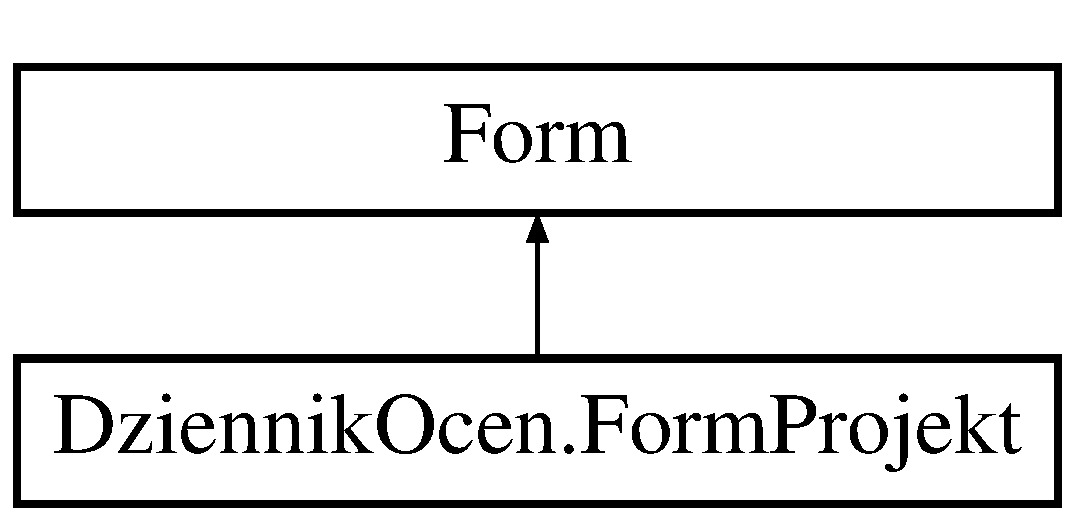
\includegraphics[height=2.000000cm]{class_dziennik_ocen_1_1_form_projekt}
\end{center}
\end{figure}
\subsection*{Public Member Functions}
\begin{DoxyCompactItemize}
\item 
\hyperlink{class_dziennik_ocen_1_1_form_projekt_a8be8499fb861f2375950c4e61e7dcc8a}{Form\+Projekt} (\hyperlink{class_dziennik_ocen_1_1_p_r_o_j_e_k_t}{P\+R\+O\+J\+E\+KT} \hyperlink{class_dziennik_ocen_1_1_form_projekt_a67e21510e269671aa133417cb9b111b5}{projekt}, I\+List$<$ \hyperlink{class_dziennik_ocen_1_1_p_r_z_e_d_m_i_o_t}{P\+R\+Z\+E\+D\+M\+I\+OT} $>$ przedmiot, int id)
\end{DoxyCompactItemize}
\subsection*{Protected Member Functions}
\begin{DoxyCompactItemize}
\item 
override void \hyperlink{class_dziennik_ocen_1_1_form_projekt_a78ce43373f97d5189228be2bd0a986db}{Dispose} (bool disposing)
\begin{DoxyCompactList}\small\item\em Clean up any resources being used. \end{DoxyCompactList}\end{DoxyCompactItemize}
\subsection*{Properties}
\begin{DoxyCompactItemize}
\item 
\hyperlink{class_dziennik_ocen_1_1_p_r_o_j_e_k_t}{P\+R\+O\+J\+E\+KT} \hyperlink{class_dziennik_ocen_1_1_form_projekt_a3fa55e05e8e5a170bb01eb7a0682a342}{Projekt}\hspace{0.3cm}{\ttfamily  \mbox{[}get, set\mbox{]}}
\end{DoxyCompactItemize}
\subsection*{Private Member Functions}
\begin{DoxyCompactItemize}
\item 
void \hyperlink{class_dziennik_ocen_1_1_form_projekt_af5c591d1f084dde2ea7389a669882a57}{btn\+Zapisz\+\_\+\+Click} (object sender, Event\+Args e)
\item 
void \hyperlink{class_dziennik_ocen_1_1_form_projekt_a17fb1a9c33ba3c82ea1f93b9c7dceb7d}{Initialize\+Component} ()
\begin{DoxyCompactList}\small\item\em Required method for Designer support -\/ do not modify the contents of this method with the code editor. \end{DoxyCompactList}\end{DoxyCompactItemize}
\subsection*{Private Attributes}
\begin{DoxyCompactItemize}
\item 
\hyperlink{class_dziennik_ocen_1_1_p_r_o_j_e_k_t}{P\+R\+O\+J\+E\+KT} \hyperlink{class_dziennik_ocen_1_1_form_projekt_a67e21510e269671aa133417cb9b111b5}{projekt}
\item 
\hyperlink{class_dziennik_ocen_1_1_dziennik_ocen_entities}{Dziennik\+Ocen\+Entities} \hyperlink{class_dziennik_ocen_1_1_form_projekt_a101debfea501b130728811f5ee73f415}{db} = new \hyperlink{class_dziennik_ocen_1_1_dziennik_ocen_entities}{Dziennik\+Ocen\+Entities}()
\item 
\hyperlink{class_dziennik_ocen_1_1_p_r_z_e_d_m_i_o_t}{P\+R\+Z\+E\+D\+M\+I\+OT} \hyperlink{class_dziennik_ocen_1_1_form_projekt_acd30f5e99c7bfb0323343e82c63d1402}{Wybrany\+Przedmiot}
\item 
System.\+Component\+Model.\+I\+Container \hyperlink{class_dziennik_ocen_1_1_form_projekt_a26a32516eb0f6b9653a1146f3f29a508}{components} = null
\begin{DoxyCompactList}\small\item\em Required designer variable. \end{DoxyCompactList}\item 
System.\+Windows.\+Forms.\+Text\+Box \hyperlink{class_dziennik_ocen_1_1_form_projekt_a0d6905e62e6aaee937d2ac06cc7d1eb9}{tbx\+Nazwa\+Projektu}
\item 
System.\+Windows.\+Forms.\+Text\+Box \hyperlink{class_dziennik_ocen_1_1_form_projekt_a60d556129867f1fc819674f0a06419f3}{tbx\+Opis\+Projektu}
\item 
System.\+Windows.\+Forms.\+Label \hyperlink{class_dziennik_ocen_1_1_form_projekt_a90aa6092eacccd1b59a8bb49483e3296}{lblnazwaprojektu}
\item 
System.\+Windows.\+Forms.\+Label \hyperlink{class_dziennik_ocen_1_1_form_projekt_a42e7b5a957cabfffba8283926174edf4}{lblopisprojektu}
\item 
System.\+Windows.\+Forms.\+Button \hyperlink{class_dziennik_ocen_1_1_form_projekt_af6063055927dff58ceed268ae1fbfbe6}{btn\+Zapisz}
\item 
System.\+Windows.\+Forms.\+Button \hyperlink{class_dziennik_ocen_1_1_form_projekt_a7d9e4b326ea8c5f943db124d9c10a52d}{btn\+Anuluj}
\item 
System.\+Windows.\+Forms.\+Combo\+Box \hyperlink{class_dziennik_ocen_1_1_form_projekt_af9c3f48763789fdf806504520036b588}{combo\+Box1}
\item 
System.\+Windows.\+Forms.\+Binding\+Source \hyperlink{class_dziennik_ocen_1_1_form_projekt_a3809e13068b772ca98649868e729a1af}{bs\+Przedmioty}
\item 
System.\+Windows.\+Forms.\+Label \hyperlink{class_dziennik_ocen_1_1_form_projekt_a4b417edd61727b2a6cfbffdfc0683735}{lbl\+Przedmiot}
\end{DoxyCompactItemize}


\subsection{Constructor \& Destructor Documentation}
\mbox{\Hypertarget{class_dziennik_ocen_1_1_form_projekt_a8be8499fb861f2375950c4e61e7dcc8a}\label{class_dziennik_ocen_1_1_form_projekt_a8be8499fb861f2375950c4e61e7dcc8a}} 
\index{Dziennik\+Ocen\+::\+Form\+Projekt@{Dziennik\+Ocen\+::\+Form\+Projekt}!Form\+Projekt@{Form\+Projekt}}
\index{Form\+Projekt@{Form\+Projekt}!Dziennik\+Ocen\+::\+Form\+Projekt@{Dziennik\+Ocen\+::\+Form\+Projekt}}
\subsubsection{\texorpdfstring{Form\+Projekt()}{FormProjekt()}}
{\footnotesize\ttfamily Dziennik\+Ocen.\+Form\+Projekt.\+Form\+Projekt (\begin{DoxyParamCaption}\item[{\hyperlink{class_dziennik_ocen_1_1_p_r_o_j_e_k_t}{P\+R\+O\+J\+E\+KT}}]{projekt,  }\item[{I\+List$<$ \hyperlink{class_dziennik_ocen_1_1_p_r_z_e_d_m_i_o_t}{P\+R\+Z\+E\+D\+M\+I\+OT} $>$}]{przedmiot,  }\item[{int}]{id }\end{DoxyParamCaption})\hspace{0.3cm}{\ttfamily [inline]}}



\subsection{Member Function Documentation}
\mbox{\Hypertarget{class_dziennik_ocen_1_1_form_projekt_af5c591d1f084dde2ea7389a669882a57}\label{class_dziennik_ocen_1_1_form_projekt_af5c591d1f084dde2ea7389a669882a57}} 
\index{Dziennik\+Ocen\+::\+Form\+Projekt@{Dziennik\+Ocen\+::\+Form\+Projekt}!btn\+Zapisz\+\_\+\+Click@{btn\+Zapisz\+\_\+\+Click}}
\index{btn\+Zapisz\+\_\+\+Click@{btn\+Zapisz\+\_\+\+Click}!Dziennik\+Ocen\+::\+Form\+Projekt@{Dziennik\+Ocen\+::\+Form\+Projekt}}
\subsubsection{\texorpdfstring{btn\+Zapisz\+\_\+\+Click()}{btnZapisz\_Click()}}
{\footnotesize\ttfamily void Dziennik\+Ocen.\+Form\+Projekt.\+btn\+Zapisz\+\_\+\+Click (\begin{DoxyParamCaption}\item[{object}]{sender,  }\item[{Event\+Args}]{e }\end{DoxyParamCaption})\hspace{0.3cm}{\ttfamily [inline]}, {\ttfamily [private]}}

\mbox{\Hypertarget{class_dziennik_ocen_1_1_form_projekt_a78ce43373f97d5189228be2bd0a986db}\label{class_dziennik_ocen_1_1_form_projekt_a78ce43373f97d5189228be2bd0a986db}} 
\index{Dziennik\+Ocen\+::\+Form\+Projekt@{Dziennik\+Ocen\+::\+Form\+Projekt}!Dispose@{Dispose}}
\index{Dispose@{Dispose}!Dziennik\+Ocen\+::\+Form\+Projekt@{Dziennik\+Ocen\+::\+Form\+Projekt}}
\subsubsection{\texorpdfstring{Dispose()}{Dispose()}}
{\footnotesize\ttfamily override void Dziennik\+Ocen.\+Form\+Projekt.\+Dispose (\begin{DoxyParamCaption}\item[{bool}]{disposing }\end{DoxyParamCaption})\hspace{0.3cm}{\ttfamily [inline]}, {\ttfamily [protected]}}



Clean up any resources being used. 


\begin{DoxyParams}{Parameters}
{\em disposing} & true if managed resources should be disposed; otherwise, false.\\
\hline
\end{DoxyParams}
\mbox{\Hypertarget{class_dziennik_ocen_1_1_form_projekt_a17fb1a9c33ba3c82ea1f93b9c7dceb7d}\label{class_dziennik_ocen_1_1_form_projekt_a17fb1a9c33ba3c82ea1f93b9c7dceb7d}} 
\index{Dziennik\+Ocen\+::\+Form\+Projekt@{Dziennik\+Ocen\+::\+Form\+Projekt}!Initialize\+Component@{Initialize\+Component}}
\index{Initialize\+Component@{Initialize\+Component}!Dziennik\+Ocen\+::\+Form\+Projekt@{Dziennik\+Ocen\+::\+Form\+Projekt}}
\subsubsection{\texorpdfstring{Initialize\+Component()}{InitializeComponent()}}
{\footnotesize\ttfamily void Dziennik\+Ocen.\+Form\+Projekt.\+Initialize\+Component (\begin{DoxyParamCaption}{ }\end{DoxyParamCaption})\hspace{0.3cm}{\ttfamily [inline]}, {\ttfamily [private]}}



Required method for Designer support -\/ do not modify the contents of this method with the code editor. 



\subsection{Member Data Documentation}
\mbox{\Hypertarget{class_dziennik_ocen_1_1_form_projekt_a3809e13068b772ca98649868e729a1af}\label{class_dziennik_ocen_1_1_form_projekt_a3809e13068b772ca98649868e729a1af}} 
\index{Dziennik\+Ocen\+::\+Form\+Projekt@{Dziennik\+Ocen\+::\+Form\+Projekt}!bs\+Przedmioty@{bs\+Przedmioty}}
\index{bs\+Przedmioty@{bs\+Przedmioty}!Dziennik\+Ocen\+::\+Form\+Projekt@{Dziennik\+Ocen\+::\+Form\+Projekt}}
\subsubsection{\texorpdfstring{bs\+Przedmioty}{bsPrzedmioty}}
{\footnotesize\ttfamily System.\+Windows.\+Forms.\+Binding\+Source Dziennik\+Ocen.\+Form\+Projekt.\+bs\+Przedmioty\hspace{0.3cm}{\ttfamily [private]}}

\mbox{\Hypertarget{class_dziennik_ocen_1_1_form_projekt_a7d9e4b326ea8c5f943db124d9c10a52d}\label{class_dziennik_ocen_1_1_form_projekt_a7d9e4b326ea8c5f943db124d9c10a52d}} 
\index{Dziennik\+Ocen\+::\+Form\+Projekt@{Dziennik\+Ocen\+::\+Form\+Projekt}!btn\+Anuluj@{btn\+Anuluj}}
\index{btn\+Anuluj@{btn\+Anuluj}!Dziennik\+Ocen\+::\+Form\+Projekt@{Dziennik\+Ocen\+::\+Form\+Projekt}}
\subsubsection{\texorpdfstring{btn\+Anuluj}{btnAnuluj}}
{\footnotesize\ttfamily System.\+Windows.\+Forms.\+Button Dziennik\+Ocen.\+Form\+Projekt.\+btn\+Anuluj\hspace{0.3cm}{\ttfamily [private]}}

\mbox{\Hypertarget{class_dziennik_ocen_1_1_form_projekt_af6063055927dff58ceed268ae1fbfbe6}\label{class_dziennik_ocen_1_1_form_projekt_af6063055927dff58ceed268ae1fbfbe6}} 
\index{Dziennik\+Ocen\+::\+Form\+Projekt@{Dziennik\+Ocen\+::\+Form\+Projekt}!btn\+Zapisz@{btn\+Zapisz}}
\index{btn\+Zapisz@{btn\+Zapisz}!Dziennik\+Ocen\+::\+Form\+Projekt@{Dziennik\+Ocen\+::\+Form\+Projekt}}
\subsubsection{\texorpdfstring{btn\+Zapisz}{btnZapisz}}
{\footnotesize\ttfamily System.\+Windows.\+Forms.\+Button Dziennik\+Ocen.\+Form\+Projekt.\+btn\+Zapisz\hspace{0.3cm}{\ttfamily [private]}}

\mbox{\Hypertarget{class_dziennik_ocen_1_1_form_projekt_af9c3f48763789fdf806504520036b588}\label{class_dziennik_ocen_1_1_form_projekt_af9c3f48763789fdf806504520036b588}} 
\index{Dziennik\+Ocen\+::\+Form\+Projekt@{Dziennik\+Ocen\+::\+Form\+Projekt}!combo\+Box1@{combo\+Box1}}
\index{combo\+Box1@{combo\+Box1}!Dziennik\+Ocen\+::\+Form\+Projekt@{Dziennik\+Ocen\+::\+Form\+Projekt}}
\subsubsection{\texorpdfstring{combo\+Box1}{comboBox1}}
{\footnotesize\ttfamily System.\+Windows.\+Forms.\+Combo\+Box Dziennik\+Ocen.\+Form\+Projekt.\+combo\+Box1\hspace{0.3cm}{\ttfamily [private]}}

\mbox{\Hypertarget{class_dziennik_ocen_1_1_form_projekt_a26a32516eb0f6b9653a1146f3f29a508}\label{class_dziennik_ocen_1_1_form_projekt_a26a32516eb0f6b9653a1146f3f29a508}} 
\index{Dziennik\+Ocen\+::\+Form\+Projekt@{Dziennik\+Ocen\+::\+Form\+Projekt}!components@{components}}
\index{components@{components}!Dziennik\+Ocen\+::\+Form\+Projekt@{Dziennik\+Ocen\+::\+Form\+Projekt}}
\subsubsection{\texorpdfstring{components}{components}}
{\footnotesize\ttfamily System.\+Component\+Model.\+I\+Container Dziennik\+Ocen.\+Form\+Projekt.\+components = null\hspace{0.3cm}{\ttfamily [private]}}



Required designer variable. 

\mbox{\Hypertarget{class_dziennik_ocen_1_1_form_projekt_a101debfea501b130728811f5ee73f415}\label{class_dziennik_ocen_1_1_form_projekt_a101debfea501b130728811f5ee73f415}} 
\index{Dziennik\+Ocen\+::\+Form\+Projekt@{Dziennik\+Ocen\+::\+Form\+Projekt}!db@{db}}
\index{db@{db}!Dziennik\+Ocen\+::\+Form\+Projekt@{Dziennik\+Ocen\+::\+Form\+Projekt}}
\subsubsection{\texorpdfstring{db}{db}}
{\footnotesize\ttfamily \hyperlink{class_dziennik_ocen_1_1_dziennik_ocen_entities}{Dziennik\+Ocen\+Entities} Dziennik\+Ocen.\+Form\+Projekt.\+db = new \hyperlink{class_dziennik_ocen_1_1_dziennik_ocen_entities}{Dziennik\+Ocen\+Entities}()\hspace{0.3cm}{\ttfamily [private]}}

\mbox{\Hypertarget{class_dziennik_ocen_1_1_form_projekt_a90aa6092eacccd1b59a8bb49483e3296}\label{class_dziennik_ocen_1_1_form_projekt_a90aa6092eacccd1b59a8bb49483e3296}} 
\index{Dziennik\+Ocen\+::\+Form\+Projekt@{Dziennik\+Ocen\+::\+Form\+Projekt}!lblnazwaprojektu@{lblnazwaprojektu}}
\index{lblnazwaprojektu@{lblnazwaprojektu}!Dziennik\+Ocen\+::\+Form\+Projekt@{Dziennik\+Ocen\+::\+Form\+Projekt}}
\subsubsection{\texorpdfstring{lblnazwaprojektu}{lblnazwaprojektu}}
{\footnotesize\ttfamily System.\+Windows.\+Forms.\+Label Dziennik\+Ocen.\+Form\+Projekt.\+lblnazwaprojektu\hspace{0.3cm}{\ttfamily [private]}}

\mbox{\Hypertarget{class_dziennik_ocen_1_1_form_projekt_a42e7b5a957cabfffba8283926174edf4}\label{class_dziennik_ocen_1_1_form_projekt_a42e7b5a957cabfffba8283926174edf4}} 
\index{Dziennik\+Ocen\+::\+Form\+Projekt@{Dziennik\+Ocen\+::\+Form\+Projekt}!lblopisprojektu@{lblopisprojektu}}
\index{lblopisprojektu@{lblopisprojektu}!Dziennik\+Ocen\+::\+Form\+Projekt@{Dziennik\+Ocen\+::\+Form\+Projekt}}
\subsubsection{\texorpdfstring{lblopisprojektu}{lblopisprojektu}}
{\footnotesize\ttfamily System.\+Windows.\+Forms.\+Label Dziennik\+Ocen.\+Form\+Projekt.\+lblopisprojektu\hspace{0.3cm}{\ttfamily [private]}}

\mbox{\Hypertarget{class_dziennik_ocen_1_1_form_projekt_a4b417edd61727b2a6cfbffdfc0683735}\label{class_dziennik_ocen_1_1_form_projekt_a4b417edd61727b2a6cfbffdfc0683735}} 
\index{Dziennik\+Ocen\+::\+Form\+Projekt@{Dziennik\+Ocen\+::\+Form\+Projekt}!lbl\+Przedmiot@{lbl\+Przedmiot}}
\index{lbl\+Przedmiot@{lbl\+Przedmiot}!Dziennik\+Ocen\+::\+Form\+Projekt@{Dziennik\+Ocen\+::\+Form\+Projekt}}
\subsubsection{\texorpdfstring{lbl\+Przedmiot}{lblPrzedmiot}}
{\footnotesize\ttfamily System.\+Windows.\+Forms.\+Label Dziennik\+Ocen.\+Form\+Projekt.\+lbl\+Przedmiot\hspace{0.3cm}{\ttfamily [private]}}

\mbox{\Hypertarget{class_dziennik_ocen_1_1_form_projekt_a67e21510e269671aa133417cb9b111b5}\label{class_dziennik_ocen_1_1_form_projekt_a67e21510e269671aa133417cb9b111b5}} 
\index{Dziennik\+Ocen\+::\+Form\+Projekt@{Dziennik\+Ocen\+::\+Form\+Projekt}!projekt@{projekt}}
\index{projekt@{projekt}!Dziennik\+Ocen\+::\+Form\+Projekt@{Dziennik\+Ocen\+::\+Form\+Projekt}}
\subsubsection{\texorpdfstring{projekt}{projekt}}
{\footnotesize\ttfamily \hyperlink{class_dziennik_ocen_1_1_p_r_o_j_e_k_t}{P\+R\+O\+J\+E\+KT} Dziennik\+Ocen.\+Form\+Projekt.\+projekt\hspace{0.3cm}{\ttfamily [private]}}

\mbox{\Hypertarget{class_dziennik_ocen_1_1_form_projekt_a0d6905e62e6aaee937d2ac06cc7d1eb9}\label{class_dziennik_ocen_1_1_form_projekt_a0d6905e62e6aaee937d2ac06cc7d1eb9}} 
\index{Dziennik\+Ocen\+::\+Form\+Projekt@{Dziennik\+Ocen\+::\+Form\+Projekt}!tbx\+Nazwa\+Projektu@{tbx\+Nazwa\+Projektu}}
\index{tbx\+Nazwa\+Projektu@{tbx\+Nazwa\+Projektu}!Dziennik\+Ocen\+::\+Form\+Projekt@{Dziennik\+Ocen\+::\+Form\+Projekt}}
\subsubsection{\texorpdfstring{tbx\+Nazwa\+Projektu}{tbxNazwaProjektu}}
{\footnotesize\ttfamily System.\+Windows.\+Forms.\+Text\+Box Dziennik\+Ocen.\+Form\+Projekt.\+tbx\+Nazwa\+Projektu\hspace{0.3cm}{\ttfamily [private]}}

\mbox{\Hypertarget{class_dziennik_ocen_1_1_form_projekt_a60d556129867f1fc819674f0a06419f3}\label{class_dziennik_ocen_1_1_form_projekt_a60d556129867f1fc819674f0a06419f3}} 
\index{Dziennik\+Ocen\+::\+Form\+Projekt@{Dziennik\+Ocen\+::\+Form\+Projekt}!tbx\+Opis\+Projektu@{tbx\+Opis\+Projektu}}
\index{tbx\+Opis\+Projektu@{tbx\+Opis\+Projektu}!Dziennik\+Ocen\+::\+Form\+Projekt@{Dziennik\+Ocen\+::\+Form\+Projekt}}
\subsubsection{\texorpdfstring{tbx\+Opis\+Projektu}{tbxOpisProjektu}}
{\footnotesize\ttfamily System.\+Windows.\+Forms.\+Text\+Box Dziennik\+Ocen.\+Form\+Projekt.\+tbx\+Opis\+Projektu\hspace{0.3cm}{\ttfamily [private]}}

\mbox{\Hypertarget{class_dziennik_ocen_1_1_form_projekt_acd30f5e99c7bfb0323343e82c63d1402}\label{class_dziennik_ocen_1_1_form_projekt_acd30f5e99c7bfb0323343e82c63d1402}} 
\index{Dziennik\+Ocen\+::\+Form\+Projekt@{Dziennik\+Ocen\+::\+Form\+Projekt}!Wybrany\+Przedmiot@{Wybrany\+Przedmiot}}
\index{Wybrany\+Przedmiot@{Wybrany\+Przedmiot}!Dziennik\+Ocen\+::\+Form\+Projekt@{Dziennik\+Ocen\+::\+Form\+Projekt}}
\subsubsection{\texorpdfstring{Wybrany\+Przedmiot}{WybranyPrzedmiot}}
{\footnotesize\ttfamily \hyperlink{class_dziennik_ocen_1_1_p_r_z_e_d_m_i_o_t}{P\+R\+Z\+E\+D\+M\+I\+OT} Dziennik\+Ocen.\+Form\+Projekt.\+Wybrany\+Przedmiot\hspace{0.3cm}{\ttfamily [private]}}



\subsection{Property Documentation}
\mbox{\Hypertarget{class_dziennik_ocen_1_1_form_projekt_a3fa55e05e8e5a170bb01eb7a0682a342}\label{class_dziennik_ocen_1_1_form_projekt_a3fa55e05e8e5a170bb01eb7a0682a342}} 
\index{Dziennik\+Ocen\+::\+Form\+Projekt@{Dziennik\+Ocen\+::\+Form\+Projekt}!Projekt@{Projekt}}
\index{Projekt@{Projekt}!Dziennik\+Ocen\+::\+Form\+Projekt@{Dziennik\+Ocen\+::\+Form\+Projekt}}
\subsubsection{\texorpdfstring{Projekt}{Projekt}}
{\footnotesize\ttfamily \hyperlink{class_dziennik_ocen_1_1_p_r_o_j_e_k_t}{P\+R\+O\+J\+E\+KT} Dziennik\+Ocen.\+Form\+Projekt.\+Projekt\hspace{0.3cm}{\ttfamily [get]}, {\ttfamily [set]}}



The documentation for this class was generated from the following files\+:\begin{DoxyCompactItemize}
\item 
Dziennik\+Ocen/\hyperlink{_form_projekt_8cs}{Form\+Projekt.\+cs}\item 
Dziennik\+Ocen/\hyperlink{_form_projekt_8_designer_8cs}{Form\+Projekt.\+Designer.\+cs}\end{DoxyCompactItemize}

\hypertarget{class_dziennik_ocen_1_1_form_prowadzacy}{}\section{Dziennik\+Ocen.\+Form\+Prowadzacy Class Reference}
\label{class_dziennik_ocen_1_1_form_prowadzacy}\index{Dziennik\+Ocen.\+Form\+Prowadzacy@{Dziennik\+Ocen.\+Form\+Prowadzacy}}
Inheritance diagram for Dziennik\+Ocen.\+Form\+Prowadzacy\+:\begin{figure}[H]
\begin{center}
\leavevmode
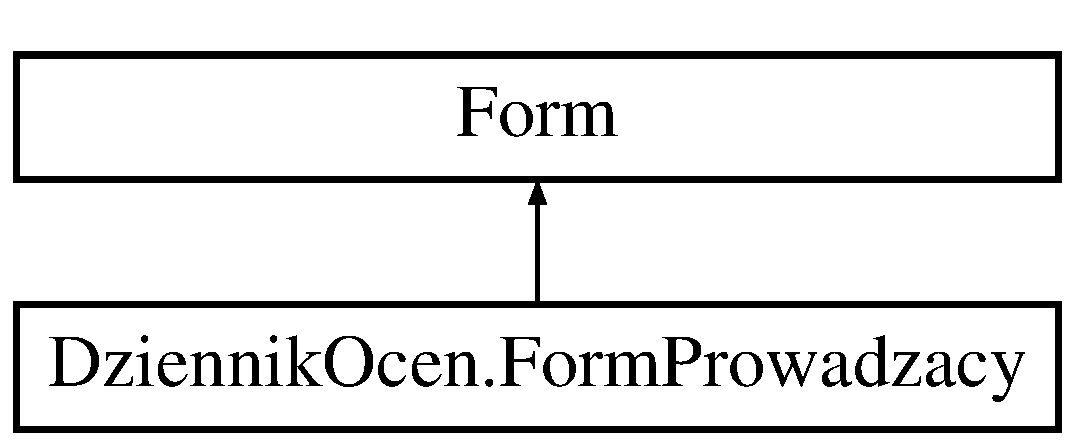
\includegraphics[height=2.000000cm]{class_dziennik_ocen_1_1_form_prowadzacy}
\end{center}
\end{figure}
\subsection*{Public Member Functions}
\begin{DoxyCompactItemize}
\item 
\hyperlink{class_dziennik_ocen_1_1_form_prowadzacy_a3b383a27c47250980feb63495b1e06a6}{Form\+Prowadzacy} (string \hyperlink{class_dziennik_ocen_1_1_form_prowadzacy_a2a8c88aed0e523c43b18ac50002680d4}{Email}, string \hyperlink{class_dziennik_ocen_1_1_form_prowadzacy_a97552a9d67d35422ddc14b94222d100b}{Haslo})
\item 
\hyperlink{class_dziennik_ocen_1_1projekty}{projekty} \hyperlink{class_dziennik_ocen_1_1_form_prowadzacy_ab1f0a40f408e000fc15acafed5910bce}{Znajdz\+Projekt} (int id, int idst)
\item 
\hyperlink{class_dziennik_ocen_1_1_p_r_o_w_a_d_z_xC4_x84_c_y}{P\+R\+O\+W\+A\+D\+ZĄ\+CY} \hyperlink{class_dziennik_ocen_1_1_form_prowadzacy_a1836411433e5b2c6dd8b85e9df9c46d0}{Znajdz\+Prowadzacego} (string \hyperlink{class_dziennik_ocen_1_1_form_prowadzacy_a2a8c88aed0e523c43b18ac50002680d4}{Email}, string \hyperlink{class_dziennik_ocen_1_1_form_prowadzacy_a97552a9d67d35422ddc14b94222d100b}{Haslo})
\end{DoxyCompactItemize}
\subsection*{Protected Member Functions}
\begin{DoxyCompactItemize}
\item 
override void \hyperlink{class_dziennik_ocen_1_1_form_prowadzacy_a33b9f735dca4c248819321d0692c98c5}{Dispose} (bool disposing)
\begin{DoxyCompactList}\small\item\em Clean up any resources being used. \end{DoxyCompactList}\end{DoxyCompactItemize}
\subsection*{Properties}
\begin{DoxyCompactItemize}
\item 
\hyperlink{class_dziennik_ocen_1_1_s_t_u_d_e_n_t}{S\+T\+U\+D\+E\+NT} \hyperlink{class_dziennik_ocen_1_1_form_prowadzacy_affdca976e8a2ca32c6aef4f70a7996d2}{Aktualnie\+Zaznaczony\+Student}\hspace{0.3cm}{\ttfamily  \mbox{[}get\mbox{]}}
\item 
\hyperlink{class_dziennik_ocen_1_1_p_r_o_j_e_k_t}{P\+R\+O\+J\+E\+KT} \hyperlink{class_dziennik_ocen_1_1_form_prowadzacy_adf43b053c3531f1dc0a758e08a282955}{Aktualnie\+Zaznaczony\+Projekt}\hspace{0.3cm}{\ttfamily  \mbox{[}get\mbox{]}}
\end{DoxyCompactItemize}
\subsection*{Private Member Functions}
\begin{DoxyCompactItemize}
\item 
void \hyperlink{class_dziennik_ocen_1_1_form_prowadzacy_a2bdcad4bb383eb56ae128ead097862e1}{Zaladuj\+Studentow} ()
\item 
void \hyperlink{class_dziennik_ocen_1_1_form_prowadzacy_a27f7245c5c86426b35219a4d0850a05c}{Zaladuj\+Projekty} ()
\item 
void \hyperlink{class_dziennik_ocen_1_1_form_prowadzacy_a2f8bd99711e10fb18c776dc5ec5ec171}{studenci\+Tool\+Strip\+Menu\+Item\+\_\+\+Click} (object sender, Event\+Args e)
\item 
void \hyperlink{class_dziennik_ocen_1_1_form_prowadzacy_a695f645edeabba811779292326e73f02}{Zaladuj\+Projekty} (\hyperlink{class_dziennik_ocen_1_1_s_t_u_d_e_n_t}{S\+T\+U\+D\+E\+NT} \hyperlink{class_dziennik_ocen_1_1_form_prowadzacy_affdca976e8a2ca32c6aef4f70a7996d2}{Aktualnie\+Zaznaczony\+Student})
\item 
void \hyperlink{class_dziennik_ocen_1_1_form_prowadzacy_aae16e5755cb4132cbb941210b73c718d}{btn\+Dodaj\+Studenta\+\_\+\+Click} (object sender, Event\+Args e)
\item 
void \hyperlink{class_dziennik_ocen_1_1_form_prowadzacy_a3aa4601472caec2e4a272b7dc3547e48}{btn\+Edytuj\+Studenta\+\_\+\+Click} (object sender, Event\+Args e)
\item 
void \hyperlink{class_dziennik_ocen_1_1_form_prowadzacy_acceb0ccd4975fe46741d9bdaeb35f469}{btn\+Usun\+Projekt\+\_\+\+Click} (object sender, Event\+Args e)
\item 
void \hyperlink{class_dziennik_ocen_1_1_form_prowadzacy_abfdb2dee5763c253e7ec32de21df53d5}{Form\+Prowadzacy\+\_\+\+Form\+Closing} (object sender, Form\+Closing\+Event\+Args e)
\item 
void \hyperlink{class_dziennik_ocen_1_1_form_prowadzacy_a69445c06a27fa8a0ccafdcdef9f18d52}{projekty\+Tool\+Strip\+Menu\+Item\+\_\+\+Click} (object sender, Event\+Args e)
\item 
void \hyperlink{class_dziennik_ocen_1_1_form_prowadzacy_adcbaca064b616975dc51a2893d0304bd}{btn\+Dodaj\+Projektt\+\_\+\+Click} (object sender, Event\+Args e)
\item 
void \hyperlink{class_dziennik_ocen_1_1_form_prowadzacy_ab6aa86c1bebee342ca89aca35b0d6330}{btn\+Edytuj\+Projektt\+\_\+\+Click} (object sender, Event\+Args e)
\item 
void \hyperlink{class_dziennik_ocen_1_1_form_prowadzacy_abd8f5d37f95c980ea2d993ff2fdaac55}{btn\+Usun\+Projektt\+\_\+\+Click} (object sender, Event\+Args e)
\item 
void \hyperlink{class_dziennik_ocen_1_1_form_prowadzacy_aadb5dd637e2bea7b63d69e16a8ee8c50}{btn\+Usun\+Studenta\+\_\+\+Click} (object sender, Event\+Args e)
\item 
void \hyperlink{class_dziennik_ocen_1_1_form_prowadzacy_a3947fae964426bffb87f3dde229681f4}{dgv\+Studenci\+Projekty\+\_\+\+Selection\+Changed} (object sender, Event\+Args e)
\item 
void \hyperlink{class_dziennik_ocen_1_1_form_prowadzacy_acbf83dbd039b578f4e66d933668f50f1}{dgv\+Studenci\+\_\+\+Mouse\+Click} (object sender, Mouse\+Event\+Args e)
\item 
void \hyperlink{class_dziennik_ocen_1_1_form_prowadzacy_a74ec7d96eb8beeaddad0fed8f7fcbc8c}{btn\+Edytuj\+Projekt\+\_\+\+Click} (object sender, Event\+Args e)
\item 
void \hyperlink{class_dziennik_ocen_1_1_form_prowadzacy_a94e3e380b95874b6f037c44d2d514677}{Initialize\+Component} ()
\begin{DoxyCompactList}\small\item\em Required method for Designer support -\/ do not modify the contents of this method with the code editor. \end{DoxyCompactList}\end{DoxyCompactItemize}
\subsection*{Private Attributes}
\begin{DoxyCompactItemize}
\item 
\hyperlink{class_dziennik_ocen_1_1_dziennik_ocen_entities}{Dziennik\+Ocen\+Entities} \hyperlink{class_dziennik_ocen_1_1_form_prowadzacy_a8debab90e31034998329165c00836aca}{db} = new \hyperlink{class_dziennik_ocen_1_1_dziennik_ocen_entities}{Dziennik\+Ocen\+Entities}()
\item 
\hyperlink{class_dziennik_ocen_1_1_p_r_o_w_a_d_z_xC4_x84_c_y}{P\+R\+O\+W\+A\+D\+ZĄ\+CY} \hyperlink{class_dziennik_ocen_1_1_form_prowadzacy_a36367f60833c5ef9928db605143c1f9b}{zalogowany}
\item 
String \hyperlink{class_dziennik_ocen_1_1_form_prowadzacy_a152e43d7b72d76a06fdea70f0aaf92e5}{String\+\_\+imie\+\_\+prowadzacego}
\item 
String \hyperlink{class_dziennik_ocen_1_1_form_prowadzacy_afd2e14b9219c1568b3b06ec1131b1256}{String\+\_\+nazwisko\+\_\+prowadzacego}
\item 
String \hyperlink{class_dziennik_ocen_1_1_form_prowadzacy_afe096a0f8d35718d3971c19359d3674c}{String\+\_\+id\+\_\+projektu}
\item 
String \hyperlink{class_dziennik_ocen_1_1_form_prowadzacy_a2a8c88aed0e523c43b18ac50002680d4}{Email}
\item 
String \hyperlink{class_dziennik_ocen_1_1_form_prowadzacy_a97552a9d67d35422ddc14b94222d100b}{Haslo}
\item 
System.\+Component\+Model.\+I\+Container \hyperlink{class_dziennik_ocen_1_1_form_prowadzacy_a74ef1b6ab2d81abfa6a0f441ff9e8ec6}{components} = null
\begin{DoxyCompactList}\small\item\em Required designer variable. \end{DoxyCompactList}\item 
System.\+Windows.\+Forms.\+Menu\+Strip \hyperlink{class_dziennik_ocen_1_1_form_prowadzacy_ae5ef793320aa64d107281ca1e3254c50}{menu\+Strip1}
\item 
System.\+Windows.\+Forms.\+Tool\+Strip\+Menu\+Item \hyperlink{class_dziennik_ocen_1_1_form_prowadzacy_a220128b78996df92745a4945919daf9b}{studenci\+Tool\+Strip\+Menu\+Item}
\item 
System.\+Windows.\+Forms.\+Tool\+Strip\+Menu\+Item \hyperlink{class_dziennik_ocen_1_1_form_prowadzacy_a7c069bd9f8684667df3a89500f0cf02d}{projekty\+Tool\+Strip\+Menu\+Item}
\item 
System.\+Windows.\+Forms.\+Data\+Grid\+View \hyperlink{class_dziennik_ocen_1_1_form_prowadzacy_a280134b3087c1db583b6d8accdb11d73}{dgv\+Studenci}
\item 
System.\+Windows.\+Forms.\+Data\+Grid\+View \hyperlink{class_dziennik_ocen_1_1_form_prowadzacy_a20ff62aa8f7c123b9276bd6e133ff714}{dgv\+Studenci\+Projekty}
\item 
System.\+Windows.\+Forms.\+Binding\+Source \hyperlink{class_dziennik_ocen_1_1_form_prowadzacy_acb3d54ff7aa50085f771db31c0f485e0}{bs\+Studenci}
\item 
System.\+Windows.\+Forms.\+Data\+Grid\+View\+Text\+Box\+Column \hyperlink{class_dziennik_ocen_1_1_form_prowadzacy_a33dec2a21fdb11d452047f1afc2d8a96}{id\+S\+T\+U\+D\+E\+N\+T\+A\+Data\+Grid\+View\+Text\+Box\+Column}
\item 
System.\+Windows.\+Forms.\+Data\+Grid\+View\+Text\+Box\+Column \hyperlink{class_dziennik_ocen_1_1_form_prowadzacy_a15f429ca0f0961dd4571c63138da4a44}{id\+G\+R\+U\+P\+Y\+Data\+Grid\+View\+Text\+Box\+Column}
\item 
System.\+Windows.\+Forms.\+Data\+Grid\+View\+Text\+Box\+Column \hyperlink{class_dziennik_ocen_1_1_form_prowadzacy_a82220a781511306722d00a5bb8e34ba8}{imie\+Data\+Grid\+View\+Text\+Box\+Column}
\item 
System.\+Windows.\+Forms.\+Data\+Grid\+View\+Text\+Box\+Column \hyperlink{class_dziennik_ocen_1_1_form_prowadzacy_a55462891f1ebc82f3bd540a5ba7724d8}{nazwisko\+Data\+Grid\+View\+Text\+Box\+Column}
\item 
System.\+Windows.\+Forms.\+Data\+Grid\+View\+Text\+Box\+Column \hyperlink{class_dziennik_ocen_1_1_form_prowadzacy_a42c35ed0c3c7f4bf6d91cdcf8425ce5d}{telefon\+Data\+Grid\+View\+Text\+Box\+Column}
\item 
System.\+Windows.\+Forms.\+Data\+Grid\+View\+Text\+Box\+Column \hyperlink{class_dziennik_ocen_1_1_form_prowadzacy_a8f69f55632c9ef001cedd52d78e033e9}{adres\+Data\+Grid\+View\+Text\+Box\+Column}
\item 
System.\+Windows.\+Forms.\+Data\+Grid\+View\+Text\+Box\+Column \hyperlink{class_dziennik_ocen_1_1_form_prowadzacy_aac63cf038655c3c816becf4f3c877e21}{email\+Data\+Grid\+View\+Text\+Box\+Column}
\item 
System.\+Windows.\+Forms.\+Button \hyperlink{class_dziennik_ocen_1_1_form_prowadzacy_a2ba007452bcd972a9c6e27873e7ec9f2}{btn\+Dodaj\+Studenta}
\item 
System.\+Windows.\+Forms.\+Button \hyperlink{class_dziennik_ocen_1_1_form_prowadzacy_a9696c9b859ef8c8319cae4bbd11541bc}{btn\+Edytuj\+Studenta}
\item 
System.\+Windows.\+Forms.\+Button \hyperlink{class_dziennik_ocen_1_1_form_prowadzacy_a1e61eed4407829503f9bcaa236a7d090}{btn\+Usun\+Studenta}
\item 
System.\+Windows.\+Forms.\+Label \hyperlink{class_dziennik_ocen_1_1_form_prowadzacy_a72199d1fd316d587834235d3ad31b240}{label1}
\item 
System.\+Windows.\+Forms.\+Binding\+Source \hyperlink{class_dziennik_ocen_1_1_form_prowadzacy_a1e25c6eb9309cb7bbdd229cbaea7d961}{bs\+Projekty}
\item 
System.\+Windows.\+Forms.\+Label \hyperlink{class_dziennik_ocen_1_1_form_prowadzacy_a4dce4ea456be76f21fcb0f1b9b5c6518}{label2}
\item 
System.\+Windows.\+Forms.\+Button \hyperlink{class_dziennik_ocen_1_1_form_prowadzacy_aa6ac131a793db6be81f3009e17bdee95}{btn\+Usun\+Projekt}
\item 
System.\+Windows.\+Forms.\+Button \hyperlink{class_dziennik_ocen_1_1_form_prowadzacy_ae8a91b72998abe6cee9bd541b6853101}{btn\+Edytuj\+Projekt}
\item 
System.\+Windows.\+Forms.\+Binding\+Source \hyperlink{class_dziennik_ocen_1_1_form_prowadzacy_a94fe0aa43a553db5d96022e42ba299c4}{bsprojektyy}
\item 
System.\+Windows.\+Forms.\+Data\+Grid\+View \hyperlink{class_dziennik_ocen_1_1_form_prowadzacy_aa8ce9306108e10e546d2e0c858207127}{dgvprojekty}
\item 
System.\+Windows.\+Forms.\+Button \hyperlink{class_dziennik_ocen_1_1_form_prowadzacy_aa27cfc76b930c1647c3e0902ded456c7}{btn\+Dodaj\+Projektt}
\item 
System.\+Windows.\+Forms.\+Button \hyperlink{class_dziennik_ocen_1_1_form_prowadzacy_a490ebb19c58f7f4320806656cc8fcc5b}{btn\+Edytuj\+Projektt}
\item 
System.\+Windows.\+Forms.\+Button \hyperlink{class_dziennik_ocen_1_1_form_prowadzacy_ac0c4ae6f72bee4e9fbc5e35fea1c9a81}{btn\+Usun\+Projektt}
\item 
System.\+Windows.\+Forms.\+Label \hyperlink{class_dziennik_ocen_1_1_form_prowadzacy_a1ef7707072a50d4c7f268eab9ff86c30}{label3}
\item 
System.\+Windows.\+Forms.\+Data\+Grid\+View\+Text\+Box\+Column \hyperlink{class_dziennik_ocen_1_1_form_prowadzacy_a37cdef588a3d89e847669f80869e489c}{id\+P\+R\+O\+J\+E\+K\+T\+U\+Data\+Grid\+View\+Text\+Box\+Column}
\item 
System.\+Windows.\+Forms.\+Data\+Grid\+View\+Text\+Box\+Column \hyperlink{class_dziennik_ocen_1_1_form_prowadzacy_a2f3562d595efd99137a56d8297ce2e35}{id\+\_\+\+P\+R\+Z\+E\+D\+M\+I\+O\+TU}
\item 
System.\+Windows.\+Forms.\+Data\+Grid\+View\+Text\+Box\+Column \hyperlink{class_dziennik_ocen_1_1_form_prowadzacy_aa207a32efffe15f7ad829033a0a4d098}{nazwa\+\_\+projektu}
\item 
System.\+Windows.\+Forms.\+Data\+Grid\+View\+Text\+Box\+Column \hyperlink{class_dziennik_ocen_1_1_form_prowadzacy_ad49d1111a2fb6a998d55323e56dd5fe1}{opis\+\_\+projektu}
\item 
System.\+Windows.\+Forms.\+Data\+Grid\+View\+Text\+Box\+Column \hyperlink{class_dziennik_ocen_1_1_form_prowadzacy_a025edc876e60aa441df53b8a249f532e}{data\+Grid\+View\+Text\+Box\+Column1}
\end{DoxyCompactItemize}


\subsection{Constructor \& Destructor Documentation}
\mbox{\Hypertarget{class_dziennik_ocen_1_1_form_prowadzacy_a3b383a27c47250980feb63495b1e06a6}\label{class_dziennik_ocen_1_1_form_prowadzacy_a3b383a27c47250980feb63495b1e06a6}} 
\index{Dziennik\+Ocen\+::\+Form\+Prowadzacy@{Dziennik\+Ocen\+::\+Form\+Prowadzacy}!Form\+Prowadzacy@{Form\+Prowadzacy}}
\index{Form\+Prowadzacy@{Form\+Prowadzacy}!Dziennik\+Ocen\+::\+Form\+Prowadzacy@{Dziennik\+Ocen\+::\+Form\+Prowadzacy}}
\subsubsection{\texorpdfstring{Form\+Prowadzacy()}{FormProwadzacy()}}
{\footnotesize\ttfamily Dziennik\+Ocen.\+Form\+Prowadzacy.\+Form\+Prowadzacy (\begin{DoxyParamCaption}\item[{string}]{Email,  }\item[{string}]{Haslo }\end{DoxyParamCaption})\hspace{0.3cm}{\ttfamily [inline]}}



\subsection{Member Function Documentation}
\mbox{\Hypertarget{class_dziennik_ocen_1_1_form_prowadzacy_adcbaca064b616975dc51a2893d0304bd}\label{class_dziennik_ocen_1_1_form_prowadzacy_adcbaca064b616975dc51a2893d0304bd}} 
\index{Dziennik\+Ocen\+::\+Form\+Prowadzacy@{Dziennik\+Ocen\+::\+Form\+Prowadzacy}!btn\+Dodaj\+Projektt\+\_\+\+Click@{btn\+Dodaj\+Projektt\+\_\+\+Click}}
\index{btn\+Dodaj\+Projektt\+\_\+\+Click@{btn\+Dodaj\+Projektt\+\_\+\+Click}!Dziennik\+Ocen\+::\+Form\+Prowadzacy@{Dziennik\+Ocen\+::\+Form\+Prowadzacy}}
\subsubsection{\texorpdfstring{btn\+Dodaj\+Projektt\+\_\+\+Click()}{btnDodajProjektt\_Click()}}
{\footnotesize\ttfamily void Dziennik\+Ocen.\+Form\+Prowadzacy.\+btn\+Dodaj\+Projektt\+\_\+\+Click (\begin{DoxyParamCaption}\item[{object}]{sender,  }\item[{Event\+Args}]{e }\end{DoxyParamCaption})\hspace{0.3cm}{\ttfamily [inline]}, {\ttfamily [private]}}

\mbox{\Hypertarget{class_dziennik_ocen_1_1_form_prowadzacy_aae16e5755cb4132cbb941210b73c718d}\label{class_dziennik_ocen_1_1_form_prowadzacy_aae16e5755cb4132cbb941210b73c718d}} 
\index{Dziennik\+Ocen\+::\+Form\+Prowadzacy@{Dziennik\+Ocen\+::\+Form\+Prowadzacy}!btn\+Dodaj\+Studenta\+\_\+\+Click@{btn\+Dodaj\+Studenta\+\_\+\+Click}}
\index{btn\+Dodaj\+Studenta\+\_\+\+Click@{btn\+Dodaj\+Studenta\+\_\+\+Click}!Dziennik\+Ocen\+::\+Form\+Prowadzacy@{Dziennik\+Ocen\+::\+Form\+Prowadzacy}}
\subsubsection{\texorpdfstring{btn\+Dodaj\+Studenta\+\_\+\+Click()}{btnDodajStudenta\_Click()}}
{\footnotesize\ttfamily void Dziennik\+Ocen.\+Form\+Prowadzacy.\+btn\+Dodaj\+Studenta\+\_\+\+Click (\begin{DoxyParamCaption}\item[{object}]{sender,  }\item[{Event\+Args}]{e }\end{DoxyParamCaption})\hspace{0.3cm}{\ttfamily [inline]}, {\ttfamily [private]}}

\mbox{\Hypertarget{class_dziennik_ocen_1_1_form_prowadzacy_a74ec7d96eb8beeaddad0fed8f7fcbc8c}\label{class_dziennik_ocen_1_1_form_prowadzacy_a74ec7d96eb8beeaddad0fed8f7fcbc8c}} 
\index{Dziennik\+Ocen\+::\+Form\+Prowadzacy@{Dziennik\+Ocen\+::\+Form\+Prowadzacy}!btn\+Edytuj\+Projekt\+\_\+\+Click@{btn\+Edytuj\+Projekt\+\_\+\+Click}}
\index{btn\+Edytuj\+Projekt\+\_\+\+Click@{btn\+Edytuj\+Projekt\+\_\+\+Click}!Dziennik\+Ocen\+::\+Form\+Prowadzacy@{Dziennik\+Ocen\+::\+Form\+Prowadzacy}}
\subsubsection{\texorpdfstring{btn\+Edytuj\+Projekt\+\_\+\+Click()}{btnEdytujProjekt\_Click()}}
{\footnotesize\ttfamily void Dziennik\+Ocen.\+Form\+Prowadzacy.\+btn\+Edytuj\+Projekt\+\_\+\+Click (\begin{DoxyParamCaption}\item[{object}]{sender,  }\item[{Event\+Args}]{e }\end{DoxyParamCaption})\hspace{0.3cm}{\ttfamily [inline]}, {\ttfamily [private]}}

\mbox{\Hypertarget{class_dziennik_ocen_1_1_form_prowadzacy_ab6aa86c1bebee342ca89aca35b0d6330}\label{class_dziennik_ocen_1_1_form_prowadzacy_ab6aa86c1bebee342ca89aca35b0d6330}} 
\index{Dziennik\+Ocen\+::\+Form\+Prowadzacy@{Dziennik\+Ocen\+::\+Form\+Prowadzacy}!btn\+Edytuj\+Projektt\+\_\+\+Click@{btn\+Edytuj\+Projektt\+\_\+\+Click}}
\index{btn\+Edytuj\+Projektt\+\_\+\+Click@{btn\+Edytuj\+Projektt\+\_\+\+Click}!Dziennik\+Ocen\+::\+Form\+Prowadzacy@{Dziennik\+Ocen\+::\+Form\+Prowadzacy}}
\subsubsection{\texorpdfstring{btn\+Edytuj\+Projektt\+\_\+\+Click()}{btnEdytujProjektt\_Click()}}
{\footnotesize\ttfamily void Dziennik\+Ocen.\+Form\+Prowadzacy.\+btn\+Edytuj\+Projektt\+\_\+\+Click (\begin{DoxyParamCaption}\item[{object}]{sender,  }\item[{Event\+Args}]{e }\end{DoxyParamCaption})\hspace{0.3cm}{\ttfamily [inline]}, {\ttfamily [private]}}

\mbox{\Hypertarget{class_dziennik_ocen_1_1_form_prowadzacy_a3aa4601472caec2e4a272b7dc3547e48}\label{class_dziennik_ocen_1_1_form_prowadzacy_a3aa4601472caec2e4a272b7dc3547e48}} 
\index{Dziennik\+Ocen\+::\+Form\+Prowadzacy@{Dziennik\+Ocen\+::\+Form\+Prowadzacy}!btn\+Edytuj\+Studenta\+\_\+\+Click@{btn\+Edytuj\+Studenta\+\_\+\+Click}}
\index{btn\+Edytuj\+Studenta\+\_\+\+Click@{btn\+Edytuj\+Studenta\+\_\+\+Click}!Dziennik\+Ocen\+::\+Form\+Prowadzacy@{Dziennik\+Ocen\+::\+Form\+Prowadzacy}}
\subsubsection{\texorpdfstring{btn\+Edytuj\+Studenta\+\_\+\+Click()}{btnEdytujStudenta\_Click()}}
{\footnotesize\ttfamily void Dziennik\+Ocen.\+Form\+Prowadzacy.\+btn\+Edytuj\+Studenta\+\_\+\+Click (\begin{DoxyParamCaption}\item[{object}]{sender,  }\item[{Event\+Args}]{e }\end{DoxyParamCaption})\hspace{0.3cm}{\ttfamily [inline]}, {\ttfamily [private]}}

\mbox{\Hypertarget{class_dziennik_ocen_1_1_form_prowadzacy_acceb0ccd4975fe46741d9bdaeb35f469}\label{class_dziennik_ocen_1_1_form_prowadzacy_acceb0ccd4975fe46741d9bdaeb35f469}} 
\index{Dziennik\+Ocen\+::\+Form\+Prowadzacy@{Dziennik\+Ocen\+::\+Form\+Prowadzacy}!btn\+Usun\+Projekt\+\_\+\+Click@{btn\+Usun\+Projekt\+\_\+\+Click}}
\index{btn\+Usun\+Projekt\+\_\+\+Click@{btn\+Usun\+Projekt\+\_\+\+Click}!Dziennik\+Ocen\+::\+Form\+Prowadzacy@{Dziennik\+Ocen\+::\+Form\+Prowadzacy}}
\subsubsection{\texorpdfstring{btn\+Usun\+Projekt\+\_\+\+Click()}{btnUsunProjekt\_Click()}}
{\footnotesize\ttfamily void Dziennik\+Ocen.\+Form\+Prowadzacy.\+btn\+Usun\+Projekt\+\_\+\+Click (\begin{DoxyParamCaption}\item[{object}]{sender,  }\item[{Event\+Args}]{e }\end{DoxyParamCaption})\hspace{0.3cm}{\ttfamily [inline]}, {\ttfamily [private]}}

\mbox{\Hypertarget{class_dziennik_ocen_1_1_form_prowadzacy_abd8f5d37f95c980ea2d993ff2fdaac55}\label{class_dziennik_ocen_1_1_form_prowadzacy_abd8f5d37f95c980ea2d993ff2fdaac55}} 
\index{Dziennik\+Ocen\+::\+Form\+Prowadzacy@{Dziennik\+Ocen\+::\+Form\+Prowadzacy}!btn\+Usun\+Projektt\+\_\+\+Click@{btn\+Usun\+Projektt\+\_\+\+Click}}
\index{btn\+Usun\+Projektt\+\_\+\+Click@{btn\+Usun\+Projektt\+\_\+\+Click}!Dziennik\+Ocen\+::\+Form\+Prowadzacy@{Dziennik\+Ocen\+::\+Form\+Prowadzacy}}
\subsubsection{\texorpdfstring{btn\+Usun\+Projektt\+\_\+\+Click()}{btnUsunProjektt\_Click()}}
{\footnotesize\ttfamily void Dziennik\+Ocen.\+Form\+Prowadzacy.\+btn\+Usun\+Projektt\+\_\+\+Click (\begin{DoxyParamCaption}\item[{object}]{sender,  }\item[{Event\+Args}]{e }\end{DoxyParamCaption})\hspace{0.3cm}{\ttfamily [inline]}, {\ttfamily [private]}}

\mbox{\Hypertarget{class_dziennik_ocen_1_1_form_prowadzacy_aadb5dd637e2bea7b63d69e16a8ee8c50}\label{class_dziennik_ocen_1_1_form_prowadzacy_aadb5dd637e2bea7b63d69e16a8ee8c50}} 
\index{Dziennik\+Ocen\+::\+Form\+Prowadzacy@{Dziennik\+Ocen\+::\+Form\+Prowadzacy}!btn\+Usun\+Studenta\+\_\+\+Click@{btn\+Usun\+Studenta\+\_\+\+Click}}
\index{btn\+Usun\+Studenta\+\_\+\+Click@{btn\+Usun\+Studenta\+\_\+\+Click}!Dziennik\+Ocen\+::\+Form\+Prowadzacy@{Dziennik\+Ocen\+::\+Form\+Prowadzacy}}
\subsubsection{\texorpdfstring{btn\+Usun\+Studenta\+\_\+\+Click()}{btnUsunStudenta\_Click()}}
{\footnotesize\ttfamily void Dziennik\+Ocen.\+Form\+Prowadzacy.\+btn\+Usun\+Studenta\+\_\+\+Click (\begin{DoxyParamCaption}\item[{object}]{sender,  }\item[{Event\+Args}]{e }\end{DoxyParamCaption})\hspace{0.3cm}{\ttfamily [inline]}, {\ttfamily [private]}}

\mbox{\Hypertarget{class_dziennik_ocen_1_1_form_prowadzacy_acbf83dbd039b578f4e66d933668f50f1}\label{class_dziennik_ocen_1_1_form_prowadzacy_acbf83dbd039b578f4e66d933668f50f1}} 
\index{Dziennik\+Ocen\+::\+Form\+Prowadzacy@{Dziennik\+Ocen\+::\+Form\+Prowadzacy}!dgv\+Studenci\+\_\+\+Mouse\+Click@{dgv\+Studenci\+\_\+\+Mouse\+Click}}
\index{dgv\+Studenci\+\_\+\+Mouse\+Click@{dgv\+Studenci\+\_\+\+Mouse\+Click}!Dziennik\+Ocen\+::\+Form\+Prowadzacy@{Dziennik\+Ocen\+::\+Form\+Prowadzacy}}
\subsubsection{\texorpdfstring{dgv\+Studenci\+\_\+\+Mouse\+Click()}{dgvStudenci\_MouseClick()}}
{\footnotesize\ttfamily void Dziennik\+Ocen.\+Form\+Prowadzacy.\+dgv\+Studenci\+\_\+\+Mouse\+Click (\begin{DoxyParamCaption}\item[{object}]{sender,  }\item[{Mouse\+Event\+Args}]{e }\end{DoxyParamCaption})\hspace{0.3cm}{\ttfamily [inline]}, {\ttfamily [private]}}

\mbox{\Hypertarget{class_dziennik_ocen_1_1_form_prowadzacy_a3947fae964426bffb87f3dde229681f4}\label{class_dziennik_ocen_1_1_form_prowadzacy_a3947fae964426bffb87f3dde229681f4}} 
\index{Dziennik\+Ocen\+::\+Form\+Prowadzacy@{Dziennik\+Ocen\+::\+Form\+Prowadzacy}!dgv\+Studenci\+Projekty\+\_\+\+Selection\+Changed@{dgv\+Studenci\+Projekty\+\_\+\+Selection\+Changed}}
\index{dgv\+Studenci\+Projekty\+\_\+\+Selection\+Changed@{dgv\+Studenci\+Projekty\+\_\+\+Selection\+Changed}!Dziennik\+Ocen\+::\+Form\+Prowadzacy@{Dziennik\+Ocen\+::\+Form\+Prowadzacy}}
\subsubsection{\texorpdfstring{dgv\+Studenci\+Projekty\+\_\+\+Selection\+Changed()}{dgvStudenciProjekty\_SelectionChanged()}}
{\footnotesize\ttfamily void Dziennik\+Ocen.\+Form\+Prowadzacy.\+dgv\+Studenci\+Projekty\+\_\+\+Selection\+Changed (\begin{DoxyParamCaption}\item[{object}]{sender,  }\item[{Event\+Args}]{e }\end{DoxyParamCaption})\hspace{0.3cm}{\ttfamily [inline]}, {\ttfamily [private]}}

\mbox{\Hypertarget{class_dziennik_ocen_1_1_form_prowadzacy_a33b9f735dca4c248819321d0692c98c5}\label{class_dziennik_ocen_1_1_form_prowadzacy_a33b9f735dca4c248819321d0692c98c5}} 
\index{Dziennik\+Ocen\+::\+Form\+Prowadzacy@{Dziennik\+Ocen\+::\+Form\+Prowadzacy}!Dispose@{Dispose}}
\index{Dispose@{Dispose}!Dziennik\+Ocen\+::\+Form\+Prowadzacy@{Dziennik\+Ocen\+::\+Form\+Prowadzacy}}
\subsubsection{\texorpdfstring{Dispose()}{Dispose()}}
{\footnotesize\ttfamily override void Dziennik\+Ocen.\+Form\+Prowadzacy.\+Dispose (\begin{DoxyParamCaption}\item[{bool}]{disposing }\end{DoxyParamCaption})\hspace{0.3cm}{\ttfamily [inline]}, {\ttfamily [protected]}}



Clean up any resources being used. 


\begin{DoxyParams}{Parameters}
{\em disposing} & true if managed resources should be disposed; otherwise, false.\\
\hline
\end{DoxyParams}
\mbox{\Hypertarget{class_dziennik_ocen_1_1_form_prowadzacy_abfdb2dee5763c253e7ec32de21df53d5}\label{class_dziennik_ocen_1_1_form_prowadzacy_abfdb2dee5763c253e7ec32de21df53d5}} 
\index{Dziennik\+Ocen\+::\+Form\+Prowadzacy@{Dziennik\+Ocen\+::\+Form\+Prowadzacy}!Form\+Prowadzacy\+\_\+\+Form\+Closing@{Form\+Prowadzacy\+\_\+\+Form\+Closing}}
\index{Form\+Prowadzacy\+\_\+\+Form\+Closing@{Form\+Prowadzacy\+\_\+\+Form\+Closing}!Dziennik\+Ocen\+::\+Form\+Prowadzacy@{Dziennik\+Ocen\+::\+Form\+Prowadzacy}}
\subsubsection{\texorpdfstring{Form\+Prowadzacy\+\_\+\+Form\+Closing()}{FormProwadzacy\_FormClosing()}}
{\footnotesize\ttfamily void Dziennik\+Ocen.\+Form\+Prowadzacy.\+Form\+Prowadzacy\+\_\+\+Form\+Closing (\begin{DoxyParamCaption}\item[{object}]{sender,  }\item[{Form\+Closing\+Event\+Args}]{e }\end{DoxyParamCaption})\hspace{0.3cm}{\ttfamily [inline]}, {\ttfamily [private]}}

\mbox{\Hypertarget{class_dziennik_ocen_1_1_form_prowadzacy_a94e3e380b95874b6f037c44d2d514677}\label{class_dziennik_ocen_1_1_form_prowadzacy_a94e3e380b95874b6f037c44d2d514677}} 
\index{Dziennik\+Ocen\+::\+Form\+Prowadzacy@{Dziennik\+Ocen\+::\+Form\+Prowadzacy}!Initialize\+Component@{Initialize\+Component}}
\index{Initialize\+Component@{Initialize\+Component}!Dziennik\+Ocen\+::\+Form\+Prowadzacy@{Dziennik\+Ocen\+::\+Form\+Prowadzacy}}
\subsubsection{\texorpdfstring{Initialize\+Component()}{InitializeComponent()}}
{\footnotesize\ttfamily void Dziennik\+Ocen.\+Form\+Prowadzacy.\+Initialize\+Component (\begin{DoxyParamCaption}{ }\end{DoxyParamCaption})\hspace{0.3cm}{\ttfamily [inline]}, {\ttfamily [private]}}



Required method for Designer support -\/ do not modify the contents of this method with the code editor. 

\mbox{\Hypertarget{class_dziennik_ocen_1_1_form_prowadzacy_a69445c06a27fa8a0ccafdcdef9f18d52}\label{class_dziennik_ocen_1_1_form_prowadzacy_a69445c06a27fa8a0ccafdcdef9f18d52}} 
\index{Dziennik\+Ocen\+::\+Form\+Prowadzacy@{Dziennik\+Ocen\+::\+Form\+Prowadzacy}!projekty\+Tool\+Strip\+Menu\+Item\+\_\+\+Click@{projekty\+Tool\+Strip\+Menu\+Item\+\_\+\+Click}}
\index{projekty\+Tool\+Strip\+Menu\+Item\+\_\+\+Click@{projekty\+Tool\+Strip\+Menu\+Item\+\_\+\+Click}!Dziennik\+Ocen\+::\+Form\+Prowadzacy@{Dziennik\+Ocen\+::\+Form\+Prowadzacy}}
\subsubsection{\texorpdfstring{projekty\+Tool\+Strip\+Menu\+Item\+\_\+\+Click()}{projektyToolStripMenuItem\_Click()}}
{\footnotesize\ttfamily void Dziennik\+Ocen.\+Form\+Prowadzacy.\+projekty\+Tool\+Strip\+Menu\+Item\+\_\+\+Click (\begin{DoxyParamCaption}\item[{object}]{sender,  }\item[{Event\+Args}]{e }\end{DoxyParamCaption})\hspace{0.3cm}{\ttfamily [inline]}, {\ttfamily [private]}}

\mbox{\Hypertarget{class_dziennik_ocen_1_1_form_prowadzacy_a2f8bd99711e10fb18c776dc5ec5ec171}\label{class_dziennik_ocen_1_1_form_prowadzacy_a2f8bd99711e10fb18c776dc5ec5ec171}} 
\index{Dziennik\+Ocen\+::\+Form\+Prowadzacy@{Dziennik\+Ocen\+::\+Form\+Prowadzacy}!studenci\+Tool\+Strip\+Menu\+Item\+\_\+\+Click@{studenci\+Tool\+Strip\+Menu\+Item\+\_\+\+Click}}
\index{studenci\+Tool\+Strip\+Menu\+Item\+\_\+\+Click@{studenci\+Tool\+Strip\+Menu\+Item\+\_\+\+Click}!Dziennik\+Ocen\+::\+Form\+Prowadzacy@{Dziennik\+Ocen\+::\+Form\+Prowadzacy}}
\subsubsection{\texorpdfstring{studenci\+Tool\+Strip\+Menu\+Item\+\_\+\+Click()}{studenciToolStripMenuItem\_Click()}}
{\footnotesize\ttfamily void Dziennik\+Ocen.\+Form\+Prowadzacy.\+studenci\+Tool\+Strip\+Menu\+Item\+\_\+\+Click (\begin{DoxyParamCaption}\item[{object}]{sender,  }\item[{Event\+Args}]{e }\end{DoxyParamCaption})\hspace{0.3cm}{\ttfamily [inline]}, {\ttfamily [private]}}

\mbox{\Hypertarget{class_dziennik_ocen_1_1_form_prowadzacy_a27f7245c5c86426b35219a4d0850a05c}\label{class_dziennik_ocen_1_1_form_prowadzacy_a27f7245c5c86426b35219a4d0850a05c}} 
\index{Dziennik\+Ocen\+::\+Form\+Prowadzacy@{Dziennik\+Ocen\+::\+Form\+Prowadzacy}!Zaladuj\+Projekty@{Zaladuj\+Projekty}}
\index{Zaladuj\+Projekty@{Zaladuj\+Projekty}!Dziennik\+Ocen\+::\+Form\+Prowadzacy@{Dziennik\+Ocen\+::\+Form\+Prowadzacy}}
\subsubsection{\texorpdfstring{Zaladuj\+Projekty()}{ZaladujProjekty()}\hspace{0.1cm}{\footnotesize\ttfamily [1/2]}}
{\footnotesize\ttfamily void Dziennik\+Ocen.\+Form\+Prowadzacy.\+Zaladuj\+Projekty (\begin{DoxyParamCaption}{ }\end{DoxyParamCaption})\hspace{0.3cm}{\ttfamily [inline]}, {\ttfamily [private]}}

\mbox{\Hypertarget{class_dziennik_ocen_1_1_form_prowadzacy_a695f645edeabba811779292326e73f02}\label{class_dziennik_ocen_1_1_form_prowadzacy_a695f645edeabba811779292326e73f02}} 
\index{Dziennik\+Ocen\+::\+Form\+Prowadzacy@{Dziennik\+Ocen\+::\+Form\+Prowadzacy}!Zaladuj\+Projekty@{Zaladuj\+Projekty}}
\index{Zaladuj\+Projekty@{Zaladuj\+Projekty}!Dziennik\+Ocen\+::\+Form\+Prowadzacy@{Dziennik\+Ocen\+::\+Form\+Prowadzacy}}
\subsubsection{\texorpdfstring{Zaladuj\+Projekty()}{ZaladujProjekty()}\hspace{0.1cm}{\footnotesize\ttfamily [2/2]}}
{\footnotesize\ttfamily void Dziennik\+Ocen.\+Form\+Prowadzacy.\+Zaladuj\+Projekty (\begin{DoxyParamCaption}\item[{\hyperlink{class_dziennik_ocen_1_1_s_t_u_d_e_n_t}{S\+T\+U\+D\+E\+NT}}]{Aktualnie\+Zaznaczony\+Student }\end{DoxyParamCaption})\hspace{0.3cm}{\ttfamily [inline]}, {\ttfamily [private]}}

\mbox{\Hypertarget{class_dziennik_ocen_1_1_form_prowadzacy_a2bdcad4bb383eb56ae128ead097862e1}\label{class_dziennik_ocen_1_1_form_prowadzacy_a2bdcad4bb383eb56ae128ead097862e1}} 
\index{Dziennik\+Ocen\+::\+Form\+Prowadzacy@{Dziennik\+Ocen\+::\+Form\+Prowadzacy}!Zaladuj\+Studentow@{Zaladuj\+Studentow}}
\index{Zaladuj\+Studentow@{Zaladuj\+Studentow}!Dziennik\+Ocen\+::\+Form\+Prowadzacy@{Dziennik\+Ocen\+::\+Form\+Prowadzacy}}
\subsubsection{\texorpdfstring{Zaladuj\+Studentow()}{ZaladujStudentow()}}
{\footnotesize\ttfamily void Dziennik\+Ocen.\+Form\+Prowadzacy.\+Zaladuj\+Studentow (\begin{DoxyParamCaption}{ }\end{DoxyParamCaption})\hspace{0.3cm}{\ttfamily [inline]}, {\ttfamily [private]}}

\mbox{\Hypertarget{class_dziennik_ocen_1_1_form_prowadzacy_ab1f0a40f408e000fc15acafed5910bce}\label{class_dziennik_ocen_1_1_form_prowadzacy_ab1f0a40f408e000fc15acafed5910bce}} 
\index{Dziennik\+Ocen\+::\+Form\+Prowadzacy@{Dziennik\+Ocen\+::\+Form\+Prowadzacy}!Znajdz\+Projekt@{Znajdz\+Projekt}}
\index{Znajdz\+Projekt@{Znajdz\+Projekt}!Dziennik\+Ocen\+::\+Form\+Prowadzacy@{Dziennik\+Ocen\+::\+Form\+Prowadzacy}}
\subsubsection{\texorpdfstring{Znajdz\+Projekt()}{ZnajdzProjekt()}}
{\footnotesize\ttfamily \hyperlink{class_dziennik_ocen_1_1projekty}{projekty} Dziennik\+Ocen.\+Form\+Prowadzacy.\+Znajdz\+Projekt (\begin{DoxyParamCaption}\item[{int}]{id,  }\item[{int}]{idst }\end{DoxyParamCaption})\hspace{0.3cm}{\ttfamily [inline]}}

\mbox{\Hypertarget{class_dziennik_ocen_1_1_form_prowadzacy_a1836411433e5b2c6dd8b85e9df9c46d0}\label{class_dziennik_ocen_1_1_form_prowadzacy_a1836411433e5b2c6dd8b85e9df9c46d0}} 
\index{Dziennik\+Ocen\+::\+Form\+Prowadzacy@{Dziennik\+Ocen\+::\+Form\+Prowadzacy}!Znajdz\+Prowadzacego@{Znajdz\+Prowadzacego}}
\index{Znajdz\+Prowadzacego@{Znajdz\+Prowadzacego}!Dziennik\+Ocen\+::\+Form\+Prowadzacy@{Dziennik\+Ocen\+::\+Form\+Prowadzacy}}
\subsubsection{\texorpdfstring{Znajdz\+Prowadzacego()}{ZnajdzProwadzacego()}}
{\footnotesize\ttfamily \hyperlink{class_dziennik_ocen_1_1_p_r_o_w_a_d_z_xC4_x84_c_y}{P\+R\+O\+W\+A\+D\+ZĄ\+CY} Dziennik\+Ocen.\+Form\+Prowadzacy.\+Znajdz\+Prowadzacego (\begin{DoxyParamCaption}\item[{string}]{Email,  }\item[{string}]{Haslo }\end{DoxyParamCaption})\hspace{0.3cm}{\ttfamily [inline]}}



\subsection{Member Data Documentation}
\mbox{\Hypertarget{class_dziennik_ocen_1_1_form_prowadzacy_a8f69f55632c9ef001cedd52d78e033e9}\label{class_dziennik_ocen_1_1_form_prowadzacy_a8f69f55632c9ef001cedd52d78e033e9}} 
\index{Dziennik\+Ocen\+::\+Form\+Prowadzacy@{Dziennik\+Ocen\+::\+Form\+Prowadzacy}!adres\+Data\+Grid\+View\+Text\+Box\+Column@{adres\+Data\+Grid\+View\+Text\+Box\+Column}}
\index{adres\+Data\+Grid\+View\+Text\+Box\+Column@{adres\+Data\+Grid\+View\+Text\+Box\+Column}!Dziennik\+Ocen\+::\+Form\+Prowadzacy@{Dziennik\+Ocen\+::\+Form\+Prowadzacy}}
\subsubsection{\texorpdfstring{adres\+Data\+Grid\+View\+Text\+Box\+Column}{adresDataGridViewTextBoxColumn}}
{\footnotesize\ttfamily System.\+Windows.\+Forms.\+Data\+Grid\+View\+Text\+Box\+Column Dziennik\+Ocen.\+Form\+Prowadzacy.\+adres\+Data\+Grid\+View\+Text\+Box\+Column\hspace{0.3cm}{\ttfamily [private]}}

\mbox{\Hypertarget{class_dziennik_ocen_1_1_form_prowadzacy_a1e25c6eb9309cb7bbdd229cbaea7d961}\label{class_dziennik_ocen_1_1_form_prowadzacy_a1e25c6eb9309cb7bbdd229cbaea7d961}} 
\index{Dziennik\+Ocen\+::\+Form\+Prowadzacy@{Dziennik\+Ocen\+::\+Form\+Prowadzacy}!bs\+Projekty@{bs\+Projekty}}
\index{bs\+Projekty@{bs\+Projekty}!Dziennik\+Ocen\+::\+Form\+Prowadzacy@{Dziennik\+Ocen\+::\+Form\+Prowadzacy}}
\subsubsection{\texorpdfstring{bs\+Projekty}{bsProjekty}}
{\footnotesize\ttfamily System.\+Windows.\+Forms.\+Binding\+Source Dziennik\+Ocen.\+Form\+Prowadzacy.\+bs\+Projekty\hspace{0.3cm}{\ttfamily [private]}}

\mbox{\Hypertarget{class_dziennik_ocen_1_1_form_prowadzacy_a94fe0aa43a553db5d96022e42ba299c4}\label{class_dziennik_ocen_1_1_form_prowadzacy_a94fe0aa43a553db5d96022e42ba299c4}} 
\index{Dziennik\+Ocen\+::\+Form\+Prowadzacy@{Dziennik\+Ocen\+::\+Form\+Prowadzacy}!bsprojektyy@{bsprojektyy}}
\index{bsprojektyy@{bsprojektyy}!Dziennik\+Ocen\+::\+Form\+Prowadzacy@{Dziennik\+Ocen\+::\+Form\+Prowadzacy}}
\subsubsection{\texorpdfstring{bsprojektyy}{bsprojektyy}}
{\footnotesize\ttfamily System.\+Windows.\+Forms.\+Binding\+Source Dziennik\+Ocen.\+Form\+Prowadzacy.\+bsprojektyy\hspace{0.3cm}{\ttfamily [private]}}

\mbox{\Hypertarget{class_dziennik_ocen_1_1_form_prowadzacy_acb3d54ff7aa50085f771db31c0f485e0}\label{class_dziennik_ocen_1_1_form_prowadzacy_acb3d54ff7aa50085f771db31c0f485e0}} 
\index{Dziennik\+Ocen\+::\+Form\+Prowadzacy@{Dziennik\+Ocen\+::\+Form\+Prowadzacy}!bs\+Studenci@{bs\+Studenci}}
\index{bs\+Studenci@{bs\+Studenci}!Dziennik\+Ocen\+::\+Form\+Prowadzacy@{Dziennik\+Ocen\+::\+Form\+Prowadzacy}}
\subsubsection{\texorpdfstring{bs\+Studenci}{bsStudenci}}
{\footnotesize\ttfamily System.\+Windows.\+Forms.\+Binding\+Source Dziennik\+Ocen.\+Form\+Prowadzacy.\+bs\+Studenci\hspace{0.3cm}{\ttfamily [private]}}

\mbox{\Hypertarget{class_dziennik_ocen_1_1_form_prowadzacy_aa27cfc76b930c1647c3e0902ded456c7}\label{class_dziennik_ocen_1_1_form_prowadzacy_aa27cfc76b930c1647c3e0902ded456c7}} 
\index{Dziennik\+Ocen\+::\+Form\+Prowadzacy@{Dziennik\+Ocen\+::\+Form\+Prowadzacy}!btn\+Dodaj\+Projektt@{btn\+Dodaj\+Projektt}}
\index{btn\+Dodaj\+Projektt@{btn\+Dodaj\+Projektt}!Dziennik\+Ocen\+::\+Form\+Prowadzacy@{Dziennik\+Ocen\+::\+Form\+Prowadzacy}}
\subsubsection{\texorpdfstring{btn\+Dodaj\+Projektt}{btnDodajProjektt}}
{\footnotesize\ttfamily System.\+Windows.\+Forms.\+Button Dziennik\+Ocen.\+Form\+Prowadzacy.\+btn\+Dodaj\+Projektt\hspace{0.3cm}{\ttfamily [private]}}

\mbox{\Hypertarget{class_dziennik_ocen_1_1_form_prowadzacy_a2ba007452bcd972a9c6e27873e7ec9f2}\label{class_dziennik_ocen_1_1_form_prowadzacy_a2ba007452bcd972a9c6e27873e7ec9f2}} 
\index{Dziennik\+Ocen\+::\+Form\+Prowadzacy@{Dziennik\+Ocen\+::\+Form\+Prowadzacy}!btn\+Dodaj\+Studenta@{btn\+Dodaj\+Studenta}}
\index{btn\+Dodaj\+Studenta@{btn\+Dodaj\+Studenta}!Dziennik\+Ocen\+::\+Form\+Prowadzacy@{Dziennik\+Ocen\+::\+Form\+Prowadzacy}}
\subsubsection{\texorpdfstring{btn\+Dodaj\+Studenta}{btnDodajStudenta}}
{\footnotesize\ttfamily System.\+Windows.\+Forms.\+Button Dziennik\+Ocen.\+Form\+Prowadzacy.\+btn\+Dodaj\+Studenta\hspace{0.3cm}{\ttfamily [private]}}

\mbox{\Hypertarget{class_dziennik_ocen_1_1_form_prowadzacy_ae8a91b72998abe6cee9bd541b6853101}\label{class_dziennik_ocen_1_1_form_prowadzacy_ae8a91b72998abe6cee9bd541b6853101}} 
\index{Dziennik\+Ocen\+::\+Form\+Prowadzacy@{Dziennik\+Ocen\+::\+Form\+Prowadzacy}!btn\+Edytuj\+Projekt@{btn\+Edytuj\+Projekt}}
\index{btn\+Edytuj\+Projekt@{btn\+Edytuj\+Projekt}!Dziennik\+Ocen\+::\+Form\+Prowadzacy@{Dziennik\+Ocen\+::\+Form\+Prowadzacy}}
\subsubsection{\texorpdfstring{btn\+Edytuj\+Projekt}{btnEdytujProjekt}}
{\footnotesize\ttfamily System.\+Windows.\+Forms.\+Button Dziennik\+Ocen.\+Form\+Prowadzacy.\+btn\+Edytuj\+Projekt\hspace{0.3cm}{\ttfamily [private]}}

\mbox{\Hypertarget{class_dziennik_ocen_1_1_form_prowadzacy_a490ebb19c58f7f4320806656cc8fcc5b}\label{class_dziennik_ocen_1_1_form_prowadzacy_a490ebb19c58f7f4320806656cc8fcc5b}} 
\index{Dziennik\+Ocen\+::\+Form\+Prowadzacy@{Dziennik\+Ocen\+::\+Form\+Prowadzacy}!btn\+Edytuj\+Projektt@{btn\+Edytuj\+Projektt}}
\index{btn\+Edytuj\+Projektt@{btn\+Edytuj\+Projektt}!Dziennik\+Ocen\+::\+Form\+Prowadzacy@{Dziennik\+Ocen\+::\+Form\+Prowadzacy}}
\subsubsection{\texorpdfstring{btn\+Edytuj\+Projektt}{btnEdytujProjektt}}
{\footnotesize\ttfamily System.\+Windows.\+Forms.\+Button Dziennik\+Ocen.\+Form\+Prowadzacy.\+btn\+Edytuj\+Projektt\hspace{0.3cm}{\ttfamily [private]}}

\mbox{\Hypertarget{class_dziennik_ocen_1_1_form_prowadzacy_a9696c9b859ef8c8319cae4bbd11541bc}\label{class_dziennik_ocen_1_1_form_prowadzacy_a9696c9b859ef8c8319cae4bbd11541bc}} 
\index{Dziennik\+Ocen\+::\+Form\+Prowadzacy@{Dziennik\+Ocen\+::\+Form\+Prowadzacy}!btn\+Edytuj\+Studenta@{btn\+Edytuj\+Studenta}}
\index{btn\+Edytuj\+Studenta@{btn\+Edytuj\+Studenta}!Dziennik\+Ocen\+::\+Form\+Prowadzacy@{Dziennik\+Ocen\+::\+Form\+Prowadzacy}}
\subsubsection{\texorpdfstring{btn\+Edytuj\+Studenta}{btnEdytujStudenta}}
{\footnotesize\ttfamily System.\+Windows.\+Forms.\+Button Dziennik\+Ocen.\+Form\+Prowadzacy.\+btn\+Edytuj\+Studenta\hspace{0.3cm}{\ttfamily [private]}}

\mbox{\Hypertarget{class_dziennik_ocen_1_1_form_prowadzacy_aa6ac131a793db6be81f3009e17bdee95}\label{class_dziennik_ocen_1_1_form_prowadzacy_aa6ac131a793db6be81f3009e17bdee95}} 
\index{Dziennik\+Ocen\+::\+Form\+Prowadzacy@{Dziennik\+Ocen\+::\+Form\+Prowadzacy}!btn\+Usun\+Projekt@{btn\+Usun\+Projekt}}
\index{btn\+Usun\+Projekt@{btn\+Usun\+Projekt}!Dziennik\+Ocen\+::\+Form\+Prowadzacy@{Dziennik\+Ocen\+::\+Form\+Prowadzacy}}
\subsubsection{\texorpdfstring{btn\+Usun\+Projekt}{btnUsunProjekt}}
{\footnotesize\ttfamily System.\+Windows.\+Forms.\+Button Dziennik\+Ocen.\+Form\+Prowadzacy.\+btn\+Usun\+Projekt\hspace{0.3cm}{\ttfamily [private]}}

\mbox{\Hypertarget{class_dziennik_ocen_1_1_form_prowadzacy_ac0c4ae6f72bee4e9fbc5e35fea1c9a81}\label{class_dziennik_ocen_1_1_form_prowadzacy_ac0c4ae6f72bee4e9fbc5e35fea1c9a81}} 
\index{Dziennik\+Ocen\+::\+Form\+Prowadzacy@{Dziennik\+Ocen\+::\+Form\+Prowadzacy}!btn\+Usun\+Projektt@{btn\+Usun\+Projektt}}
\index{btn\+Usun\+Projektt@{btn\+Usun\+Projektt}!Dziennik\+Ocen\+::\+Form\+Prowadzacy@{Dziennik\+Ocen\+::\+Form\+Prowadzacy}}
\subsubsection{\texorpdfstring{btn\+Usun\+Projektt}{btnUsunProjektt}}
{\footnotesize\ttfamily System.\+Windows.\+Forms.\+Button Dziennik\+Ocen.\+Form\+Prowadzacy.\+btn\+Usun\+Projektt\hspace{0.3cm}{\ttfamily [private]}}

\mbox{\Hypertarget{class_dziennik_ocen_1_1_form_prowadzacy_a1e61eed4407829503f9bcaa236a7d090}\label{class_dziennik_ocen_1_1_form_prowadzacy_a1e61eed4407829503f9bcaa236a7d090}} 
\index{Dziennik\+Ocen\+::\+Form\+Prowadzacy@{Dziennik\+Ocen\+::\+Form\+Prowadzacy}!btn\+Usun\+Studenta@{btn\+Usun\+Studenta}}
\index{btn\+Usun\+Studenta@{btn\+Usun\+Studenta}!Dziennik\+Ocen\+::\+Form\+Prowadzacy@{Dziennik\+Ocen\+::\+Form\+Prowadzacy}}
\subsubsection{\texorpdfstring{btn\+Usun\+Studenta}{btnUsunStudenta}}
{\footnotesize\ttfamily System.\+Windows.\+Forms.\+Button Dziennik\+Ocen.\+Form\+Prowadzacy.\+btn\+Usun\+Studenta\hspace{0.3cm}{\ttfamily [private]}}

\mbox{\Hypertarget{class_dziennik_ocen_1_1_form_prowadzacy_a74ef1b6ab2d81abfa6a0f441ff9e8ec6}\label{class_dziennik_ocen_1_1_form_prowadzacy_a74ef1b6ab2d81abfa6a0f441ff9e8ec6}} 
\index{Dziennik\+Ocen\+::\+Form\+Prowadzacy@{Dziennik\+Ocen\+::\+Form\+Prowadzacy}!components@{components}}
\index{components@{components}!Dziennik\+Ocen\+::\+Form\+Prowadzacy@{Dziennik\+Ocen\+::\+Form\+Prowadzacy}}
\subsubsection{\texorpdfstring{components}{components}}
{\footnotesize\ttfamily System.\+Component\+Model.\+I\+Container Dziennik\+Ocen.\+Form\+Prowadzacy.\+components = null\hspace{0.3cm}{\ttfamily [private]}}



Required designer variable. 

\mbox{\Hypertarget{class_dziennik_ocen_1_1_form_prowadzacy_a025edc876e60aa441df53b8a249f532e}\label{class_dziennik_ocen_1_1_form_prowadzacy_a025edc876e60aa441df53b8a249f532e}} 
\index{Dziennik\+Ocen\+::\+Form\+Prowadzacy@{Dziennik\+Ocen\+::\+Form\+Prowadzacy}!data\+Grid\+View\+Text\+Box\+Column1@{data\+Grid\+View\+Text\+Box\+Column1}}
\index{data\+Grid\+View\+Text\+Box\+Column1@{data\+Grid\+View\+Text\+Box\+Column1}!Dziennik\+Ocen\+::\+Form\+Prowadzacy@{Dziennik\+Ocen\+::\+Form\+Prowadzacy}}
\subsubsection{\texorpdfstring{data\+Grid\+View\+Text\+Box\+Column1}{dataGridViewTextBoxColumn1}}
{\footnotesize\ttfamily System.\+Windows.\+Forms.\+Data\+Grid\+View\+Text\+Box\+Column Dziennik\+Ocen.\+Form\+Prowadzacy.\+data\+Grid\+View\+Text\+Box\+Column1\hspace{0.3cm}{\ttfamily [private]}}

\mbox{\Hypertarget{class_dziennik_ocen_1_1_form_prowadzacy_a8debab90e31034998329165c00836aca}\label{class_dziennik_ocen_1_1_form_prowadzacy_a8debab90e31034998329165c00836aca}} 
\index{Dziennik\+Ocen\+::\+Form\+Prowadzacy@{Dziennik\+Ocen\+::\+Form\+Prowadzacy}!db@{db}}
\index{db@{db}!Dziennik\+Ocen\+::\+Form\+Prowadzacy@{Dziennik\+Ocen\+::\+Form\+Prowadzacy}}
\subsubsection{\texorpdfstring{db}{db}}
{\footnotesize\ttfamily \hyperlink{class_dziennik_ocen_1_1_dziennik_ocen_entities}{Dziennik\+Ocen\+Entities} Dziennik\+Ocen.\+Form\+Prowadzacy.\+db = new \hyperlink{class_dziennik_ocen_1_1_dziennik_ocen_entities}{Dziennik\+Ocen\+Entities}()\hspace{0.3cm}{\ttfamily [private]}}

\mbox{\Hypertarget{class_dziennik_ocen_1_1_form_prowadzacy_aa8ce9306108e10e546d2e0c858207127}\label{class_dziennik_ocen_1_1_form_prowadzacy_aa8ce9306108e10e546d2e0c858207127}} 
\index{Dziennik\+Ocen\+::\+Form\+Prowadzacy@{Dziennik\+Ocen\+::\+Form\+Prowadzacy}!dgvprojekty@{dgvprojekty}}
\index{dgvprojekty@{dgvprojekty}!Dziennik\+Ocen\+::\+Form\+Prowadzacy@{Dziennik\+Ocen\+::\+Form\+Prowadzacy}}
\subsubsection{\texorpdfstring{dgvprojekty}{dgvprojekty}}
{\footnotesize\ttfamily System.\+Windows.\+Forms.\+Data\+Grid\+View Dziennik\+Ocen.\+Form\+Prowadzacy.\+dgvprojekty\hspace{0.3cm}{\ttfamily [private]}}

\mbox{\Hypertarget{class_dziennik_ocen_1_1_form_prowadzacy_a280134b3087c1db583b6d8accdb11d73}\label{class_dziennik_ocen_1_1_form_prowadzacy_a280134b3087c1db583b6d8accdb11d73}} 
\index{Dziennik\+Ocen\+::\+Form\+Prowadzacy@{Dziennik\+Ocen\+::\+Form\+Prowadzacy}!dgv\+Studenci@{dgv\+Studenci}}
\index{dgv\+Studenci@{dgv\+Studenci}!Dziennik\+Ocen\+::\+Form\+Prowadzacy@{Dziennik\+Ocen\+::\+Form\+Prowadzacy}}
\subsubsection{\texorpdfstring{dgv\+Studenci}{dgvStudenci}}
{\footnotesize\ttfamily System.\+Windows.\+Forms.\+Data\+Grid\+View Dziennik\+Ocen.\+Form\+Prowadzacy.\+dgv\+Studenci\hspace{0.3cm}{\ttfamily [private]}}

\mbox{\Hypertarget{class_dziennik_ocen_1_1_form_prowadzacy_a20ff62aa8f7c123b9276bd6e133ff714}\label{class_dziennik_ocen_1_1_form_prowadzacy_a20ff62aa8f7c123b9276bd6e133ff714}} 
\index{Dziennik\+Ocen\+::\+Form\+Prowadzacy@{Dziennik\+Ocen\+::\+Form\+Prowadzacy}!dgv\+Studenci\+Projekty@{dgv\+Studenci\+Projekty}}
\index{dgv\+Studenci\+Projekty@{dgv\+Studenci\+Projekty}!Dziennik\+Ocen\+::\+Form\+Prowadzacy@{Dziennik\+Ocen\+::\+Form\+Prowadzacy}}
\subsubsection{\texorpdfstring{dgv\+Studenci\+Projekty}{dgvStudenciProjekty}}
{\footnotesize\ttfamily System.\+Windows.\+Forms.\+Data\+Grid\+View Dziennik\+Ocen.\+Form\+Prowadzacy.\+dgv\+Studenci\+Projekty\hspace{0.3cm}{\ttfamily [private]}}

\mbox{\Hypertarget{class_dziennik_ocen_1_1_form_prowadzacy_a2a8c88aed0e523c43b18ac50002680d4}\label{class_dziennik_ocen_1_1_form_prowadzacy_a2a8c88aed0e523c43b18ac50002680d4}} 
\index{Dziennik\+Ocen\+::\+Form\+Prowadzacy@{Dziennik\+Ocen\+::\+Form\+Prowadzacy}!Email@{Email}}
\index{Email@{Email}!Dziennik\+Ocen\+::\+Form\+Prowadzacy@{Dziennik\+Ocen\+::\+Form\+Prowadzacy}}
\subsubsection{\texorpdfstring{Email}{Email}}
{\footnotesize\ttfamily String Dziennik\+Ocen.\+Form\+Prowadzacy.\+Email\hspace{0.3cm}{\ttfamily [private]}}

\mbox{\Hypertarget{class_dziennik_ocen_1_1_form_prowadzacy_aac63cf038655c3c816becf4f3c877e21}\label{class_dziennik_ocen_1_1_form_prowadzacy_aac63cf038655c3c816becf4f3c877e21}} 
\index{Dziennik\+Ocen\+::\+Form\+Prowadzacy@{Dziennik\+Ocen\+::\+Form\+Prowadzacy}!email\+Data\+Grid\+View\+Text\+Box\+Column@{email\+Data\+Grid\+View\+Text\+Box\+Column}}
\index{email\+Data\+Grid\+View\+Text\+Box\+Column@{email\+Data\+Grid\+View\+Text\+Box\+Column}!Dziennik\+Ocen\+::\+Form\+Prowadzacy@{Dziennik\+Ocen\+::\+Form\+Prowadzacy}}
\subsubsection{\texorpdfstring{email\+Data\+Grid\+View\+Text\+Box\+Column}{emailDataGridViewTextBoxColumn}}
{\footnotesize\ttfamily System.\+Windows.\+Forms.\+Data\+Grid\+View\+Text\+Box\+Column Dziennik\+Ocen.\+Form\+Prowadzacy.\+email\+Data\+Grid\+View\+Text\+Box\+Column\hspace{0.3cm}{\ttfamily [private]}}

\mbox{\Hypertarget{class_dziennik_ocen_1_1_form_prowadzacy_a97552a9d67d35422ddc14b94222d100b}\label{class_dziennik_ocen_1_1_form_prowadzacy_a97552a9d67d35422ddc14b94222d100b}} 
\index{Dziennik\+Ocen\+::\+Form\+Prowadzacy@{Dziennik\+Ocen\+::\+Form\+Prowadzacy}!Haslo@{Haslo}}
\index{Haslo@{Haslo}!Dziennik\+Ocen\+::\+Form\+Prowadzacy@{Dziennik\+Ocen\+::\+Form\+Prowadzacy}}
\subsubsection{\texorpdfstring{Haslo}{Haslo}}
{\footnotesize\ttfamily String Dziennik\+Ocen.\+Form\+Prowadzacy.\+Haslo\hspace{0.3cm}{\ttfamily [private]}}

\mbox{\Hypertarget{class_dziennik_ocen_1_1_form_prowadzacy_a2f3562d595efd99137a56d8297ce2e35}\label{class_dziennik_ocen_1_1_form_prowadzacy_a2f3562d595efd99137a56d8297ce2e35}} 
\index{Dziennik\+Ocen\+::\+Form\+Prowadzacy@{Dziennik\+Ocen\+::\+Form\+Prowadzacy}!id\+\_\+\+P\+R\+Z\+E\+D\+M\+I\+O\+TU@{id\+\_\+\+P\+R\+Z\+E\+D\+M\+I\+O\+TU}}
\index{id\+\_\+\+P\+R\+Z\+E\+D\+M\+I\+O\+TU@{id\+\_\+\+P\+R\+Z\+E\+D\+M\+I\+O\+TU}!Dziennik\+Ocen\+::\+Form\+Prowadzacy@{Dziennik\+Ocen\+::\+Form\+Prowadzacy}}
\subsubsection{\texorpdfstring{id\+\_\+\+P\+R\+Z\+E\+D\+M\+I\+O\+TU}{id\_PRZEDMIOTU}}
{\footnotesize\ttfamily System.\+Windows.\+Forms.\+Data\+Grid\+View\+Text\+Box\+Column Dziennik\+Ocen.\+Form\+Prowadzacy.\+id\+\_\+\+P\+R\+Z\+E\+D\+M\+I\+O\+TU\hspace{0.3cm}{\ttfamily [private]}}

\mbox{\Hypertarget{class_dziennik_ocen_1_1_form_prowadzacy_a15f429ca0f0961dd4571c63138da4a44}\label{class_dziennik_ocen_1_1_form_prowadzacy_a15f429ca0f0961dd4571c63138da4a44}} 
\index{Dziennik\+Ocen\+::\+Form\+Prowadzacy@{Dziennik\+Ocen\+::\+Form\+Prowadzacy}!id\+G\+R\+U\+P\+Y\+Data\+Grid\+View\+Text\+Box\+Column@{id\+G\+R\+U\+P\+Y\+Data\+Grid\+View\+Text\+Box\+Column}}
\index{id\+G\+R\+U\+P\+Y\+Data\+Grid\+View\+Text\+Box\+Column@{id\+G\+R\+U\+P\+Y\+Data\+Grid\+View\+Text\+Box\+Column}!Dziennik\+Ocen\+::\+Form\+Prowadzacy@{Dziennik\+Ocen\+::\+Form\+Prowadzacy}}
\subsubsection{\texorpdfstring{id\+G\+R\+U\+P\+Y\+Data\+Grid\+View\+Text\+Box\+Column}{idGRUPYDataGridViewTextBoxColumn}}
{\footnotesize\ttfamily System.\+Windows.\+Forms.\+Data\+Grid\+View\+Text\+Box\+Column Dziennik\+Ocen.\+Form\+Prowadzacy.\+id\+G\+R\+U\+P\+Y\+Data\+Grid\+View\+Text\+Box\+Column\hspace{0.3cm}{\ttfamily [private]}}

\mbox{\Hypertarget{class_dziennik_ocen_1_1_form_prowadzacy_a37cdef588a3d89e847669f80869e489c}\label{class_dziennik_ocen_1_1_form_prowadzacy_a37cdef588a3d89e847669f80869e489c}} 
\index{Dziennik\+Ocen\+::\+Form\+Prowadzacy@{Dziennik\+Ocen\+::\+Form\+Prowadzacy}!id\+P\+R\+O\+J\+E\+K\+T\+U\+Data\+Grid\+View\+Text\+Box\+Column@{id\+P\+R\+O\+J\+E\+K\+T\+U\+Data\+Grid\+View\+Text\+Box\+Column}}
\index{id\+P\+R\+O\+J\+E\+K\+T\+U\+Data\+Grid\+View\+Text\+Box\+Column@{id\+P\+R\+O\+J\+E\+K\+T\+U\+Data\+Grid\+View\+Text\+Box\+Column}!Dziennik\+Ocen\+::\+Form\+Prowadzacy@{Dziennik\+Ocen\+::\+Form\+Prowadzacy}}
\subsubsection{\texorpdfstring{id\+P\+R\+O\+J\+E\+K\+T\+U\+Data\+Grid\+View\+Text\+Box\+Column}{idPROJEKTUDataGridViewTextBoxColumn}}
{\footnotesize\ttfamily System.\+Windows.\+Forms.\+Data\+Grid\+View\+Text\+Box\+Column Dziennik\+Ocen.\+Form\+Prowadzacy.\+id\+P\+R\+O\+J\+E\+K\+T\+U\+Data\+Grid\+View\+Text\+Box\+Column\hspace{0.3cm}{\ttfamily [private]}}

\mbox{\Hypertarget{class_dziennik_ocen_1_1_form_prowadzacy_a33dec2a21fdb11d452047f1afc2d8a96}\label{class_dziennik_ocen_1_1_form_prowadzacy_a33dec2a21fdb11d452047f1afc2d8a96}} 
\index{Dziennik\+Ocen\+::\+Form\+Prowadzacy@{Dziennik\+Ocen\+::\+Form\+Prowadzacy}!id\+S\+T\+U\+D\+E\+N\+T\+A\+Data\+Grid\+View\+Text\+Box\+Column@{id\+S\+T\+U\+D\+E\+N\+T\+A\+Data\+Grid\+View\+Text\+Box\+Column}}
\index{id\+S\+T\+U\+D\+E\+N\+T\+A\+Data\+Grid\+View\+Text\+Box\+Column@{id\+S\+T\+U\+D\+E\+N\+T\+A\+Data\+Grid\+View\+Text\+Box\+Column}!Dziennik\+Ocen\+::\+Form\+Prowadzacy@{Dziennik\+Ocen\+::\+Form\+Prowadzacy}}
\subsubsection{\texorpdfstring{id\+S\+T\+U\+D\+E\+N\+T\+A\+Data\+Grid\+View\+Text\+Box\+Column}{idSTUDENTADataGridViewTextBoxColumn}}
{\footnotesize\ttfamily System.\+Windows.\+Forms.\+Data\+Grid\+View\+Text\+Box\+Column Dziennik\+Ocen.\+Form\+Prowadzacy.\+id\+S\+T\+U\+D\+E\+N\+T\+A\+Data\+Grid\+View\+Text\+Box\+Column\hspace{0.3cm}{\ttfamily [private]}}

\mbox{\Hypertarget{class_dziennik_ocen_1_1_form_prowadzacy_a82220a781511306722d00a5bb8e34ba8}\label{class_dziennik_ocen_1_1_form_prowadzacy_a82220a781511306722d00a5bb8e34ba8}} 
\index{Dziennik\+Ocen\+::\+Form\+Prowadzacy@{Dziennik\+Ocen\+::\+Form\+Prowadzacy}!imie\+Data\+Grid\+View\+Text\+Box\+Column@{imie\+Data\+Grid\+View\+Text\+Box\+Column}}
\index{imie\+Data\+Grid\+View\+Text\+Box\+Column@{imie\+Data\+Grid\+View\+Text\+Box\+Column}!Dziennik\+Ocen\+::\+Form\+Prowadzacy@{Dziennik\+Ocen\+::\+Form\+Prowadzacy}}
\subsubsection{\texorpdfstring{imie\+Data\+Grid\+View\+Text\+Box\+Column}{imieDataGridViewTextBoxColumn}}
{\footnotesize\ttfamily System.\+Windows.\+Forms.\+Data\+Grid\+View\+Text\+Box\+Column Dziennik\+Ocen.\+Form\+Prowadzacy.\+imie\+Data\+Grid\+View\+Text\+Box\+Column\hspace{0.3cm}{\ttfamily [private]}}

\mbox{\Hypertarget{class_dziennik_ocen_1_1_form_prowadzacy_a72199d1fd316d587834235d3ad31b240}\label{class_dziennik_ocen_1_1_form_prowadzacy_a72199d1fd316d587834235d3ad31b240}} 
\index{Dziennik\+Ocen\+::\+Form\+Prowadzacy@{Dziennik\+Ocen\+::\+Form\+Prowadzacy}!label1@{label1}}
\index{label1@{label1}!Dziennik\+Ocen\+::\+Form\+Prowadzacy@{Dziennik\+Ocen\+::\+Form\+Prowadzacy}}
\subsubsection{\texorpdfstring{label1}{label1}}
{\footnotesize\ttfamily System.\+Windows.\+Forms.\+Label Dziennik\+Ocen.\+Form\+Prowadzacy.\+label1\hspace{0.3cm}{\ttfamily [private]}}

\mbox{\Hypertarget{class_dziennik_ocen_1_1_form_prowadzacy_a4dce4ea456be76f21fcb0f1b9b5c6518}\label{class_dziennik_ocen_1_1_form_prowadzacy_a4dce4ea456be76f21fcb0f1b9b5c6518}} 
\index{Dziennik\+Ocen\+::\+Form\+Prowadzacy@{Dziennik\+Ocen\+::\+Form\+Prowadzacy}!label2@{label2}}
\index{label2@{label2}!Dziennik\+Ocen\+::\+Form\+Prowadzacy@{Dziennik\+Ocen\+::\+Form\+Prowadzacy}}
\subsubsection{\texorpdfstring{label2}{label2}}
{\footnotesize\ttfamily System.\+Windows.\+Forms.\+Label Dziennik\+Ocen.\+Form\+Prowadzacy.\+label2\hspace{0.3cm}{\ttfamily [private]}}

\mbox{\Hypertarget{class_dziennik_ocen_1_1_form_prowadzacy_a1ef7707072a50d4c7f268eab9ff86c30}\label{class_dziennik_ocen_1_1_form_prowadzacy_a1ef7707072a50d4c7f268eab9ff86c30}} 
\index{Dziennik\+Ocen\+::\+Form\+Prowadzacy@{Dziennik\+Ocen\+::\+Form\+Prowadzacy}!label3@{label3}}
\index{label3@{label3}!Dziennik\+Ocen\+::\+Form\+Prowadzacy@{Dziennik\+Ocen\+::\+Form\+Prowadzacy}}
\subsubsection{\texorpdfstring{label3}{label3}}
{\footnotesize\ttfamily System.\+Windows.\+Forms.\+Label Dziennik\+Ocen.\+Form\+Prowadzacy.\+label3\hspace{0.3cm}{\ttfamily [private]}}

\mbox{\Hypertarget{class_dziennik_ocen_1_1_form_prowadzacy_ae5ef793320aa64d107281ca1e3254c50}\label{class_dziennik_ocen_1_1_form_prowadzacy_ae5ef793320aa64d107281ca1e3254c50}} 
\index{Dziennik\+Ocen\+::\+Form\+Prowadzacy@{Dziennik\+Ocen\+::\+Form\+Prowadzacy}!menu\+Strip1@{menu\+Strip1}}
\index{menu\+Strip1@{menu\+Strip1}!Dziennik\+Ocen\+::\+Form\+Prowadzacy@{Dziennik\+Ocen\+::\+Form\+Prowadzacy}}
\subsubsection{\texorpdfstring{menu\+Strip1}{menuStrip1}}
{\footnotesize\ttfamily System.\+Windows.\+Forms.\+Menu\+Strip Dziennik\+Ocen.\+Form\+Prowadzacy.\+menu\+Strip1\hspace{0.3cm}{\ttfamily [private]}}

\mbox{\Hypertarget{class_dziennik_ocen_1_1_form_prowadzacy_aa207a32efffe15f7ad829033a0a4d098}\label{class_dziennik_ocen_1_1_form_prowadzacy_aa207a32efffe15f7ad829033a0a4d098}} 
\index{Dziennik\+Ocen\+::\+Form\+Prowadzacy@{Dziennik\+Ocen\+::\+Form\+Prowadzacy}!nazwa\+\_\+projektu@{nazwa\+\_\+projektu}}
\index{nazwa\+\_\+projektu@{nazwa\+\_\+projektu}!Dziennik\+Ocen\+::\+Form\+Prowadzacy@{Dziennik\+Ocen\+::\+Form\+Prowadzacy}}
\subsubsection{\texorpdfstring{nazwa\+\_\+projektu}{nazwa\_projektu}}
{\footnotesize\ttfamily System.\+Windows.\+Forms.\+Data\+Grid\+View\+Text\+Box\+Column Dziennik\+Ocen.\+Form\+Prowadzacy.\+nazwa\+\_\+projektu\hspace{0.3cm}{\ttfamily [private]}}

\mbox{\Hypertarget{class_dziennik_ocen_1_1_form_prowadzacy_a55462891f1ebc82f3bd540a5ba7724d8}\label{class_dziennik_ocen_1_1_form_prowadzacy_a55462891f1ebc82f3bd540a5ba7724d8}} 
\index{Dziennik\+Ocen\+::\+Form\+Prowadzacy@{Dziennik\+Ocen\+::\+Form\+Prowadzacy}!nazwisko\+Data\+Grid\+View\+Text\+Box\+Column@{nazwisko\+Data\+Grid\+View\+Text\+Box\+Column}}
\index{nazwisko\+Data\+Grid\+View\+Text\+Box\+Column@{nazwisko\+Data\+Grid\+View\+Text\+Box\+Column}!Dziennik\+Ocen\+::\+Form\+Prowadzacy@{Dziennik\+Ocen\+::\+Form\+Prowadzacy}}
\subsubsection{\texorpdfstring{nazwisko\+Data\+Grid\+View\+Text\+Box\+Column}{nazwiskoDataGridViewTextBoxColumn}}
{\footnotesize\ttfamily System.\+Windows.\+Forms.\+Data\+Grid\+View\+Text\+Box\+Column Dziennik\+Ocen.\+Form\+Prowadzacy.\+nazwisko\+Data\+Grid\+View\+Text\+Box\+Column\hspace{0.3cm}{\ttfamily [private]}}

\mbox{\Hypertarget{class_dziennik_ocen_1_1_form_prowadzacy_ad49d1111a2fb6a998d55323e56dd5fe1}\label{class_dziennik_ocen_1_1_form_prowadzacy_ad49d1111a2fb6a998d55323e56dd5fe1}} 
\index{Dziennik\+Ocen\+::\+Form\+Prowadzacy@{Dziennik\+Ocen\+::\+Form\+Prowadzacy}!opis\+\_\+projektu@{opis\+\_\+projektu}}
\index{opis\+\_\+projektu@{opis\+\_\+projektu}!Dziennik\+Ocen\+::\+Form\+Prowadzacy@{Dziennik\+Ocen\+::\+Form\+Prowadzacy}}
\subsubsection{\texorpdfstring{opis\+\_\+projektu}{opis\_projektu}}
{\footnotesize\ttfamily System.\+Windows.\+Forms.\+Data\+Grid\+View\+Text\+Box\+Column Dziennik\+Ocen.\+Form\+Prowadzacy.\+opis\+\_\+projektu\hspace{0.3cm}{\ttfamily [private]}}

\mbox{\Hypertarget{class_dziennik_ocen_1_1_form_prowadzacy_a7c069bd9f8684667df3a89500f0cf02d}\label{class_dziennik_ocen_1_1_form_prowadzacy_a7c069bd9f8684667df3a89500f0cf02d}} 
\index{Dziennik\+Ocen\+::\+Form\+Prowadzacy@{Dziennik\+Ocen\+::\+Form\+Prowadzacy}!projekty\+Tool\+Strip\+Menu\+Item@{projekty\+Tool\+Strip\+Menu\+Item}}
\index{projekty\+Tool\+Strip\+Menu\+Item@{projekty\+Tool\+Strip\+Menu\+Item}!Dziennik\+Ocen\+::\+Form\+Prowadzacy@{Dziennik\+Ocen\+::\+Form\+Prowadzacy}}
\subsubsection{\texorpdfstring{projekty\+Tool\+Strip\+Menu\+Item}{projektyToolStripMenuItem}}
{\footnotesize\ttfamily System.\+Windows.\+Forms.\+Tool\+Strip\+Menu\+Item Dziennik\+Ocen.\+Form\+Prowadzacy.\+projekty\+Tool\+Strip\+Menu\+Item\hspace{0.3cm}{\ttfamily [private]}}

\mbox{\Hypertarget{class_dziennik_ocen_1_1_form_prowadzacy_afe096a0f8d35718d3971c19359d3674c}\label{class_dziennik_ocen_1_1_form_prowadzacy_afe096a0f8d35718d3971c19359d3674c}} 
\index{Dziennik\+Ocen\+::\+Form\+Prowadzacy@{Dziennik\+Ocen\+::\+Form\+Prowadzacy}!String\+\_\+id\+\_\+projektu@{String\+\_\+id\+\_\+projektu}}
\index{String\+\_\+id\+\_\+projektu@{String\+\_\+id\+\_\+projektu}!Dziennik\+Ocen\+::\+Form\+Prowadzacy@{Dziennik\+Ocen\+::\+Form\+Prowadzacy}}
\subsubsection{\texorpdfstring{String\+\_\+id\+\_\+projektu}{String\_id\_projektu}}
{\footnotesize\ttfamily String Dziennik\+Ocen.\+Form\+Prowadzacy.\+String\+\_\+id\+\_\+projektu\hspace{0.3cm}{\ttfamily [private]}}

\mbox{\Hypertarget{class_dziennik_ocen_1_1_form_prowadzacy_a152e43d7b72d76a06fdea70f0aaf92e5}\label{class_dziennik_ocen_1_1_form_prowadzacy_a152e43d7b72d76a06fdea70f0aaf92e5}} 
\index{Dziennik\+Ocen\+::\+Form\+Prowadzacy@{Dziennik\+Ocen\+::\+Form\+Prowadzacy}!String\+\_\+imie\+\_\+prowadzacego@{String\+\_\+imie\+\_\+prowadzacego}}
\index{String\+\_\+imie\+\_\+prowadzacego@{String\+\_\+imie\+\_\+prowadzacego}!Dziennik\+Ocen\+::\+Form\+Prowadzacy@{Dziennik\+Ocen\+::\+Form\+Prowadzacy}}
\subsubsection{\texorpdfstring{String\+\_\+imie\+\_\+prowadzacego}{String\_imie\_prowadzacego}}
{\footnotesize\ttfamily String Dziennik\+Ocen.\+Form\+Prowadzacy.\+String\+\_\+imie\+\_\+prowadzacego\hspace{0.3cm}{\ttfamily [private]}}

\mbox{\Hypertarget{class_dziennik_ocen_1_1_form_prowadzacy_afd2e14b9219c1568b3b06ec1131b1256}\label{class_dziennik_ocen_1_1_form_prowadzacy_afd2e14b9219c1568b3b06ec1131b1256}} 
\index{Dziennik\+Ocen\+::\+Form\+Prowadzacy@{Dziennik\+Ocen\+::\+Form\+Prowadzacy}!String\+\_\+nazwisko\+\_\+prowadzacego@{String\+\_\+nazwisko\+\_\+prowadzacego}}
\index{String\+\_\+nazwisko\+\_\+prowadzacego@{String\+\_\+nazwisko\+\_\+prowadzacego}!Dziennik\+Ocen\+::\+Form\+Prowadzacy@{Dziennik\+Ocen\+::\+Form\+Prowadzacy}}
\subsubsection{\texorpdfstring{String\+\_\+nazwisko\+\_\+prowadzacego}{String\_nazwisko\_prowadzacego}}
{\footnotesize\ttfamily String Dziennik\+Ocen.\+Form\+Prowadzacy.\+String\+\_\+nazwisko\+\_\+prowadzacego\hspace{0.3cm}{\ttfamily [private]}}

\mbox{\Hypertarget{class_dziennik_ocen_1_1_form_prowadzacy_a220128b78996df92745a4945919daf9b}\label{class_dziennik_ocen_1_1_form_prowadzacy_a220128b78996df92745a4945919daf9b}} 
\index{Dziennik\+Ocen\+::\+Form\+Prowadzacy@{Dziennik\+Ocen\+::\+Form\+Prowadzacy}!studenci\+Tool\+Strip\+Menu\+Item@{studenci\+Tool\+Strip\+Menu\+Item}}
\index{studenci\+Tool\+Strip\+Menu\+Item@{studenci\+Tool\+Strip\+Menu\+Item}!Dziennik\+Ocen\+::\+Form\+Prowadzacy@{Dziennik\+Ocen\+::\+Form\+Prowadzacy}}
\subsubsection{\texorpdfstring{studenci\+Tool\+Strip\+Menu\+Item}{studenciToolStripMenuItem}}
{\footnotesize\ttfamily System.\+Windows.\+Forms.\+Tool\+Strip\+Menu\+Item Dziennik\+Ocen.\+Form\+Prowadzacy.\+studenci\+Tool\+Strip\+Menu\+Item\hspace{0.3cm}{\ttfamily [private]}}

\mbox{\Hypertarget{class_dziennik_ocen_1_1_form_prowadzacy_a42c35ed0c3c7f4bf6d91cdcf8425ce5d}\label{class_dziennik_ocen_1_1_form_prowadzacy_a42c35ed0c3c7f4bf6d91cdcf8425ce5d}} 
\index{Dziennik\+Ocen\+::\+Form\+Prowadzacy@{Dziennik\+Ocen\+::\+Form\+Prowadzacy}!telefon\+Data\+Grid\+View\+Text\+Box\+Column@{telefon\+Data\+Grid\+View\+Text\+Box\+Column}}
\index{telefon\+Data\+Grid\+View\+Text\+Box\+Column@{telefon\+Data\+Grid\+View\+Text\+Box\+Column}!Dziennik\+Ocen\+::\+Form\+Prowadzacy@{Dziennik\+Ocen\+::\+Form\+Prowadzacy}}
\subsubsection{\texorpdfstring{telefon\+Data\+Grid\+View\+Text\+Box\+Column}{telefonDataGridViewTextBoxColumn}}
{\footnotesize\ttfamily System.\+Windows.\+Forms.\+Data\+Grid\+View\+Text\+Box\+Column Dziennik\+Ocen.\+Form\+Prowadzacy.\+telefon\+Data\+Grid\+View\+Text\+Box\+Column\hspace{0.3cm}{\ttfamily [private]}}

\mbox{\Hypertarget{class_dziennik_ocen_1_1_form_prowadzacy_a36367f60833c5ef9928db605143c1f9b}\label{class_dziennik_ocen_1_1_form_prowadzacy_a36367f60833c5ef9928db605143c1f9b}} 
\index{Dziennik\+Ocen\+::\+Form\+Prowadzacy@{Dziennik\+Ocen\+::\+Form\+Prowadzacy}!zalogowany@{zalogowany}}
\index{zalogowany@{zalogowany}!Dziennik\+Ocen\+::\+Form\+Prowadzacy@{Dziennik\+Ocen\+::\+Form\+Prowadzacy}}
\subsubsection{\texorpdfstring{zalogowany}{zalogowany}}
{\footnotesize\ttfamily \hyperlink{class_dziennik_ocen_1_1_p_r_o_w_a_d_z_xC4_x84_c_y}{P\+R\+O\+W\+A\+D\+ZĄ\+CY} Dziennik\+Ocen.\+Form\+Prowadzacy.\+zalogowany\hspace{0.3cm}{\ttfamily [private]}}



\subsection{Property Documentation}
\mbox{\Hypertarget{class_dziennik_ocen_1_1_form_prowadzacy_adf43b053c3531f1dc0a758e08a282955}\label{class_dziennik_ocen_1_1_form_prowadzacy_adf43b053c3531f1dc0a758e08a282955}} 
\index{Dziennik\+Ocen\+::\+Form\+Prowadzacy@{Dziennik\+Ocen\+::\+Form\+Prowadzacy}!Aktualnie\+Zaznaczony\+Projekt@{Aktualnie\+Zaznaczony\+Projekt}}
\index{Aktualnie\+Zaznaczony\+Projekt@{Aktualnie\+Zaznaczony\+Projekt}!Dziennik\+Ocen\+::\+Form\+Prowadzacy@{Dziennik\+Ocen\+::\+Form\+Prowadzacy}}
\subsubsection{\texorpdfstring{Aktualnie\+Zaznaczony\+Projekt}{AktualnieZaznaczonyProjekt}}
{\footnotesize\ttfamily \hyperlink{class_dziennik_ocen_1_1_p_r_o_j_e_k_t}{P\+R\+O\+J\+E\+KT} Dziennik\+Ocen.\+Form\+Prowadzacy.\+Aktualnie\+Zaznaczony\+Projekt\hspace{0.3cm}{\ttfamily [get]}, {\ttfamily [private]}}

\mbox{\Hypertarget{class_dziennik_ocen_1_1_form_prowadzacy_affdca976e8a2ca32c6aef4f70a7996d2}\label{class_dziennik_ocen_1_1_form_prowadzacy_affdca976e8a2ca32c6aef4f70a7996d2}} 
\index{Dziennik\+Ocen\+::\+Form\+Prowadzacy@{Dziennik\+Ocen\+::\+Form\+Prowadzacy}!Aktualnie\+Zaznaczony\+Student@{Aktualnie\+Zaznaczony\+Student}}
\index{Aktualnie\+Zaznaczony\+Student@{Aktualnie\+Zaznaczony\+Student}!Dziennik\+Ocen\+::\+Form\+Prowadzacy@{Dziennik\+Ocen\+::\+Form\+Prowadzacy}}
\subsubsection{\texorpdfstring{Aktualnie\+Zaznaczony\+Student}{AktualnieZaznaczonyStudent}}
{\footnotesize\ttfamily \hyperlink{class_dziennik_ocen_1_1_s_t_u_d_e_n_t}{S\+T\+U\+D\+E\+NT} Dziennik\+Ocen.\+Form\+Prowadzacy.\+Aktualnie\+Zaznaczony\+Student\hspace{0.3cm}{\ttfamily [get]}, {\ttfamily [private]}}



The documentation for this class was generated from the following files\+:\begin{DoxyCompactItemize}
\item 
Dziennik\+Ocen/\hyperlink{_form_prowadzacy_8cs}{Form\+Prowadzacy.\+cs}\item 
Dziennik\+Ocen/\hyperlink{_form_prowadzacy_8_designer_8cs}{Form\+Prowadzacy.\+Designer.\+cs}\end{DoxyCompactItemize}

\hypertarget{class_dziennik_ocen_1_1_form_student}{}\section{Dziennik\+Ocen.\+Form\+Student Class Reference}
\label{class_dziennik_ocen_1_1_form_student}\index{Dziennik\+Ocen.\+Form\+Student@{Dziennik\+Ocen.\+Form\+Student}}
Inheritance diagram for Dziennik\+Ocen.\+Form\+Student\+:\begin{figure}[H]
\begin{center}
\leavevmode
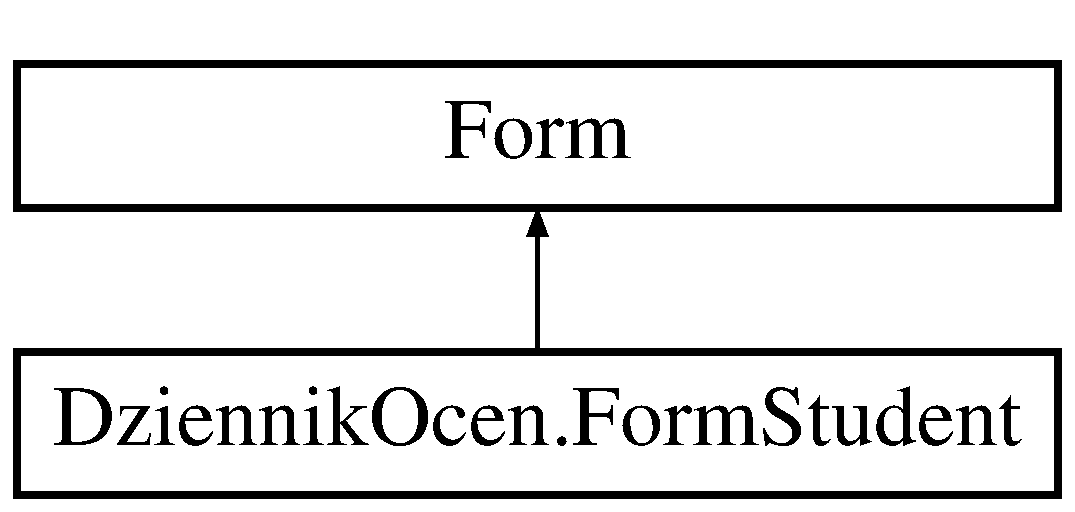
\includegraphics[height=2.000000cm]{class_dziennik_ocen_1_1_form_student}
\end{center}
\end{figure}
\subsection*{Public Member Functions}
\begin{DoxyCompactItemize}
\item 
\hyperlink{class_dziennik_ocen_1_1_form_student_a180a91bbe1f167c994a1ac4c6464c495}{Form\+Student} (string \hyperlink{class_dziennik_ocen_1_1_form_student_a99d078499cfc9792c35a2e24bc379eaa}{Email}, string \hyperlink{class_dziennik_ocen_1_1_form_student_a605a1d835840f2800e5f86171d6dbe07}{Haslo})
\item 
\hyperlink{class_dziennik_ocen_1_1_s_t_u_d_e_n_t}{S\+T\+U\+D\+E\+NT} \hyperlink{class_dziennik_ocen_1_1_form_student_a2e4d1c0eee057f3843c967d3d3cb0be4}{Znajdz\+Studenta} (string \hyperlink{class_dziennik_ocen_1_1_form_student_a99d078499cfc9792c35a2e24bc379eaa}{Email}, string \hyperlink{class_dziennik_ocen_1_1_form_student_a605a1d835840f2800e5f86171d6dbe07}{Haslo})
\item 
\hyperlink{class_dziennik_ocen_1_1_p_r_o_j_e_k_t}{P\+R\+O\+J\+E\+KT} \hyperlink{class_dziennik_ocen_1_1_form_student_a14d788ebef23a75272beea8760885a0a}{Znajdz\+Projekt} (string nazwa)
\item 
\hyperlink{class_dziennik_ocen_1_1_p_r_o_w_a_d_z_xC4_x84_c_y}{P\+R\+O\+W\+A\+D\+ZĄ\+CY} \hyperlink{class_dziennik_ocen_1_1_form_student_ab07c634bad05aec5c88b1eb7a221dd88}{Znajdz\+Prowadzacego} (string \hyperlink{class_dziennik_ocen_1_1_form_student_a9809e038a5e376197dd5fbb861fd0740}{nazwa\+\_\+przedmiotu})
\end{DoxyCompactItemize}
\subsection*{Protected Member Functions}
\begin{DoxyCompactItemize}
\item 
override void \hyperlink{class_dziennik_ocen_1_1_form_student_a2b1c3e297618729ddc9b97963d9bddda}{Dispose} (bool disposing)
\begin{DoxyCompactList}\small\item\em Clean up any resources being used. \end{DoxyCompactList}\end{DoxyCompactItemize}
\subsection*{Private Member Functions}
\begin{DoxyCompactItemize}
\item 
void \hyperlink{class_dziennik_ocen_1_1_form_student_a610e562e883311501715fb9066284c98}{Zaladuj\+Przedmioty} ()
\item 
void \hyperlink{class_dziennik_ocen_1_1_form_student_a533c3fec9f9f828b13c367ec9f3704b4}{Zaladuj\+Dane\+Studenta} ()
\item 
void \hyperlink{class_dziennik_ocen_1_1_form_student_adde6792fcf3f864c856ccd7bca293add}{Zaladuj\+Projekty} ()
\item 
void \hyperlink{class_dziennik_ocen_1_1_form_student_af8be97cad78cc0a85ea9528f5e8cc312}{Zaladuj\+Moje\+Projekty} ()
\item 
void \hyperlink{class_dziennik_ocen_1_1_form_student_a867ea1d076f7fd4dc7bfa6f3b870b52d}{przedmioty\+Tool\+Strip\+Menu\+Item\+\_\+\+Click} (object sender, Event\+Args e)
\item 
void \hyperlink{class_dziennik_ocen_1_1_form_student_aeec318394ab1b1e00a8f0d6ab5d15e3a}{student\+Tool\+Strip\+Menu\+Item\+\_\+\+Click} (object sender, Event\+Args e)
\item 
void \hyperlink{class_dziennik_ocen_1_1_form_student_af5850ddba074f1119817ad279db6b326}{projekty\+Tool\+Strip\+Menu\+Item\+\_\+\+Click} (object sender, Event\+Args e)
\item 
void \hyperlink{class_dziennik_ocen_1_1_form_student_a7c84c02d2fb4636dece7caf2c88a4d13}{dgv\+Projekty\+\_\+\+Selection\+Changed} (object sender, Event\+Args e)
\item 
void \hyperlink{class_dziennik_ocen_1_1_form_student_ae74000b681a9c5958ab1369820a6bf4c}{button1\+\_\+\+Click} (object sender, Event\+Args e)
\item 
void \hyperlink{class_dziennik_ocen_1_1_form_student_af42ad894b5a65d57d81bcf90ac1568dd}{Form\+Student\+\_\+\+Form\+Closing} (object sender, Form\+Closing\+Event\+Args e)
\item 
void \hyperlink{class_dziennik_ocen_1_1_form_student_a52bcdd2774ac5ad7145ad5602d923ad1}{Initialize\+Component} ()
\begin{DoxyCompactList}\small\item\em Required method for Designer support -\/ do not modify the contents of this method with the code editor. \end{DoxyCompactList}\end{DoxyCompactItemize}
\subsection*{Private Attributes}
\begin{DoxyCompactItemize}
\item 
\hyperlink{class_dziennik_ocen_1_1_s_t_u_d_e_n_t}{S\+T\+U\+D\+E\+NT} \hyperlink{class_dziennik_ocen_1_1_form_student_aaaed39105e65a3377268c2fcec6210f1}{student}
\item 
\hyperlink{class_dziennik_ocen_1_1_dziennik_ocen_entities}{Dziennik\+Ocen\+Entities} \hyperlink{class_dziennik_ocen_1_1_form_student_a3a9019b975016197789c3c90ec0efdef}{db} = new \hyperlink{class_dziennik_ocen_1_1_dziennik_ocen_entities}{Dziennik\+Ocen\+Entities}()
\item 
String \hyperlink{class_dziennik_ocen_1_1_form_student_a605a1d835840f2800e5f86171d6dbe07}{Haslo}
\item 
String \hyperlink{class_dziennik_ocen_1_1_form_student_a99d078499cfc9792c35a2e24bc379eaa}{Email}
\item 
\hyperlink{class_dziennik_ocen_1_1projekty}{projekty} \hyperlink{class_dziennik_ocen_1_1_form_student_a19d7a045f784efdea81c63cba2b7790e}{projekty}
\item 
\hyperlink{class_dziennik_ocen_1_1_p_r_o_j_e_k_t}{P\+R\+O\+J\+E\+KT} \hyperlink{class_dziennik_ocen_1_1_form_student_a07f299e38f5101c74ccc1457a8ad5140}{projekt}
\item 
\hyperlink{class_dziennik_ocen_1_1_p_r_o_w_a_d_z_xC4_x84_c_y}{P\+R\+O\+W\+A\+D\+ZĄ\+CY} \hyperlink{class_dziennik_ocen_1_1_form_student_a0c2713944091a51472ddee03e6bbf89f}{prowadzacy}
\item 
String \hyperlink{class_dziennik_ocen_1_1_form_student_adc736f606ec04500d5aa4d863f5bf5f7}{String\+\_\+nazwa\+\_\+projektu}
\item 
String \hyperlink{class_dziennik_ocen_1_1_form_student_a2702dfb84796524735a0ffe6d818fb85}{String\+\_\+nazwa\+\_\+przedmiotu}
\item 
System.\+Component\+Model.\+I\+Container \hyperlink{class_dziennik_ocen_1_1_form_student_a51980b83afbb6d6e6a8204c853243527}{components} = null
\begin{DoxyCompactList}\small\item\em Required designer variable. \end{DoxyCompactList}\item 
System.\+Windows.\+Forms.\+Menu\+Strip \hyperlink{class_dziennik_ocen_1_1_form_student_aad32af9f2db63885de87e9d52531b3ed}{menu\+Strip1}
\item 
System.\+Windows.\+Forms.\+Tool\+Strip\+Menu\+Item \hyperlink{class_dziennik_ocen_1_1_form_student_ab9ae6e2b2b722f8d4b90c1988b68f04a}{przedmioty\+Tool\+Strip\+Menu\+Item}
\item 
System.\+Windows.\+Forms.\+Tool\+Strip\+Menu\+Item \hyperlink{class_dziennik_ocen_1_1_form_student_a81c962610d454907184a68ead246043a}{student\+Tool\+Strip\+Menu\+Item}
\item 
System.\+Windows.\+Forms.\+Tool\+Strip\+Menu\+Item \hyperlink{class_dziennik_ocen_1_1_form_student_abe4d99d118caf2dd3a83520c7c8959a5}{projekty\+Tool\+Strip\+Menu\+Item}
\item 
System.\+Windows.\+Forms.\+Data\+Grid\+View \hyperlink{class_dziennik_ocen_1_1_form_student_add708c323708298fe045443191d3e460}{dgv\+Przedmioty}
\item 
System.\+Windows.\+Forms.\+Binding\+Source \hyperlink{class_dziennik_ocen_1_1_form_student_ab7aa9f85423ddc31529463cd1090aea4}{bs\+Przedmioty}
\item 
System.\+Windows.\+Forms.\+Binding\+Source \hyperlink{class_dziennik_ocen_1_1_form_student_a11ca8056f8886a9901f8b2faf61752ac}{bs\+Przedmiot}
\item 
System.\+Windows.\+Forms.\+Data\+Grid\+View\+Text\+Box\+Column \hyperlink{class_dziennik_ocen_1_1_form_student_a9809e038a5e376197dd5fbb861fd0740}{nazwa\+\_\+przedmiotu}
\item 
System.\+Windows.\+Forms.\+Data\+Grid\+View\+Text\+Box\+Column \hyperlink{class_dziennik_ocen_1_1_form_student_a60bcd7a58082934557af5075cbd7ccfa}{imie\+\_\+prowadzacego}
\item 
System.\+Windows.\+Forms.\+Data\+Grid\+View\+Text\+Box\+Column \hyperlink{class_dziennik_ocen_1_1_form_student_a8e07d405ca0f4b4f5f7523532412c542}{nazwisko\+\_\+prowadzacego}
\item 
System.\+Windows.\+Forms.\+Data\+Grid\+View\+Text\+Box\+Column \hyperlink{class_dziennik_ocen_1_1_form_student_a59ad819ffe8a8bc989fbe2ffd30d00ce}{ocena\+\_\+przedmiotu}
\item 
System.\+Windows.\+Forms.\+Data\+Grid\+View\+Text\+Box\+Column \hyperlink{class_dziennik_ocen_1_1_form_student_acfb521b7766430c6b5cbe1caa2fa1a14}{datazaliczeniaprzedmiotu\+Data\+Grid\+View\+Text\+Box\+Column}
\item 
System.\+Windows.\+Forms.\+Data\+Grid\+View\+Text\+Box\+Column \hyperlink{class_dziennik_ocen_1_1_form_student_a74dad6dadfd0510d449ca61b08ca26dc}{E\+C\+TS}
\item 
System.\+Windows.\+Forms.\+Data\+Grid\+View\+Text\+Box\+Column \hyperlink{class_dziennik_ocen_1_1_form_student_a920b3854d830dc870dba5765710fc28d}{uwagiprzedmiotu\+Data\+Grid\+View\+Text\+Box\+Column}
\item 
System.\+Windows.\+Forms.\+Data\+Grid\+View \hyperlink{class_dziennik_ocen_1_1_form_student_a375564d2938cbebbdb9ec4ca4e20ee1c}{dgv\+Student}
\item 
System.\+Windows.\+Forms.\+Binding\+Source \hyperlink{class_dziennik_ocen_1_1_form_student_a70c4ab0ecfb4aa90923562f2296a29bf}{bs\+Student}
\item 
System.\+Windows.\+Forms.\+Data\+Grid\+View\+Text\+Box\+Column \hyperlink{class_dziennik_ocen_1_1_form_student_a77df75fb06fa5e0c5d28109a0fdf017b}{id\+G\+R\+U\+P\+Y\+Data\+Grid\+View\+Text\+Box\+Column}
\item 
System.\+Windows.\+Forms.\+Data\+Grid\+View\+Text\+Box\+Column \hyperlink{class_dziennik_ocen_1_1_form_student_aeab178cb64c3f5a9232d052c03115420}{imie\+Data\+Grid\+View\+Text\+Box\+Column}
\item 
System.\+Windows.\+Forms.\+Data\+Grid\+View\+Text\+Box\+Column \hyperlink{class_dziennik_ocen_1_1_form_student_a017b724e3d91906b75adf31e5e05f9ee}{nazwisko\+Data\+Grid\+View\+Text\+Box\+Column}
\item 
System.\+Windows.\+Forms.\+Data\+Grid\+View\+Text\+Box\+Column \hyperlink{class_dziennik_ocen_1_1_form_student_a77809a3c1211ddf397d615357ebf9982}{telefon\+Data\+Grid\+View\+Text\+Box\+Column}
\item 
System.\+Windows.\+Forms.\+Data\+Grid\+View\+Text\+Box\+Column \hyperlink{class_dziennik_ocen_1_1_form_student_a9670f026137e2799df4901138ea44fe0}{adres\+Data\+Grid\+View\+Text\+Box\+Column}
\item 
System.\+Windows.\+Forms.\+Data\+Grid\+View\+Text\+Box\+Column \hyperlink{class_dziennik_ocen_1_1_form_student_a938dabf12cf4dbf3c3821356271b6c90}{email\+Data\+Grid\+View\+Text\+Box\+Column}
\item 
System.\+Windows.\+Forms.\+Data\+Grid\+View\+Text\+Box\+Column \hyperlink{class_dziennik_ocen_1_1_form_student_aa3a09279916f9f9af11df4ca4f4e4a2a}{haslo\+Data\+Grid\+View\+Text\+Box\+Column}
\item 
System.\+Windows.\+Forms.\+Data\+Grid\+View \hyperlink{class_dziennik_ocen_1_1_form_student_a7d9abb2899119208b489ed60f26f12e5}{dgv\+Projekty}
\item 
System.\+Windows.\+Forms.\+Data\+Grid\+View \hyperlink{class_dziennik_ocen_1_1_form_student_a0228009ac4ed48fc4ad1bee184883b84}{dgv\+Moje\+Projekty}
\item 
System.\+Windows.\+Forms.\+Binding\+Source \hyperlink{class_dziennik_ocen_1_1_form_student_af848e4daa2793882a2b76cd164fde330}{bs\+Projekty}
\item 
System.\+Windows.\+Forms.\+Button \hyperlink{class_dziennik_ocen_1_1_form_student_a257a59fdf1636c5a6741c42db75714df}{button1}
\end{DoxyCompactItemize}


\subsection{Constructor \& Destructor Documentation}
\mbox{\Hypertarget{class_dziennik_ocen_1_1_form_student_a180a91bbe1f167c994a1ac4c6464c495}\label{class_dziennik_ocen_1_1_form_student_a180a91bbe1f167c994a1ac4c6464c495}} 
\index{Dziennik\+Ocen\+::\+Form\+Student@{Dziennik\+Ocen\+::\+Form\+Student}!Form\+Student@{Form\+Student}}
\index{Form\+Student@{Form\+Student}!Dziennik\+Ocen\+::\+Form\+Student@{Dziennik\+Ocen\+::\+Form\+Student}}
\subsubsection{\texorpdfstring{Form\+Student()}{FormStudent()}}
{\footnotesize\ttfamily Dziennik\+Ocen.\+Form\+Student.\+Form\+Student (\begin{DoxyParamCaption}\item[{string}]{Email,  }\item[{string}]{Haslo }\end{DoxyParamCaption})\hspace{0.3cm}{\ttfamily [inline]}}



\subsection{Member Function Documentation}
\mbox{\Hypertarget{class_dziennik_ocen_1_1_form_student_ae74000b681a9c5958ab1369820a6bf4c}\label{class_dziennik_ocen_1_1_form_student_ae74000b681a9c5958ab1369820a6bf4c}} 
\index{Dziennik\+Ocen\+::\+Form\+Student@{Dziennik\+Ocen\+::\+Form\+Student}!button1\+\_\+\+Click@{button1\+\_\+\+Click}}
\index{button1\+\_\+\+Click@{button1\+\_\+\+Click}!Dziennik\+Ocen\+::\+Form\+Student@{Dziennik\+Ocen\+::\+Form\+Student}}
\subsubsection{\texorpdfstring{button1\+\_\+\+Click()}{button1\_Click()}}
{\footnotesize\ttfamily void Dziennik\+Ocen.\+Form\+Student.\+button1\+\_\+\+Click (\begin{DoxyParamCaption}\item[{object}]{sender,  }\item[{Event\+Args}]{e }\end{DoxyParamCaption})\hspace{0.3cm}{\ttfamily [inline]}, {\ttfamily [private]}}

\mbox{\Hypertarget{class_dziennik_ocen_1_1_form_student_a7c84c02d2fb4636dece7caf2c88a4d13}\label{class_dziennik_ocen_1_1_form_student_a7c84c02d2fb4636dece7caf2c88a4d13}} 
\index{Dziennik\+Ocen\+::\+Form\+Student@{Dziennik\+Ocen\+::\+Form\+Student}!dgv\+Projekty\+\_\+\+Selection\+Changed@{dgv\+Projekty\+\_\+\+Selection\+Changed}}
\index{dgv\+Projekty\+\_\+\+Selection\+Changed@{dgv\+Projekty\+\_\+\+Selection\+Changed}!Dziennik\+Ocen\+::\+Form\+Student@{Dziennik\+Ocen\+::\+Form\+Student}}
\subsubsection{\texorpdfstring{dgv\+Projekty\+\_\+\+Selection\+Changed()}{dgvProjekty\_SelectionChanged()}}
{\footnotesize\ttfamily void Dziennik\+Ocen.\+Form\+Student.\+dgv\+Projekty\+\_\+\+Selection\+Changed (\begin{DoxyParamCaption}\item[{object}]{sender,  }\item[{Event\+Args}]{e }\end{DoxyParamCaption})\hspace{0.3cm}{\ttfamily [inline]}, {\ttfamily [private]}}

\mbox{\Hypertarget{class_dziennik_ocen_1_1_form_student_a2b1c3e297618729ddc9b97963d9bddda}\label{class_dziennik_ocen_1_1_form_student_a2b1c3e297618729ddc9b97963d9bddda}} 
\index{Dziennik\+Ocen\+::\+Form\+Student@{Dziennik\+Ocen\+::\+Form\+Student}!Dispose@{Dispose}}
\index{Dispose@{Dispose}!Dziennik\+Ocen\+::\+Form\+Student@{Dziennik\+Ocen\+::\+Form\+Student}}
\subsubsection{\texorpdfstring{Dispose()}{Dispose()}}
{\footnotesize\ttfamily override void Dziennik\+Ocen.\+Form\+Student.\+Dispose (\begin{DoxyParamCaption}\item[{bool}]{disposing }\end{DoxyParamCaption})\hspace{0.3cm}{\ttfamily [inline]}, {\ttfamily [protected]}}



Clean up any resources being used. 


\begin{DoxyParams}{Parameters}
{\em disposing} & true if managed resources should be disposed; otherwise, false.\\
\hline
\end{DoxyParams}
\mbox{\Hypertarget{class_dziennik_ocen_1_1_form_student_af42ad894b5a65d57d81bcf90ac1568dd}\label{class_dziennik_ocen_1_1_form_student_af42ad894b5a65d57d81bcf90ac1568dd}} 
\index{Dziennik\+Ocen\+::\+Form\+Student@{Dziennik\+Ocen\+::\+Form\+Student}!Form\+Student\+\_\+\+Form\+Closing@{Form\+Student\+\_\+\+Form\+Closing}}
\index{Form\+Student\+\_\+\+Form\+Closing@{Form\+Student\+\_\+\+Form\+Closing}!Dziennik\+Ocen\+::\+Form\+Student@{Dziennik\+Ocen\+::\+Form\+Student}}
\subsubsection{\texorpdfstring{Form\+Student\+\_\+\+Form\+Closing()}{FormStudent\_FormClosing()}}
{\footnotesize\ttfamily void Dziennik\+Ocen.\+Form\+Student.\+Form\+Student\+\_\+\+Form\+Closing (\begin{DoxyParamCaption}\item[{object}]{sender,  }\item[{Form\+Closing\+Event\+Args}]{e }\end{DoxyParamCaption})\hspace{0.3cm}{\ttfamily [inline]}, {\ttfamily [private]}}

\mbox{\Hypertarget{class_dziennik_ocen_1_1_form_student_a52bcdd2774ac5ad7145ad5602d923ad1}\label{class_dziennik_ocen_1_1_form_student_a52bcdd2774ac5ad7145ad5602d923ad1}} 
\index{Dziennik\+Ocen\+::\+Form\+Student@{Dziennik\+Ocen\+::\+Form\+Student}!Initialize\+Component@{Initialize\+Component}}
\index{Initialize\+Component@{Initialize\+Component}!Dziennik\+Ocen\+::\+Form\+Student@{Dziennik\+Ocen\+::\+Form\+Student}}
\subsubsection{\texorpdfstring{Initialize\+Component()}{InitializeComponent()}}
{\footnotesize\ttfamily void Dziennik\+Ocen.\+Form\+Student.\+Initialize\+Component (\begin{DoxyParamCaption}{ }\end{DoxyParamCaption})\hspace{0.3cm}{\ttfamily [inline]}, {\ttfamily [private]}}



Required method for Designer support -\/ do not modify the contents of this method with the code editor. 

\mbox{\Hypertarget{class_dziennik_ocen_1_1_form_student_af5850ddba074f1119817ad279db6b326}\label{class_dziennik_ocen_1_1_form_student_af5850ddba074f1119817ad279db6b326}} 
\index{Dziennik\+Ocen\+::\+Form\+Student@{Dziennik\+Ocen\+::\+Form\+Student}!projekty\+Tool\+Strip\+Menu\+Item\+\_\+\+Click@{projekty\+Tool\+Strip\+Menu\+Item\+\_\+\+Click}}
\index{projekty\+Tool\+Strip\+Menu\+Item\+\_\+\+Click@{projekty\+Tool\+Strip\+Menu\+Item\+\_\+\+Click}!Dziennik\+Ocen\+::\+Form\+Student@{Dziennik\+Ocen\+::\+Form\+Student}}
\subsubsection{\texorpdfstring{projekty\+Tool\+Strip\+Menu\+Item\+\_\+\+Click()}{projektyToolStripMenuItem\_Click()}}
{\footnotesize\ttfamily void Dziennik\+Ocen.\+Form\+Student.\+projekty\+Tool\+Strip\+Menu\+Item\+\_\+\+Click (\begin{DoxyParamCaption}\item[{object}]{sender,  }\item[{Event\+Args}]{e }\end{DoxyParamCaption})\hspace{0.3cm}{\ttfamily [inline]}, {\ttfamily [private]}}

\mbox{\Hypertarget{class_dziennik_ocen_1_1_form_student_a867ea1d076f7fd4dc7bfa6f3b870b52d}\label{class_dziennik_ocen_1_1_form_student_a867ea1d076f7fd4dc7bfa6f3b870b52d}} 
\index{Dziennik\+Ocen\+::\+Form\+Student@{Dziennik\+Ocen\+::\+Form\+Student}!przedmioty\+Tool\+Strip\+Menu\+Item\+\_\+\+Click@{przedmioty\+Tool\+Strip\+Menu\+Item\+\_\+\+Click}}
\index{przedmioty\+Tool\+Strip\+Menu\+Item\+\_\+\+Click@{przedmioty\+Tool\+Strip\+Menu\+Item\+\_\+\+Click}!Dziennik\+Ocen\+::\+Form\+Student@{Dziennik\+Ocen\+::\+Form\+Student}}
\subsubsection{\texorpdfstring{przedmioty\+Tool\+Strip\+Menu\+Item\+\_\+\+Click()}{przedmiotyToolStripMenuItem\_Click()}}
{\footnotesize\ttfamily void Dziennik\+Ocen.\+Form\+Student.\+przedmioty\+Tool\+Strip\+Menu\+Item\+\_\+\+Click (\begin{DoxyParamCaption}\item[{object}]{sender,  }\item[{Event\+Args}]{e }\end{DoxyParamCaption})\hspace{0.3cm}{\ttfamily [inline]}, {\ttfamily [private]}}

\mbox{\Hypertarget{class_dziennik_ocen_1_1_form_student_aeec318394ab1b1e00a8f0d6ab5d15e3a}\label{class_dziennik_ocen_1_1_form_student_aeec318394ab1b1e00a8f0d6ab5d15e3a}} 
\index{Dziennik\+Ocen\+::\+Form\+Student@{Dziennik\+Ocen\+::\+Form\+Student}!student\+Tool\+Strip\+Menu\+Item\+\_\+\+Click@{student\+Tool\+Strip\+Menu\+Item\+\_\+\+Click}}
\index{student\+Tool\+Strip\+Menu\+Item\+\_\+\+Click@{student\+Tool\+Strip\+Menu\+Item\+\_\+\+Click}!Dziennik\+Ocen\+::\+Form\+Student@{Dziennik\+Ocen\+::\+Form\+Student}}
\subsubsection{\texorpdfstring{student\+Tool\+Strip\+Menu\+Item\+\_\+\+Click()}{studentToolStripMenuItem\_Click()}}
{\footnotesize\ttfamily void Dziennik\+Ocen.\+Form\+Student.\+student\+Tool\+Strip\+Menu\+Item\+\_\+\+Click (\begin{DoxyParamCaption}\item[{object}]{sender,  }\item[{Event\+Args}]{e }\end{DoxyParamCaption})\hspace{0.3cm}{\ttfamily [inline]}, {\ttfamily [private]}}

\mbox{\Hypertarget{class_dziennik_ocen_1_1_form_student_a533c3fec9f9f828b13c367ec9f3704b4}\label{class_dziennik_ocen_1_1_form_student_a533c3fec9f9f828b13c367ec9f3704b4}} 
\index{Dziennik\+Ocen\+::\+Form\+Student@{Dziennik\+Ocen\+::\+Form\+Student}!Zaladuj\+Dane\+Studenta@{Zaladuj\+Dane\+Studenta}}
\index{Zaladuj\+Dane\+Studenta@{Zaladuj\+Dane\+Studenta}!Dziennik\+Ocen\+::\+Form\+Student@{Dziennik\+Ocen\+::\+Form\+Student}}
\subsubsection{\texorpdfstring{Zaladuj\+Dane\+Studenta()}{ZaladujDaneStudenta()}}
{\footnotesize\ttfamily void Dziennik\+Ocen.\+Form\+Student.\+Zaladuj\+Dane\+Studenta (\begin{DoxyParamCaption}{ }\end{DoxyParamCaption})\hspace{0.3cm}{\ttfamily [inline]}, {\ttfamily [private]}}

\mbox{\Hypertarget{class_dziennik_ocen_1_1_form_student_af8be97cad78cc0a85ea9528f5e8cc312}\label{class_dziennik_ocen_1_1_form_student_af8be97cad78cc0a85ea9528f5e8cc312}} 
\index{Dziennik\+Ocen\+::\+Form\+Student@{Dziennik\+Ocen\+::\+Form\+Student}!Zaladuj\+Moje\+Projekty@{Zaladuj\+Moje\+Projekty}}
\index{Zaladuj\+Moje\+Projekty@{Zaladuj\+Moje\+Projekty}!Dziennik\+Ocen\+::\+Form\+Student@{Dziennik\+Ocen\+::\+Form\+Student}}
\subsubsection{\texorpdfstring{Zaladuj\+Moje\+Projekty()}{ZaladujMojeProjekty()}}
{\footnotesize\ttfamily void Dziennik\+Ocen.\+Form\+Student.\+Zaladuj\+Moje\+Projekty (\begin{DoxyParamCaption}{ }\end{DoxyParamCaption})\hspace{0.3cm}{\ttfamily [inline]}, {\ttfamily [private]}}

\mbox{\Hypertarget{class_dziennik_ocen_1_1_form_student_adde6792fcf3f864c856ccd7bca293add}\label{class_dziennik_ocen_1_1_form_student_adde6792fcf3f864c856ccd7bca293add}} 
\index{Dziennik\+Ocen\+::\+Form\+Student@{Dziennik\+Ocen\+::\+Form\+Student}!Zaladuj\+Projekty@{Zaladuj\+Projekty}}
\index{Zaladuj\+Projekty@{Zaladuj\+Projekty}!Dziennik\+Ocen\+::\+Form\+Student@{Dziennik\+Ocen\+::\+Form\+Student}}
\subsubsection{\texorpdfstring{Zaladuj\+Projekty()}{ZaladujProjekty()}}
{\footnotesize\ttfamily void Dziennik\+Ocen.\+Form\+Student.\+Zaladuj\+Projekty (\begin{DoxyParamCaption}{ }\end{DoxyParamCaption})\hspace{0.3cm}{\ttfamily [inline]}, {\ttfamily [private]}}

\mbox{\Hypertarget{class_dziennik_ocen_1_1_form_student_a610e562e883311501715fb9066284c98}\label{class_dziennik_ocen_1_1_form_student_a610e562e883311501715fb9066284c98}} 
\index{Dziennik\+Ocen\+::\+Form\+Student@{Dziennik\+Ocen\+::\+Form\+Student}!Zaladuj\+Przedmioty@{Zaladuj\+Przedmioty}}
\index{Zaladuj\+Przedmioty@{Zaladuj\+Przedmioty}!Dziennik\+Ocen\+::\+Form\+Student@{Dziennik\+Ocen\+::\+Form\+Student}}
\subsubsection{\texorpdfstring{Zaladuj\+Przedmioty()}{ZaladujPrzedmioty()}}
{\footnotesize\ttfamily void Dziennik\+Ocen.\+Form\+Student.\+Zaladuj\+Przedmioty (\begin{DoxyParamCaption}{ }\end{DoxyParamCaption})\hspace{0.3cm}{\ttfamily [inline]}, {\ttfamily [private]}}

\mbox{\Hypertarget{class_dziennik_ocen_1_1_form_student_a14d788ebef23a75272beea8760885a0a}\label{class_dziennik_ocen_1_1_form_student_a14d788ebef23a75272beea8760885a0a}} 
\index{Dziennik\+Ocen\+::\+Form\+Student@{Dziennik\+Ocen\+::\+Form\+Student}!Znajdz\+Projekt@{Znajdz\+Projekt}}
\index{Znajdz\+Projekt@{Znajdz\+Projekt}!Dziennik\+Ocen\+::\+Form\+Student@{Dziennik\+Ocen\+::\+Form\+Student}}
\subsubsection{\texorpdfstring{Znajdz\+Projekt()}{ZnajdzProjekt()}}
{\footnotesize\ttfamily \hyperlink{class_dziennik_ocen_1_1_p_r_o_j_e_k_t}{P\+R\+O\+J\+E\+KT} Dziennik\+Ocen.\+Form\+Student.\+Znajdz\+Projekt (\begin{DoxyParamCaption}\item[{string}]{nazwa }\end{DoxyParamCaption})\hspace{0.3cm}{\ttfamily [inline]}}

\mbox{\Hypertarget{class_dziennik_ocen_1_1_form_student_ab07c634bad05aec5c88b1eb7a221dd88}\label{class_dziennik_ocen_1_1_form_student_ab07c634bad05aec5c88b1eb7a221dd88}} 
\index{Dziennik\+Ocen\+::\+Form\+Student@{Dziennik\+Ocen\+::\+Form\+Student}!Znajdz\+Prowadzacego@{Znajdz\+Prowadzacego}}
\index{Znajdz\+Prowadzacego@{Znajdz\+Prowadzacego}!Dziennik\+Ocen\+::\+Form\+Student@{Dziennik\+Ocen\+::\+Form\+Student}}
\subsubsection{\texorpdfstring{Znajdz\+Prowadzacego()}{ZnajdzProwadzacego()}}
{\footnotesize\ttfamily \hyperlink{class_dziennik_ocen_1_1_p_r_o_w_a_d_z_xC4_x84_c_y}{P\+R\+O\+W\+A\+D\+ZĄ\+CY} Dziennik\+Ocen.\+Form\+Student.\+Znajdz\+Prowadzacego (\begin{DoxyParamCaption}\item[{string}]{nazwa\+\_\+przedmiotu }\end{DoxyParamCaption})\hspace{0.3cm}{\ttfamily [inline]}}

\mbox{\Hypertarget{class_dziennik_ocen_1_1_form_student_a2e4d1c0eee057f3843c967d3d3cb0be4}\label{class_dziennik_ocen_1_1_form_student_a2e4d1c0eee057f3843c967d3d3cb0be4}} 
\index{Dziennik\+Ocen\+::\+Form\+Student@{Dziennik\+Ocen\+::\+Form\+Student}!Znajdz\+Studenta@{Znajdz\+Studenta}}
\index{Znajdz\+Studenta@{Znajdz\+Studenta}!Dziennik\+Ocen\+::\+Form\+Student@{Dziennik\+Ocen\+::\+Form\+Student}}
\subsubsection{\texorpdfstring{Znajdz\+Studenta()}{ZnajdzStudenta()}}
{\footnotesize\ttfamily \hyperlink{class_dziennik_ocen_1_1_s_t_u_d_e_n_t}{S\+T\+U\+D\+E\+NT} Dziennik\+Ocen.\+Form\+Student.\+Znajdz\+Studenta (\begin{DoxyParamCaption}\item[{string}]{Email,  }\item[{string}]{Haslo }\end{DoxyParamCaption})\hspace{0.3cm}{\ttfamily [inline]}}



\subsection{Member Data Documentation}
\mbox{\Hypertarget{class_dziennik_ocen_1_1_form_student_a9670f026137e2799df4901138ea44fe0}\label{class_dziennik_ocen_1_1_form_student_a9670f026137e2799df4901138ea44fe0}} 
\index{Dziennik\+Ocen\+::\+Form\+Student@{Dziennik\+Ocen\+::\+Form\+Student}!adres\+Data\+Grid\+View\+Text\+Box\+Column@{adres\+Data\+Grid\+View\+Text\+Box\+Column}}
\index{adres\+Data\+Grid\+View\+Text\+Box\+Column@{adres\+Data\+Grid\+View\+Text\+Box\+Column}!Dziennik\+Ocen\+::\+Form\+Student@{Dziennik\+Ocen\+::\+Form\+Student}}
\subsubsection{\texorpdfstring{adres\+Data\+Grid\+View\+Text\+Box\+Column}{adresDataGridViewTextBoxColumn}}
{\footnotesize\ttfamily System.\+Windows.\+Forms.\+Data\+Grid\+View\+Text\+Box\+Column Dziennik\+Ocen.\+Form\+Student.\+adres\+Data\+Grid\+View\+Text\+Box\+Column\hspace{0.3cm}{\ttfamily [private]}}

\mbox{\Hypertarget{class_dziennik_ocen_1_1_form_student_af848e4daa2793882a2b76cd164fde330}\label{class_dziennik_ocen_1_1_form_student_af848e4daa2793882a2b76cd164fde330}} 
\index{Dziennik\+Ocen\+::\+Form\+Student@{Dziennik\+Ocen\+::\+Form\+Student}!bs\+Projekty@{bs\+Projekty}}
\index{bs\+Projekty@{bs\+Projekty}!Dziennik\+Ocen\+::\+Form\+Student@{Dziennik\+Ocen\+::\+Form\+Student}}
\subsubsection{\texorpdfstring{bs\+Projekty}{bsProjekty}}
{\footnotesize\ttfamily System.\+Windows.\+Forms.\+Binding\+Source Dziennik\+Ocen.\+Form\+Student.\+bs\+Projekty\hspace{0.3cm}{\ttfamily [private]}}

\mbox{\Hypertarget{class_dziennik_ocen_1_1_form_student_a11ca8056f8886a9901f8b2faf61752ac}\label{class_dziennik_ocen_1_1_form_student_a11ca8056f8886a9901f8b2faf61752ac}} 
\index{Dziennik\+Ocen\+::\+Form\+Student@{Dziennik\+Ocen\+::\+Form\+Student}!bs\+Przedmiot@{bs\+Przedmiot}}
\index{bs\+Przedmiot@{bs\+Przedmiot}!Dziennik\+Ocen\+::\+Form\+Student@{Dziennik\+Ocen\+::\+Form\+Student}}
\subsubsection{\texorpdfstring{bs\+Przedmiot}{bsPrzedmiot}}
{\footnotesize\ttfamily System.\+Windows.\+Forms.\+Binding\+Source Dziennik\+Ocen.\+Form\+Student.\+bs\+Przedmiot\hspace{0.3cm}{\ttfamily [private]}}

\mbox{\Hypertarget{class_dziennik_ocen_1_1_form_student_ab7aa9f85423ddc31529463cd1090aea4}\label{class_dziennik_ocen_1_1_form_student_ab7aa9f85423ddc31529463cd1090aea4}} 
\index{Dziennik\+Ocen\+::\+Form\+Student@{Dziennik\+Ocen\+::\+Form\+Student}!bs\+Przedmioty@{bs\+Przedmioty}}
\index{bs\+Przedmioty@{bs\+Przedmioty}!Dziennik\+Ocen\+::\+Form\+Student@{Dziennik\+Ocen\+::\+Form\+Student}}
\subsubsection{\texorpdfstring{bs\+Przedmioty}{bsPrzedmioty}}
{\footnotesize\ttfamily System.\+Windows.\+Forms.\+Binding\+Source Dziennik\+Ocen.\+Form\+Student.\+bs\+Przedmioty\hspace{0.3cm}{\ttfamily [private]}}

\mbox{\Hypertarget{class_dziennik_ocen_1_1_form_student_a70c4ab0ecfb4aa90923562f2296a29bf}\label{class_dziennik_ocen_1_1_form_student_a70c4ab0ecfb4aa90923562f2296a29bf}} 
\index{Dziennik\+Ocen\+::\+Form\+Student@{Dziennik\+Ocen\+::\+Form\+Student}!bs\+Student@{bs\+Student}}
\index{bs\+Student@{bs\+Student}!Dziennik\+Ocen\+::\+Form\+Student@{Dziennik\+Ocen\+::\+Form\+Student}}
\subsubsection{\texorpdfstring{bs\+Student}{bsStudent}}
{\footnotesize\ttfamily System.\+Windows.\+Forms.\+Binding\+Source Dziennik\+Ocen.\+Form\+Student.\+bs\+Student\hspace{0.3cm}{\ttfamily [private]}}

\mbox{\Hypertarget{class_dziennik_ocen_1_1_form_student_a257a59fdf1636c5a6741c42db75714df}\label{class_dziennik_ocen_1_1_form_student_a257a59fdf1636c5a6741c42db75714df}} 
\index{Dziennik\+Ocen\+::\+Form\+Student@{Dziennik\+Ocen\+::\+Form\+Student}!button1@{button1}}
\index{button1@{button1}!Dziennik\+Ocen\+::\+Form\+Student@{Dziennik\+Ocen\+::\+Form\+Student}}
\subsubsection{\texorpdfstring{button1}{button1}}
{\footnotesize\ttfamily System.\+Windows.\+Forms.\+Button Dziennik\+Ocen.\+Form\+Student.\+button1\hspace{0.3cm}{\ttfamily [private]}}

\mbox{\Hypertarget{class_dziennik_ocen_1_1_form_student_a51980b83afbb6d6e6a8204c853243527}\label{class_dziennik_ocen_1_1_form_student_a51980b83afbb6d6e6a8204c853243527}} 
\index{Dziennik\+Ocen\+::\+Form\+Student@{Dziennik\+Ocen\+::\+Form\+Student}!components@{components}}
\index{components@{components}!Dziennik\+Ocen\+::\+Form\+Student@{Dziennik\+Ocen\+::\+Form\+Student}}
\subsubsection{\texorpdfstring{components}{components}}
{\footnotesize\ttfamily System.\+Component\+Model.\+I\+Container Dziennik\+Ocen.\+Form\+Student.\+components = null\hspace{0.3cm}{\ttfamily [private]}}



Required designer variable. 

\mbox{\Hypertarget{class_dziennik_ocen_1_1_form_student_acfb521b7766430c6b5cbe1caa2fa1a14}\label{class_dziennik_ocen_1_1_form_student_acfb521b7766430c6b5cbe1caa2fa1a14}} 
\index{Dziennik\+Ocen\+::\+Form\+Student@{Dziennik\+Ocen\+::\+Form\+Student}!datazaliczeniaprzedmiotu\+Data\+Grid\+View\+Text\+Box\+Column@{datazaliczeniaprzedmiotu\+Data\+Grid\+View\+Text\+Box\+Column}}
\index{datazaliczeniaprzedmiotu\+Data\+Grid\+View\+Text\+Box\+Column@{datazaliczeniaprzedmiotu\+Data\+Grid\+View\+Text\+Box\+Column}!Dziennik\+Ocen\+::\+Form\+Student@{Dziennik\+Ocen\+::\+Form\+Student}}
\subsubsection{\texorpdfstring{datazaliczeniaprzedmiotu\+Data\+Grid\+View\+Text\+Box\+Column}{datazaliczeniaprzedmiotuDataGridViewTextBoxColumn}}
{\footnotesize\ttfamily System.\+Windows.\+Forms.\+Data\+Grid\+View\+Text\+Box\+Column Dziennik\+Ocen.\+Form\+Student.\+datazaliczeniaprzedmiotu\+Data\+Grid\+View\+Text\+Box\+Column\hspace{0.3cm}{\ttfamily [private]}}

\mbox{\Hypertarget{class_dziennik_ocen_1_1_form_student_a3a9019b975016197789c3c90ec0efdef}\label{class_dziennik_ocen_1_1_form_student_a3a9019b975016197789c3c90ec0efdef}} 
\index{Dziennik\+Ocen\+::\+Form\+Student@{Dziennik\+Ocen\+::\+Form\+Student}!db@{db}}
\index{db@{db}!Dziennik\+Ocen\+::\+Form\+Student@{Dziennik\+Ocen\+::\+Form\+Student}}
\subsubsection{\texorpdfstring{db}{db}}
{\footnotesize\ttfamily \hyperlink{class_dziennik_ocen_1_1_dziennik_ocen_entities}{Dziennik\+Ocen\+Entities} Dziennik\+Ocen.\+Form\+Student.\+db = new \hyperlink{class_dziennik_ocen_1_1_dziennik_ocen_entities}{Dziennik\+Ocen\+Entities}()\hspace{0.3cm}{\ttfamily [private]}}

\mbox{\Hypertarget{class_dziennik_ocen_1_1_form_student_a0228009ac4ed48fc4ad1bee184883b84}\label{class_dziennik_ocen_1_1_form_student_a0228009ac4ed48fc4ad1bee184883b84}} 
\index{Dziennik\+Ocen\+::\+Form\+Student@{Dziennik\+Ocen\+::\+Form\+Student}!dgv\+Moje\+Projekty@{dgv\+Moje\+Projekty}}
\index{dgv\+Moje\+Projekty@{dgv\+Moje\+Projekty}!Dziennik\+Ocen\+::\+Form\+Student@{Dziennik\+Ocen\+::\+Form\+Student}}
\subsubsection{\texorpdfstring{dgv\+Moje\+Projekty}{dgvMojeProjekty}}
{\footnotesize\ttfamily System.\+Windows.\+Forms.\+Data\+Grid\+View Dziennik\+Ocen.\+Form\+Student.\+dgv\+Moje\+Projekty\hspace{0.3cm}{\ttfamily [private]}}

\mbox{\Hypertarget{class_dziennik_ocen_1_1_form_student_a7d9abb2899119208b489ed60f26f12e5}\label{class_dziennik_ocen_1_1_form_student_a7d9abb2899119208b489ed60f26f12e5}} 
\index{Dziennik\+Ocen\+::\+Form\+Student@{Dziennik\+Ocen\+::\+Form\+Student}!dgv\+Projekty@{dgv\+Projekty}}
\index{dgv\+Projekty@{dgv\+Projekty}!Dziennik\+Ocen\+::\+Form\+Student@{Dziennik\+Ocen\+::\+Form\+Student}}
\subsubsection{\texorpdfstring{dgv\+Projekty}{dgvProjekty}}
{\footnotesize\ttfamily System.\+Windows.\+Forms.\+Data\+Grid\+View Dziennik\+Ocen.\+Form\+Student.\+dgv\+Projekty\hspace{0.3cm}{\ttfamily [private]}}

\mbox{\Hypertarget{class_dziennik_ocen_1_1_form_student_add708c323708298fe045443191d3e460}\label{class_dziennik_ocen_1_1_form_student_add708c323708298fe045443191d3e460}} 
\index{Dziennik\+Ocen\+::\+Form\+Student@{Dziennik\+Ocen\+::\+Form\+Student}!dgv\+Przedmioty@{dgv\+Przedmioty}}
\index{dgv\+Przedmioty@{dgv\+Przedmioty}!Dziennik\+Ocen\+::\+Form\+Student@{Dziennik\+Ocen\+::\+Form\+Student}}
\subsubsection{\texorpdfstring{dgv\+Przedmioty}{dgvPrzedmioty}}
{\footnotesize\ttfamily System.\+Windows.\+Forms.\+Data\+Grid\+View Dziennik\+Ocen.\+Form\+Student.\+dgv\+Przedmioty\hspace{0.3cm}{\ttfamily [private]}}

\mbox{\Hypertarget{class_dziennik_ocen_1_1_form_student_a375564d2938cbebbdb9ec4ca4e20ee1c}\label{class_dziennik_ocen_1_1_form_student_a375564d2938cbebbdb9ec4ca4e20ee1c}} 
\index{Dziennik\+Ocen\+::\+Form\+Student@{Dziennik\+Ocen\+::\+Form\+Student}!dgv\+Student@{dgv\+Student}}
\index{dgv\+Student@{dgv\+Student}!Dziennik\+Ocen\+::\+Form\+Student@{Dziennik\+Ocen\+::\+Form\+Student}}
\subsubsection{\texorpdfstring{dgv\+Student}{dgvStudent}}
{\footnotesize\ttfamily System.\+Windows.\+Forms.\+Data\+Grid\+View Dziennik\+Ocen.\+Form\+Student.\+dgv\+Student\hspace{0.3cm}{\ttfamily [private]}}

\mbox{\Hypertarget{class_dziennik_ocen_1_1_form_student_a74dad6dadfd0510d449ca61b08ca26dc}\label{class_dziennik_ocen_1_1_form_student_a74dad6dadfd0510d449ca61b08ca26dc}} 
\index{Dziennik\+Ocen\+::\+Form\+Student@{Dziennik\+Ocen\+::\+Form\+Student}!E\+C\+TS@{E\+C\+TS}}
\index{E\+C\+TS@{E\+C\+TS}!Dziennik\+Ocen\+::\+Form\+Student@{Dziennik\+Ocen\+::\+Form\+Student}}
\subsubsection{\texorpdfstring{E\+C\+TS}{ECTS}}
{\footnotesize\ttfamily System.\+Windows.\+Forms.\+Data\+Grid\+View\+Text\+Box\+Column Dziennik\+Ocen.\+Form\+Student.\+E\+C\+TS\hspace{0.3cm}{\ttfamily [private]}}

\mbox{\Hypertarget{class_dziennik_ocen_1_1_form_student_a99d078499cfc9792c35a2e24bc379eaa}\label{class_dziennik_ocen_1_1_form_student_a99d078499cfc9792c35a2e24bc379eaa}} 
\index{Dziennik\+Ocen\+::\+Form\+Student@{Dziennik\+Ocen\+::\+Form\+Student}!Email@{Email}}
\index{Email@{Email}!Dziennik\+Ocen\+::\+Form\+Student@{Dziennik\+Ocen\+::\+Form\+Student}}
\subsubsection{\texorpdfstring{Email}{Email}}
{\footnotesize\ttfamily String Dziennik\+Ocen.\+Form\+Student.\+Email\hspace{0.3cm}{\ttfamily [private]}}

\mbox{\Hypertarget{class_dziennik_ocen_1_1_form_student_a938dabf12cf4dbf3c3821356271b6c90}\label{class_dziennik_ocen_1_1_form_student_a938dabf12cf4dbf3c3821356271b6c90}} 
\index{Dziennik\+Ocen\+::\+Form\+Student@{Dziennik\+Ocen\+::\+Form\+Student}!email\+Data\+Grid\+View\+Text\+Box\+Column@{email\+Data\+Grid\+View\+Text\+Box\+Column}}
\index{email\+Data\+Grid\+View\+Text\+Box\+Column@{email\+Data\+Grid\+View\+Text\+Box\+Column}!Dziennik\+Ocen\+::\+Form\+Student@{Dziennik\+Ocen\+::\+Form\+Student}}
\subsubsection{\texorpdfstring{email\+Data\+Grid\+View\+Text\+Box\+Column}{emailDataGridViewTextBoxColumn}}
{\footnotesize\ttfamily System.\+Windows.\+Forms.\+Data\+Grid\+View\+Text\+Box\+Column Dziennik\+Ocen.\+Form\+Student.\+email\+Data\+Grid\+View\+Text\+Box\+Column\hspace{0.3cm}{\ttfamily [private]}}

\mbox{\Hypertarget{class_dziennik_ocen_1_1_form_student_a605a1d835840f2800e5f86171d6dbe07}\label{class_dziennik_ocen_1_1_form_student_a605a1d835840f2800e5f86171d6dbe07}} 
\index{Dziennik\+Ocen\+::\+Form\+Student@{Dziennik\+Ocen\+::\+Form\+Student}!Haslo@{Haslo}}
\index{Haslo@{Haslo}!Dziennik\+Ocen\+::\+Form\+Student@{Dziennik\+Ocen\+::\+Form\+Student}}
\subsubsection{\texorpdfstring{Haslo}{Haslo}}
{\footnotesize\ttfamily String Dziennik\+Ocen.\+Form\+Student.\+Haslo\hspace{0.3cm}{\ttfamily [private]}}

\mbox{\Hypertarget{class_dziennik_ocen_1_1_form_student_aa3a09279916f9f9af11df4ca4f4e4a2a}\label{class_dziennik_ocen_1_1_form_student_aa3a09279916f9f9af11df4ca4f4e4a2a}} 
\index{Dziennik\+Ocen\+::\+Form\+Student@{Dziennik\+Ocen\+::\+Form\+Student}!haslo\+Data\+Grid\+View\+Text\+Box\+Column@{haslo\+Data\+Grid\+View\+Text\+Box\+Column}}
\index{haslo\+Data\+Grid\+View\+Text\+Box\+Column@{haslo\+Data\+Grid\+View\+Text\+Box\+Column}!Dziennik\+Ocen\+::\+Form\+Student@{Dziennik\+Ocen\+::\+Form\+Student}}
\subsubsection{\texorpdfstring{haslo\+Data\+Grid\+View\+Text\+Box\+Column}{hasloDataGridViewTextBoxColumn}}
{\footnotesize\ttfamily System.\+Windows.\+Forms.\+Data\+Grid\+View\+Text\+Box\+Column Dziennik\+Ocen.\+Form\+Student.\+haslo\+Data\+Grid\+View\+Text\+Box\+Column\hspace{0.3cm}{\ttfamily [private]}}

\mbox{\Hypertarget{class_dziennik_ocen_1_1_form_student_a77df75fb06fa5e0c5d28109a0fdf017b}\label{class_dziennik_ocen_1_1_form_student_a77df75fb06fa5e0c5d28109a0fdf017b}} 
\index{Dziennik\+Ocen\+::\+Form\+Student@{Dziennik\+Ocen\+::\+Form\+Student}!id\+G\+R\+U\+P\+Y\+Data\+Grid\+View\+Text\+Box\+Column@{id\+G\+R\+U\+P\+Y\+Data\+Grid\+View\+Text\+Box\+Column}}
\index{id\+G\+R\+U\+P\+Y\+Data\+Grid\+View\+Text\+Box\+Column@{id\+G\+R\+U\+P\+Y\+Data\+Grid\+View\+Text\+Box\+Column}!Dziennik\+Ocen\+::\+Form\+Student@{Dziennik\+Ocen\+::\+Form\+Student}}
\subsubsection{\texorpdfstring{id\+G\+R\+U\+P\+Y\+Data\+Grid\+View\+Text\+Box\+Column}{idGRUPYDataGridViewTextBoxColumn}}
{\footnotesize\ttfamily System.\+Windows.\+Forms.\+Data\+Grid\+View\+Text\+Box\+Column Dziennik\+Ocen.\+Form\+Student.\+id\+G\+R\+U\+P\+Y\+Data\+Grid\+View\+Text\+Box\+Column\hspace{0.3cm}{\ttfamily [private]}}

\mbox{\Hypertarget{class_dziennik_ocen_1_1_form_student_a60bcd7a58082934557af5075cbd7ccfa}\label{class_dziennik_ocen_1_1_form_student_a60bcd7a58082934557af5075cbd7ccfa}} 
\index{Dziennik\+Ocen\+::\+Form\+Student@{Dziennik\+Ocen\+::\+Form\+Student}!imie\+\_\+prowadzacego@{imie\+\_\+prowadzacego}}
\index{imie\+\_\+prowadzacego@{imie\+\_\+prowadzacego}!Dziennik\+Ocen\+::\+Form\+Student@{Dziennik\+Ocen\+::\+Form\+Student}}
\subsubsection{\texorpdfstring{imie\+\_\+prowadzacego}{imie\_prowadzacego}}
{\footnotesize\ttfamily System.\+Windows.\+Forms.\+Data\+Grid\+View\+Text\+Box\+Column Dziennik\+Ocen.\+Form\+Student.\+imie\+\_\+prowadzacego\hspace{0.3cm}{\ttfamily [private]}}

\mbox{\Hypertarget{class_dziennik_ocen_1_1_form_student_aeab178cb64c3f5a9232d052c03115420}\label{class_dziennik_ocen_1_1_form_student_aeab178cb64c3f5a9232d052c03115420}} 
\index{Dziennik\+Ocen\+::\+Form\+Student@{Dziennik\+Ocen\+::\+Form\+Student}!imie\+Data\+Grid\+View\+Text\+Box\+Column@{imie\+Data\+Grid\+View\+Text\+Box\+Column}}
\index{imie\+Data\+Grid\+View\+Text\+Box\+Column@{imie\+Data\+Grid\+View\+Text\+Box\+Column}!Dziennik\+Ocen\+::\+Form\+Student@{Dziennik\+Ocen\+::\+Form\+Student}}
\subsubsection{\texorpdfstring{imie\+Data\+Grid\+View\+Text\+Box\+Column}{imieDataGridViewTextBoxColumn}}
{\footnotesize\ttfamily System.\+Windows.\+Forms.\+Data\+Grid\+View\+Text\+Box\+Column Dziennik\+Ocen.\+Form\+Student.\+imie\+Data\+Grid\+View\+Text\+Box\+Column\hspace{0.3cm}{\ttfamily [private]}}

\mbox{\Hypertarget{class_dziennik_ocen_1_1_form_student_aad32af9f2db63885de87e9d52531b3ed}\label{class_dziennik_ocen_1_1_form_student_aad32af9f2db63885de87e9d52531b3ed}} 
\index{Dziennik\+Ocen\+::\+Form\+Student@{Dziennik\+Ocen\+::\+Form\+Student}!menu\+Strip1@{menu\+Strip1}}
\index{menu\+Strip1@{menu\+Strip1}!Dziennik\+Ocen\+::\+Form\+Student@{Dziennik\+Ocen\+::\+Form\+Student}}
\subsubsection{\texorpdfstring{menu\+Strip1}{menuStrip1}}
{\footnotesize\ttfamily System.\+Windows.\+Forms.\+Menu\+Strip Dziennik\+Ocen.\+Form\+Student.\+menu\+Strip1\hspace{0.3cm}{\ttfamily [private]}}

\mbox{\Hypertarget{class_dziennik_ocen_1_1_form_student_a9809e038a5e376197dd5fbb861fd0740}\label{class_dziennik_ocen_1_1_form_student_a9809e038a5e376197dd5fbb861fd0740}} 
\index{Dziennik\+Ocen\+::\+Form\+Student@{Dziennik\+Ocen\+::\+Form\+Student}!nazwa\+\_\+przedmiotu@{nazwa\+\_\+przedmiotu}}
\index{nazwa\+\_\+przedmiotu@{nazwa\+\_\+przedmiotu}!Dziennik\+Ocen\+::\+Form\+Student@{Dziennik\+Ocen\+::\+Form\+Student}}
\subsubsection{\texorpdfstring{nazwa\+\_\+przedmiotu}{nazwa\_przedmiotu}}
{\footnotesize\ttfamily System.\+Windows.\+Forms.\+Data\+Grid\+View\+Text\+Box\+Column Dziennik\+Ocen.\+Form\+Student.\+nazwa\+\_\+przedmiotu\hspace{0.3cm}{\ttfamily [private]}}

\mbox{\Hypertarget{class_dziennik_ocen_1_1_form_student_a8e07d405ca0f4b4f5f7523532412c542}\label{class_dziennik_ocen_1_1_form_student_a8e07d405ca0f4b4f5f7523532412c542}} 
\index{Dziennik\+Ocen\+::\+Form\+Student@{Dziennik\+Ocen\+::\+Form\+Student}!nazwisko\+\_\+prowadzacego@{nazwisko\+\_\+prowadzacego}}
\index{nazwisko\+\_\+prowadzacego@{nazwisko\+\_\+prowadzacego}!Dziennik\+Ocen\+::\+Form\+Student@{Dziennik\+Ocen\+::\+Form\+Student}}
\subsubsection{\texorpdfstring{nazwisko\+\_\+prowadzacego}{nazwisko\_prowadzacego}}
{\footnotesize\ttfamily System.\+Windows.\+Forms.\+Data\+Grid\+View\+Text\+Box\+Column Dziennik\+Ocen.\+Form\+Student.\+nazwisko\+\_\+prowadzacego\hspace{0.3cm}{\ttfamily [private]}}

\mbox{\Hypertarget{class_dziennik_ocen_1_1_form_student_a017b724e3d91906b75adf31e5e05f9ee}\label{class_dziennik_ocen_1_1_form_student_a017b724e3d91906b75adf31e5e05f9ee}} 
\index{Dziennik\+Ocen\+::\+Form\+Student@{Dziennik\+Ocen\+::\+Form\+Student}!nazwisko\+Data\+Grid\+View\+Text\+Box\+Column@{nazwisko\+Data\+Grid\+View\+Text\+Box\+Column}}
\index{nazwisko\+Data\+Grid\+View\+Text\+Box\+Column@{nazwisko\+Data\+Grid\+View\+Text\+Box\+Column}!Dziennik\+Ocen\+::\+Form\+Student@{Dziennik\+Ocen\+::\+Form\+Student}}
\subsubsection{\texorpdfstring{nazwisko\+Data\+Grid\+View\+Text\+Box\+Column}{nazwiskoDataGridViewTextBoxColumn}}
{\footnotesize\ttfamily System.\+Windows.\+Forms.\+Data\+Grid\+View\+Text\+Box\+Column Dziennik\+Ocen.\+Form\+Student.\+nazwisko\+Data\+Grid\+View\+Text\+Box\+Column\hspace{0.3cm}{\ttfamily [private]}}

\mbox{\Hypertarget{class_dziennik_ocen_1_1_form_student_a59ad819ffe8a8bc989fbe2ffd30d00ce}\label{class_dziennik_ocen_1_1_form_student_a59ad819ffe8a8bc989fbe2ffd30d00ce}} 
\index{Dziennik\+Ocen\+::\+Form\+Student@{Dziennik\+Ocen\+::\+Form\+Student}!ocena\+\_\+przedmiotu@{ocena\+\_\+przedmiotu}}
\index{ocena\+\_\+przedmiotu@{ocena\+\_\+przedmiotu}!Dziennik\+Ocen\+::\+Form\+Student@{Dziennik\+Ocen\+::\+Form\+Student}}
\subsubsection{\texorpdfstring{ocena\+\_\+przedmiotu}{ocena\_przedmiotu}}
{\footnotesize\ttfamily System.\+Windows.\+Forms.\+Data\+Grid\+View\+Text\+Box\+Column Dziennik\+Ocen.\+Form\+Student.\+ocena\+\_\+przedmiotu\hspace{0.3cm}{\ttfamily [private]}}

\mbox{\Hypertarget{class_dziennik_ocen_1_1_form_student_a07f299e38f5101c74ccc1457a8ad5140}\label{class_dziennik_ocen_1_1_form_student_a07f299e38f5101c74ccc1457a8ad5140}} 
\index{Dziennik\+Ocen\+::\+Form\+Student@{Dziennik\+Ocen\+::\+Form\+Student}!projekt@{projekt}}
\index{projekt@{projekt}!Dziennik\+Ocen\+::\+Form\+Student@{Dziennik\+Ocen\+::\+Form\+Student}}
\subsubsection{\texorpdfstring{projekt}{projekt}}
{\footnotesize\ttfamily \hyperlink{class_dziennik_ocen_1_1_p_r_o_j_e_k_t}{P\+R\+O\+J\+E\+KT} Dziennik\+Ocen.\+Form\+Student.\+projekt\hspace{0.3cm}{\ttfamily [private]}}

\mbox{\Hypertarget{class_dziennik_ocen_1_1_form_student_a19d7a045f784efdea81c63cba2b7790e}\label{class_dziennik_ocen_1_1_form_student_a19d7a045f784efdea81c63cba2b7790e}} 
\index{Dziennik\+Ocen\+::\+Form\+Student@{Dziennik\+Ocen\+::\+Form\+Student}!projekty@{projekty}}
\index{projekty@{projekty}!Dziennik\+Ocen\+::\+Form\+Student@{Dziennik\+Ocen\+::\+Form\+Student}}
\subsubsection{\texorpdfstring{projekty}{projekty}}
{\footnotesize\ttfamily \hyperlink{class_dziennik_ocen_1_1projekty}{projekty} Dziennik\+Ocen.\+Form\+Student.\+projekty\hspace{0.3cm}{\ttfamily [private]}}

\mbox{\Hypertarget{class_dziennik_ocen_1_1_form_student_abe4d99d118caf2dd3a83520c7c8959a5}\label{class_dziennik_ocen_1_1_form_student_abe4d99d118caf2dd3a83520c7c8959a5}} 
\index{Dziennik\+Ocen\+::\+Form\+Student@{Dziennik\+Ocen\+::\+Form\+Student}!projekty\+Tool\+Strip\+Menu\+Item@{projekty\+Tool\+Strip\+Menu\+Item}}
\index{projekty\+Tool\+Strip\+Menu\+Item@{projekty\+Tool\+Strip\+Menu\+Item}!Dziennik\+Ocen\+::\+Form\+Student@{Dziennik\+Ocen\+::\+Form\+Student}}
\subsubsection{\texorpdfstring{projekty\+Tool\+Strip\+Menu\+Item}{projektyToolStripMenuItem}}
{\footnotesize\ttfamily System.\+Windows.\+Forms.\+Tool\+Strip\+Menu\+Item Dziennik\+Ocen.\+Form\+Student.\+projekty\+Tool\+Strip\+Menu\+Item\hspace{0.3cm}{\ttfamily [private]}}

\mbox{\Hypertarget{class_dziennik_ocen_1_1_form_student_a0c2713944091a51472ddee03e6bbf89f}\label{class_dziennik_ocen_1_1_form_student_a0c2713944091a51472ddee03e6bbf89f}} 
\index{Dziennik\+Ocen\+::\+Form\+Student@{Dziennik\+Ocen\+::\+Form\+Student}!prowadzacy@{prowadzacy}}
\index{prowadzacy@{prowadzacy}!Dziennik\+Ocen\+::\+Form\+Student@{Dziennik\+Ocen\+::\+Form\+Student}}
\subsubsection{\texorpdfstring{prowadzacy}{prowadzacy}}
{\footnotesize\ttfamily \hyperlink{class_dziennik_ocen_1_1_p_r_o_w_a_d_z_xC4_x84_c_y}{P\+R\+O\+W\+A\+D\+ZĄ\+CY} Dziennik\+Ocen.\+Form\+Student.\+prowadzacy\hspace{0.3cm}{\ttfamily [private]}}

\mbox{\Hypertarget{class_dziennik_ocen_1_1_form_student_ab9ae6e2b2b722f8d4b90c1988b68f04a}\label{class_dziennik_ocen_1_1_form_student_ab9ae6e2b2b722f8d4b90c1988b68f04a}} 
\index{Dziennik\+Ocen\+::\+Form\+Student@{Dziennik\+Ocen\+::\+Form\+Student}!przedmioty\+Tool\+Strip\+Menu\+Item@{przedmioty\+Tool\+Strip\+Menu\+Item}}
\index{przedmioty\+Tool\+Strip\+Menu\+Item@{przedmioty\+Tool\+Strip\+Menu\+Item}!Dziennik\+Ocen\+::\+Form\+Student@{Dziennik\+Ocen\+::\+Form\+Student}}
\subsubsection{\texorpdfstring{przedmioty\+Tool\+Strip\+Menu\+Item}{przedmiotyToolStripMenuItem}}
{\footnotesize\ttfamily System.\+Windows.\+Forms.\+Tool\+Strip\+Menu\+Item Dziennik\+Ocen.\+Form\+Student.\+przedmioty\+Tool\+Strip\+Menu\+Item\hspace{0.3cm}{\ttfamily [private]}}

\mbox{\Hypertarget{class_dziennik_ocen_1_1_form_student_adc736f606ec04500d5aa4d863f5bf5f7}\label{class_dziennik_ocen_1_1_form_student_adc736f606ec04500d5aa4d863f5bf5f7}} 
\index{Dziennik\+Ocen\+::\+Form\+Student@{Dziennik\+Ocen\+::\+Form\+Student}!String\+\_\+nazwa\+\_\+projektu@{String\+\_\+nazwa\+\_\+projektu}}
\index{String\+\_\+nazwa\+\_\+projektu@{String\+\_\+nazwa\+\_\+projektu}!Dziennik\+Ocen\+::\+Form\+Student@{Dziennik\+Ocen\+::\+Form\+Student}}
\subsubsection{\texorpdfstring{String\+\_\+nazwa\+\_\+projektu}{String\_nazwa\_projektu}}
{\footnotesize\ttfamily String Dziennik\+Ocen.\+Form\+Student.\+String\+\_\+nazwa\+\_\+projektu\hspace{0.3cm}{\ttfamily [private]}}

\mbox{\Hypertarget{class_dziennik_ocen_1_1_form_student_a2702dfb84796524735a0ffe6d818fb85}\label{class_dziennik_ocen_1_1_form_student_a2702dfb84796524735a0ffe6d818fb85}} 
\index{Dziennik\+Ocen\+::\+Form\+Student@{Dziennik\+Ocen\+::\+Form\+Student}!String\+\_\+nazwa\+\_\+przedmiotu@{String\+\_\+nazwa\+\_\+przedmiotu}}
\index{String\+\_\+nazwa\+\_\+przedmiotu@{String\+\_\+nazwa\+\_\+przedmiotu}!Dziennik\+Ocen\+::\+Form\+Student@{Dziennik\+Ocen\+::\+Form\+Student}}
\subsubsection{\texorpdfstring{String\+\_\+nazwa\+\_\+przedmiotu}{String\_nazwa\_przedmiotu}}
{\footnotesize\ttfamily String Dziennik\+Ocen.\+Form\+Student.\+String\+\_\+nazwa\+\_\+przedmiotu\hspace{0.3cm}{\ttfamily [private]}}

\mbox{\Hypertarget{class_dziennik_ocen_1_1_form_student_aaaed39105e65a3377268c2fcec6210f1}\label{class_dziennik_ocen_1_1_form_student_aaaed39105e65a3377268c2fcec6210f1}} 
\index{Dziennik\+Ocen\+::\+Form\+Student@{Dziennik\+Ocen\+::\+Form\+Student}!student@{student}}
\index{student@{student}!Dziennik\+Ocen\+::\+Form\+Student@{Dziennik\+Ocen\+::\+Form\+Student}}
\subsubsection{\texorpdfstring{student}{student}}
{\footnotesize\ttfamily \hyperlink{class_dziennik_ocen_1_1_s_t_u_d_e_n_t}{S\+T\+U\+D\+E\+NT} Dziennik\+Ocen.\+Form\+Student.\+student\hspace{0.3cm}{\ttfamily [private]}}

\mbox{\Hypertarget{class_dziennik_ocen_1_1_form_student_a81c962610d454907184a68ead246043a}\label{class_dziennik_ocen_1_1_form_student_a81c962610d454907184a68ead246043a}} 
\index{Dziennik\+Ocen\+::\+Form\+Student@{Dziennik\+Ocen\+::\+Form\+Student}!student\+Tool\+Strip\+Menu\+Item@{student\+Tool\+Strip\+Menu\+Item}}
\index{student\+Tool\+Strip\+Menu\+Item@{student\+Tool\+Strip\+Menu\+Item}!Dziennik\+Ocen\+::\+Form\+Student@{Dziennik\+Ocen\+::\+Form\+Student}}
\subsubsection{\texorpdfstring{student\+Tool\+Strip\+Menu\+Item}{studentToolStripMenuItem}}
{\footnotesize\ttfamily System.\+Windows.\+Forms.\+Tool\+Strip\+Menu\+Item Dziennik\+Ocen.\+Form\+Student.\+student\+Tool\+Strip\+Menu\+Item\hspace{0.3cm}{\ttfamily [private]}}

\mbox{\Hypertarget{class_dziennik_ocen_1_1_form_student_a77809a3c1211ddf397d615357ebf9982}\label{class_dziennik_ocen_1_1_form_student_a77809a3c1211ddf397d615357ebf9982}} 
\index{Dziennik\+Ocen\+::\+Form\+Student@{Dziennik\+Ocen\+::\+Form\+Student}!telefon\+Data\+Grid\+View\+Text\+Box\+Column@{telefon\+Data\+Grid\+View\+Text\+Box\+Column}}
\index{telefon\+Data\+Grid\+View\+Text\+Box\+Column@{telefon\+Data\+Grid\+View\+Text\+Box\+Column}!Dziennik\+Ocen\+::\+Form\+Student@{Dziennik\+Ocen\+::\+Form\+Student}}
\subsubsection{\texorpdfstring{telefon\+Data\+Grid\+View\+Text\+Box\+Column}{telefonDataGridViewTextBoxColumn}}
{\footnotesize\ttfamily System.\+Windows.\+Forms.\+Data\+Grid\+View\+Text\+Box\+Column Dziennik\+Ocen.\+Form\+Student.\+telefon\+Data\+Grid\+View\+Text\+Box\+Column\hspace{0.3cm}{\ttfamily [private]}}

\mbox{\Hypertarget{class_dziennik_ocen_1_1_form_student_a920b3854d830dc870dba5765710fc28d}\label{class_dziennik_ocen_1_1_form_student_a920b3854d830dc870dba5765710fc28d}} 
\index{Dziennik\+Ocen\+::\+Form\+Student@{Dziennik\+Ocen\+::\+Form\+Student}!uwagiprzedmiotu\+Data\+Grid\+View\+Text\+Box\+Column@{uwagiprzedmiotu\+Data\+Grid\+View\+Text\+Box\+Column}}
\index{uwagiprzedmiotu\+Data\+Grid\+View\+Text\+Box\+Column@{uwagiprzedmiotu\+Data\+Grid\+View\+Text\+Box\+Column}!Dziennik\+Ocen\+::\+Form\+Student@{Dziennik\+Ocen\+::\+Form\+Student}}
\subsubsection{\texorpdfstring{uwagiprzedmiotu\+Data\+Grid\+View\+Text\+Box\+Column}{uwagiprzedmiotuDataGridViewTextBoxColumn}}
{\footnotesize\ttfamily System.\+Windows.\+Forms.\+Data\+Grid\+View\+Text\+Box\+Column Dziennik\+Ocen.\+Form\+Student.\+uwagiprzedmiotu\+Data\+Grid\+View\+Text\+Box\+Column\hspace{0.3cm}{\ttfamily [private]}}



The documentation for this class was generated from the following files\+:\begin{DoxyCompactItemize}
\item 
Dziennik\+Ocen/\hyperlink{_form_student_8cs}{Form\+Student.\+cs}\item 
Dziennik\+Ocen/\hyperlink{_form_student_8_designer_8cs}{Form\+Student.\+Designer.\+cs}\end{DoxyCompactItemize}

\hypertarget{class_dziennik_ocen_1_1_form_zarzadzaj_projektem}{}\section{Dziennik\+Ocen.\+Form\+Zarzadzaj\+Projektem Class Reference}
\label{class_dziennik_ocen_1_1_form_zarzadzaj_projektem}\index{Dziennik\+Ocen.\+Form\+Zarzadzaj\+Projektem@{Dziennik\+Ocen.\+Form\+Zarzadzaj\+Projektem}}
Inheritance diagram for Dziennik\+Ocen.\+Form\+Zarzadzaj\+Projektem\+:\begin{figure}[H]
\begin{center}
\leavevmode
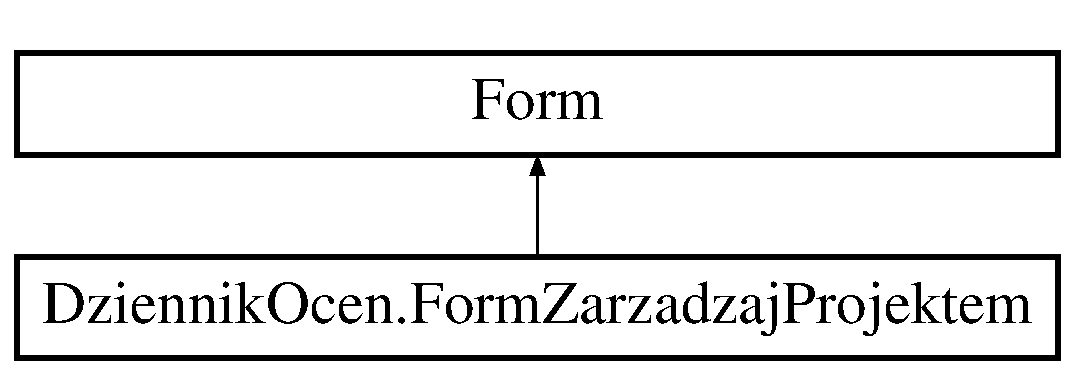
\includegraphics[height=2.000000cm]{class_dziennik_ocen_1_1_form_zarzadzaj_projektem}
\end{center}
\end{figure}
\subsection*{Public Member Functions}
\begin{DoxyCompactItemize}
\item 
\hyperlink{class_dziennik_ocen_1_1_form_zarzadzaj_projektem_ab02c6928f43c0339196925863d7553aa}{Form\+Zarzadzaj\+Projektem} (\hyperlink{class_dziennik_ocen_1_1projekty}{projekty} \hyperlink{class_dziennik_ocen_1_1_form_zarzadzaj_projektem_ad28eeefcf293cabe18ed034de6f7b9b9}{projekt})
\end{DoxyCompactItemize}
\subsection*{Protected Member Functions}
\begin{DoxyCompactItemize}
\item 
override void \hyperlink{class_dziennik_ocen_1_1_form_zarzadzaj_projektem_ac03323290cf11c8dbd8d88703dca9b0f}{Dispose} (bool disposing)
\begin{DoxyCompactList}\small\item\em Clean up any resources being used. \end{DoxyCompactList}\end{DoxyCompactItemize}
\subsection*{Properties}
\begin{DoxyCompactItemize}
\item 
\hyperlink{class_dziennik_ocen_1_1projekty}{projekty} \hyperlink{class_dziennik_ocen_1_1_form_zarzadzaj_projektem_a34aa59a4cb2a97b1a8f864775d250d45}{Projekt}\hspace{0.3cm}{\ttfamily  \mbox{[}get, set\mbox{]}}
\end{DoxyCompactItemize}
\subsection*{Private Member Functions}
\begin{DoxyCompactItemize}
\item 
void \hyperlink{class_dziennik_ocen_1_1_form_zarzadzaj_projektem_a903734712c2bc1345ff56fe786a96e22}{btn\+Zapisz\+\_\+\+Click} (object sender, Event\+Args e)
\item 
void \hyperlink{class_dziennik_ocen_1_1_form_zarzadzaj_projektem_a9531760113ecca03261970889c094c96}{Initialize\+Component} ()
\begin{DoxyCompactList}\small\item\em Required method for Designer support -\/ do not modify the contents of this method with the code editor. \end{DoxyCompactList}\end{DoxyCompactItemize}
\subsection*{Private Attributes}
\begin{DoxyCompactItemize}
\item 
\hyperlink{class_dziennik_ocen_1_1projekty}{projekty} \hyperlink{class_dziennik_ocen_1_1_form_zarzadzaj_projektem_ad28eeefcf293cabe18ed034de6f7b9b9}{projekt}
\item 
\hyperlink{class_dziennik_ocen_1_1_dziennik_ocen_entities}{Dziennik\+Ocen\+Entities} \hyperlink{class_dziennik_ocen_1_1_form_zarzadzaj_projektem_a2db3713590e45e56a37c3b7220b6453c}{db} = new \hyperlink{class_dziennik_ocen_1_1_dziennik_ocen_entities}{Dziennik\+Ocen\+Entities}()
\item 
System.\+Component\+Model.\+I\+Container \hyperlink{class_dziennik_ocen_1_1_form_zarzadzaj_projektem_a6e97af0a821e84d1bc6aea234de2d443}{components} = null
\begin{DoxyCompactList}\small\item\em Required designer variable. \end{DoxyCompactList}\item 
System.\+Windows.\+Forms.\+Text\+Box \hyperlink{class_dziennik_ocen_1_1_form_zarzadzaj_projektem_a3c52e78830d152bcd9687d57d2f73dd0}{tbx\+Ocena}
\item 
System.\+Windows.\+Forms.\+Label \hyperlink{class_dziennik_ocen_1_1_form_zarzadzaj_projektem_ae6542c6fd11a611106ab7f0cd3640ebf}{label1}
\item 
System.\+Windows.\+Forms.\+Label \hyperlink{class_dziennik_ocen_1_1_form_zarzadzaj_projektem_a3eedf20c866486ca2910dd519d28bb31}{label2}
\item 
System.\+Windows.\+Forms.\+Label \hyperlink{class_dziennik_ocen_1_1_form_zarzadzaj_projektem_a1662ef206e960bcb8bb903c0b8335094}{label3}
\item 
System.\+Windows.\+Forms.\+Text\+Box \hyperlink{class_dziennik_ocen_1_1_form_zarzadzaj_projektem_aa8803c03bc8917991c70877a55c3f30a}{tbx\+Data}
\item 
System.\+Windows.\+Forms.\+Text\+Box \hyperlink{class_dziennik_ocen_1_1_form_zarzadzaj_projektem_ac1bfcac93cf76188c272dee28a136238}{tbx\+Uwagi}
\item 
System.\+Windows.\+Forms.\+Button \hyperlink{class_dziennik_ocen_1_1_form_zarzadzaj_projektem_abf06a8fd2ddc8622e1f3310250bf8fdc}{btn\+Anuluj}
\item 
System.\+Windows.\+Forms.\+Button \hyperlink{class_dziennik_ocen_1_1_form_zarzadzaj_projektem_acce0d9c3197e6545fef245a6729baa41}{btn\+Zapisz}
\end{DoxyCompactItemize}


\subsection{Constructor \& Destructor Documentation}
\mbox{\Hypertarget{class_dziennik_ocen_1_1_form_zarzadzaj_projektem_ab02c6928f43c0339196925863d7553aa}\label{class_dziennik_ocen_1_1_form_zarzadzaj_projektem_ab02c6928f43c0339196925863d7553aa}} 
\index{Dziennik\+Ocen\+::\+Form\+Zarzadzaj\+Projektem@{Dziennik\+Ocen\+::\+Form\+Zarzadzaj\+Projektem}!Form\+Zarzadzaj\+Projektem@{Form\+Zarzadzaj\+Projektem}}
\index{Form\+Zarzadzaj\+Projektem@{Form\+Zarzadzaj\+Projektem}!Dziennik\+Ocen\+::\+Form\+Zarzadzaj\+Projektem@{Dziennik\+Ocen\+::\+Form\+Zarzadzaj\+Projektem}}
\subsubsection{\texorpdfstring{Form\+Zarzadzaj\+Projektem()}{FormZarzadzajProjektem()}}
{\footnotesize\ttfamily Dziennik\+Ocen.\+Form\+Zarzadzaj\+Projektem.\+Form\+Zarzadzaj\+Projektem (\begin{DoxyParamCaption}\item[{\hyperlink{class_dziennik_ocen_1_1projekty}{projekty}}]{projekt }\end{DoxyParamCaption})\hspace{0.3cm}{\ttfamily [inline]}}



\subsection{Member Function Documentation}
\mbox{\Hypertarget{class_dziennik_ocen_1_1_form_zarzadzaj_projektem_a903734712c2bc1345ff56fe786a96e22}\label{class_dziennik_ocen_1_1_form_zarzadzaj_projektem_a903734712c2bc1345ff56fe786a96e22}} 
\index{Dziennik\+Ocen\+::\+Form\+Zarzadzaj\+Projektem@{Dziennik\+Ocen\+::\+Form\+Zarzadzaj\+Projektem}!btn\+Zapisz\+\_\+\+Click@{btn\+Zapisz\+\_\+\+Click}}
\index{btn\+Zapisz\+\_\+\+Click@{btn\+Zapisz\+\_\+\+Click}!Dziennik\+Ocen\+::\+Form\+Zarzadzaj\+Projektem@{Dziennik\+Ocen\+::\+Form\+Zarzadzaj\+Projektem}}
\subsubsection{\texorpdfstring{btn\+Zapisz\+\_\+\+Click()}{btnZapisz\_Click()}}
{\footnotesize\ttfamily void Dziennik\+Ocen.\+Form\+Zarzadzaj\+Projektem.\+btn\+Zapisz\+\_\+\+Click (\begin{DoxyParamCaption}\item[{object}]{sender,  }\item[{Event\+Args}]{e }\end{DoxyParamCaption})\hspace{0.3cm}{\ttfamily [inline]}, {\ttfamily [private]}}

\mbox{\Hypertarget{class_dziennik_ocen_1_1_form_zarzadzaj_projektem_ac03323290cf11c8dbd8d88703dca9b0f}\label{class_dziennik_ocen_1_1_form_zarzadzaj_projektem_ac03323290cf11c8dbd8d88703dca9b0f}} 
\index{Dziennik\+Ocen\+::\+Form\+Zarzadzaj\+Projektem@{Dziennik\+Ocen\+::\+Form\+Zarzadzaj\+Projektem}!Dispose@{Dispose}}
\index{Dispose@{Dispose}!Dziennik\+Ocen\+::\+Form\+Zarzadzaj\+Projektem@{Dziennik\+Ocen\+::\+Form\+Zarzadzaj\+Projektem}}
\subsubsection{\texorpdfstring{Dispose()}{Dispose()}}
{\footnotesize\ttfamily override void Dziennik\+Ocen.\+Form\+Zarzadzaj\+Projektem.\+Dispose (\begin{DoxyParamCaption}\item[{bool}]{disposing }\end{DoxyParamCaption})\hspace{0.3cm}{\ttfamily [inline]}, {\ttfamily [protected]}}



Clean up any resources being used. 


\begin{DoxyParams}{Parameters}
{\em disposing} & true if managed resources should be disposed; otherwise, false.\\
\hline
\end{DoxyParams}
\mbox{\Hypertarget{class_dziennik_ocen_1_1_form_zarzadzaj_projektem_a9531760113ecca03261970889c094c96}\label{class_dziennik_ocen_1_1_form_zarzadzaj_projektem_a9531760113ecca03261970889c094c96}} 
\index{Dziennik\+Ocen\+::\+Form\+Zarzadzaj\+Projektem@{Dziennik\+Ocen\+::\+Form\+Zarzadzaj\+Projektem}!Initialize\+Component@{Initialize\+Component}}
\index{Initialize\+Component@{Initialize\+Component}!Dziennik\+Ocen\+::\+Form\+Zarzadzaj\+Projektem@{Dziennik\+Ocen\+::\+Form\+Zarzadzaj\+Projektem}}
\subsubsection{\texorpdfstring{Initialize\+Component()}{InitializeComponent()}}
{\footnotesize\ttfamily void Dziennik\+Ocen.\+Form\+Zarzadzaj\+Projektem.\+Initialize\+Component (\begin{DoxyParamCaption}{ }\end{DoxyParamCaption})\hspace{0.3cm}{\ttfamily [inline]}, {\ttfamily [private]}}



Required method for Designer support -\/ do not modify the contents of this method with the code editor. 



\subsection{Member Data Documentation}
\mbox{\Hypertarget{class_dziennik_ocen_1_1_form_zarzadzaj_projektem_abf06a8fd2ddc8622e1f3310250bf8fdc}\label{class_dziennik_ocen_1_1_form_zarzadzaj_projektem_abf06a8fd2ddc8622e1f3310250bf8fdc}} 
\index{Dziennik\+Ocen\+::\+Form\+Zarzadzaj\+Projektem@{Dziennik\+Ocen\+::\+Form\+Zarzadzaj\+Projektem}!btn\+Anuluj@{btn\+Anuluj}}
\index{btn\+Anuluj@{btn\+Anuluj}!Dziennik\+Ocen\+::\+Form\+Zarzadzaj\+Projektem@{Dziennik\+Ocen\+::\+Form\+Zarzadzaj\+Projektem}}
\subsubsection{\texorpdfstring{btn\+Anuluj}{btnAnuluj}}
{\footnotesize\ttfamily System.\+Windows.\+Forms.\+Button Dziennik\+Ocen.\+Form\+Zarzadzaj\+Projektem.\+btn\+Anuluj\hspace{0.3cm}{\ttfamily [private]}}

\mbox{\Hypertarget{class_dziennik_ocen_1_1_form_zarzadzaj_projektem_acce0d9c3197e6545fef245a6729baa41}\label{class_dziennik_ocen_1_1_form_zarzadzaj_projektem_acce0d9c3197e6545fef245a6729baa41}} 
\index{Dziennik\+Ocen\+::\+Form\+Zarzadzaj\+Projektem@{Dziennik\+Ocen\+::\+Form\+Zarzadzaj\+Projektem}!btn\+Zapisz@{btn\+Zapisz}}
\index{btn\+Zapisz@{btn\+Zapisz}!Dziennik\+Ocen\+::\+Form\+Zarzadzaj\+Projektem@{Dziennik\+Ocen\+::\+Form\+Zarzadzaj\+Projektem}}
\subsubsection{\texorpdfstring{btn\+Zapisz}{btnZapisz}}
{\footnotesize\ttfamily System.\+Windows.\+Forms.\+Button Dziennik\+Ocen.\+Form\+Zarzadzaj\+Projektem.\+btn\+Zapisz\hspace{0.3cm}{\ttfamily [private]}}

\mbox{\Hypertarget{class_dziennik_ocen_1_1_form_zarzadzaj_projektem_a6e97af0a821e84d1bc6aea234de2d443}\label{class_dziennik_ocen_1_1_form_zarzadzaj_projektem_a6e97af0a821e84d1bc6aea234de2d443}} 
\index{Dziennik\+Ocen\+::\+Form\+Zarzadzaj\+Projektem@{Dziennik\+Ocen\+::\+Form\+Zarzadzaj\+Projektem}!components@{components}}
\index{components@{components}!Dziennik\+Ocen\+::\+Form\+Zarzadzaj\+Projektem@{Dziennik\+Ocen\+::\+Form\+Zarzadzaj\+Projektem}}
\subsubsection{\texorpdfstring{components}{components}}
{\footnotesize\ttfamily System.\+Component\+Model.\+I\+Container Dziennik\+Ocen.\+Form\+Zarzadzaj\+Projektem.\+components = null\hspace{0.3cm}{\ttfamily [private]}}



Required designer variable. 

\mbox{\Hypertarget{class_dziennik_ocen_1_1_form_zarzadzaj_projektem_a2db3713590e45e56a37c3b7220b6453c}\label{class_dziennik_ocen_1_1_form_zarzadzaj_projektem_a2db3713590e45e56a37c3b7220b6453c}} 
\index{Dziennik\+Ocen\+::\+Form\+Zarzadzaj\+Projektem@{Dziennik\+Ocen\+::\+Form\+Zarzadzaj\+Projektem}!db@{db}}
\index{db@{db}!Dziennik\+Ocen\+::\+Form\+Zarzadzaj\+Projektem@{Dziennik\+Ocen\+::\+Form\+Zarzadzaj\+Projektem}}
\subsubsection{\texorpdfstring{db}{db}}
{\footnotesize\ttfamily \hyperlink{class_dziennik_ocen_1_1_dziennik_ocen_entities}{Dziennik\+Ocen\+Entities} Dziennik\+Ocen.\+Form\+Zarzadzaj\+Projektem.\+db = new \hyperlink{class_dziennik_ocen_1_1_dziennik_ocen_entities}{Dziennik\+Ocen\+Entities}()\hspace{0.3cm}{\ttfamily [private]}}

\mbox{\Hypertarget{class_dziennik_ocen_1_1_form_zarzadzaj_projektem_ae6542c6fd11a611106ab7f0cd3640ebf}\label{class_dziennik_ocen_1_1_form_zarzadzaj_projektem_ae6542c6fd11a611106ab7f0cd3640ebf}} 
\index{Dziennik\+Ocen\+::\+Form\+Zarzadzaj\+Projektem@{Dziennik\+Ocen\+::\+Form\+Zarzadzaj\+Projektem}!label1@{label1}}
\index{label1@{label1}!Dziennik\+Ocen\+::\+Form\+Zarzadzaj\+Projektem@{Dziennik\+Ocen\+::\+Form\+Zarzadzaj\+Projektem}}
\subsubsection{\texorpdfstring{label1}{label1}}
{\footnotesize\ttfamily System.\+Windows.\+Forms.\+Label Dziennik\+Ocen.\+Form\+Zarzadzaj\+Projektem.\+label1\hspace{0.3cm}{\ttfamily [private]}}

\mbox{\Hypertarget{class_dziennik_ocen_1_1_form_zarzadzaj_projektem_a3eedf20c866486ca2910dd519d28bb31}\label{class_dziennik_ocen_1_1_form_zarzadzaj_projektem_a3eedf20c866486ca2910dd519d28bb31}} 
\index{Dziennik\+Ocen\+::\+Form\+Zarzadzaj\+Projektem@{Dziennik\+Ocen\+::\+Form\+Zarzadzaj\+Projektem}!label2@{label2}}
\index{label2@{label2}!Dziennik\+Ocen\+::\+Form\+Zarzadzaj\+Projektem@{Dziennik\+Ocen\+::\+Form\+Zarzadzaj\+Projektem}}
\subsubsection{\texorpdfstring{label2}{label2}}
{\footnotesize\ttfamily System.\+Windows.\+Forms.\+Label Dziennik\+Ocen.\+Form\+Zarzadzaj\+Projektem.\+label2\hspace{0.3cm}{\ttfamily [private]}}

\mbox{\Hypertarget{class_dziennik_ocen_1_1_form_zarzadzaj_projektem_a1662ef206e960bcb8bb903c0b8335094}\label{class_dziennik_ocen_1_1_form_zarzadzaj_projektem_a1662ef206e960bcb8bb903c0b8335094}} 
\index{Dziennik\+Ocen\+::\+Form\+Zarzadzaj\+Projektem@{Dziennik\+Ocen\+::\+Form\+Zarzadzaj\+Projektem}!label3@{label3}}
\index{label3@{label3}!Dziennik\+Ocen\+::\+Form\+Zarzadzaj\+Projektem@{Dziennik\+Ocen\+::\+Form\+Zarzadzaj\+Projektem}}
\subsubsection{\texorpdfstring{label3}{label3}}
{\footnotesize\ttfamily System.\+Windows.\+Forms.\+Label Dziennik\+Ocen.\+Form\+Zarzadzaj\+Projektem.\+label3\hspace{0.3cm}{\ttfamily [private]}}

\mbox{\Hypertarget{class_dziennik_ocen_1_1_form_zarzadzaj_projektem_ad28eeefcf293cabe18ed034de6f7b9b9}\label{class_dziennik_ocen_1_1_form_zarzadzaj_projektem_ad28eeefcf293cabe18ed034de6f7b9b9}} 
\index{Dziennik\+Ocen\+::\+Form\+Zarzadzaj\+Projektem@{Dziennik\+Ocen\+::\+Form\+Zarzadzaj\+Projektem}!projekt@{projekt}}
\index{projekt@{projekt}!Dziennik\+Ocen\+::\+Form\+Zarzadzaj\+Projektem@{Dziennik\+Ocen\+::\+Form\+Zarzadzaj\+Projektem}}
\subsubsection{\texorpdfstring{projekt}{projekt}}
{\footnotesize\ttfamily \hyperlink{class_dziennik_ocen_1_1projekty}{projekty} Dziennik\+Ocen.\+Form\+Zarzadzaj\+Projektem.\+projekt\hspace{0.3cm}{\ttfamily [private]}}

\mbox{\Hypertarget{class_dziennik_ocen_1_1_form_zarzadzaj_projektem_aa8803c03bc8917991c70877a55c3f30a}\label{class_dziennik_ocen_1_1_form_zarzadzaj_projektem_aa8803c03bc8917991c70877a55c3f30a}} 
\index{Dziennik\+Ocen\+::\+Form\+Zarzadzaj\+Projektem@{Dziennik\+Ocen\+::\+Form\+Zarzadzaj\+Projektem}!tbx\+Data@{tbx\+Data}}
\index{tbx\+Data@{tbx\+Data}!Dziennik\+Ocen\+::\+Form\+Zarzadzaj\+Projektem@{Dziennik\+Ocen\+::\+Form\+Zarzadzaj\+Projektem}}
\subsubsection{\texorpdfstring{tbx\+Data}{tbxData}}
{\footnotesize\ttfamily System.\+Windows.\+Forms.\+Text\+Box Dziennik\+Ocen.\+Form\+Zarzadzaj\+Projektem.\+tbx\+Data\hspace{0.3cm}{\ttfamily [private]}}

\mbox{\Hypertarget{class_dziennik_ocen_1_1_form_zarzadzaj_projektem_a3c52e78830d152bcd9687d57d2f73dd0}\label{class_dziennik_ocen_1_1_form_zarzadzaj_projektem_a3c52e78830d152bcd9687d57d2f73dd0}} 
\index{Dziennik\+Ocen\+::\+Form\+Zarzadzaj\+Projektem@{Dziennik\+Ocen\+::\+Form\+Zarzadzaj\+Projektem}!tbx\+Ocena@{tbx\+Ocena}}
\index{tbx\+Ocena@{tbx\+Ocena}!Dziennik\+Ocen\+::\+Form\+Zarzadzaj\+Projektem@{Dziennik\+Ocen\+::\+Form\+Zarzadzaj\+Projektem}}
\subsubsection{\texorpdfstring{tbx\+Ocena}{tbxOcena}}
{\footnotesize\ttfamily System.\+Windows.\+Forms.\+Text\+Box Dziennik\+Ocen.\+Form\+Zarzadzaj\+Projektem.\+tbx\+Ocena\hspace{0.3cm}{\ttfamily [private]}}

\mbox{\Hypertarget{class_dziennik_ocen_1_1_form_zarzadzaj_projektem_ac1bfcac93cf76188c272dee28a136238}\label{class_dziennik_ocen_1_1_form_zarzadzaj_projektem_ac1bfcac93cf76188c272dee28a136238}} 
\index{Dziennik\+Ocen\+::\+Form\+Zarzadzaj\+Projektem@{Dziennik\+Ocen\+::\+Form\+Zarzadzaj\+Projektem}!tbx\+Uwagi@{tbx\+Uwagi}}
\index{tbx\+Uwagi@{tbx\+Uwagi}!Dziennik\+Ocen\+::\+Form\+Zarzadzaj\+Projektem@{Dziennik\+Ocen\+::\+Form\+Zarzadzaj\+Projektem}}
\subsubsection{\texorpdfstring{tbx\+Uwagi}{tbxUwagi}}
{\footnotesize\ttfamily System.\+Windows.\+Forms.\+Text\+Box Dziennik\+Ocen.\+Form\+Zarzadzaj\+Projektem.\+tbx\+Uwagi\hspace{0.3cm}{\ttfamily [private]}}



\subsection{Property Documentation}
\mbox{\Hypertarget{class_dziennik_ocen_1_1_form_zarzadzaj_projektem_a34aa59a4cb2a97b1a8f864775d250d45}\label{class_dziennik_ocen_1_1_form_zarzadzaj_projektem_a34aa59a4cb2a97b1a8f864775d250d45}} 
\index{Dziennik\+Ocen\+::\+Form\+Zarzadzaj\+Projektem@{Dziennik\+Ocen\+::\+Form\+Zarzadzaj\+Projektem}!Projekt@{Projekt}}
\index{Projekt@{Projekt}!Dziennik\+Ocen\+::\+Form\+Zarzadzaj\+Projektem@{Dziennik\+Ocen\+::\+Form\+Zarzadzaj\+Projektem}}
\subsubsection{\texorpdfstring{Projekt}{Projekt}}
{\footnotesize\ttfamily \hyperlink{class_dziennik_ocen_1_1projekty}{projekty} Dziennik\+Ocen.\+Form\+Zarzadzaj\+Projektem.\+Projekt\hspace{0.3cm}{\ttfamily [get]}, {\ttfamily [set]}}



The documentation for this class was generated from the following files\+:\begin{DoxyCompactItemize}
\item 
Dziennik\+Ocen/\hyperlink{_form_zarzadzaj_projektem_8cs}{Form\+Zarzadzaj\+Projektem.\+cs}\item 
Dziennik\+Ocen/\hyperlink{_form_zarzadzaj_projektem_8_designer_8cs}{Form\+Zarzadzaj\+Projektem.\+Designer.\+cs}\end{DoxyCompactItemize}

\hypertarget{class_dziennik_ocen_1_1_form_zarzadzaj_studentem}{}\section{Dziennik\+Ocen.\+Form\+Zarzadzaj\+Studentem Class Reference}
\label{class_dziennik_ocen_1_1_form_zarzadzaj_studentem}\index{Dziennik\+Ocen.\+Form\+Zarzadzaj\+Studentem@{Dziennik\+Ocen.\+Form\+Zarzadzaj\+Studentem}}
Inheritance diagram for Dziennik\+Ocen.\+Form\+Zarzadzaj\+Studentem\+:\begin{figure}[H]
\begin{center}
\leavevmode
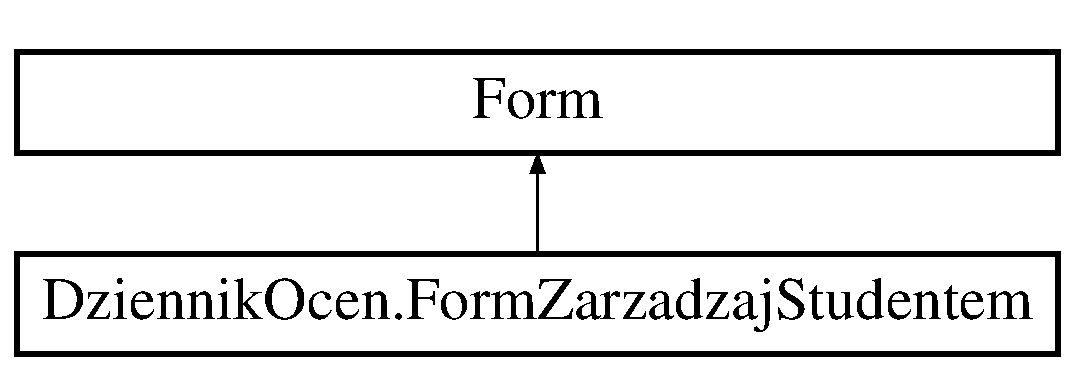
\includegraphics[height=2.000000cm]{class_dziennik_ocen_1_1_form_zarzadzaj_studentem}
\end{center}
\end{figure}
\subsection*{Public Member Functions}
\begin{DoxyCompactItemize}
\item 
\hyperlink{class_dziennik_ocen_1_1_form_zarzadzaj_studentem_a2437cda216a51a08ae749edb555e8b28}{Form\+Zarzadzaj\+Studentem} (\hyperlink{class_dziennik_ocen_1_1_s_t_u_d_e_n_t}{S\+T\+U\+D\+E\+NT} \hyperlink{class_dziennik_ocen_1_1_form_zarzadzaj_studentem_af05f1e588d74d7907c8259468f916dad}{student}, I\+List$<$ \hyperlink{class_dziennik_ocen_1_1_g_r_u_p_a}{G\+R\+U\+PA} $>$ \hyperlink{class_dziennik_ocen_1_1_g_r_u_p_a}{G\+R\+U\+PA})
\end{DoxyCompactItemize}
\subsection*{Protected Member Functions}
\begin{DoxyCompactItemize}
\item 
override void \hyperlink{class_dziennik_ocen_1_1_form_zarzadzaj_studentem_a90df6d8bdf00f5ce184053c526952368}{Dispose} (bool disposing)
\begin{DoxyCompactList}\small\item\em Clean up any resources being used. \end{DoxyCompactList}\end{DoxyCompactItemize}
\subsection*{Properties}
\begin{DoxyCompactItemize}
\item 
\hyperlink{class_dziennik_ocen_1_1_s_t_u_d_e_n_t}{S\+T\+U\+D\+E\+NT} \hyperlink{class_dziennik_ocen_1_1_form_zarzadzaj_studentem_a6725e64848d2a943830083be3849c3e5}{Student}\hspace{0.3cm}{\ttfamily  \mbox{[}get, set\mbox{]}}
\end{DoxyCompactItemize}
\subsection*{Private Member Functions}
\begin{DoxyCompactItemize}
\item 
void \hyperlink{class_dziennik_ocen_1_1_form_zarzadzaj_studentem_afbd85dca33ecb88bc7498002ccaed41e}{Form\+Zarzadzaj\+Studentem\+\_\+\+Load} (object sender, Event\+Args e)
\item 
void \hyperlink{class_dziennik_ocen_1_1_form_zarzadzaj_studentem_a7aaf60fcd65bc83c851ddac85076a5dd}{btn\+Zapisz\+\_\+\+Click} (object sender, Event\+Args e)
\item 
void \hyperlink{class_dziennik_ocen_1_1_form_zarzadzaj_studentem_a9236e2f084822188d36dac89e165ff5b}{Initialize\+Component} ()
\begin{DoxyCompactList}\small\item\em Required method for Designer support -\/ do not modify the contents of this method with the code editor. \end{DoxyCompactList}\end{DoxyCompactItemize}
\subsection*{Private Attributes}
\begin{DoxyCompactItemize}
\item 
\hyperlink{class_dziennik_ocen_1_1_s_t_u_d_e_n_t}{S\+T\+U\+D\+E\+NT} \hyperlink{class_dziennik_ocen_1_1_form_zarzadzaj_studentem_af05f1e588d74d7907c8259468f916dad}{student}
\item 
System.\+Component\+Model.\+I\+Container \hyperlink{class_dziennik_ocen_1_1_form_zarzadzaj_studentem_a541f772925213cefc818120c1b07049e}{components} = null
\begin{DoxyCompactList}\small\item\em Required designer variable. \end{DoxyCompactList}\item 
System.\+Windows.\+Forms.\+Combo\+Box \hyperlink{class_dziennik_ocen_1_1_form_zarzadzaj_studentem_aa214491bf19dacbdff01bcc4d990b590}{cbx\+Grupa}
\item 
System.\+Windows.\+Forms.\+Text\+Box \hyperlink{class_dziennik_ocen_1_1_form_zarzadzaj_studentem_af49d6f5fc0b260c4adf8fc04e648b7de}{tbx\+Imie}
\item 
System.\+Windows.\+Forms.\+Text\+Box \hyperlink{class_dziennik_ocen_1_1_form_zarzadzaj_studentem_afcd8cf8e73a3262cb6f5bd0568be124f}{tbx\+Nazwisko}
\item 
System.\+Windows.\+Forms.\+Text\+Box \hyperlink{class_dziennik_ocen_1_1_form_zarzadzaj_studentem_ab6cac96deb278395b902bbbe671e580e}{tbx\+Telefon}
\item 
System.\+Windows.\+Forms.\+Text\+Box \hyperlink{class_dziennik_ocen_1_1_form_zarzadzaj_studentem_a4e89770014619d2cf01ae4d1051de038}{tbx\+Adres}
\item 
System.\+Windows.\+Forms.\+Text\+Box \hyperlink{class_dziennik_ocen_1_1_form_zarzadzaj_studentem_a159ebcfb51180c03036cefb6115301d8}{tbx\+Email}
\item 
System.\+Windows.\+Forms.\+Label \hyperlink{class_dziennik_ocen_1_1_form_zarzadzaj_studentem_a0b612309ffc8bf140467767bed9e894b}{lbl\+Grupa}
\item 
System.\+Windows.\+Forms.\+Label \hyperlink{class_dziennik_ocen_1_1_form_zarzadzaj_studentem_a9ddbf901bf5e98578df9ed264f83484f}{lbl\+Imie}
\item 
System.\+Windows.\+Forms.\+Label \hyperlink{class_dziennik_ocen_1_1_form_zarzadzaj_studentem_a8989cb2dcf05fabf7648d94e52c1da4f}{lbl\+Nazwisko}
\item 
System.\+Windows.\+Forms.\+Label \hyperlink{class_dziennik_ocen_1_1_form_zarzadzaj_studentem_a44a5cb8264b5afe2cf830b996fc6c005}{lbl\+Email}
\item 
System.\+Windows.\+Forms.\+Label \hyperlink{class_dziennik_ocen_1_1_form_zarzadzaj_studentem_a0d41096de98b53d58817064c21408cec}{lbl\+Adres}
\item 
System.\+Windows.\+Forms.\+Label \hyperlink{class_dziennik_ocen_1_1_form_zarzadzaj_studentem_a8d890775b92e88eddf4e726e7fd715d1}{lbl\+Telefon}
\item 
System.\+Windows.\+Forms.\+Button \hyperlink{class_dziennik_ocen_1_1_form_zarzadzaj_studentem_aaa007386b53a7c157e97fbfcd6375697}{btn\+Zapisz}
\item 
System.\+Windows.\+Forms.\+Button \hyperlink{class_dziennik_ocen_1_1_form_zarzadzaj_studentem_aaf2b7d143a88c7eca727c9d07fe173e5}{btn\+Anuluj}
\item 
System.\+Windows.\+Forms.\+Binding\+Source \hyperlink{class_dziennik_ocen_1_1_form_zarzadzaj_studentem_a69189dd9447d5adfea2153e6cf1c1276}{bs\+G\+R\+U\+PA}
\end{DoxyCompactItemize}


\subsection{Constructor \& Destructor Documentation}
\mbox{\Hypertarget{class_dziennik_ocen_1_1_form_zarzadzaj_studentem_a2437cda216a51a08ae749edb555e8b28}\label{class_dziennik_ocen_1_1_form_zarzadzaj_studentem_a2437cda216a51a08ae749edb555e8b28}} 
\index{Dziennik\+Ocen\+::\+Form\+Zarzadzaj\+Studentem@{Dziennik\+Ocen\+::\+Form\+Zarzadzaj\+Studentem}!Form\+Zarzadzaj\+Studentem@{Form\+Zarzadzaj\+Studentem}}
\index{Form\+Zarzadzaj\+Studentem@{Form\+Zarzadzaj\+Studentem}!Dziennik\+Ocen\+::\+Form\+Zarzadzaj\+Studentem@{Dziennik\+Ocen\+::\+Form\+Zarzadzaj\+Studentem}}
\subsubsection{\texorpdfstring{Form\+Zarzadzaj\+Studentem()}{FormZarzadzajStudentem()}}
{\footnotesize\ttfamily Dziennik\+Ocen.\+Form\+Zarzadzaj\+Studentem.\+Form\+Zarzadzaj\+Studentem (\begin{DoxyParamCaption}\item[{\hyperlink{class_dziennik_ocen_1_1_s_t_u_d_e_n_t}{S\+T\+U\+D\+E\+NT}}]{student,  }\item[{I\+List$<$ \hyperlink{class_dziennik_ocen_1_1_g_r_u_p_a}{G\+R\+U\+PA} $>$}]{G\+R\+U\+PA }\end{DoxyParamCaption})\hspace{0.3cm}{\ttfamily [inline]}}



\subsection{Member Function Documentation}
\mbox{\Hypertarget{class_dziennik_ocen_1_1_form_zarzadzaj_studentem_a7aaf60fcd65bc83c851ddac85076a5dd}\label{class_dziennik_ocen_1_1_form_zarzadzaj_studentem_a7aaf60fcd65bc83c851ddac85076a5dd}} 
\index{Dziennik\+Ocen\+::\+Form\+Zarzadzaj\+Studentem@{Dziennik\+Ocen\+::\+Form\+Zarzadzaj\+Studentem}!btn\+Zapisz\+\_\+\+Click@{btn\+Zapisz\+\_\+\+Click}}
\index{btn\+Zapisz\+\_\+\+Click@{btn\+Zapisz\+\_\+\+Click}!Dziennik\+Ocen\+::\+Form\+Zarzadzaj\+Studentem@{Dziennik\+Ocen\+::\+Form\+Zarzadzaj\+Studentem}}
\subsubsection{\texorpdfstring{btn\+Zapisz\+\_\+\+Click()}{btnZapisz\_Click()}}
{\footnotesize\ttfamily void Dziennik\+Ocen.\+Form\+Zarzadzaj\+Studentem.\+btn\+Zapisz\+\_\+\+Click (\begin{DoxyParamCaption}\item[{object}]{sender,  }\item[{Event\+Args}]{e }\end{DoxyParamCaption})\hspace{0.3cm}{\ttfamily [inline]}, {\ttfamily [private]}}

\mbox{\Hypertarget{class_dziennik_ocen_1_1_form_zarzadzaj_studentem_a90df6d8bdf00f5ce184053c526952368}\label{class_dziennik_ocen_1_1_form_zarzadzaj_studentem_a90df6d8bdf00f5ce184053c526952368}} 
\index{Dziennik\+Ocen\+::\+Form\+Zarzadzaj\+Studentem@{Dziennik\+Ocen\+::\+Form\+Zarzadzaj\+Studentem}!Dispose@{Dispose}}
\index{Dispose@{Dispose}!Dziennik\+Ocen\+::\+Form\+Zarzadzaj\+Studentem@{Dziennik\+Ocen\+::\+Form\+Zarzadzaj\+Studentem}}
\subsubsection{\texorpdfstring{Dispose()}{Dispose()}}
{\footnotesize\ttfamily override void Dziennik\+Ocen.\+Form\+Zarzadzaj\+Studentem.\+Dispose (\begin{DoxyParamCaption}\item[{bool}]{disposing }\end{DoxyParamCaption})\hspace{0.3cm}{\ttfamily [inline]}, {\ttfamily [protected]}}



Clean up any resources being used. 


\begin{DoxyParams}{Parameters}
{\em disposing} & true if managed resources should be disposed; otherwise, false.\\
\hline
\end{DoxyParams}
\mbox{\Hypertarget{class_dziennik_ocen_1_1_form_zarzadzaj_studentem_afbd85dca33ecb88bc7498002ccaed41e}\label{class_dziennik_ocen_1_1_form_zarzadzaj_studentem_afbd85dca33ecb88bc7498002ccaed41e}} 
\index{Dziennik\+Ocen\+::\+Form\+Zarzadzaj\+Studentem@{Dziennik\+Ocen\+::\+Form\+Zarzadzaj\+Studentem}!Form\+Zarzadzaj\+Studentem\+\_\+\+Load@{Form\+Zarzadzaj\+Studentem\+\_\+\+Load}}
\index{Form\+Zarzadzaj\+Studentem\+\_\+\+Load@{Form\+Zarzadzaj\+Studentem\+\_\+\+Load}!Dziennik\+Ocen\+::\+Form\+Zarzadzaj\+Studentem@{Dziennik\+Ocen\+::\+Form\+Zarzadzaj\+Studentem}}
\subsubsection{\texorpdfstring{Form\+Zarzadzaj\+Studentem\+\_\+\+Load()}{FormZarzadzajStudentem\_Load()}}
{\footnotesize\ttfamily void Dziennik\+Ocen.\+Form\+Zarzadzaj\+Studentem.\+Form\+Zarzadzaj\+Studentem\+\_\+\+Load (\begin{DoxyParamCaption}\item[{object}]{sender,  }\item[{Event\+Args}]{e }\end{DoxyParamCaption})\hspace{0.3cm}{\ttfamily [inline]}, {\ttfamily [private]}}

\mbox{\Hypertarget{class_dziennik_ocen_1_1_form_zarzadzaj_studentem_a9236e2f084822188d36dac89e165ff5b}\label{class_dziennik_ocen_1_1_form_zarzadzaj_studentem_a9236e2f084822188d36dac89e165ff5b}} 
\index{Dziennik\+Ocen\+::\+Form\+Zarzadzaj\+Studentem@{Dziennik\+Ocen\+::\+Form\+Zarzadzaj\+Studentem}!Initialize\+Component@{Initialize\+Component}}
\index{Initialize\+Component@{Initialize\+Component}!Dziennik\+Ocen\+::\+Form\+Zarzadzaj\+Studentem@{Dziennik\+Ocen\+::\+Form\+Zarzadzaj\+Studentem}}
\subsubsection{\texorpdfstring{Initialize\+Component()}{InitializeComponent()}}
{\footnotesize\ttfamily void Dziennik\+Ocen.\+Form\+Zarzadzaj\+Studentem.\+Initialize\+Component (\begin{DoxyParamCaption}{ }\end{DoxyParamCaption})\hspace{0.3cm}{\ttfamily [inline]}, {\ttfamily [private]}}



Required method for Designer support -\/ do not modify the contents of this method with the code editor. 



\subsection{Member Data Documentation}
\mbox{\Hypertarget{class_dziennik_ocen_1_1_form_zarzadzaj_studentem_a69189dd9447d5adfea2153e6cf1c1276}\label{class_dziennik_ocen_1_1_form_zarzadzaj_studentem_a69189dd9447d5adfea2153e6cf1c1276}} 
\index{Dziennik\+Ocen\+::\+Form\+Zarzadzaj\+Studentem@{Dziennik\+Ocen\+::\+Form\+Zarzadzaj\+Studentem}!bs\+G\+R\+U\+PA@{bs\+G\+R\+U\+PA}}
\index{bs\+G\+R\+U\+PA@{bs\+G\+R\+U\+PA}!Dziennik\+Ocen\+::\+Form\+Zarzadzaj\+Studentem@{Dziennik\+Ocen\+::\+Form\+Zarzadzaj\+Studentem}}
\subsubsection{\texorpdfstring{bs\+G\+R\+U\+PA}{bsGRUPA}}
{\footnotesize\ttfamily System.\+Windows.\+Forms.\+Binding\+Source Dziennik\+Ocen.\+Form\+Zarzadzaj\+Studentem.\+bs\+G\+R\+U\+PA\hspace{0.3cm}{\ttfamily [private]}}

\mbox{\Hypertarget{class_dziennik_ocen_1_1_form_zarzadzaj_studentem_aaf2b7d143a88c7eca727c9d07fe173e5}\label{class_dziennik_ocen_1_1_form_zarzadzaj_studentem_aaf2b7d143a88c7eca727c9d07fe173e5}} 
\index{Dziennik\+Ocen\+::\+Form\+Zarzadzaj\+Studentem@{Dziennik\+Ocen\+::\+Form\+Zarzadzaj\+Studentem}!btn\+Anuluj@{btn\+Anuluj}}
\index{btn\+Anuluj@{btn\+Anuluj}!Dziennik\+Ocen\+::\+Form\+Zarzadzaj\+Studentem@{Dziennik\+Ocen\+::\+Form\+Zarzadzaj\+Studentem}}
\subsubsection{\texorpdfstring{btn\+Anuluj}{btnAnuluj}}
{\footnotesize\ttfamily System.\+Windows.\+Forms.\+Button Dziennik\+Ocen.\+Form\+Zarzadzaj\+Studentem.\+btn\+Anuluj\hspace{0.3cm}{\ttfamily [private]}}

\mbox{\Hypertarget{class_dziennik_ocen_1_1_form_zarzadzaj_studentem_aaa007386b53a7c157e97fbfcd6375697}\label{class_dziennik_ocen_1_1_form_zarzadzaj_studentem_aaa007386b53a7c157e97fbfcd6375697}} 
\index{Dziennik\+Ocen\+::\+Form\+Zarzadzaj\+Studentem@{Dziennik\+Ocen\+::\+Form\+Zarzadzaj\+Studentem}!btn\+Zapisz@{btn\+Zapisz}}
\index{btn\+Zapisz@{btn\+Zapisz}!Dziennik\+Ocen\+::\+Form\+Zarzadzaj\+Studentem@{Dziennik\+Ocen\+::\+Form\+Zarzadzaj\+Studentem}}
\subsubsection{\texorpdfstring{btn\+Zapisz}{btnZapisz}}
{\footnotesize\ttfamily System.\+Windows.\+Forms.\+Button Dziennik\+Ocen.\+Form\+Zarzadzaj\+Studentem.\+btn\+Zapisz\hspace{0.3cm}{\ttfamily [private]}}

\mbox{\Hypertarget{class_dziennik_ocen_1_1_form_zarzadzaj_studentem_aa214491bf19dacbdff01bcc4d990b590}\label{class_dziennik_ocen_1_1_form_zarzadzaj_studentem_aa214491bf19dacbdff01bcc4d990b590}} 
\index{Dziennik\+Ocen\+::\+Form\+Zarzadzaj\+Studentem@{Dziennik\+Ocen\+::\+Form\+Zarzadzaj\+Studentem}!cbx\+Grupa@{cbx\+Grupa}}
\index{cbx\+Grupa@{cbx\+Grupa}!Dziennik\+Ocen\+::\+Form\+Zarzadzaj\+Studentem@{Dziennik\+Ocen\+::\+Form\+Zarzadzaj\+Studentem}}
\subsubsection{\texorpdfstring{cbx\+Grupa}{cbxGrupa}}
{\footnotesize\ttfamily System.\+Windows.\+Forms.\+Combo\+Box Dziennik\+Ocen.\+Form\+Zarzadzaj\+Studentem.\+cbx\+Grupa\hspace{0.3cm}{\ttfamily [private]}}

\mbox{\Hypertarget{class_dziennik_ocen_1_1_form_zarzadzaj_studentem_a541f772925213cefc818120c1b07049e}\label{class_dziennik_ocen_1_1_form_zarzadzaj_studentem_a541f772925213cefc818120c1b07049e}} 
\index{Dziennik\+Ocen\+::\+Form\+Zarzadzaj\+Studentem@{Dziennik\+Ocen\+::\+Form\+Zarzadzaj\+Studentem}!components@{components}}
\index{components@{components}!Dziennik\+Ocen\+::\+Form\+Zarzadzaj\+Studentem@{Dziennik\+Ocen\+::\+Form\+Zarzadzaj\+Studentem}}
\subsubsection{\texorpdfstring{components}{components}}
{\footnotesize\ttfamily System.\+Component\+Model.\+I\+Container Dziennik\+Ocen.\+Form\+Zarzadzaj\+Studentem.\+components = null\hspace{0.3cm}{\ttfamily [private]}}



Required designer variable. 

\mbox{\Hypertarget{class_dziennik_ocen_1_1_form_zarzadzaj_studentem_a0d41096de98b53d58817064c21408cec}\label{class_dziennik_ocen_1_1_form_zarzadzaj_studentem_a0d41096de98b53d58817064c21408cec}} 
\index{Dziennik\+Ocen\+::\+Form\+Zarzadzaj\+Studentem@{Dziennik\+Ocen\+::\+Form\+Zarzadzaj\+Studentem}!lbl\+Adres@{lbl\+Adres}}
\index{lbl\+Adres@{lbl\+Adres}!Dziennik\+Ocen\+::\+Form\+Zarzadzaj\+Studentem@{Dziennik\+Ocen\+::\+Form\+Zarzadzaj\+Studentem}}
\subsubsection{\texorpdfstring{lbl\+Adres}{lblAdres}}
{\footnotesize\ttfamily System.\+Windows.\+Forms.\+Label Dziennik\+Ocen.\+Form\+Zarzadzaj\+Studentem.\+lbl\+Adres\hspace{0.3cm}{\ttfamily [private]}}

\mbox{\Hypertarget{class_dziennik_ocen_1_1_form_zarzadzaj_studentem_a44a5cb8264b5afe2cf830b996fc6c005}\label{class_dziennik_ocen_1_1_form_zarzadzaj_studentem_a44a5cb8264b5afe2cf830b996fc6c005}} 
\index{Dziennik\+Ocen\+::\+Form\+Zarzadzaj\+Studentem@{Dziennik\+Ocen\+::\+Form\+Zarzadzaj\+Studentem}!lbl\+Email@{lbl\+Email}}
\index{lbl\+Email@{lbl\+Email}!Dziennik\+Ocen\+::\+Form\+Zarzadzaj\+Studentem@{Dziennik\+Ocen\+::\+Form\+Zarzadzaj\+Studentem}}
\subsubsection{\texorpdfstring{lbl\+Email}{lblEmail}}
{\footnotesize\ttfamily System.\+Windows.\+Forms.\+Label Dziennik\+Ocen.\+Form\+Zarzadzaj\+Studentem.\+lbl\+Email\hspace{0.3cm}{\ttfamily [private]}}

\mbox{\Hypertarget{class_dziennik_ocen_1_1_form_zarzadzaj_studentem_a0b612309ffc8bf140467767bed9e894b}\label{class_dziennik_ocen_1_1_form_zarzadzaj_studentem_a0b612309ffc8bf140467767bed9e894b}} 
\index{Dziennik\+Ocen\+::\+Form\+Zarzadzaj\+Studentem@{Dziennik\+Ocen\+::\+Form\+Zarzadzaj\+Studentem}!lbl\+Grupa@{lbl\+Grupa}}
\index{lbl\+Grupa@{lbl\+Grupa}!Dziennik\+Ocen\+::\+Form\+Zarzadzaj\+Studentem@{Dziennik\+Ocen\+::\+Form\+Zarzadzaj\+Studentem}}
\subsubsection{\texorpdfstring{lbl\+Grupa}{lblGrupa}}
{\footnotesize\ttfamily System.\+Windows.\+Forms.\+Label Dziennik\+Ocen.\+Form\+Zarzadzaj\+Studentem.\+lbl\+Grupa\hspace{0.3cm}{\ttfamily [private]}}

\mbox{\Hypertarget{class_dziennik_ocen_1_1_form_zarzadzaj_studentem_a9ddbf901bf5e98578df9ed264f83484f}\label{class_dziennik_ocen_1_1_form_zarzadzaj_studentem_a9ddbf901bf5e98578df9ed264f83484f}} 
\index{Dziennik\+Ocen\+::\+Form\+Zarzadzaj\+Studentem@{Dziennik\+Ocen\+::\+Form\+Zarzadzaj\+Studentem}!lbl\+Imie@{lbl\+Imie}}
\index{lbl\+Imie@{lbl\+Imie}!Dziennik\+Ocen\+::\+Form\+Zarzadzaj\+Studentem@{Dziennik\+Ocen\+::\+Form\+Zarzadzaj\+Studentem}}
\subsubsection{\texorpdfstring{lbl\+Imie}{lblImie}}
{\footnotesize\ttfamily System.\+Windows.\+Forms.\+Label Dziennik\+Ocen.\+Form\+Zarzadzaj\+Studentem.\+lbl\+Imie\hspace{0.3cm}{\ttfamily [private]}}

\mbox{\Hypertarget{class_dziennik_ocen_1_1_form_zarzadzaj_studentem_a8989cb2dcf05fabf7648d94e52c1da4f}\label{class_dziennik_ocen_1_1_form_zarzadzaj_studentem_a8989cb2dcf05fabf7648d94e52c1da4f}} 
\index{Dziennik\+Ocen\+::\+Form\+Zarzadzaj\+Studentem@{Dziennik\+Ocen\+::\+Form\+Zarzadzaj\+Studentem}!lbl\+Nazwisko@{lbl\+Nazwisko}}
\index{lbl\+Nazwisko@{lbl\+Nazwisko}!Dziennik\+Ocen\+::\+Form\+Zarzadzaj\+Studentem@{Dziennik\+Ocen\+::\+Form\+Zarzadzaj\+Studentem}}
\subsubsection{\texorpdfstring{lbl\+Nazwisko}{lblNazwisko}}
{\footnotesize\ttfamily System.\+Windows.\+Forms.\+Label Dziennik\+Ocen.\+Form\+Zarzadzaj\+Studentem.\+lbl\+Nazwisko\hspace{0.3cm}{\ttfamily [private]}}

\mbox{\Hypertarget{class_dziennik_ocen_1_1_form_zarzadzaj_studentem_a8d890775b92e88eddf4e726e7fd715d1}\label{class_dziennik_ocen_1_1_form_zarzadzaj_studentem_a8d890775b92e88eddf4e726e7fd715d1}} 
\index{Dziennik\+Ocen\+::\+Form\+Zarzadzaj\+Studentem@{Dziennik\+Ocen\+::\+Form\+Zarzadzaj\+Studentem}!lbl\+Telefon@{lbl\+Telefon}}
\index{lbl\+Telefon@{lbl\+Telefon}!Dziennik\+Ocen\+::\+Form\+Zarzadzaj\+Studentem@{Dziennik\+Ocen\+::\+Form\+Zarzadzaj\+Studentem}}
\subsubsection{\texorpdfstring{lbl\+Telefon}{lblTelefon}}
{\footnotesize\ttfamily System.\+Windows.\+Forms.\+Label Dziennik\+Ocen.\+Form\+Zarzadzaj\+Studentem.\+lbl\+Telefon\hspace{0.3cm}{\ttfamily [private]}}

\mbox{\Hypertarget{class_dziennik_ocen_1_1_form_zarzadzaj_studentem_af05f1e588d74d7907c8259468f916dad}\label{class_dziennik_ocen_1_1_form_zarzadzaj_studentem_af05f1e588d74d7907c8259468f916dad}} 
\index{Dziennik\+Ocen\+::\+Form\+Zarzadzaj\+Studentem@{Dziennik\+Ocen\+::\+Form\+Zarzadzaj\+Studentem}!student@{student}}
\index{student@{student}!Dziennik\+Ocen\+::\+Form\+Zarzadzaj\+Studentem@{Dziennik\+Ocen\+::\+Form\+Zarzadzaj\+Studentem}}
\subsubsection{\texorpdfstring{student}{student}}
{\footnotesize\ttfamily \hyperlink{class_dziennik_ocen_1_1_s_t_u_d_e_n_t}{S\+T\+U\+D\+E\+NT} Dziennik\+Ocen.\+Form\+Zarzadzaj\+Studentem.\+student\hspace{0.3cm}{\ttfamily [private]}}

\mbox{\Hypertarget{class_dziennik_ocen_1_1_form_zarzadzaj_studentem_a4e89770014619d2cf01ae4d1051de038}\label{class_dziennik_ocen_1_1_form_zarzadzaj_studentem_a4e89770014619d2cf01ae4d1051de038}} 
\index{Dziennik\+Ocen\+::\+Form\+Zarzadzaj\+Studentem@{Dziennik\+Ocen\+::\+Form\+Zarzadzaj\+Studentem}!tbx\+Adres@{tbx\+Adres}}
\index{tbx\+Adres@{tbx\+Adres}!Dziennik\+Ocen\+::\+Form\+Zarzadzaj\+Studentem@{Dziennik\+Ocen\+::\+Form\+Zarzadzaj\+Studentem}}
\subsubsection{\texorpdfstring{tbx\+Adres}{tbxAdres}}
{\footnotesize\ttfamily System.\+Windows.\+Forms.\+Text\+Box Dziennik\+Ocen.\+Form\+Zarzadzaj\+Studentem.\+tbx\+Adres\hspace{0.3cm}{\ttfamily [private]}}

\mbox{\Hypertarget{class_dziennik_ocen_1_1_form_zarzadzaj_studentem_a159ebcfb51180c03036cefb6115301d8}\label{class_dziennik_ocen_1_1_form_zarzadzaj_studentem_a159ebcfb51180c03036cefb6115301d8}} 
\index{Dziennik\+Ocen\+::\+Form\+Zarzadzaj\+Studentem@{Dziennik\+Ocen\+::\+Form\+Zarzadzaj\+Studentem}!tbx\+Email@{tbx\+Email}}
\index{tbx\+Email@{tbx\+Email}!Dziennik\+Ocen\+::\+Form\+Zarzadzaj\+Studentem@{Dziennik\+Ocen\+::\+Form\+Zarzadzaj\+Studentem}}
\subsubsection{\texorpdfstring{tbx\+Email}{tbxEmail}}
{\footnotesize\ttfamily System.\+Windows.\+Forms.\+Text\+Box Dziennik\+Ocen.\+Form\+Zarzadzaj\+Studentem.\+tbx\+Email\hspace{0.3cm}{\ttfamily [private]}}

\mbox{\Hypertarget{class_dziennik_ocen_1_1_form_zarzadzaj_studentem_af49d6f5fc0b260c4adf8fc04e648b7de}\label{class_dziennik_ocen_1_1_form_zarzadzaj_studentem_af49d6f5fc0b260c4adf8fc04e648b7de}} 
\index{Dziennik\+Ocen\+::\+Form\+Zarzadzaj\+Studentem@{Dziennik\+Ocen\+::\+Form\+Zarzadzaj\+Studentem}!tbx\+Imie@{tbx\+Imie}}
\index{tbx\+Imie@{tbx\+Imie}!Dziennik\+Ocen\+::\+Form\+Zarzadzaj\+Studentem@{Dziennik\+Ocen\+::\+Form\+Zarzadzaj\+Studentem}}
\subsubsection{\texorpdfstring{tbx\+Imie}{tbxImie}}
{\footnotesize\ttfamily System.\+Windows.\+Forms.\+Text\+Box Dziennik\+Ocen.\+Form\+Zarzadzaj\+Studentem.\+tbx\+Imie\hspace{0.3cm}{\ttfamily [private]}}

\mbox{\Hypertarget{class_dziennik_ocen_1_1_form_zarzadzaj_studentem_afcd8cf8e73a3262cb6f5bd0568be124f}\label{class_dziennik_ocen_1_1_form_zarzadzaj_studentem_afcd8cf8e73a3262cb6f5bd0568be124f}} 
\index{Dziennik\+Ocen\+::\+Form\+Zarzadzaj\+Studentem@{Dziennik\+Ocen\+::\+Form\+Zarzadzaj\+Studentem}!tbx\+Nazwisko@{tbx\+Nazwisko}}
\index{tbx\+Nazwisko@{tbx\+Nazwisko}!Dziennik\+Ocen\+::\+Form\+Zarzadzaj\+Studentem@{Dziennik\+Ocen\+::\+Form\+Zarzadzaj\+Studentem}}
\subsubsection{\texorpdfstring{tbx\+Nazwisko}{tbxNazwisko}}
{\footnotesize\ttfamily System.\+Windows.\+Forms.\+Text\+Box Dziennik\+Ocen.\+Form\+Zarzadzaj\+Studentem.\+tbx\+Nazwisko\hspace{0.3cm}{\ttfamily [private]}}

\mbox{\Hypertarget{class_dziennik_ocen_1_1_form_zarzadzaj_studentem_ab6cac96deb278395b902bbbe671e580e}\label{class_dziennik_ocen_1_1_form_zarzadzaj_studentem_ab6cac96deb278395b902bbbe671e580e}} 
\index{Dziennik\+Ocen\+::\+Form\+Zarzadzaj\+Studentem@{Dziennik\+Ocen\+::\+Form\+Zarzadzaj\+Studentem}!tbx\+Telefon@{tbx\+Telefon}}
\index{tbx\+Telefon@{tbx\+Telefon}!Dziennik\+Ocen\+::\+Form\+Zarzadzaj\+Studentem@{Dziennik\+Ocen\+::\+Form\+Zarzadzaj\+Studentem}}
\subsubsection{\texorpdfstring{tbx\+Telefon}{tbxTelefon}}
{\footnotesize\ttfamily System.\+Windows.\+Forms.\+Text\+Box Dziennik\+Ocen.\+Form\+Zarzadzaj\+Studentem.\+tbx\+Telefon\hspace{0.3cm}{\ttfamily [private]}}



\subsection{Property Documentation}
\mbox{\Hypertarget{class_dziennik_ocen_1_1_form_zarzadzaj_studentem_a6725e64848d2a943830083be3849c3e5}\label{class_dziennik_ocen_1_1_form_zarzadzaj_studentem_a6725e64848d2a943830083be3849c3e5}} 
\index{Dziennik\+Ocen\+::\+Form\+Zarzadzaj\+Studentem@{Dziennik\+Ocen\+::\+Form\+Zarzadzaj\+Studentem}!Student@{Student}}
\index{Student@{Student}!Dziennik\+Ocen\+::\+Form\+Zarzadzaj\+Studentem@{Dziennik\+Ocen\+::\+Form\+Zarzadzaj\+Studentem}}
\subsubsection{\texorpdfstring{Student}{Student}}
{\footnotesize\ttfamily \hyperlink{class_dziennik_ocen_1_1_s_t_u_d_e_n_t}{S\+T\+U\+D\+E\+NT} Dziennik\+Ocen.\+Form\+Zarzadzaj\+Studentem.\+Student\hspace{0.3cm}{\ttfamily [get]}, {\ttfamily [set]}}



The documentation for this class was generated from the following files\+:\begin{DoxyCompactItemize}
\item 
Dziennik\+Ocen/\hyperlink{_form_zarzadzaj_studentem_8cs}{Form\+Zarzadzaj\+Studentem.\+cs}\item 
Dziennik\+Ocen/\hyperlink{_form_zarzadzaj_studentem_8_designer_8cs}{Form\+Zarzadzaj\+Studentem.\+Designer.\+cs}\end{DoxyCompactItemize}

\hypertarget{class_dziennik_ocen_1_1_g_r_u_p_a}{}\section{Dziennik\+Ocen.\+G\+R\+U\+PA Class Reference}
\label{class_dziennik_ocen_1_1_g_r_u_p_a}\index{Dziennik\+Ocen.\+G\+R\+U\+PA@{Dziennik\+Ocen.\+G\+R\+U\+PA}}
\subsection*{Public Member Functions}
\begin{DoxyCompactItemize}
\item 
\hyperlink{class_dziennik_ocen_1_1_g_r_u_p_a_a5fdfaf676d752e14a2a9b6a249714bea}{G\+R\+U\+PA} ()
\end{DoxyCompactItemize}
\subsection*{Properties}
\begin{DoxyCompactItemize}
\item 
int \hyperlink{class_dziennik_ocen_1_1_g_r_u_p_a_a2922dbb8820acec8b3ef6b995953b3ff}{id\+\_\+\+G\+R\+U\+PY}\hspace{0.3cm}{\ttfamily  \mbox{[}get, set\mbox{]}}
\item 
string \hyperlink{class_dziennik_ocen_1_1_g_r_u_p_a_ab1d506a5f178511205f684138e99f7fd}{nazwa\+\_\+grupy}\hspace{0.3cm}{\ttfamily  \mbox{[}get, set\mbox{]}}
\item 
virtual I\+Collection$<$ \hyperlink{class_dziennik_ocen_1_1_s_t_u_d_e_n_t}{S\+T\+U\+D\+E\+NT} $>$ \hyperlink{class_dziennik_ocen_1_1_g_r_u_p_a_ad8395e769125b74d09b8852af7bdb23f}{S\+T\+U\+D\+E\+NT}\hspace{0.3cm}{\ttfamily  \mbox{[}get, set\mbox{]}}
\end{DoxyCompactItemize}


\subsection{Constructor \& Destructor Documentation}
\mbox{\Hypertarget{class_dziennik_ocen_1_1_g_r_u_p_a_a5fdfaf676d752e14a2a9b6a249714bea}\label{class_dziennik_ocen_1_1_g_r_u_p_a_a5fdfaf676d752e14a2a9b6a249714bea}} 
\index{Dziennik\+Ocen\+::\+G\+R\+U\+PA@{Dziennik\+Ocen\+::\+G\+R\+U\+PA}!G\+R\+U\+PA@{G\+R\+U\+PA}}
\index{G\+R\+U\+PA@{G\+R\+U\+PA}!Dziennik\+Ocen\+::\+G\+R\+U\+PA@{Dziennik\+Ocen\+::\+G\+R\+U\+PA}}
\subsubsection{\texorpdfstring{G\+R\+U\+P\+A()}{GRUPA()}}
{\footnotesize\ttfamily Dziennik\+Ocen.\+G\+R\+U\+P\+A.\+G\+R\+U\+PA (\begin{DoxyParamCaption}{ }\end{DoxyParamCaption})\hspace{0.3cm}{\ttfamily [inline]}}



\subsection{Property Documentation}
\mbox{\Hypertarget{class_dziennik_ocen_1_1_g_r_u_p_a_a2922dbb8820acec8b3ef6b995953b3ff}\label{class_dziennik_ocen_1_1_g_r_u_p_a_a2922dbb8820acec8b3ef6b995953b3ff}} 
\index{Dziennik\+Ocen\+::\+G\+R\+U\+PA@{Dziennik\+Ocen\+::\+G\+R\+U\+PA}!id\+\_\+\+G\+R\+U\+PY@{id\+\_\+\+G\+R\+U\+PY}}
\index{id\+\_\+\+G\+R\+U\+PY@{id\+\_\+\+G\+R\+U\+PY}!Dziennik\+Ocen\+::\+G\+R\+U\+PA@{Dziennik\+Ocen\+::\+G\+R\+U\+PA}}
\subsubsection{\texorpdfstring{id\+\_\+\+G\+R\+U\+PY}{id\_GRUPY}}
{\footnotesize\ttfamily int Dziennik\+Ocen.\+G\+R\+U\+P\+A.\+id\+\_\+\+G\+R\+U\+PY\hspace{0.3cm}{\ttfamily [get]}, {\ttfamily [set]}}

\mbox{\Hypertarget{class_dziennik_ocen_1_1_g_r_u_p_a_ab1d506a5f178511205f684138e99f7fd}\label{class_dziennik_ocen_1_1_g_r_u_p_a_ab1d506a5f178511205f684138e99f7fd}} 
\index{Dziennik\+Ocen\+::\+G\+R\+U\+PA@{Dziennik\+Ocen\+::\+G\+R\+U\+PA}!nazwa\+\_\+grupy@{nazwa\+\_\+grupy}}
\index{nazwa\+\_\+grupy@{nazwa\+\_\+grupy}!Dziennik\+Ocen\+::\+G\+R\+U\+PA@{Dziennik\+Ocen\+::\+G\+R\+U\+PA}}
\subsubsection{\texorpdfstring{nazwa\+\_\+grupy}{nazwa\_grupy}}
{\footnotesize\ttfamily string Dziennik\+Ocen.\+G\+R\+U\+P\+A.\+nazwa\+\_\+grupy\hspace{0.3cm}{\ttfamily [get]}, {\ttfamily [set]}}

\mbox{\Hypertarget{class_dziennik_ocen_1_1_g_r_u_p_a_ad8395e769125b74d09b8852af7bdb23f}\label{class_dziennik_ocen_1_1_g_r_u_p_a_ad8395e769125b74d09b8852af7bdb23f}} 
\index{Dziennik\+Ocen\+::\+G\+R\+U\+PA@{Dziennik\+Ocen\+::\+G\+R\+U\+PA}!S\+T\+U\+D\+E\+NT@{S\+T\+U\+D\+E\+NT}}
\index{S\+T\+U\+D\+E\+NT@{S\+T\+U\+D\+E\+NT}!Dziennik\+Ocen\+::\+G\+R\+U\+PA@{Dziennik\+Ocen\+::\+G\+R\+U\+PA}}
\subsubsection{\texorpdfstring{S\+T\+U\+D\+E\+NT}{STUDENT}}
{\footnotesize\ttfamily virtual I\+Collection$<$\hyperlink{class_dziennik_ocen_1_1_s_t_u_d_e_n_t}{S\+T\+U\+D\+E\+NT}$>$ Dziennik\+Ocen.\+G\+R\+U\+P\+A.\+S\+T\+U\+D\+E\+NT\hspace{0.3cm}{\ttfamily [get]}, {\ttfamily [set]}}



The documentation for this class was generated from the following file\+:\begin{DoxyCompactItemize}
\item 
Dziennik\+Ocen/\hyperlink{_g_r_u_p_a_8cs}{G\+R\+U\+P\+A.\+cs}\end{DoxyCompactItemize}

\hypertarget{class_dziennik_ocen_1_1_p_r_o_j_e_k_t}{}\section{Dziennik\+Ocen.\+P\+R\+O\+J\+E\+KT Class Reference}
\label{class_dziennik_ocen_1_1_p_r_o_j_e_k_t}\index{Dziennik\+Ocen.\+P\+R\+O\+J\+E\+KT@{Dziennik\+Ocen.\+P\+R\+O\+J\+E\+KT}}
\subsection*{Public Member Functions}
\begin{DoxyCompactItemize}
\item 
\hyperlink{class_dziennik_ocen_1_1_p_r_o_j_e_k_t_a3abcca87a153c4325f275329f0297179}{P\+R\+O\+J\+E\+KT} ()
\end{DoxyCompactItemize}
\subsection*{Properties}
\begin{DoxyCompactItemize}
\item 
int \hyperlink{class_dziennik_ocen_1_1_p_r_o_j_e_k_t_a10dfcac5d5e5ebc43aa6babc9dbf8e43}{id\+\_\+\+P\+R\+O\+J\+E\+K\+TU}\hspace{0.3cm}{\ttfamily  \mbox{[}get, set\mbox{]}}
\item 
Nullable$<$ int $>$ \hyperlink{class_dziennik_ocen_1_1_p_r_o_j_e_k_t_a10e76feb30b721c77741297e110d6687}{id\+\_\+\+P\+R\+Z\+E\+D\+M\+I\+O\+TU}\hspace{0.3cm}{\ttfamily  \mbox{[}get, set\mbox{]}}
\item 
string \hyperlink{class_dziennik_ocen_1_1_p_r_o_j_e_k_t_a6e4c6ed50a631ec15d357412547a2543}{nazwa\+\_\+projektu}\hspace{0.3cm}{\ttfamily  \mbox{[}get, set\mbox{]}}
\item 
string \hyperlink{class_dziennik_ocen_1_1_p_r_o_j_e_k_t_aa8f12b7512f62a59ffc2ad627d3f2964}{opis\+\_\+projektu}\hspace{0.3cm}{\ttfamily  \mbox{[}get, set\mbox{]}}
\item 
virtual \hyperlink{class_dziennik_ocen_1_1_p_r_z_e_d_m_i_o_t}{P\+R\+Z\+E\+D\+M\+I\+OT} \hyperlink{class_dziennik_ocen_1_1_p_r_o_j_e_k_t_a4ed65111634cf5bde9380fbfb01a6078}{P\+R\+Z\+E\+D\+M\+I\+OT}\hspace{0.3cm}{\ttfamily  \mbox{[}get, set\mbox{]}}
\item 
virtual I\+Collection$<$ \hyperlink{class_dziennik_ocen_1_1projekty}{projekty} $>$ \hyperlink{class_dziennik_ocen_1_1_p_r_o_j_e_k_t_a29bd29f7fbc160cee12a91203574dd6f}{projekty}\hspace{0.3cm}{\ttfamily  \mbox{[}get, set\mbox{]}}
\end{DoxyCompactItemize}


\subsection{Constructor \& Destructor Documentation}
\mbox{\Hypertarget{class_dziennik_ocen_1_1_p_r_o_j_e_k_t_a3abcca87a153c4325f275329f0297179}\label{class_dziennik_ocen_1_1_p_r_o_j_e_k_t_a3abcca87a153c4325f275329f0297179}} 
\index{Dziennik\+Ocen\+::\+P\+R\+O\+J\+E\+KT@{Dziennik\+Ocen\+::\+P\+R\+O\+J\+E\+KT}!P\+R\+O\+J\+E\+KT@{P\+R\+O\+J\+E\+KT}}
\index{P\+R\+O\+J\+E\+KT@{P\+R\+O\+J\+E\+KT}!Dziennik\+Ocen\+::\+P\+R\+O\+J\+E\+KT@{Dziennik\+Ocen\+::\+P\+R\+O\+J\+E\+KT}}
\subsubsection{\texorpdfstring{P\+R\+O\+J\+E\+K\+T()}{PROJEKT()}}
{\footnotesize\ttfamily Dziennik\+Ocen.\+P\+R\+O\+J\+E\+K\+T.\+P\+R\+O\+J\+E\+KT (\begin{DoxyParamCaption}{ }\end{DoxyParamCaption})\hspace{0.3cm}{\ttfamily [inline]}}



\subsection{Property Documentation}
\mbox{\Hypertarget{class_dziennik_ocen_1_1_p_r_o_j_e_k_t_a10dfcac5d5e5ebc43aa6babc9dbf8e43}\label{class_dziennik_ocen_1_1_p_r_o_j_e_k_t_a10dfcac5d5e5ebc43aa6babc9dbf8e43}} 
\index{Dziennik\+Ocen\+::\+P\+R\+O\+J\+E\+KT@{Dziennik\+Ocen\+::\+P\+R\+O\+J\+E\+KT}!id\+\_\+\+P\+R\+O\+J\+E\+K\+TU@{id\+\_\+\+P\+R\+O\+J\+E\+K\+TU}}
\index{id\+\_\+\+P\+R\+O\+J\+E\+K\+TU@{id\+\_\+\+P\+R\+O\+J\+E\+K\+TU}!Dziennik\+Ocen\+::\+P\+R\+O\+J\+E\+KT@{Dziennik\+Ocen\+::\+P\+R\+O\+J\+E\+KT}}
\subsubsection{\texorpdfstring{id\+\_\+\+P\+R\+O\+J\+E\+K\+TU}{id\_PROJEKTU}}
{\footnotesize\ttfamily int Dziennik\+Ocen.\+P\+R\+O\+J\+E\+K\+T.\+id\+\_\+\+P\+R\+O\+J\+E\+K\+TU\hspace{0.3cm}{\ttfamily [get]}, {\ttfamily [set]}}

\mbox{\Hypertarget{class_dziennik_ocen_1_1_p_r_o_j_e_k_t_a10e76feb30b721c77741297e110d6687}\label{class_dziennik_ocen_1_1_p_r_o_j_e_k_t_a10e76feb30b721c77741297e110d6687}} 
\index{Dziennik\+Ocen\+::\+P\+R\+O\+J\+E\+KT@{Dziennik\+Ocen\+::\+P\+R\+O\+J\+E\+KT}!id\+\_\+\+P\+R\+Z\+E\+D\+M\+I\+O\+TU@{id\+\_\+\+P\+R\+Z\+E\+D\+M\+I\+O\+TU}}
\index{id\+\_\+\+P\+R\+Z\+E\+D\+M\+I\+O\+TU@{id\+\_\+\+P\+R\+Z\+E\+D\+M\+I\+O\+TU}!Dziennik\+Ocen\+::\+P\+R\+O\+J\+E\+KT@{Dziennik\+Ocen\+::\+P\+R\+O\+J\+E\+KT}}
\subsubsection{\texorpdfstring{id\+\_\+\+P\+R\+Z\+E\+D\+M\+I\+O\+TU}{id\_PRZEDMIOTU}}
{\footnotesize\ttfamily Nullable$<$int$>$ Dziennik\+Ocen.\+P\+R\+O\+J\+E\+K\+T.\+id\+\_\+\+P\+R\+Z\+E\+D\+M\+I\+O\+TU\hspace{0.3cm}{\ttfamily [get]}, {\ttfamily [set]}}

\mbox{\Hypertarget{class_dziennik_ocen_1_1_p_r_o_j_e_k_t_a6e4c6ed50a631ec15d357412547a2543}\label{class_dziennik_ocen_1_1_p_r_o_j_e_k_t_a6e4c6ed50a631ec15d357412547a2543}} 
\index{Dziennik\+Ocen\+::\+P\+R\+O\+J\+E\+KT@{Dziennik\+Ocen\+::\+P\+R\+O\+J\+E\+KT}!nazwa\+\_\+projektu@{nazwa\+\_\+projektu}}
\index{nazwa\+\_\+projektu@{nazwa\+\_\+projektu}!Dziennik\+Ocen\+::\+P\+R\+O\+J\+E\+KT@{Dziennik\+Ocen\+::\+P\+R\+O\+J\+E\+KT}}
\subsubsection{\texorpdfstring{nazwa\+\_\+projektu}{nazwa\_projektu}}
{\footnotesize\ttfamily string Dziennik\+Ocen.\+P\+R\+O\+J\+E\+K\+T.\+nazwa\+\_\+projektu\hspace{0.3cm}{\ttfamily [get]}, {\ttfamily [set]}}

\mbox{\Hypertarget{class_dziennik_ocen_1_1_p_r_o_j_e_k_t_aa8f12b7512f62a59ffc2ad627d3f2964}\label{class_dziennik_ocen_1_1_p_r_o_j_e_k_t_aa8f12b7512f62a59ffc2ad627d3f2964}} 
\index{Dziennik\+Ocen\+::\+P\+R\+O\+J\+E\+KT@{Dziennik\+Ocen\+::\+P\+R\+O\+J\+E\+KT}!opis\+\_\+projektu@{opis\+\_\+projektu}}
\index{opis\+\_\+projektu@{opis\+\_\+projektu}!Dziennik\+Ocen\+::\+P\+R\+O\+J\+E\+KT@{Dziennik\+Ocen\+::\+P\+R\+O\+J\+E\+KT}}
\subsubsection{\texorpdfstring{opis\+\_\+projektu}{opis\_projektu}}
{\footnotesize\ttfamily string Dziennik\+Ocen.\+P\+R\+O\+J\+E\+K\+T.\+opis\+\_\+projektu\hspace{0.3cm}{\ttfamily [get]}, {\ttfamily [set]}}

\mbox{\Hypertarget{class_dziennik_ocen_1_1_p_r_o_j_e_k_t_a29bd29f7fbc160cee12a91203574dd6f}\label{class_dziennik_ocen_1_1_p_r_o_j_e_k_t_a29bd29f7fbc160cee12a91203574dd6f}} 
\index{Dziennik\+Ocen\+::\+P\+R\+O\+J\+E\+KT@{Dziennik\+Ocen\+::\+P\+R\+O\+J\+E\+KT}!projekty@{projekty}}
\index{projekty@{projekty}!Dziennik\+Ocen\+::\+P\+R\+O\+J\+E\+KT@{Dziennik\+Ocen\+::\+P\+R\+O\+J\+E\+KT}}
\subsubsection{\texorpdfstring{projekty}{projekty}}
{\footnotesize\ttfamily virtual I\+Collection$<$\hyperlink{class_dziennik_ocen_1_1projekty}{projekty}$>$ Dziennik\+Ocen.\+P\+R\+O\+J\+E\+K\+T.\+projekty\hspace{0.3cm}{\ttfamily [get]}, {\ttfamily [set]}}

\mbox{\Hypertarget{class_dziennik_ocen_1_1_p_r_o_j_e_k_t_a4ed65111634cf5bde9380fbfb01a6078}\label{class_dziennik_ocen_1_1_p_r_o_j_e_k_t_a4ed65111634cf5bde9380fbfb01a6078}} 
\index{Dziennik\+Ocen\+::\+P\+R\+O\+J\+E\+KT@{Dziennik\+Ocen\+::\+P\+R\+O\+J\+E\+KT}!P\+R\+Z\+E\+D\+M\+I\+OT@{P\+R\+Z\+E\+D\+M\+I\+OT}}
\index{P\+R\+Z\+E\+D\+M\+I\+OT@{P\+R\+Z\+E\+D\+M\+I\+OT}!Dziennik\+Ocen\+::\+P\+R\+O\+J\+E\+KT@{Dziennik\+Ocen\+::\+P\+R\+O\+J\+E\+KT}}
\subsubsection{\texorpdfstring{P\+R\+Z\+E\+D\+M\+I\+OT}{PRZEDMIOT}}
{\footnotesize\ttfamily virtual \hyperlink{class_dziennik_ocen_1_1_p_r_z_e_d_m_i_o_t}{P\+R\+Z\+E\+D\+M\+I\+OT} Dziennik\+Ocen.\+P\+R\+O\+J\+E\+K\+T.\+P\+R\+Z\+E\+D\+M\+I\+OT\hspace{0.3cm}{\ttfamily [get]}, {\ttfamily [set]}}



The documentation for this class was generated from the following file\+:\begin{DoxyCompactItemize}
\item 
Dziennik\+Ocen/\hyperlink{_p_r_o_j_e_k_t_8cs}{P\+R\+O\+J\+E\+K\+T.\+cs}\end{DoxyCompactItemize}

\hypertarget{class_dziennik_ocen_1_1projekty}{}\section{Dziennik\+Ocen.\+projekty Class Reference}
\label{class_dziennik_ocen_1_1projekty}\index{Dziennik\+Ocen.\+projekty@{Dziennik\+Ocen.\+projekty}}
\subsection*{Properties}
\begin{DoxyCompactItemize}
\item 
int \hyperlink{class_dziennik_ocen_1_1projekty_ab1ab407c64983c3e6d14c53ed73385b5}{id\+\_\+\+S\+T\+U\+D\+E\+N\+TA}\hspace{0.3cm}{\ttfamily  \mbox{[}get, set\mbox{]}}
\item 
int \hyperlink{class_dziennik_ocen_1_1projekty_a55004aeb0ffda08000bd888c6974a90e}{id\+\_\+\+P\+R\+O\+J\+E\+K\+TU}\hspace{0.3cm}{\ttfamily  \mbox{[}get, set\mbox{]}}
\item 
int \hyperlink{class_dziennik_ocen_1_1projekty_a4afb3fbaf78b0606f1f886f1484607a8}{id\+\_\+\+P\+R\+O\+W\+A\+D\+ZĄ\+C\+E\+GO}\hspace{0.3cm}{\ttfamily  \mbox{[}get, set\mbox{]}}
\item 
Nullable$<$ int $>$ \hyperlink{class_dziennik_ocen_1_1projekty_aebd2599fcd35a7634ab58bd7336f42f7}{ocena\+\_\+projektu}\hspace{0.3cm}{\ttfamily  \mbox{[}get, set\mbox{]}}
\item 
Nullable$<$ System.\+Date\+Time $>$ \hyperlink{class_dziennik_ocen_1_1projekty_a2e7cc660a91a81f5bee1b7799fe133fb}{data\+\_\+projektu}\hspace{0.3cm}{\ttfamily  \mbox{[}get, set\mbox{]}}
\item 
string \hyperlink{class_dziennik_ocen_1_1projekty_a45c374959bb146a38aac3d9216003b05}{uwagi\+\_\+projektu}\hspace{0.3cm}{\ttfamily  \mbox{[}get, set\mbox{]}}
\item 
virtual \hyperlink{class_dziennik_ocen_1_1_p_r_o_j_e_k_t}{P\+R\+O\+J\+E\+KT} \hyperlink{class_dziennik_ocen_1_1projekty_a296d773798f5a7cf94b6d0b882640e33}{P\+R\+O\+J\+E\+KT}\hspace{0.3cm}{\ttfamily  \mbox{[}get, set\mbox{]}}
\item 
virtual \hyperlink{class_dziennik_ocen_1_1_p_r_o_w_a_d_z_xC4_x84_c_y}{P\+R\+O\+W\+A\+D\+ZĄ\+CY} \hyperlink{class_dziennik_ocen_1_1projekty_a8c4bc94405e123a6db96a2b8d74ac7e4}{P\+R\+O\+W\+A\+D\+ZĄ\+CY}\hspace{0.3cm}{\ttfamily  \mbox{[}get, set\mbox{]}}
\item 
virtual \hyperlink{class_dziennik_ocen_1_1_s_t_u_d_e_n_t}{S\+T\+U\+D\+E\+NT} \hyperlink{class_dziennik_ocen_1_1projekty_a7a8766d51790e50fa5761926969acb47}{S\+T\+U\+D\+E\+NT}\hspace{0.3cm}{\ttfamily  \mbox{[}get, set\mbox{]}}
\end{DoxyCompactItemize}


\subsection{Property Documentation}
\mbox{\Hypertarget{class_dziennik_ocen_1_1projekty_a2e7cc660a91a81f5bee1b7799fe133fb}\label{class_dziennik_ocen_1_1projekty_a2e7cc660a91a81f5bee1b7799fe133fb}} 
\index{Dziennik\+Ocen\+::projekty@{Dziennik\+Ocen\+::projekty}!data\+\_\+projektu@{data\+\_\+projektu}}
\index{data\+\_\+projektu@{data\+\_\+projektu}!Dziennik\+Ocen\+::projekty@{Dziennik\+Ocen\+::projekty}}
\subsubsection{\texorpdfstring{data\+\_\+projektu}{data\_projektu}}
{\footnotesize\ttfamily Nullable$<$System.\+Date\+Time$>$ Dziennik\+Ocen.\+projekty.\+data\+\_\+projektu\hspace{0.3cm}{\ttfamily [get]}, {\ttfamily [set]}}

\mbox{\Hypertarget{class_dziennik_ocen_1_1projekty_a55004aeb0ffda08000bd888c6974a90e}\label{class_dziennik_ocen_1_1projekty_a55004aeb0ffda08000bd888c6974a90e}} 
\index{Dziennik\+Ocen\+::projekty@{Dziennik\+Ocen\+::projekty}!id\+\_\+\+P\+R\+O\+J\+E\+K\+TU@{id\+\_\+\+P\+R\+O\+J\+E\+K\+TU}}
\index{id\+\_\+\+P\+R\+O\+J\+E\+K\+TU@{id\+\_\+\+P\+R\+O\+J\+E\+K\+TU}!Dziennik\+Ocen\+::projekty@{Dziennik\+Ocen\+::projekty}}
\subsubsection{\texorpdfstring{id\+\_\+\+P\+R\+O\+J\+E\+K\+TU}{id\_PROJEKTU}}
{\footnotesize\ttfamily int Dziennik\+Ocen.\+projekty.\+id\+\_\+\+P\+R\+O\+J\+E\+K\+TU\hspace{0.3cm}{\ttfamily [get]}, {\ttfamily [set]}}

\mbox{\Hypertarget{class_dziennik_ocen_1_1projekty_a4afb3fbaf78b0606f1f886f1484607a8}\label{class_dziennik_ocen_1_1projekty_a4afb3fbaf78b0606f1f886f1484607a8}} 
\index{Dziennik\+Ocen\+::projekty@{Dziennik\+Ocen\+::projekty}!id\+\_\+\+P\+R\+O\+W\+A\+D\+ZĄ\+C\+E\+GO@{id\+\_\+\+P\+R\+O\+W\+A\+D\+ZĄ\+C\+E\+GO}}
\index{id\+\_\+\+P\+R\+O\+W\+A\+D\+ZĄ\+C\+E\+GO@{id\+\_\+\+P\+R\+O\+W\+A\+D\+ZĄ\+C\+E\+GO}!Dziennik\+Ocen\+::projekty@{Dziennik\+Ocen\+::projekty}}
\subsubsection{\texorpdfstring{id\+\_\+\+P\+R\+O\+W\+A\+D\+ZĄ\+C\+E\+GO}{id\_PROWADZĄCEGO}}
{\footnotesize\ttfamily int Dziennik\+Ocen.\+projekty.\+id\+\_\+\+P\+R\+O\+W\+A\+D\+ZĄ\+C\+E\+GO\hspace{0.3cm}{\ttfamily [get]}, {\ttfamily [set]}}

\mbox{\Hypertarget{class_dziennik_ocen_1_1projekty_ab1ab407c64983c3e6d14c53ed73385b5}\label{class_dziennik_ocen_1_1projekty_ab1ab407c64983c3e6d14c53ed73385b5}} 
\index{Dziennik\+Ocen\+::projekty@{Dziennik\+Ocen\+::projekty}!id\+\_\+\+S\+T\+U\+D\+E\+N\+TA@{id\+\_\+\+S\+T\+U\+D\+E\+N\+TA}}
\index{id\+\_\+\+S\+T\+U\+D\+E\+N\+TA@{id\+\_\+\+S\+T\+U\+D\+E\+N\+TA}!Dziennik\+Ocen\+::projekty@{Dziennik\+Ocen\+::projekty}}
\subsubsection{\texorpdfstring{id\+\_\+\+S\+T\+U\+D\+E\+N\+TA}{id\_STUDENTA}}
{\footnotesize\ttfamily int Dziennik\+Ocen.\+projekty.\+id\+\_\+\+S\+T\+U\+D\+E\+N\+TA\hspace{0.3cm}{\ttfamily [get]}, {\ttfamily [set]}}

\mbox{\Hypertarget{class_dziennik_ocen_1_1projekty_aebd2599fcd35a7634ab58bd7336f42f7}\label{class_dziennik_ocen_1_1projekty_aebd2599fcd35a7634ab58bd7336f42f7}} 
\index{Dziennik\+Ocen\+::projekty@{Dziennik\+Ocen\+::projekty}!ocena\+\_\+projektu@{ocena\+\_\+projektu}}
\index{ocena\+\_\+projektu@{ocena\+\_\+projektu}!Dziennik\+Ocen\+::projekty@{Dziennik\+Ocen\+::projekty}}
\subsubsection{\texorpdfstring{ocena\+\_\+projektu}{ocena\_projektu}}
{\footnotesize\ttfamily Nullable$<$int$>$ Dziennik\+Ocen.\+projekty.\+ocena\+\_\+projektu\hspace{0.3cm}{\ttfamily [get]}, {\ttfamily [set]}}

\mbox{\Hypertarget{class_dziennik_ocen_1_1projekty_a296d773798f5a7cf94b6d0b882640e33}\label{class_dziennik_ocen_1_1projekty_a296d773798f5a7cf94b6d0b882640e33}} 
\index{Dziennik\+Ocen\+::projekty@{Dziennik\+Ocen\+::projekty}!P\+R\+O\+J\+E\+KT@{P\+R\+O\+J\+E\+KT}}
\index{P\+R\+O\+J\+E\+KT@{P\+R\+O\+J\+E\+KT}!Dziennik\+Ocen\+::projekty@{Dziennik\+Ocen\+::projekty}}
\subsubsection{\texorpdfstring{P\+R\+O\+J\+E\+KT}{PROJEKT}}
{\footnotesize\ttfamily virtual \hyperlink{class_dziennik_ocen_1_1_p_r_o_j_e_k_t}{P\+R\+O\+J\+E\+KT} Dziennik\+Ocen.\+projekty.\+P\+R\+O\+J\+E\+KT\hspace{0.3cm}{\ttfamily [get]}, {\ttfamily [set]}}

\mbox{\Hypertarget{class_dziennik_ocen_1_1projekty_a8c4bc94405e123a6db96a2b8d74ac7e4}\label{class_dziennik_ocen_1_1projekty_a8c4bc94405e123a6db96a2b8d74ac7e4}} 
\index{Dziennik\+Ocen\+::projekty@{Dziennik\+Ocen\+::projekty}!P\+R\+O\+W\+A\+D\+ZĄ\+CY@{P\+R\+O\+W\+A\+D\+ZĄ\+CY}}
\index{P\+R\+O\+W\+A\+D\+ZĄ\+CY@{P\+R\+O\+W\+A\+D\+ZĄ\+CY}!Dziennik\+Ocen\+::projekty@{Dziennik\+Ocen\+::projekty}}
\subsubsection{\texorpdfstring{P\+R\+O\+W\+A\+D\+ZĄ\+CY}{PROWADZĄCY}}
{\footnotesize\ttfamily virtual \hyperlink{class_dziennik_ocen_1_1_p_r_o_w_a_d_z_xC4_x84_c_y}{P\+R\+O\+W\+A\+D\+ZĄ\+CY} Dziennik\+Ocen.\+projekty.\+P\+R\+O\+W\+A\+D\+ZĄ\+CY\hspace{0.3cm}{\ttfamily [get]}, {\ttfamily [set]}}

\mbox{\Hypertarget{class_dziennik_ocen_1_1projekty_a7a8766d51790e50fa5761926969acb47}\label{class_dziennik_ocen_1_1projekty_a7a8766d51790e50fa5761926969acb47}} 
\index{Dziennik\+Ocen\+::projekty@{Dziennik\+Ocen\+::projekty}!S\+T\+U\+D\+E\+NT@{S\+T\+U\+D\+E\+NT}}
\index{S\+T\+U\+D\+E\+NT@{S\+T\+U\+D\+E\+NT}!Dziennik\+Ocen\+::projekty@{Dziennik\+Ocen\+::projekty}}
\subsubsection{\texorpdfstring{S\+T\+U\+D\+E\+NT}{STUDENT}}
{\footnotesize\ttfamily virtual \hyperlink{class_dziennik_ocen_1_1_s_t_u_d_e_n_t}{S\+T\+U\+D\+E\+NT} Dziennik\+Ocen.\+projekty.\+S\+T\+U\+D\+E\+NT\hspace{0.3cm}{\ttfamily [get]}, {\ttfamily [set]}}

\mbox{\Hypertarget{class_dziennik_ocen_1_1projekty_a45c374959bb146a38aac3d9216003b05}\label{class_dziennik_ocen_1_1projekty_a45c374959bb146a38aac3d9216003b05}} 
\index{Dziennik\+Ocen\+::projekty@{Dziennik\+Ocen\+::projekty}!uwagi\+\_\+projektu@{uwagi\+\_\+projektu}}
\index{uwagi\+\_\+projektu@{uwagi\+\_\+projektu}!Dziennik\+Ocen\+::projekty@{Dziennik\+Ocen\+::projekty}}
\subsubsection{\texorpdfstring{uwagi\+\_\+projektu}{uwagi\_projektu}}
{\footnotesize\ttfamily string Dziennik\+Ocen.\+projekty.\+uwagi\+\_\+projektu\hspace{0.3cm}{\ttfamily [get]}, {\ttfamily [set]}}



The documentation for this class was generated from the following file\+:\begin{DoxyCompactItemize}
\item 
Dziennik\+Ocen/\hyperlink{projekty_8cs}{projekty.\+cs}\end{DoxyCompactItemize}

\hypertarget{class_dziennik_ocen_1_1_p_r_o_w_a_d_z_xC4_x84_c_y}{}\section{Dziennik\+Ocen.\+P\+R\+O\+W\+A\+D\+ZĄ\+CY Class Reference}
\label{class_dziennik_ocen_1_1_p_r_o_w_a_d_z_xC4_x84_c_y}\index{Dziennik\+Ocen.\+P\+R\+O\+W\+A\+D\+ZĄ\+CY@{Dziennik\+Ocen.\+P\+R\+O\+W\+A\+D\+ZĄ\+CY}}
\subsection*{Public Member Functions}
\begin{DoxyCompactItemize}
\item 
\hyperlink{class_dziennik_ocen_1_1_p_r_o_w_a_d_z_xC4_x84_c_y_a3cd82aab454425414fb7813d2abb8044}{P\+R\+O\+W\+A\+D\+ZĄ\+CY} ()
\end{DoxyCompactItemize}
\subsection*{Properties}
\begin{DoxyCompactItemize}
\item 
int \hyperlink{class_dziennik_ocen_1_1_p_r_o_w_a_d_z_xC4_x84_c_y_acc6bdcea8ce85a93a0178f4fe0cb8eaf}{id\+\_\+\+P\+R\+O\+W\+A\+D\+ZĄ\+C\+E\+GO}\hspace{0.3cm}{\ttfamily  \mbox{[}get, set\mbox{]}}
\item 
string \hyperlink{class_dziennik_ocen_1_1_p_r_o_w_a_d_z_xC4_x84_c_y_aa93db07c0470f29933a7f89a93e4122e}{imie}\hspace{0.3cm}{\ttfamily  \mbox{[}get, set\mbox{]}}
\item 
string \hyperlink{class_dziennik_ocen_1_1_p_r_o_w_a_d_z_xC4_x84_c_y_a905fa89ec2a910340e89c141d2e9a67e}{nazwisko}\hspace{0.3cm}{\ttfamily  \mbox{[}get, set\mbox{]}}
\item 
string \hyperlink{class_dziennik_ocen_1_1_p_r_o_w_a_d_z_xC4_x84_c_y_af4c7070f4023f254005178bc581debd5}{telefon}\hspace{0.3cm}{\ttfamily  \mbox{[}get, set\mbox{]}}
\item 
string \hyperlink{class_dziennik_ocen_1_1_p_r_o_w_a_d_z_xC4_x84_c_y_ab2006d7a4cb7f9793867fb346fbbab58}{adres}\hspace{0.3cm}{\ttfamily  \mbox{[}get, set\mbox{]}}
\item 
string \hyperlink{class_dziennik_ocen_1_1_p_r_o_w_a_d_z_xC4_x84_c_y_a86c0ac2e52fe291aa6f3b28036b72b94}{e\+\_\+mail}\hspace{0.3cm}{\ttfamily  \mbox{[}get, set\mbox{]}}
\item 
string \hyperlink{class_dziennik_ocen_1_1_p_r_o_w_a_d_z_xC4_x84_c_y_a85f95611d85ceb7e87fc80823c492790}{haslo}\hspace{0.3cm}{\ttfamily  \mbox{[}get, set\mbox{]}}
\item 
string \hyperlink{class_dziennik_ocen_1_1_p_r_o_w_a_d_z_xC4_x84_c_y_a4eb7db094d62dc9de09583da17345e25}{stanowisko}\hspace{0.3cm}{\ttfamily  \mbox{[}get, set\mbox{]}}
\item 
virtual I\+Collection$<$ \hyperlink{class_dziennik_ocen_1_1projekty}{projekty} $>$ \hyperlink{class_dziennik_ocen_1_1_p_r_o_w_a_d_z_xC4_x84_c_y_a2bec4c1c3b31cbfd8251c1d42f2ddd43}{projekty}\hspace{0.3cm}{\ttfamily  \mbox{[}get, set\mbox{]}}
\item 
virtual I\+Collection$<$ \hyperlink{class_dziennik_ocen_1_1przedmioty}{przedmioty} $>$ \hyperlink{class_dziennik_ocen_1_1_p_r_o_w_a_d_z_xC4_x84_c_y_a9778ce332f5e910cba2fd93e9d8d6ee4}{przedmioty}\hspace{0.3cm}{\ttfamily  \mbox{[}get, set\mbox{]}}
\end{DoxyCompactItemize}


\subsection{Constructor \& Destructor Documentation}
\mbox{\Hypertarget{class_dziennik_ocen_1_1_p_r_o_w_a_d_z_xC4_x84_c_y_a3cd82aab454425414fb7813d2abb8044}\label{class_dziennik_ocen_1_1_p_r_o_w_a_d_z_xC4_x84_c_y_a3cd82aab454425414fb7813d2abb8044}} 
\index{Dziennik\+Ocen\+::\+P\+R\+O\+W\+A\+D\+ZĄ\+CY@{Dziennik\+Ocen\+::\+P\+R\+O\+W\+A\+D\+ZĄ\+CY}!P\+R\+O\+W\+A\+D\+ZĄ\+CY@{P\+R\+O\+W\+A\+D\+ZĄ\+CY}}
\index{P\+R\+O\+W\+A\+D\+ZĄ\+CY@{P\+R\+O\+W\+A\+D\+ZĄ\+CY}!Dziennik\+Ocen\+::\+P\+R\+O\+W\+A\+D\+ZĄ\+CY@{Dziennik\+Ocen\+::\+P\+R\+O\+W\+A\+D\+ZĄ\+CY}}
\subsubsection{\texorpdfstring{P\+R\+O\+W\+A\+D\+ZĄ\+C\+Y()}{PROWADZĄCY()}}
{\footnotesize\ttfamily Dziennik\+Ocen.\+P\+R\+O\+W\+A\+D\+ZĄ\+C\+Y.\+P\+R\+O\+W\+A\+D\+ZĄ\+CY (\begin{DoxyParamCaption}{ }\end{DoxyParamCaption})\hspace{0.3cm}{\ttfamily [inline]}}



\subsection{Property Documentation}
\mbox{\Hypertarget{class_dziennik_ocen_1_1_p_r_o_w_a_d_z_xC4_x84_c_y_ab2006d7a4cb7f9793867fb346fbbab58}\label{class_dziennik_ocen_1_1_p_r_o_w_a_d_z_xC4_x84_c_y_ab2006d7a4cb7f9793867fb346fbbab58}} 
\index{Dziennik\+Ocen\+::\+P\+R\+O\+W\+A\+D\+ZĄ\+CY@{Dziennik\+Ocen\+::\+P\+R\+O\+W\+A\+D\+ZĄ\+CY}!adres@{adres}}
\index{adres@{adres}!Dziennik\+Ocen\+::\+P\+R\+O\+W\+A\+D\+ZĄ\+CY@{Dziennik\+Ocen\+::\+P\+R\+O\+W\+A\+D\+ZĄ\+CY}}
\subsubsection{\texorpdfstring{adres}{adres}}
{\footnotesize\ttfamily string Dziennik\+Ocen.\+P\+R\+O\+W\+A\+D\+ZĄ\+C\+Y.\+adres\hspace{0.3cm}{\ttfamily [get]}, {\ttfamily [set]}}

\mbox{\Hypertarget{class_dziennik_ocen_1_1_p_r_o_w_a_d_z_xC4_x84_c_y_a86c0ac2e52fe291aa6f3b28036b72b94}\label{class_dziennik_ocen_1_1_p_r_o_w_a_d_z_xC4_x84_c_y_a86c0ac2e52fe291aa6f3b28036b72b94}} 
\index{Dziennik\+Ocen\+::\+P\+R\+O\+W\+A\+D\+ZĄ\+CY@{Dziennik\+Ocen\+::\+P\+R\+O\+W\+A\+D\+ZĄ\+CY}!e\+\_\+mail@{e\+\_\+mail}}
\index{e\+\_\+mail@{e\+\_\+mail}!Dziennik\+Ocen\+::\+P\+R\+O\+W\+A\+D\+ZĄ\+CY@{Dziennik\+Ocen\+::\+P\+R\+O\+W\+A\+D\+ZĄ\+CY}}
\subsubsection{\texorpdfstring{e\+\_\+mail}{e\_mail}}
{\footnotesize\ttfamily string Dziennik\+Ocen.\+P\+R\+O\+W\+A\+D\+ZĄ\+C\+Y.\+e\+\_\+mail\hspace{0.3cm}{\ttfamily [get]}, {\ttfamily [set]}}

\mbox{\Hypertarget{class_dziennik_ocen_1_1_p_r_o_w_a_d_z_xC4_x84_c_y_a85f95611d85ceb7e87fc80823c492790}\label{class_dziennik_ocen_1_1_p_r_o_w_a_d_z_xC4_x84_c_y_a85f95611d85ceb7e87fc80823c492790}} 
\index{Dziennik\+Ocen\+::\+P\+R\+O\+W\+A\+D\+ZĄ\+CY@{Dziennik\+Ocen\+::\+P\+R\+O\+W\+A\+D\+ZĄ\+CY}!haslo@{haslo}}
\index{haslo@{haslo}!Dziennik\+Ocen\+::\+P\+R\+O\+W\+A\+D\+ZĄ\+CY@{Dziennik\+Ocen\+::\+P\+R\+O\+W\+A\+D\+ZĄ\+CY}}
\subsubsection{\texorpdfstring{haslo}{haslo}}
{\footnotesize\ttfamily string Dziennik\+Ocen.\+P\+R\+O\+W\+A\+D\+ZĄ\+C\+Y.\+haslo\hspace{0.3cm}{\ttfamily [get]}, {\ttfamily [set]}}

\mbox{\Hypertarget{class_dziennik_ocen_1_1_p_r_o_w_a_d_z_xC4_x84_c_y_acc6bdcea8ce85a93a0178f4fe0cb8eaf}\label{class_dziennik_ocen_1_1_p_r_o_w_a_d_z_xC4_x84_c_y_acc6bdcea8ce85a93a0178f4fe0cb8eaf}} 
\index{Dziennik\+Ocen\+::\+P\+R\+O\+W\+A\+D\+ZĄ\+CY@{Dziennik\+Ocen\+::\+P\+R\+O\+W\+A\+D\+ZĄ\+CY}!id\+\_\+\+P\+R\+O\+W\+A\+D\+ZĄ\+C\+E\+GO@{id\+\_\+\+P\+R\+O\+W\+A\+D\+ZĄ\+C\+E\+GO}}
\index{id\+\_\+\+P\+R\+O\+W\+A\+D\+ZĄ\+C\+E\+GO@{id\+\_\+\+P\+R\+O\+W\+A\+D\+ZĄ\+C\+E\+GO}!Dziennik\+Ocen\+::\+P\+R\+O\+W\+A\+D\+ZĄ\+CY@{Dziennik\+Ocen\+::\+P\+R\+O\+W\+A\+D\+ZĄ\+CY}}
\subsubsection{\texorpdfstring{id\+\_\+\+P\+R\+O\+W\+A\+D\+ZĄ\+C\+E\+GO}{id\_PROWADZĄCEGO}}
{\footnotesize\ttfamily int Dziennik\+Ocen.\+P\+R\+O\+W\+A\+D\+ZĄ\+C\+Y.\+id\+\_\+\+P\+R\+O\+W\+A\+D\+ZĄ\+C\+E\+GO\hspace{0.3cm}{\ttfamily [get]}, {\ttfamily [set]}}

\mbox{\Hypertarget{class_dziennik_ocen_1_1_p_r_o_w_a_d_z_xC4_x84_c_y_aa93db07c0470f29933a7f89a93e4122e}\label{class_dziennik_ocen_1_1_p_r_o_w_a_d_z_xC4_x84_c_y_aa93db07c0470f29933a7f89a93e4122e}} 
\index{Dziennik\+Ocen\+::\+P\+R\+O\+W\+A\+D\+ZĄ\+CY@{Dziennik\+Ocen\+::\+P\+R\+O\+W\+A\+D\+ZĄ\+CY}!imie@{imie}}
\index{imie@{imie}!Dziennik\+Ocen\+::\+P\+R\+O\+W\+A\+D\+ZĄ\+CY@{Dziennik\+Ocen\+::\+P\+R\+O\+W\+A\+D\+ZĄ\+CY}}
\subsubsection{\texorpdfstring{imie}{imie}}
{\footnotesize\ttfamily string Dziennik\+Ocen.\+P\+R\+O\+W\+A\+D\+ZĄ\+C\+Y.\+imie\hspace{0.3cm}{\ttfamily [get]}, {\ttfamily [set]}}

\mbox{\Hypertarget{class_dziennik_ocen_1_1_p_r_o_w_a_d_z_xC4_x84_c_y_a905fa89ec2a910340e89c141d2e9a67e}\label{class_dziennik_ocen_1_1_p_r_o_w_a_d_z_xC4_x84_c_y_a905fa89ec2a910340e89c141d2e9a67e}} 
\index{Dziennik\+Ocen\+::\+P\+R\+O\+W\+A\+D\+ZĄ\+CY@{Dziennik\+Ocen\+::\+P\+R\+O\+W\+A\+D\+ZĄ\+CY}!nazwisko@{nazwisko}}
\index{nazwisko@{nazwisko}!Dziennik\+Ocen\+::\+P\+R\+O\+W\+A\+D\+ZĄ\+CY@{Dziennik\+Ocen\+::\+P\+R\+O\+W\+A\+D\+ZĄ\+CY}}
\subsubsection{\texorpdfstring{nazwisko}{nazwisko}}
{\footnotesize\ttfamily string Dziennik\+Ocen.\+P\+R\+O\+W\+A\+D\+ZĄ\+C\+Y.\+nazwisko\hspace{0.3cm}{\ttfamily [get]}, {\ttfamily [set]}}

\mbox{\Hypertarget{class_dziennik_ocen_1_1_p_r_o_w_a_d_z_xC4_x84_c_y_a2bec4c1c3b31cbfd8251c1d42f2ddd43}\label{class_dziennik_ocen_1_1_p_r_o_w_a_d_z_xC4_x84_c_y_a2bec4c1c3b31cbfd8251c1d42f2ddd43}} 
\index{Dziennik\+Ocen\+::\+P\+R\+O\+W\+A\+D\+ZĄ\+CY@{Dziennik\+Ocen\+::\+P\+R\+O\+W\+A\+D\+ZĄ\+CY}!projekty@{projekty}}
\index{projekty@{projekty}!Dziennik\+Ocen\+::\+P\+R\+O\+W\+A\+D\+ZĄ\+CY@{Dziennik\+Ocen\+::\+P\+R\+O\+W\+A\+D\+ZĄ\+CY}}
\subsubsection{\texorpdfstring{projekty}{projekty}}
{\footnotesize\ttfamily virtual I\+Collection$<$\hyperlink{class_dziennik_ocen_1_1projekty}{projekty}$>$ Dziennik\+Ocen.\+P\+R\+O\+W\+A\+D\+ZĄ\+C\+Y.\+projekty\hspace{0.3cm}{\ttfamily [get]}, {\ttfamily [set]}}

\mbox{\Hypertarget{class_dziennik_ocen_1_1_p_r_o_w_a_d_z_xC4_x84_c_y_a9778ce332f5e910cba2fd93e9d8d6ee4}\label{class_dziennik_ocen_1_1_p_r_o_w_a_d_z_xC4_x84_c_y_a9778ce332f5e910cba2fd93e9d8d6ee4}} 
\index{Dziennik\+Ocen\+::\+P\+R\+O\+W\+A\+D\+ZĄ\+CY@{Dziennik\+Ocen\+::\+P\+R\+O\+W\+A\+D\+ZĄ\+CY}!przedmioty@{przedmioty}}
\index{przedmioty@{przedmioty}!Dziennik\+Ocen\+::\+P\+R\+O\+W\+A\+D\+ZĄ\+CY@{Dziennik\+Ocen\+::\+P\+R\+O\+W\+A\+D\+ZĄ\+CY}}
\subsubsection{\texorpdfstring{przedmioty}{przedmioty}}
{\footnotesize\ttfamily virtual I\+Collection$<$\hyperlink{class_dziennik_ocen_1_1przedmioty}{przedmioty}$>$ Dziennik\+Ocen.\+P\+R\+O\+W\+A\+D\+ZĄ\+C\+Y.\+przedmioty\hspace{0.3cm}{\ttfamily [get]}, {\ttfamily [set]}}

\mbox{\Hypertarget{class_dziennik_ocen_1_1_p_r_o_w_a_d_z_xC4_x84_c_y_a4eb7db094d62dc9de09583da17345e25}\label{class_dziennik_ocen_1_1_p_r_o_w_a_d_z_xC4_x84_c_y_a4eb7db094d62dc9de09583da17345e25}} 
\index{Dziennik\+Ocen\+::\+P\+R\+O\+W\+A\+D\+ZĄ\+CY@{Dziennik\+Ocen\+::\+P\+R\+O\+W\+A\+D\+ZĄ\+CY}!stanowisko@{stanowisko}}
\index{stanowisko@{stanowisko}!Dziennik\+Ocen\+::\+P\+R\+O\+W\+A\+D\+ZĄ\+CY@{Dziennik\+Ocen\+::\+P\+R\+O\+W\+A\+D\+ZĄ\+CY}}
\subsubsection{\texorpdfstring{stanowisko}{stanowisko}}
{\footnotesize\ttfamily string Dziennik\+Ocen.\+P\+R\+O\+W\+A\+D\+ZĄ\+C\+Y.\+stanowisko\hspace{0.3cm}{\ttfamily [get]}, {\ttfamily [set]}}

\mbox{\Hypertarget{class_dziennik_ocen_1_1_p_r_o_w_a_d_z_xC4_x84_c_y_af4c7070f4023f254005178bc581debd5}\label{class_dziennik_ocen_1_1_p_r_o_w_a_d_z_xC4_x84_c_y_af4c7070f4023f254005178bc581debd5}} 
\index{Dziennik\+Ocen\+::\+P\+R\+O\+W\+A\+D\+ZĄ\+CY@{Dziennik\+Ocen\+::\+P\+R\+O\+W\+A\+D\+ZĄ\+CY}!telefon@{telefon}}
\index{telefon@{telefon}!Dziennik\+Ocen\+::\+P\+R\+O\+W\+A\+D\+ZĄ\+CY@{Dziennik\+Ocen\+::\+P\+R\+O\+W\+A\+D\+ZĄ\+CY}}
\subsubsection{\texorpdfstring{telefon}{telefon}}
{\footnotesize\ttfamily string Dziennik\+Ocen.\+P\+R\+O\+W\+A\+D\+ZĄ\+C\+Y.\+telefon\hspace{0.3cm}{\ttfamily [get]}, {\ttfamily [set]}}



The documentation for this class was generated from the following file\+:\begin{DoxyCompactItemize}
\item 
Dziennik\+Ocen/\hyperlink{_p_r_o_w_a_d_z_xC4_x84_c_y_8cs}{P\+R\+O\+W\+A\+D\+ZĄ\+C\+Y.\+cs}\end{DoxyCompactItemize}

\hypertarget{class_dziennik_ocen_1_1_p_r_z_e_d_m_i_o_t}{}\section{Dziennik\+Ocen.\+P\+R\+Z\+E\+D\+M\+I\+OT Class Reference}
\label{class_dziennik_ocen_1_1_p_r_z_e_d_m_i_o_t}\index{Dziennik\+Ocen.\+P\+R\+Z\+E\+D\+M\+I\+OT@{Dziennik\+Ocen.\+P\+R\+Z\+E\+D\+M\+I\+OT}}
\subsection*{Public Member Functions}
\begin{DoxyCompactItemize}
\item 
\hyperlink{class_dziennik_ocen_1_1_p_r_z_e_d_m_i_o_t_a9cc64069d717b73d884cc651bd2533b8}{P\+R\+Z\+E\+D\+M\+I\+OT} ()
\end{DoxyCompactItemize}
\subsection*{Properties}
\begin{DoxyCompactItemize}
\item 
int \hyperlink{class_dziennik_ocen_1_1_p_r_z_e_d_m_i_o_t_acc4fd41b16cbce73deac5eed22dcaa2b}{id\+\_\+\+P\+R\+Z\+E\+D\+M\+I\+O\+TU}\hspace{0.3cm}{\ttfamily  \mbox{[}get, set\mbox{]}}
\item 
string \hyperlink{class_dziennik_ocen_1_1_p_r_z_e_d_m_i_o_t_a7329b58c908c95e3f418136b1fdf5847}{nazwa\+\_\+przedmiotu}\hspace{0.3cm}{\ttfamily  \mbox{[}get, set\mbox{]}}
\item 
string \hyperlink{class_dziennik_ocen_1_1_p_r_z_e_d_m_i_o_t_aa6e70fe702f933fbd438807d57fcc476}{opis\+\_\+przedmiotu}\hspace{0.3cm}{\ttfamily  \mbox{[}get, set\mbox{]}}
\item 
Nullable$<$ int $>$ \hyperlink{class_dziennik_ocen_1_1_p_r_z_e_d_m_i_o_t_a8c85b30c913a14001536b494634104ea}{E\+C\+TS}\hspace{0.3cm}{\ttfamily  \mbox{[}get, set\mbox{]}}
\item 
virtual I\+Collection$<$ \hyperlink{class_dziennik_ocen_1_1_p_r_o_j_e_k_t}{P\+R\+O\+J\+E\+KT} $>$ \hyperlink{class_dziennik_ocen_1_1_p_r_z_e_d_m_i_o_t_a063e4614e232eb30b3b10d5827856902}{P\+R\+O\+J\+E\+KT}\hspace{0.3cm}{\ttfamily  \mbox{[}get, set\mbox{]}}
\item 
virtual I\+Collection$<$ \hyperlink{class_dziennik_ocen_1_1przedmioty}{przedmioty} $>$ \hyperlink{class_dziennik_ocen_1_1_p_r_z_e_d_m_i_o_t_ab8bbdf31a57590aff3786e6cf5d86d68}{przedmioty}\hspace{0.3cm}{\ttfamily  \mbox{[}get, set\mbox{]}}
\end{DoxyCompactItemize}


\subsection{Constructor \& Destructor Documentation}
\mbox{\Hypertarget{class_dziennik_ocen_1_1_p_r_z_e_d_m_i_o_t_a9cc64069d717b73d884cc651bd2533b8}\label{class_dziennik_ocen_1_1_p_r_z_e_d_m_i_o_t_a9cc64069d717b73d884cc651bd2533b8}} 
\index{Dziennik\+Ocen\+::\+P\+R\+Z\+E\+D\+M\+I\+OT@{Dziennik\+Ocen\+::\+P\+R\+Z\+E\+D\+M\+I\+OT}!P\+R\+Z\+E\+D\+M\+I\+OT@{P\+R\+Z\+E\+D\+M\+I\+OT}}
\index{P\+R\+Z\+E\+D\+M\+I\+OT@{P\+R\+Z\+E\+D\+M\+I\+OT}!Dziennik\+Ocen\+::\+P\+R\+Z\+E\+D\+M\+I\+OT@{Dziennik\+Ocen\+::\+P\+R\+Z\+E\+D\+M\+I\+OT}}
\subsubsection{\texorpdfstring{P\+R\+Z\+E\+D\+M\+I\+O\+T()}{PRZEDMIOT()}}
{\footnotesize\ttfamily Dziennik\+Ocen.\+P\+R\+Z\+E\+D\+M\+I\+O\+T.\+P\+R\+Z\+E\+D\+M\+I\+OT (\begin{DoxyParamCaption}{ }\end{DoxyParamCaption})\hspace{0.3cm}{\ttfamily [inline]}}



\subsection{Property Documentation}
\mbox{\Hypertarget{class_dziennik_ocen_1_1_p_r_z_e_d_m_i_o_t_a8c85b30c913a14001536b494634104ea}\label{class_dziennik_ocen_1_1_p_r_z_e_d_m_i_o_t_a8c85b30c913a14001536b494634104ea}} 
\index{Dziennik\+Ocen\+::\+P\+R\+Z\+E\+D\+M\+I\+OT@{Dziennik\+Ocen\+::\+P\+R\+Z\+E\+D\+M\+I\+OT}!E\+C\+TS@{E\+C\+TS}}
\index{E\+C\+TS@{E\+C\+TS}!Dziennik\+Ocen\+::\+P\+R\+Z\+E\+D\+M\+I\+OT@{Dziennik\+Ocen\+::\+P\+R\+Z\+E\+D\+M\+I\+OT}}
\subsubsection{\texorpdfstring{E\+C\+TS}{ECTS}}
{\footnotesize\ttfamily Nullable$<$int$>$ Dziennik\+Ocen.\+P\+R\+Z\+E\+D\+M\+I\+O\+T.\+E\+C\+TS\hspace{0.3cm}{\ttfamily [get]}, {\ttfamily [set]}}

\mbox{\Hypertarget{class_dziennik_ocen_1_1_p_r_z_e_d_m_i_o_t_acc4fd41b16cbce73deac5eed22dcaa2b}\label{class_dziennik_ocen_1_1_p_r_z_e_d_m_i_o_t_acc4fd41b16cbce73deac5eed22dcaa2b}} 
\index{Dziennik\+Ocen\+::\+P\+R\+Z\+E\+D\+M\+I\+OT@{Dziennik\+Ocen\+::\+P\+R\+Z\+E\+D\+M\+I\+OT}!id\+\_\+\+P\+R\+Z\+E\+D\+M\+I\+O\+TU@{id\+\_\+\+P\+R\+Z\+E\+D\+M\+I\+O\+TU}}
\index{id\+\_\+\+P\+R\+Z\+E\+D\+M\+I\+O\+TU@{id\+\_\+\+P\+R\+Z\+E\+D\+M\+I\+O\+TU}!Dziennik\+Ocen\+::\+P\+R\+Z\+E\+D\+M\+I\+OT@{Dziennik\+Ocen\+::\+P\+R\+Z\+E\+D\+M\+I\+OT}}
\subsubsection{\texorpdfstring{id\+\_\+\+P\+R\+Z\+E\+D\+M\+I\+O\+TU}{id\_PRZEDMIOTU}}
{\footnotesize\ttfamily int Dziennik\+Ocen.\+P\+R\+Z\+E\+D\+M\+I\+O\+T.\+id\+\_\+\+P\+R\+Z\+E\+D\+M\+I\+O\+TU\hspace{0.3cm}{\ttfamily [get]}, {\ttfamily [set]}}

\mbox{\Hypertarget{class_dziennik_ocen_1_1_p_r_z_e_d_m_i_o_t_a7329b58c908c95e3f418136b1fdf5847}\label{class_dziennik_ocen_1_1_p_r_z_e_d_m_i_o_t_a7329b58c908c95e3f418136b1fdf5847}} 
\index{Dziennik\+Ocen\+::\+P\+R\+Z\+E\+D\+M\+I\+OT@{Dziennik\+Ocen\+::\+P\+R\+Z\+E\+D\+M\+I\+OT}!nazwa\+\_\+przedmiotu@{nazwa\+\_\+przedmiotu}}
\index{nazwa\+\_\+przedmiotu@{nazwa\+\_\+przedmiotu}!Dziennik\+Ocen\+::\+P\+R\+Z\+E\+D\+M\+I\+OT@{Dziennik\+Ocen\+::\+P\+R\+Z\+E\+D\+M\+I\+OT}}
\subsubsection{\texorpdfstring{nazwa\+\_\+przedmiotu}{nazwa\_przedmiotu}}
{\footnotesize\ttfamily string Dziennik\+Ocen.\+P\+R\+Z\+E\+D\+M\+I\+O\+T.\+nazwa\+\_\+przedmiotu\hspace{0.3cm}{\ttfamily [get]}, {\ttfamily [set]}}

\mbox{\Hypertarget{class_dziennik_ocen_1_1_p_r_z_e_d_m_i_o_t_aa6e70fe702f933fbd438807d57fcc476}\label{class_dziennik_ocen_1_1_p_r_z_e_d_m_i_o_t_aa6e70fe702f933fbd438807d57fcc476}} 
\index{Dziennik\+Ocen\+::\+P\+R\+Z\+E\+D\+M\+I\+OT@{Dziennik\+Ocen\+::\+P\+R\+Z\+E\+D\+M\+I\+OT}!opis\+\_\+przedmiotu@{opis\+\_\+przedmiotu}}
\index{opis\+\_\+przedmiotu@{opis\+\_\+przedmiotu}!Dziennik\+Ocen\+::\+P\+R\+Z\+E\+D\+M\+I\+OT@{Dziennik\+Ocen\+::\+P\+R\+Z\+E\+D\+M\+I\+OT}}
\subsubsection{\texorpdfstring{opis\+\_\+przedmiotu}{opis\_przedmiotu}}
{\footnotesize\ttfamily string Dziennik\+Ocen.\+P\+R\+Z\+E\+D\+M\+I\+O\+T.\+opis\+\_\+przedmiotu\hspace{0.3cm}{\ttfamily [get]}, {\ttfamily [set]}}

\mbox{\Hypertarget{class_dziennik_ocen_1_1_p_r_z_e_d_m_i_o_t_a063e4614e232eb30b3b10d5827856902}\label{class_dziennik_ocen_1_1_p_r_z_e_d_m_i_o_t_a063e4614e232eb30b3b10d5827856902}} 
\index{Dziennik\+Ocen\+::\+P\+R\+Z\+E\+D\+M\+I\+OT@{Dziennik\+Ocen\+::\+P\+R\+Z\+E\+D\+M\+I\+OT}!P\+R\+O\+J\+E\+KT@{P\+R\+O\+J\+E\+KT}}
\index{P\+R\+O\+J\+E\+KT@{P\+R\+O\+J\+E\+KT}!Dziennik\+Ocen\+::\+P\+R\+Z\+E\+D\+M\+I\+OT@{Dziennik\+Ocen\+::\+P\+R\+Z\+E\+D\+M\+I\+OT}}
\subsubsection{\texorpdfstring{P\+R\+O\+J\+E\+KT}{PROJEKT}}
{\footnotesize\ttfamily virtual I\+Collection$<$\hyperlink{class_dziennik_ocen_1_1_p_r_o_j_e_k_t}{P\+R\+O\+J\+E\+KT}$>$ Dziennik\+Ocen.\+P\+R\+Z\+E\+D\+M\+I\+O\+T.\+P\+R\+O\+J\+E\+KT\hspace{0.3cm}{\ttfamily [get]}, {\ttfamily [set]}}

\mbox{\Hypertarget{class_dziennik_ocen_1_1_p_r_z_e_d_m_i_o_t_ab8bbdf31a57590aff3786e6cf5d86d68}\label{class_dziennik_ocen_1_1_p_r_z_e_d_m_i_o_t_ab8bbdf31a57590aff3786e6cf5d86d68}} 
\index{Dziennik\+Ocen\+::\+P\+R\+Z\+E\+D\+M\+I\+OT@{Dziennik\+Ocen\+::\+P\+R\+Z\+E\+D\+M\+I\+OT}!przedmioty@{przedmioty}}
\index{przedmioty@{przedmioty}!Dziennik\+Ocen\+::\+P\+R\+Z\+E\+D\+M\+I\+OT@{Dziennik\+Ocen\+::\+P\+R\+Z\+E\+D\+M\+I\+OT}}
\subsubsection{\texorpdfstring{przedmioty}{przedmioty}}
{\footnotesize\ttfamily virtual I\+Collection$<$\hyperlink{class_dziennik_ocen_1_1przedmioty}{przedmioty}$>$ Dziennik\+Ocen.\+P\+R\+Z\+E\+D\+M\+I\+O\+T.\+przedmioty\hspace{0.3cm}{\ttfamily [get]}, {\ttfamily [set]}}



The documentation for this class was generated from the following file\+:\begin{DoxyCompactItemize}
\item 
Dziennik\+Ocen/\hyperlink{_p_r_z_e_d_m_i_o_t_8cs}{P\+R\+Z\+E\+D\+M\+I\+O\+T.\+cs}\end{DoxyCompactItemize}

\hypertarget{class_dziennik_ocen_1_1przedmioty}{}\section{Dziennik\+Ocen.\+przedmioty Class Reference}
\label{class_dziennik_ocen_1_1przedmioty}\index{Dziennik\+Ocen.\+przedmioty@{Dziennik\+Ocen.\+przedmioty}}
\subsection*{Properties}
\begin{DoxyCompactItemize}
\item 
int \hyperlink{class_dziennik_ocen_1_1przedmioty_acf2bf2404f6638216b43585291284ced}{id\+\_\+\+S\+T\+U\+D\+E\+N\+TA}\hspace{0.3cm}{\ttfamily  \mbox{[}get, set\mbox{]}}
\item 
int \hyperlink{class_dziennik_ocen_1_1przedmioty_a39c87728c6eab1c7fad682e7b7a3b0a3}{id\+\_\+\+P\+R\+O\+W\+A\+D\+ZĄ\+C\+E\+GO}\hspace{0.3cm}{\ttfamily  \mbox{[}get, set\mbox{]}}
\item 
int \hyperlink{class_dziennik_ocen_1_1przedmioty_af0aac31a378cd8cf96950d96014e593b}{id\+\_\+\+P\+R\+Z\+E\+D\+M\+I\+O\+TU}\hspace{0.3cm}{\ttfamily  \mbox{[}get, set\mbox{]}}
\item 
Nullable$<$ int $>$ \hyperlink{class_dziennik_ocen_1_1przedmioty_ad2e8facb4840f277c9259d0eef4eb2ff}{ocena\+\_\+przedmiotu}\hspace{0.3cm}{\ttfamily  \mbox{[}get, set\mbox{]}}
\item 
Nullable$<$ System.\+Date\+Time $>$ \hyperlink{class_dziennik_ocen_1_1przedmioty_a8a21ec8a325acce447b7f5097bbdabce}{data\+\_\+zaliczenia\+\_\+przedmiotu}\hspace{0.3cm}{\ttfamily  \mbox{[}get, set\mbox{]}}
\item 
string \hyperlink{class_dziennik_ocen_1_1przedmioty_adba6f83bca19908af047785071edc6d0}{uwagi\+\_\+przedmiotu}\hspace{0.3cm}{\ttfamily  \mbox{[}get, set\mbox{]}}
\item 
virtual \hyperlink{class_dziennik_ocen_1_1_p_r_o_w_a_d_z_xC4_x84_c_y}{P\+R\+O\+W\+A\+D\+ZĄ\+CY} \hyperlink{class_dziennik_ocen_1_1przedmioty_ad507c79b4aef0148095df4d4da8c92eb}{P\+R\+O\+W\+A\+D\+ZĄ\+CY}\hspace{0.3cm}{\ttfamily  \mbox{[}get, set\mbox{]}}
\item 
virtual \hyperlink{class_dziennik_ocen_1_1_s_t_u_d_e_n_t}{S\+T\+U\+D\+E\+NT} \hyperlink{class_dziennik_ocen_1_1przedmioty_a4740353bef7deac31f86a1f7066cb96d}{S\+T\+U\+D\+E\+NT}\hspace{0.3cm}{\ttfamily  \mbox{[}get, set\mbox{]}}
\item 
virtual \hyperlink{class_dziennik_ocen_1_1_p_r_z_e_d_m_i_o_t}{P\+R\+Z\+E\+D\+M\+I\+OT} \hyperlink{class_dziennik_ocen_1_1przedmioty_a69dbef938111a031a54990e72a3448a3}{P\+R\+Z\+E\+D\+M\+I\+OT}\hspace{0.3cm}{\ttfamily  \mbox{[}get, set\mbox{]}}
\end{DoxyCompactItemize}


\subsection{Property Documentation}
\mbox{\Hypertarget{class_dziennik_ocen_1_1przedmioty_a8a21ec8a325acce447b7f5097bbdabce}\label{class_dziennik_ocen_1_1przedmioty_a8a21ec8a325acce447b7f5097bbdabce}} 
\index{Dziennik\+Ocen\+::przedmioty@{Dziennik\+Ocen\+::przedmioty}!data\+\_\+zaliczenia\+\_\+przedmiotu@{data\+\_\+zaliczenia\+\_\+przedmiotu}}
\index{data\+\_\+zaliczenia\+\_\+przedmiotu@{data\+\_\+zaliczenia\+\_\+przedmiotu}!Dziennik\+Ocen\+::przedmioty@{Dziennik\+Ocen\+::przedmioty}}
\subsubsection{\texorpdfstring{data\+\_\+zaliczenia\+\_\+przedmiotu}{data\_zaliczenia\_przedmiotu}}
{\footnotesize\ttfamily Nullable$<$System.\+Date\+Time$>$ Dziennik\+Ocen.\+przedmioty.\+data\+\_\+zaliczenia\+\_\+przedmiotu\hspace{0.3cm}{\ttfamily [get]}, {\ttfamily [set]}}

\mbox{\Hypertarget{class_dziennik_ocen_1_1przedmioty_a39c87728c6eab1c7fad682e7b7a3b0a3}\label{class_dziennik_ocen_1_1przedmioty_a39c87728c6eab1c7fad682e7b7a3b0a3}} 
\index{Dziennik\+Ocen\+::przedmioty@{Dziennik\+Ocen\+::przedmioty}!id\+\_\+\+P\+R\+O\+W\+A\+D\+ZĄ\+C\+E\+GO@{id\+\_\+\+P\+R\+O\+W\+A\+D\+ZĄ\+C\+E\+GO}}
\index{id\+\_\+\+P\+R\+O\+W\+A\+D\+ZĄ\+C\+E\+GO@{id\+\_\+\+P\+R\+O\+W\+A\+D\+ZĄ\+C\+E\+GO}!Dziennik\+Ocen\+::przedmioty@{Dziennik\+Ocen\+::przedmioty}}
\subsubsection{\texorpdfstring{id\+\_\+\+P\+R\+O\+W\+A\+D\+ZĄ\+C\+E\+GO}{id\_PROWADZĄCEGO}}
{\footnotesize\ttfamily int Dziennik\+Ocen.\+przedmioty.\+id\+\_\+\+P\+R\+O\+W\+A\+D\+ZĄ\+C\+E\+GO\hspace{0.3cm}{\ttfamily [get]}, {\ttfamily [set]}}

\mbox{\Hypertarget{class_dziennik_ocen_1_1przedmioty_af0aac31a378cd8cf96950d96014e593b}\label{class_dziennik_ocen_1_1przedmioty_af0aac31a378cd8cf96950d96014e593b}} 
\index{Dziennik\+Ocen\+::przedmioty@{Dziennik\+Ocen\+::przedmioty}!id\+\_\+\+P\+R\+Z\+E\+D\+M\+I\+O\+TU@{id\+\_\+\+P\+R\+Z\+E\+D\+M\+I\+O\+TU}}
\index{id\+\_\+\+P\+R\+Z\+E\+D\+M\+I\+O\+TU@{id\+\_\+\+P\+R\+Z\+E\+D\+M\+I\+O\+TU}!Dziennik\+Ocen\+::przedmioty@{Dziennik\+Ocen\+::przedmioty}}
\subsubsection{\texorpdfstring{id\+\_\+\+P\+R\+Z\+E\+D\+M\+I\+O\+TU}{id\_PRZEDMIOTU}}
{\footnotesize\ttfamily int Dziennik\+Ocen.\+przedmioty.\+id\+\_\+\+P\+R\+Z\+E\+D\+M\+I\+O\+TU\hspace{0.3cm}{\ttfamily [get]}, {\ttfamily [set]}}

\mbox{\Hypertarget{class_dziennik_ocen_1_1przedmioty_acf2bf2404f6638216b43585291284ced}\label{class_dziennik_ocen_1_1przedmioty_acf2bf2404f6638216b43585291284ced}} 
\index{Dziennik\+Ocen\+::przedmioty@{Dziennik\+Ocen\+::przedmioty}!id\+\_\+\+S\+T\+U\+D\+E\+N\+TA@{id\+\_\+\+S\+T\+U\+D\+E\+N\+TA}}
\index{id\+\_\+\+S\+T\+U\+D\+E\+N\+TA@{id\+\_\+\+S\+T\+U\+D\+E\+N\+TA}!Dziennik\+Ocen\+::przedmioty@{Dziennik\+Ocen\+::przedmioty}}
\subsubsection{\texorpdfstring{id\+\_\+\+S\+T\+U\+D\+E\+N\+TA}{id\_STUDENTA}}
{\footnotesize\ttfamily int Dziennik\+Ocen.\+przedmioty.\+id\+\_\+\+S\+T\+U\+D\+E\+N\+TA\hspace{0.3cm}{\ttfamily [get]}, {\ttfamily [set]}}

\mbox{\Hypertarget{class_dziennik_ocen_1_1przedmioty_ad2e8facb4840f277c9259d0eef4eb2ff}\label{class_dziennik_ocen_1_1przedmioty_ad2e8facb4840f277c9259d0eef4eb2ff}} 
\index{Dziennik\+Ocen\+::przedmioty@{Dziennik\+Ocen\+::przedmioty}!ocena\+\_\+przedmiotu@{ocena\+\_\+przedmiotu}}
\index{ocena\+\_\+przedmiotu@{ocena\+\_\+przedmiotu}!Dziennik\+Ocen\+::przedmioty@{Dziennik\+Ocen\+::przedmioty}}
\subsubsection{\texorpdfstring{ocena\+\_\+przedmiotu}{ocena\_przedmiotu}}
{\footnotesize\ttfamily Nullable$<$int$>$ Dziennik\+Ocen.\+przedmioty.\+ocena\+\_\+przedmiotu\hspace{0.3cm}{\ttfamily [get]}, {\ttfamily [set]}}

\mbox{\Hypertarget{class_dziennik_ocen_1_1przedmioty_ad507c79b4aef0148095df4d4da8c92eb}\label{class_dziennik_ocen_1_1przedmioty_ad507c79b4aef0148095df4d4da8c92eb}} 
\index{Dziennik\+Ocen\+::przedmioty@{Dziennik\+Ocen\+::przedmioty}!P\+R\+O\+W\+A\+D\+ZĄ\+CY@{P\+R\+O\+W\+A\+D\+ZĄ\+CY}}
\index{P\+R\+O\+W\+A\+D\+ZĄ\+CY@{P\+R\+O\+W\+A\+D\+ZĄ\+CY}!Dziennik\+Ocen\+::przedmioty@{Dziennik\+Ocen\+::przedmioty}}
\subsubsection{\texorpdfstring{P\+R\+O\+W\+A\+D\+ZĄ\+CY}{PROWADZĄCY}}
{\footnotesize\ttfamily virtual \hyperlink{class_dziennik_ocen_1_1_p_r_o_w_a_d_z_xC4_x84_c_y}{P\+R\+O\+W\+A\+D\+ZĄ\+CY} Dziennik\+Ocen.\+przedmioty.\+P\+R\+O\+W\+A\+D\+ZĄ\+CY\hspace{0.3cm}{\ttfamily [get]}, {\ttfamily [set]}}

\mbox{\Hypertarget{class_dziennik_ocen_1_1przedmioty_a69dbef938111a031a54990e72a3448a3}\label{class_dziennik_ocen_1_1przedmioty_a69dbef938111a031a54990e72a3448a3}} 
\index{Dziennik\+Ocen\+::przedmioty@{Dziennik\+Ocen\+::przedmioty}!P\+R\+Z\+E\+D\+M\+I\+OT@{P\+R\+Z\+E\+D\+M\+I\+OT}}
\index{P\+R\+Z\+E\+D\+M\+I\+OT@{P\+R\+Z\+E\+D\+M\+I\+OT}!Dziennik\+Ocen\+::przedmioty@{Dziennik\+Ocen\+::przedmioty}}
\subsubsection{\texorpdfstring{P\+R\+Z\+E\+D\+M\+I\+OT}{PRZEDMIOT}}
{\footnotesize\ttfamily virtual \hyperlink{class_dziennik_ocen_1_1_p_r_z_e_d_m_i_o_t}{P\+R\+Z\+E\+D\+M\+I\+OT} Dziennik\+Ocen.\+przedmioty.\+P\+R\+Z\+E\+D\+M\+I\+OT\hspace{0.3cm}{\ttfamily [get]}, {\ttfamily [set]}}

\mbox{\Hypertarget{class_dziennik_ocen_1_1przedmioty_a4740353bef7deac31f86a1f7066cb96d}\label{class_dziennik_ocen_1_1przedmioty_a4740353bef7deac31f86a1f7066cb96d}} 
\index{Dziennik\+Ocen\+::przedmioty@{Dziennik\+Ocen\+::przedmioty}!S\+T\+U\+D\+E\+NT@{S\+T\+U\+D\+E\+NT}}
\index{S\+T\+U\+D\+E\+NT@{S\+T\+U\+D\+E\+NT}!Dziennik\+Ocen\+::przedmioty@{Dziennik\+Ocen\+::przedmioty}}
\subsubsection{\texorpdfstring{S\+T\+U\+D\+E\+NT}{STUDENT}}
{\footnotesize\ttfamily virtual \hyperlink{class_dziennik_ocen_1_1_s_t_u_d_e_n_t}{S\+T\+U\+D\+E\+NT} Dziennik\+Ocen.\+przedmioty.\+S\+T\+U\+D\+E\+NT\hspace{0.3cm}{\ttfamily [get]}, {\ttfamily [set]}}

\mbox{\Hypertarget{class_dziennik_ocen_1_1przedmioty_adba6f83bca19908af047785071edc6d0}\label{class_dziennik_ocen_1_1przedmioty_adba6f83bca19908af047785071edc6d0}} 
\index{Dziennik\+Ocen\+::przedmioty@{Dziennik\+Ocen\+::przedmioty}!uwagi\+\_\+przedmiotu@{uwagi\+\_\+przedmiotu}}
\index{uwagi\+\_\+przedmiotu@{uwagi\+\_\+przedmiotu}!Dziennik\+Ocen\+::przedmioty@{Dziennik\+Ocen\+::przedmioty}}
\subsubsection{\texorpdfstring{uwagi\+\_\+przedmiotu}{uwagi\_przedmiotu}}
{\footnotesize\ttfamily string Dziennik\+Ocen.\+przedmioty.\+uwagi\+\_\+przedmiotu\hspace{0.3cm}{\ttfamily [get]}, {\ttfamily [set]}}



The documentation for this class was generated from the following file\+:\begin{DoxyCompactItemize}
\item 
Dziennik\+Ocen/\hyperlink{przedmioty_8cs}{przedmioty.\+cs}\end{DoxyCompactItemize}

\hypertarget{class_dziennik_ocen_1_1sp__helpdiagramdefinition___result}{}\section{Dziennik\+Ocen.\+sp\+\_\+helpdiagramdefinition\+\_\+\+Result Class Reference}
\label{class_dziennik_ocen_1_1sp__helpdiagramdefinition___result}\index{Dziennik\+Ocen.\+sp\+\_\+helpdiagramdefinition\+\_\+\+Result@{Dziennik\+Ocen.\+sp\+\_\+helpdiagramdefinition\+\_\+\+Result}}
\subsection*{Properties}
\begin{DoxyCompactItemize}
\item 
Nullable$<$ int $>$ \hyperlink{class_dziennik_ocen_1_1sp__helpdiagramdefinition___result_a8afb8aff3d7c8bd2fb9e2ab0a33ddfd9}{version}\hspace{0.3cm}{\ttfamily  \mbox{[}get, set\mbox{]}}
\item 
byte \mbox{[}$\,$\mbox{]} \hyperlink{class_dziennik_ocen_1_1sp__helpdiagramdefinition___result_aeb3844959694204a5e753404f4bc178f}{definition}\hspace{0.3cm}{\ttfamily  \mbox{[}get, set\mbox{]}}
\end{DoxyCompactItemize}


\subsection{Property Documentation}
\mbox{\Hypertarget{class_dziennik_ocen_1_1sp__helpdiagramdefinition___result_aeb3844959694204a5e753404f4bc178f}\label{class_dziennik_ocen_1_1sp__helpdiagramdefinition___result_aeb3844959694204a5e753404f4bc178f}} 
\index{Dziennik\+Ocen\+::sp\+\_\+helpdiagramdefinition\+\_\+\+Result@{Dziennik\+Ocen\+::sp\+\_\+helpdiagramdefinition\+\_\+\+Result}!definition@{definition}}
\index{definition@{definition}!Dziennik\+Ocen\+::sp\+\_\+helpdiagramdefinition\+\_\+\+Result@{Dziennik\+Ocen\+::sp\+\_\+helpdiagramdefinition\+\_\+\+Result}}
\subsubsection{\texorpdfstring{definition}{definition}}
{\footnotesize\ttfamily byte \mbox{[}$\,$\mbox{]} Dziennik\+Ocen.\+sp\+\_\+helpdiagramdefinition\+\_\+\+Result.\+definition\hspace{0.3cm}{\ttfamily [get]}, {\ttfamily [set]}}

\mbox{\Hypertarget{class_dziennik_ocen_1_1sp__helpdiagramdefinition___result_a8afb8aff3d7c8bd2fb9e2ab0a33ddfd9}\label{class_dziennik_ocen_1_1sp__helpdiagramdefinition___result_a8afb8aff3d7c8bd2fb9e2ab0a33ddfd9}} 
\index{Dziennik\+Ocen\+::sp\+\_\+helpdiagramdefinition\+\_\+\+Result@{Dziennik\+Ocen\+::sp\+\_\+helpdiagramdefinition\+\_\+\+Result}!version@{version}}
\index{version@{version}!Dziennik\+Ocen\+::sp\+\_\+helpdiagramdefinition\+\_\+\+Result@{Dziennik\+Ocen\+::sp\+\_\+helpdiagramdefinition\+\_\+\+Result}}
\subsubsection{\texorpdfstring{version}{version}}
{\footnotesize\ttfamily Nullable$<$int$>$ Dziennik\+Ocen.\+sp\+\_\+helpdiagramdefinition\+\_\+\+Result.\+version\hspace{0.3cm}{\ttfamily [get]}, {\ttfamily [set]}}



The documentation for this class was generated from the following file\+:\begin{DoxyCompactItemize}
\item 
Dziennik\+Ocen/\hyperlink{sp__helpdiagramdefinition___result_8cs}{sp\+\_\+helpdiagramdefinition\+\_\+\+Result.\+cs}\end{DoxyCompactItemize}

\hypertarget{class_dziennik_ocen_1_1sp__helpdiagrams___result}{}\section{Dziennik\+Ocen.\+sp\+\_\+helpdiagrams\+\_\+\+Result Class Reference}
\label{class_dziennik_ocen_1_1sp__helpdiagrams___result}\index{Dziennik\+Ocen.\+sp\+\_\+helpdiagrams\+\_\+\+Result@{Dziennik\+Ocen.\+sp\+\_\+helpdiagrams\+\_\+\+Result}}
\subsection*{Properties}
\begin{DoxyCompactItemize}
\item 
string \hyperlink{class_dziennik_ocen_1_1sp__helpdiagrams___result_aa223c11ce5ef7b60f80c63f777dd5730}{Database}\hspace{0.3cm}{\ttfamily  \mbox{[}get, set\mbox{]}}
\item 
string \hyperlink{class_dziennik_ocen_1_1sp__helpdiagrams___result_a4e2f39153dee2d4b3ee474b4ac3da7bf}{Name}\hspace{0.3cm}{\ttfamily  \mbox{[}get, set\mbox{]}}
\item 
int \hyperlink{class_dziennik_ocen_1_1sp__helpdiagrams___result_ab4dc95a985ba5b4995ac3257e39e94d1}{ID}\hspace{0.3cm}{\ttfamily  \mbox{[}get, set\mbox{]}}
\item 
string \hyperlink{class_dziennik_ocen_1_1sp__helpdiagrams___result_af251284439380c6d9344f89750a8c7d9}{Owner}\hspace{0.3cm}{\ttfamily  \mbox{[}get, set\mbox{]}}
\item 
int \hyperlink{class_dziennik_ocen_1_1sp__helpdiagrams___result_a8679d4a8037817f7d591562ecf35b927}{Owner\+ID}\hspace{0.3cm}{\ttfamily  \mbox{[}get, set\mbox{]}}
\end{DoxyCompactItemize}


\subsection{Property Documentation}
\mbox{\Hypertarget{class_dziennik_ocen_1_1sp__helpdiagrams___result_aa223c11ce5ef7b60f80c63f777dd5730}\label{class_dziennik_ocen_1_1sp__helpdiagrams___result_aa223c11ce5ef7b60f80c63f777dd5730}} 
\index{Dziennik\+Ocen\+::sp\+\_\+helpdiagrams\+\_\+\+Result@{Dziennik\+Ocen\+::sp\+\_\+helpdiagrams\+\_\+\+Result}!Database@{Database}}
\index{Database@{Database}!Dziennik\+Ocen\+::sp\+\_\+helpdiagrams\+\_\+\+Result@{Dziennik\+Ocen\+::sp\+\_\+helpdiagrams\+\_\+\+Result}}
\subsubsection{\texorpdfstring{Database}{Database}}
{\footnotesize\ttfamily string Dziennik\+Ocen.\+sp\+\_\+helpdiagrams\+\_\+\+Result.\+Database\hspace{0.3cm}{\ttfamily [get]}, {\ttfamily [set]}}

\mbox{\Hypertarget{class_dziennik_ocen_1_1sp__helpdiagrams___result_ab4dc95a985ba5b4995ac3257e39e94d1}\label{class_dziennik_ocen_1_1sp__helpdiagrams___result_ab4dc95a985ba5b4995ac3257e39e94d1}} 
\index{Dziennik\+Ocen\+::sp\+\_\+helpdiagrams\+\_\+\+Result@{Dziennik\+Ocen\+::sp\+\_\+helpdiagrams\+\_\+\+Result}!ID@{ID}}
\index{ID@{ID}!Dziennik\+Ocen\+::sp\+\_\+helpdiagrams\+\_\+\+Result@{Dziennik\+Ocen\+::sp\+\_\+helpdiagrams\+\_\+\+Result}}
\subsubsection{\texorpdfstring{ID}{ID}}
{\footnotesize\ttfamily int Dziennik\+Ocen.\+sp\+\_\+helpdiagrams\+\_\+\+Result.\+ID\hspace{0.3cm}{\ttfamily [get]}, {\ttfamily [set]}}

\mbox{\Hypertarget{class_dziennik_ocen_1_1sp__helpdiagrams___result_a4e2f39153dee2d4b3ee474b4ac3da7bf}\label{class_dziennik_ocen_1_1sp__helpdiagrams___result_a4e2f39153dee2d4b3ee474b4ac3da7bf}} 
\index{Dziennik\+Ocen\+::sp\+\_\+helpdiagrams\+\_\+\+Result@{Dziennik\+Ocen\+::sp\+\_\+helpdiagrams\+\_\+\+Result}!Name@{Name}}
\index{Name@{Name}!Dziennik\+Ocen\+::sp\+\_\+helpdiagrams\+\_\+\+Result@{Dziennik\+Ocen\+::sp\+\_\+helpdiagrams\+\_\+\+Result}}
\subsubsection{\texorpdfstring{Name}{Name}}
{\footnotesize\ttfamily string Dziennik\+Ocen.\+sp\+\_\+helpdiagrams\+\_\+\+Result.\+Name\hspace{0.3cm}{\ttfamily [get]}, {\ttfamily [set]}}

\mbox{\Hypertarget{class_dziennik_ocen_1_1sp__helpdiagrams___result_af251284439380c6d9344f89750a8c7d9}\label{class_dziennik_ocen_1_1sp__helpdiagrams___result_af251284439380c6d9344f89750a8c7d9}} 
\index{Dziennik\+Ocen\+::sp\+\_\+helpdiagrams\+\_\+\+Result@{Dziennik\+Ocen\+::sp\+\_\+helpdiagrams\+\_\+\+Result}!Owner@{Owner}}
\index{Owner@{Owner}!Dziennik\+Ocen\+::sp\+\_\+helpdiagrams\+\_\+\+Result@{Dziennik\+Ocen\+::sp\+\_\+helpdiagrams\+\_\+\+Result}}
\subsubsection{\texorpdfstring{Owner}{Owner}}
{\footnotesize\ttfamily string Dziennik\+Ocen.\+sp\+\_\+helpdiagrams\+\_\+\+Result.\+Owner\hspace{0.3cm}{\ttfamily [get]}, {\ttfamily [set]}}

\mbox{\Hypertarget{class_dziennik_ocen_1_1sp__helpdiagrams___result_a8679d4a8037817f7d591562ecf35b927}\label{class_dziennik_ocen_1_1sp__helpdiagrams___result_a8679d4a8037817f7d591562ecf35b927}} 
\index{Dziennik\+Ocen\+::sp\+\_\+helpdiagrams\+\_\+\+Result@{Dziennik\+Ocen\+::sp\+\_\+helpdiagrams\+\_\+\+Result}!Owner\+ID@{Owner\+ID}}
\index{Owner\+ID@{Owner\+ID}!Dziennik\+Ocen\+::sp\+\_\+helpdiagrams\+\_\+\+Result@{Dziennik\+Ocen\+::sp\+\_\+helpdiagrams\+\_\+\+Result}}
\subsubsection{\texorpdfstring{Owner\+ID}{OwnerID}}
{\footnotesize\ttfamily int Dziennik\+Ocen.\+sp\+\_\+helpdiagrams\+\_\+\+Result.\+Owner\+ID\hspace{0.3cm}{\ttfamily [get]}, {\ttfamily [set]}}



The documentation for this class was generated from the following file\+:\begin{DoxyCompactItemize}
\item 
Dziennik\+Ocen/\hyperlink{sp__helpdiagrams___result_8cs}{sp\+\_\+helpdiagrams\+\_\+\+Result.\+cs}\end{DoxyCompactItemize}

\hypertarget{class_dziennik_ocen_1_1_s_t_u_d_e_n_t}{}\section{Dziennik\+Ocen.\+S\+T\+U\+D\+E\+NT Class Reference}
\label{class_dziennik_ocen_1_1_s_t_u_d_e_n_t}\index{Dziennik\+Ocen.\+S\+T\+U\+D\+E\+NT@{Dziennik\+Ocen.\+S\+T\+U\+D\+E\+NT}}
\subsection*{Public Member Functions}
\begin{DoxyCompactItemize}
\item 
\hyperlink{class_dziennik_ocen_1_1_s_t_u_d_e_n_t_a9f8f6a2de89a04f6819ac7c9d750286d}{S\+T\+U\+D\+E\+NT} ()
\end{DoxyCompactItemize}
\subsection*{Properties}
\begin{DoxyCompactItemize}
\item 
int \hyperlink{class_dziennik_ocen_1_1_s_t_u_d_e_n_t_a008c36e83a6fb6137a67a2322fb97faf}{id\+\_\+\+S\+T\+U\+D\+E\+N\+TA}\hspace{0.3cm}{\ttfamily  \mbox{[}get, set\mbox{]}}
\item 
int \hyperlink{class_dziennik_ocen_1_1_s_t_u_d_e_n_t_acbdb5ab72a8be031fddeefc607699e2a}{id\+\_\+\+G\+R\+U\+PY}\hspace{0.3cm}{\ttfamily  \mbox{[}get, set\mbox{]}}
\item 
string \hyperlink{class_dziennik_ocen_1_1_s_t_u_d_e_n_t_a83f8649ffd2396f095507c0ed9ad39ab}{imie}\hspace{0.3cm}{\ttfamily  \mbox{[}get, set\mbox{]}}
\item 
string \hyperlink{class_dziennik_ocen_1_1_s_t_u_d_e_n_t_a1dfdbf0b27df20078ebdb69e3554cb6a}{nazwisko}\hspace{0.3cm}{\ttfamily  \mbox{[}get, set\mbox{]}}
\item 
string \hyperlink{class_dziennik_ocen_1_1_s_t_u_d_e_n_t_ac1de4fe0b98bfb555e0fadbe1d146492}{telefon}\hspace{0.3cm}{\ttfamily  \mbox{[}get, set\mbox{]}}
\item 
string \hyperlink{class_dziennik_ocen_1_1_s_t_u_d_e_n_t_adf4fa93b99445ccc0db7bd523a31bf94}{adres}\hspace{0.3cm}{\ttfamily  \mbox{[}get, set\mbox{]}}
\item 
string \hyperlink{class_dziennik_ocen_1_1_s_t_u_d_e_n_t_a8c1def3c2bd8c74a30b751e3f333922f}{e\+\_\+mail}\hspace{0.3cm}{\ttfamily  \mbox{[}get, set\mbox{]}}
\item 
string \hyperlink{class_dziennik_ocen_1_1_s_t_u_d_e_n_t_a315f275f66257814af0b92407350d2a7}{haslo}\hspace{0.3cm}{\ttfamily  \mbox{[}get, set\mbox{]}}
\item 
virtual \hyperlink{class_dziennik_ocen_1_1_g_r_u_p_a}{G\+R\+U\+PA} \hyperlink{class_dziennik_ocen_1_1_s_t_u_d_e_n_t_aeea261f68812b6290f4a84986d5fa643}{G\+R\+U\+PA}\hspace{0.3cm}{\ttfamily  \mbox{[}get, set\mbox{]}}
\item 
virtual I\+Collection$<$ \hyperlink{class_dziennik_ocen_1_1projekty}{projekty} $>$ \hyperlink{class_dziennik_ocen_1_1_s_t_u_d_e_n_t_a63a04deca4b2058bf9822f707f0b7e03}{projekty}\hspace{0.3cm}{\ttfamily  \mbox{[}get, set\mbox{]}}
\item 
virtual I\+Collection$<$ \hyperlink{class_dziennik_ocen_1_1przedmioty}{przedmioty} $>$ \hyperlink{class_dziennik_ocen_1_1_s_t_u_d_e_n_t_a090aaef3f9d6a0d20e319d773b2a4cbb}{przedmioty}\hspace{0.3cm}{\ttfamily  \mbox{[}get, set\mbox{]}}
\end{DoxyCompactItemize}


\subsection{Constructor \& Destructor Documentation}
\mbox{\Hypertarget{class_dziennik_ocen_1_1_s_t_u_d_e_n_t_a9f8f6a2de89a04f6819ac7c9d750286d}\label{class_dziennik_ocen_1_1_s_t_u_d_e_n_t_a9f8f6a2de89a04f6819ac7c9d750286d}} 
\index{Dziennik\+Ocen\+::\+S\+T\+U\+D\+E\+NT@{Dziennik\+Ocen\+::\+S\+T\+U\+D\+E\+NT}!S\+T\+U\+D\+E\+NT@{S\+T\+U\+D\+E\+NT}}
\index{S\+T\+U\+D\+E\+NT@{S\+T\+U\+D\+E\+NT}!Dziennik\+Ocen\+::\+S\+T\+U\+D\+E\+NT@{Dziennik\+Ocen\+::\+S\+T\+U\+D\+E\+NT}}
\subsubsection{\texorpdfstring{S\+T\+U\+D\+E\+N\+T()}{STUDENT()}}
{\footnotesize\ttfamily Dziennik\+Ocen.\+S\+T\+U\+D\+E\+N\+T.\+S\+T\+U\+D\+E\+NT (\begin{DoxyParamCaption}{ }\end{DoxyParamCaption})\hspace{0.3cm}{\ttfamily [inline]}}



\subsection{Property Documentation}
\mbox{\Hypertarget{class_dziennik_ocen_1_1_s_t_u_d_e_n_t_adf4fa93b99445ccc0db7bd523a31bf94}\label{class_dziennik_ocen_1_1_s_t_u_d_e_n_t_adf4fa93b99445ccc0db7bd523a31bf94}} 
\index{Dziennik\+Ocen\+::\+S\+T\+U\+D\+E\+NT@{Dziennik\+Ocen\+::\+S\+T\+U\+D\+E\+NT}!adres@{adres}}
\index{adres@{adres}!Dziennik\+Ocen\+::\+S\+T\+U\+D\+E\+NT@{Dziennik\+Ocen\+::\+S\+T\+U\+D\+E\+NT}}
\subsubsection{\texorpdfstring{adres}{adres}}
{\footnotesize\ttfamily string Dziennik\+Ocen.\+S\+T\+U\+D\+E\+N\+T.\+adres\hspace{0.3cm}{\ttfamily [get]}, {\ttfamily [set]}}

\mbox{\Hypertarget{class_dziennik_ocen_1_1_s_t_u_d_e_n_t_a8c1def3c2bd8c74a30b751e3f333922f}\label{class_dziennik_ocen_1_1_s_t_u_d_e_n_t_a8c1def3c2bd8c74a30b751e3f333922f}} 
\index{Dziennik\+Ocen\+::\+S\+T\+U\+D\+E\+NT@{Dziennik\+Ocen\+::\+S\+T\+U\+D\+E\+NT}!e\+\_\+mail@{e\+\_\+mail}}
\index{e\+\_\+mail@{e\+\_\+mail}!Dziennik\+Ocen\+::\+S\+T\+U\+D\+E\+NT@{Dziennik\+Ocen\+::\+S\+T\+U\+D\+E\+NT}}
\subsubsection{\texorpdfstring{e\+\_\+mail}{e\_mail}}
{\footnotesize\ttfamily string Dziennik\+Ocen.\+S\+T\+U\+D\+E\+N\+T.\+e\+\_\+mail\hspace{0.3cm}{\ttfamily [get]}, {\ttfamily [set]}}

\mbox{\Hypertarget{class_dziennik_ocen_1_1_s_t_u_d_e_n_t_aeea261f68812b6290f4a84986d5fa643}\label{class_dziennik_ocen_1_1_s_t_u_d_e_n_t_aeea261f68812b6290f4a84986d5fa643}} 
\index{Dziennik\+Ocen\+::\+S\+T\+U\+D\+E\+NT@{Dziennik\+Ocen\+::\+S\+T\+U\+D\+E\+NT}!G\+R\+U\+PA@{G\+R\+U\+PA}}
\index{G\+R\+U\+PA@{G\+R\+U\+PA}!Dziennik\+Ocen\+::\+S\+T\+U\+D\+E\+NT@{Dziennik\+Ocen\+::\+S\+T\+U\+D\+E\+NT}}
\subsubsection{\texorpdfstring{G\+R\+U\+PA}{GRUPA}}
{\footnotesize\ttfamily virtual \hyperlink{class_dziennik_ocen_1_1_g_r_u_p_a}{G\+R\+U\+PA} Dziennik\+Ocen.\+S\+T\+U\+D\+E\+N\+T.\+G\+R\+U\+PA\hspace{0.3cm}{\ttfamily [get]}, {\ttfamily [set]}}

\mbox{\Hypertarget{class_dziennik_ocen_1_1_s_t_u_d_e_n_t_a315f275f66257814af0b92407350d2a7}\label{class_dziennik_ocen_1_1_s_t_u_d_e_n_t_a315f275f66257814af0b92407350d2a7}} 
\index{Dziennik\+Ocen\+::\+S\+T\+U\+D\+E\+NT@{Dziennik\+Ocen\+::\+S\+T\+U\+D\+E\+NT}!haslo@{haslo}}
\index{haslo@{haslo}!Dziennik\+Ocen\+::\+S\+T\+U\+D\+E\+NT@{Dziennik\+Ocen\+::\+S\+T\+U\+D\+E\+NT}}
\subsubsection{\texorpdfstring{haslo}{haslo}}
{\footnotesize\ttfamily string Dziennik\+Ocen.\+S\+T\+U\+D\+E\+N\+T.\+haslo\hspace{0.3cm}{\ttfamily [get]}, {\ttfamily [set]}}

\mbox{\Hypertarget{class_dziennik_ocen_1_1_s_t_u_d_e_n_t_acbdb5ab72a8be031fddeefc607699e2a}\label{class_dziennik_ocen_1_1_s_t_u_d_e_n_t_acbdb5ab72a8be031fddeefc607699e2a}} 
\index{Dziennik\+Ocen\+::\+S\+T\+U\+D\+E\+NT@{Dziennik\+Ocen\+::\+S\+T\+U\+D\+E\+NT}!id\+\_\+\+G\+R\+U\+PY@{id\+\_\+\+G\+R\+U\+PY}}
\index{id\+\_\+\+G\+R\+U\+PY@{id\+\_\+\+G\+R\+U\+PY}!Dziennik\+Ocen\+::\+S\+T\+U\+D\+E\+NT@{Dziennik\+Ocen\+::\+S\+T\+U\+D\+E\+NT}}
\subsubsection{\texorpdfstring{id\+\_\+\+G\+R\+U\+PY}{id\_GRUPY}}
{\footnotesize\ttfamily int Dziennik\+Ocen.\+S\+T\+U\+D\+E\+N\+T.\+id\+\_\+\+G\+R\+U\+PY\hspace{0.3cm}{\ttfamily [get]}, {\ttfamily [set]}}

\mbox{\Hypertarget{class_dziennik_ocen_1_1_s_t_u_d_e_n_t_a008c36e83a6fb6137a67a2322fb97faf}\label{class_dziennik_ocen_1_1_s_t_u_d_e_n_t_a008c36e83a6fb6137a67a2322fb97faf}} 
\index{Dziennik\+Ocen\+::\+S\+T\+U\+D\+E\+NT@{Dziennik\+Ocen\+::\+S\+T\+U\+D\+E\+NT}!id\+\_\+\+S\+T\+U\+D\+E\+N\+TA@{id\+\_\+\+S\+T\+U\+D\+E\+N\+TA}}
\index{id\+\_\+\+S\+T\+U\+D\+E\+N\+TA@{id\+\_\+\+S\+T\+U\+D\+E\+N\+TA}!Dziennik\+Ocen\+::\+S\+T\+U\+D\+E\+NT@{Dziennik\+Ocen\+::\+S\+T\+U\+D\+E\+NT}}
\subsubsection{\texorpdfstring{id\+\_\+\+S\+T\+U\+D\+E\+N\+TA}{id\_STUDENTA}}
{\footnotesize\ttfamily int Dziennik\+Ocen.\+S\+T\+U\+D\+E\+N\+T.\+id\+\_\+\+S\+T\+U\+D\+E\+N\+TA\hspace{0.3cm}{\ttfamily [get]}, {\ttfamily [set]}}

\mbox{\Hypertarget{class_dziennik_ocen_1_1_s_t_u_d_e_n_t_a83f8649ffd2396f095507c0ed9ad39ab}\label{class_dziennik_ocen_1_1_s_t_u_d_e_n_t_a83f8649ffd2396f095507c0ed9ad39ab}} 
\index{Dziennik\+Ocen\+::\+S\+T\+U\+D\+E\+NT@{Dziennik\+Ocen\+::\+S\+T\+U\+D\+E\+NT}!imie@{imie}}
\index{imie@{imie}!Dziennik\+Ocen\+::\+S\+T\+U\+D\+E\+NT@{Dziennik\+Ocen\+::\+S\+T\+U\+D\+E\+NT}}
\subsubsection{\texorpdfstring{imie}{imie}}
{\footnotesize\ttfamily string Dziennik\+Ocen.\+S\+T\+U\+D\+E\+N\+T.\+imie\hspace{0.3cm}{\ttfamily [get]}, {\ttfamily [set]}}

\mbox{\Hypertarget{class_dziennik_ocen_1_1_s_t_u_d_e_n_t_a1dfdbf0b27df20078ebdb69e3554cb6a}\label{class_dziennik_ocen_1_1_s_t_u_d_e_n_t_a1dfdbf0b27df20078ebdb69e3554cb6a}} 
\index{Dziennik\+Ocen\+::\+S\+T\+U\+D\+E\+NT@{Dziennik\+Ocen\+::\+S\+T\+U\+D\+E\+NT}!nazwisko@{nazwisko}}
\index{nazwisko@{nazwisko}!Dziennik\+Ocen\+::\+S\+T\+U\+D\+E\+NT@{Dziennik\+Ocen\+::\+S\+T\+U\+D\+E\+NT}}
\subsubsection{\texorpdfstring{nazwisko}{nazwisko}}
{\footnotesize\ttfamily string Dziennik\+Ocen.\+S\+T\+U\+D\+E\+N\+T.\+nazwisko\hspace{0.3cm}{\ttfamily [get]}, {\ttfamily [set]}}

\mbox{\Hypertarget{class_dziennik_ocen_1_1_s_t_u_d_e_n_t_a63a04deca4b2058bf9822f707f0b7e03}\label{class_dziennik_ocen_1_1_s_t_u_d_e_n_t_a63a04deca4b2058bf9822f707f0b7e03}} 
\index{Dziennik\+Ocen\+::\+S\+T\+U\+D\+E\+NT@{Dziennik\+Ocen\+::\+S\+T\+U\+D\+E\+NT}!projekty@{projekty}}
\index{projekty@{projekty}!Dziennik\+Ocen\+::\+S\+T\+U\+D\+E\+NT@{Dziennik\+Ocen\+::\+S\+T\+U\+D\+E\+NT}}
\subsubsection{\texorpdfstring{projekty}{projekty}}
{\footnotesize\ttfamily virtual I\+Collection$<$\hyperlink{class_dziennik_ocen_1_1projekty}{projekty}$>$ Dziennik\+Ocen.\+S\+T\+U\+D\+E\+N\+T.\+projekty\hspace{0.3cm}{\ttfamily [get]}, {\ttfamily [set]}}

\mbox{\Hypertarget{class_dziennik_ocen_1_1_s_t_u_d_e_n_t_a090aaef3f9d6a0d20e319d773b2a4cbb}\label{class_dziennik_ocen_1_1_s_t_u_d_e_n_t_a090aaef3f9d6a0d20e319d773b2a4cbb}} 
\index{Dziennik\+Ocen\+::\+S\+T\+U\+D\+E\+NT@{Dziennik\+Ocen\+::\+S\+T\+U\+D\+E\+NT}!przedmioty@{przedmioty}}
\index{przedmioty@{przedmioty}!Dziennik\+Ocen\+::\+S\+T\+U\+D\+E\+NT@{Dziennik\+Ocen\+::\+S\+T\+U\+D\+E\+NT}}
\subsubsection{\texorpdfstring{przedmioty}{przedmioty}}
{\footnotesize\ttfamily virtual I\+Collection$<$\hyperlink{class_dziennik_ocen_1_1przedmioty}{przedmioty}$>$ Dziennik\+Ocen.\+S\+T\+U\+D\+E\+N\+T.\+przedmioty\hspace{0.3cm}{\ttfamily [get]}, {\ttfamily [set]}}

\mbox{\Hypertarget{class_dziennik_ocen_1_1_s_t_u_d_e_n_t_ac1de4fe0b98bfb555e0fadbe1d146492}\label{class_dziennik_ocen_1_1_s_t_u_d_e_n_t_ac1de4fe0b98bfb555e0fadbe1d146492}} 
\index{Dziennik\+Ocen\+::\+S\+T\+U\+D\+E\+NT@{Dziennik\+Ocen\+::\+S\+T\+U\+D\+E\+NT}!telefon@{telefon}}
\index{telefon@{telefon}!Dziennik\+Ocen\+::\+S\+T\+U\+D\+E\+NT@{Dziennik\+Ocen\+::\+S\+T\+U\+D\+E\+NT}}
\subsubsection{\texorpdfstring{telefon}{telefon}}
{\footnotesize\ttfamily string Dziennik\+Ocen.\+S\+T\+U\+D\+E\+N\+T.\+telefon\hspace{0.3cm}{\ttfamily [get]}, {\ttfamily [set]}}



The documentation for this class was generated from the following file\+:\begin{DoxyCompactItemize}
\item 
Dziennik\+Ocen/\hyperlink{_s_t_u_d_e_n_t_8cs}{S\+T\+U\+D\+E\+N\+T.\+cs}\end{DoxyCompactItemize}

\chapter{File Documentation}
\hypertarget{_dziennik_ocen_8_context_8cs}{}\section{Dziennik\+Ocen/\+Dziennik\+Ocen.Context.\+cs File Reference}
\label{_dziennik_ocen_8_context_8cs}\index{Dziennik\+Ocen/\+Dziennik\+Ocen.\+Context.\+cs@{Dziennik\+Ocen/\+Dziennik\+Ocen.\+Context.\+cs}}
\subsection*{Classes}
\begin{DoxyCompactItemize}
\item 
class \hyperlink{class_dziennik_ocen_1_1_dziennik_ocen_entities}{Dziennik\+Ocen.\+Dziennik\+Ocen\+Entities}
\end{DoxyCompactItemize}
\subsection*{Namespaces}
\begin{DoxyCompactItemize}
\item 
namespace \hyperlink{namespace_dziennik_ocen}{Dziennik\+Ocen}
\end{DoxyCompactItemize}

\hypertarget{_dziennik_ocen_8cs}{}\section{Dziennik\+Ocen/\+Dziennik\+Ocen.cs File Reference}
\label{_dziennik_ocen_8cs}\index{Dziennik\+Ocen/\+Dziennik\+Ocen.\+cs@{Dziennik\+Ocen/\+Dziennik\+Ocen.\+cs}}

\hypertarget{_dziennik_ocen_8_designer_8cs}{}\section{Dziennik\+Ocen/\+Dziennik\+Ocen.Designer.\+cs File Reference}
\label{_dziennik_ocen_8_designer_8cs}\index{Dziennik\+Ocen/\+Dziennik\+Ocen.\+Designer.\+cs@{Dziennik\+Ocen/\+Dziennik\+Ocen.\+Designer.\+cs}}

\hypertarget{_form1_8cs}{}\section{Dziennik\+Ocen/\+Form1.cs File Reference}
\label{_form1_8cs}\index{Dziennik\+Ocen/\+Form1.\+cs@{Dziennik\+Ocen/\+Form1.\+cs}}
\subsection*{Classes}
\begin{DoxyCompactItemize}
\item 
class \hyperlink{class_dziennik_ocen_1_1_form1}{Dziennik\+Ocen.\+Form1}
\end{DoxyCompactItemize}
\subsection*{Namespaces}
\begin{DoxyCompactItemize}
\item 
namespace \hyperlink{namespace_dziennik_ocen}{Dziennik\+Ocen}
\end{DoxyCompactItemize}

\hypertarget{_form1_8_designer_8cs}{}\section{Dziennik\+Ocen/\+Form1.Designer.\+cs File Reference}
\label{_form1_8_designer_8cs}\index{Dziennik\+Ocen/\+Form1.\+Designer.\+cs@{Dziennik\+Ocen/\+Form1.\+Designer.\+cs}}
\subsection*{Classes}
\begin{DoxyCompactItemize}
\item 
class \hyperlink{class_dziennik_ocen_1_1_form1}{Dziennik\+Ocen.\+Form1}
\end{DoxyCompactItemize}
\subsection*{Namespaces}
\begin{DoxyCompactItemize}
\item 
namespace \hyperlink{namespace_dziennik_ocen}{Dziennik\+Ocen}
\end{DoxyCompactItemize}

\hypertarget{_form_admin_8cs}{}\section{Dziennik\+Ocen/\+Form\+Admin.cs File Reference}
\label{_form_admin_8cs}\index{Dziennik\+Ocen/\+Form\+Admin.\+cs@{Dziennik\+Ocen/\+Form\+Admin.\+cs}}
\subsection*{Classes}
\begin{DoxyCompactItemize}
\item 
class \hyperlink{class_dziennik_ocen_1_1_form_admin}{Dziennik\+Ocen.\+Form\+Admin}
\end{DoxyCompactItemize}
\subsection*{Namespaces}
\begin{DoxyCompactItemize}
\item 
namespace \hyperlink{namespace_dziennik_ocen}{Dziennik\+Ocen}
\end{DoxyCompactItemize}

\hypertarget{_form_admin_8_designer_8cs}{}\section{Dziennik\+Ocen/\+Form\+Admin.Designer.\+cs File Reference}
\label{_form_admin_8_designer_8cs}\index{Dziennik\+Ocen/\+Form\+Admin.\+Designer.\+cs@{Dziennik\+Ocen/\+Form\+Admin.\+Designer.\+cs}}
\subsection*{Classes}
\begin{DoxyCompactItemize}
\item 
class \hyperlink{class_dziennik_ocen_1_1_form_admin}{Dziennik\+Ocen.\+Form\+Admin}
\end{DoxyCompactItemize}
\subsection*{Namespaces}
\begin{DoxyCompactItemize}
\item 
namespace \hyperlink{namespace_dziennik_ocen}{Dziennik\+Ocen}
\end{DoxyCompactItemize}

\hypertarget{_form_projekt_8cs}{}\section{Dziennik\+Ocen/\+Form\+Projekt.cs File Reference}
\label{_form_projekt_8cs}\index{Dziennik\+Ocen/\+Form\+Projekt.\+cs@{Dziennik\+Ocen/\+Form\+Projekt.\+cs}}
\subsection*{Classes}
\begin{DoxyCompactItemize}
\item 
class \hyperlink{class_dziennik_ocen_1_1_form_projekt}{Dziennik\+Ocen.\+Form\+Projekt}
\end{DoxyCompactItemize}
\subsection*{Namespaces}
\begin{DoxyCompactItemize}
\item 
namespace \hyperlink{namespace_dziennik_ocen}{Dziennik\+Ocen}
\end{DoxyCompactItemize}

\hypertarget{_form_projekt_8_designer_8cs}{}\section{Dziennik\+Ocen/\+Form\+Projekt.Designer.\+cs File Reference}
\label{_form_projekt_8_designer_8cs}\index{Dziennik\+Ocen/\+Form\+Projekt.\+Designer.\+cs@{Dziennik\+Ocen/\+Form\+Projekt.\+Designer.\+cs}}
\subsection*{Classes}
\begin{DoxyCompactItemize}
\item 
class \hyperlink{class_dziennik_ocen_1_1_form_projekt}{Dziennik\+Ocen.\+Form\+Projekt}
\end{DoxyCompactItemize}
\subsection*{Namespaces}
\begin{DoxyCompactItemize}
\item 
namespace \hyperlink{namespace_dziennik_ocen}{Dziennik\+Ocen}
\end{DoxyCompactItemize}

\hypertarget{_form_prowadzacy_8cs}{}\section{Dziennik\+Ocen/\+Form\+Prowadzacy.cs File Reference}
\label{_form_prowadzacy_8cs}\index{Dziennik\+Ocen/\+Form\+Prowadzacy.\+cs@{Dziennik\+Ocen/\+Form\+Prowadzacy.\+cs}}
\subsection*{Classes}
\begin{DoxyCompactItemize}
\item 
class \hyperlink{class_dziennik_ocen_1_1_form_prowadzacy}{Dziennik\+Ocen.\+Form\+Prowadzacy}
\end{DoxyCompactItemize}
\subsection*{Namespaces}
\begin{DoxyCompactItemize}
\item 
namespace \hyperlink{namespace_dziennik_ocen}{Dziennik\+Ocen}
\end{DoxyCompactItemize}

\hypertarget{_form_prowadzacy_8_designer_8cs}{}\section{Dziennik\+Ocen/\+Form\+Prowadzacy.Designer.\+cs File Reference}
\label{_form_prowadzacy_8_designer_8cs}\index{Dziennik\+Ocen/\+Form\+Prowadzacy.\+Designer.\+cs@{Dziennik\+Ocen/\+Form\+Prowadzacy.\+Designer.\+cs}}
\subsection*{Classes}
\begin{DoxyCompactItemize}
\item 
class \hyperlink{class_dziennik_ocen_1_1_form_prowadzacy}{Dziennik\+Ocen.\+Form\+Prowadzacy}
\end{DoxyCompactItemize}
\subsection*{Namespaces}
\begin{DoxyCompactItemize}
\item 
namespace \hyperlink{namespace_dziennik_ocen}{Dziennik\+Ocen}
\end{DoxyCompactItemize}

\hypertarget{_form_student_8cs}{}\section{Dziennik\+Ocen/\+Form\+Student.cs File Reference}
\label{_form_student_8cs}\index{Dziennik\+Ocen/\+Form\+Student.\+cs@{Dziennik\+Ocen/\+Form\+Student.\+cs}}
\subsection*{Classes}
\begin{DoxyCompactItemize}
\item 
class \hyperlink{class_dziennik_ocen_1_1_form_student}{Dziennik\+Ocen.\+Form\+Student}
\end{DoxyCompactItemize}
\subsection*{Namespaces}
\begin{DoxyCompactItemize}
\item 
namespace \hyperlink{namespace_dziennik_ocen}{Dziennik\+Ocen}
\end{DoxyCompactItemize}

\hypertarget{_form_student_8_designer_8cs}{}\section{Dziennik\+Ocen/\+Form\+Student.Designer.\+cs File Reference}
\label{_form_student_8_designer_8cs}\index{Dziennik\+Ocen/\+Form\+Student.\+Designer.\+cs@{Dziennik\+Ocen/\+Form\+Student.\+Designer.\+cs}}
\subsection*{Classes}
\begin{DoxyCompactItemize}
\item 
class \hyperlink{class_dziennik_ocen_1_1_form_student}{Dziennik\+Ocen.\+Form\+Student}
\end{DoxyCompactItemize}
\subsection*{Namespaces}
\begin{DoxyCompactItemize}
\item 
namespace \hyperlink{namespace_dziennik_ocen}{Dziennik\+Ocen}
\end{DoxyCompactItemize}

\hypertarget{_form_zarzadzaj_projektem_8cs}{}\section{Dziennik\+Ocen/\+Form\+Zarzadzaj\+Projektem.cs File Reference}
\label{_form_zarzadzaj_projektem_8cs}\index{Dziennik\+Ocen/\+Form\+Zarzadzaj\+Projektem.\+cs@{Dziennik\+Ocen/\+Form\+Zarzadzaj\+Projektem.\+cs}}
\subsection*{Classes}
\begin{DoxyCompactItemize}
\item 
class \hyperlink{class_dziennik_ocen_1_1_form_zarzadzaj_projektem}{Dziennik\+Ocen.\+Form\+Zarzadzaj\+Projektem}
\end{DoxyCompactItemize}
\subsection*{Namespaces}
\begin{DoxyCompactItemize}
\item 
namespace \hyperlink{namespace_dziennik_ocen}{Dziennik\+Ocen}
\end{DoxyCompactItemize}

\hypertarget{_form_zarzadzaj_projektem_8_designer_8cs}{}\section{Dziennik\+Ocen/\+Form\+Zarzadzaj\+Projektem.Designer.\+cs File Reference}
\label{_form_zarzadzaj_projektem_8_designer_8cs}\index{Dziennik\+Ocen/\+Form\+Zarzadzaj\+Projektem.\+Designer.\+cs@{Dziennik\+Ocen/\+Form\+Zarzadzaj\+Projektem.\+Designer.\+cs}}
\subsection*{Classes}
\begin{DoxyCompactItemize}
\item 
class \hyperlink{class_dziennik_ocen_1_1_form_zarzadzaj_projektem}{Dziennik\+Ocen.\+Form\+Zarzadzaj\+Projektem}
\end{DoxyCompactItemize}
\subsection*{Namespaces}
\begin{DoxyCompactItemize}
\item 
namespace \hyperlink{namespace_dziennik_ocen}{Dziennik\+Ocen}
\end{DoxyCompactItemize}

\hypertarget{_form_zarzadzaj_studentem_8cs}{}\section{Dziennik\+Ocen/\+Form\+Zarzadzaj\+Studentem.cs File Reference}
\label{_form_zarzadzaj_studentem_8cs}\index{Dziennik\+Ocen/\+Form\+Zarzadzaj\+Studentem.\+cs@{Dziennik\+Ocen/\+Form\+Zarzadzaj\+Studentem.\+cs}}
\subsection*{Classes}
\begin{DoxyCompactItemize}
\item 
class \hyperlink{class_dziennik_ocen_1_1_form_zarzadzaj_studentem}{Dziennik\+Ocen.\+Form\+Zarzadzaj\+Studentem}
\end{DoxyCompactItemize}
\subsection*{Namespaces}
\begin{DoxyCompactItemize}
\item 
namespace \hyperlink{namespace_dziennik_ocen}{Dziennik\+Ocen}
\end{DoxyCompactItemize}

\hypertarget{_form_zarzadzaj_studentem_8_designer_8cs}{}\section{Dziennik\+Ocen/\+Form\+Zarzadzaj\+Studentem.Designer.\+cs File Reference}
\label{_form_zarzadzaj_studentem_8_designer_8cs}\index{Dziennik\+Ocen/\+Form\+Zarzadzaj\+Studentem.\+Designer.\+cs@{Dziennik\+Ocen/\+Form\+Zarzadzaj\+Studentem.\+Designer.\+cs}}
\subsection*{Classes}
\begin{DoxyCompactItemize}
\item 
class \hyperlink{class_dziennik_ocen_1_1_form_zarzadzaj_studentem}{Dziennik\+Ocen.\+Form\+Zarzadzaj\+Studentem}
\end{DoxyCompactItemize}
\subsection*{Namespaces}
\begin{DoxyCompactItemize}
\item 
namespace \hyperlink{namespace_dziennik_ocen}{Dziennik\+Ocen}
\end{DoxyCompactItemize}

\hypertarget{_g_r_u_p_a_8cs}{}\section{Dziennik\+Ocen/\+G\+R\+U\+PA.cs File Reference}
\label{_g_r_u_p_a_8cs}\index{Dziennik\+Ocen/\+G\+R\+U\+P\+A.\+cs@{Dziennik\+Ocen/\+G\+R\+U\+P\+A.\+cs}}
\subsection*{Classes}
\begin{DoxyCompactItemize}
\item 
class \hyperlink{class_dziennik_ocen_1_1_g_r_u_p_a}{Dziennik\+Ocen.\+G\+R\+U\+PA}
\end{DoxyCompactItemize}
\subsection*{Namespaces}
\begin{DoxyCompactItemize}
\item 
namespace \hyperlink{namespace_dziennik_ocen}{Dziennik\+Ocen}
\end{DoxyCompactItemize}

\hypertarget{_program_8cs}{}\section{Dziennik\+Ocen/\+Program.cs File Reference}
\label{_program_8cs}\index{Dziennik\+Ocen/\+Program.\+cs@{Dziennik\+Ocen/\+Program.\+cs}}
\subsection*{Classes}
\begin{DoxyCompactItemize}
\item 
class {\bfseries Dziennik\+Ocen.\+Program}
\end{DoxyCompactItemize}
\subsection*{Namespaces}
\begin{DoxyCompactItemize}
\item 
namespace \hyperlink{namespace_dziennik_ocen}{Dziennik\+Ocen}
\end{DoxyCompactItemize}

\hypertarget{_p_r_o_j_e_k_t_8cs}{}\section{Dziennik\+Ocen\+Web2/\+P\+R\+O\+J\+E\+KT.cs File Reference}
\label{_p_r_o_j_e_k_t_8cs}\index{Dziennik\+Ocen\+Web2/\+P\+R\+O\+J\+E\+K\+T.\+cs@{Dziennik\+Ocen\+Web2/\+P\+R\+O\+J\+E\+K\+T.\+cs}}
\subsection*{Classes}
\begin{DoxyCompactItemize}
\item 
class \hyperlink{class_dziennik_ocen_web2_1_1_p_r_o_j_e_k_t}{Dziennik\+Ocen\+Web2.\+P\+R\+O\+J\+E\+KT}
\end{DoxyCompactItemize}
\subsection*{Namespaces}
\begin{DoxyCompactItemize}
\item 
namespace \hyperlink{namespace_dziennik_ocen_web2}{Dziennik\+Ocen\+Web2}
\end{DoxyCompactItemize}

\hypertarget{projekty_8cs}{}\section{Dziennik\+Ocen/projekty.cs File Reference}
\label{projekty_8cs}\index{Dziennik\+Ocen/projekty.\+cs@{Dziennik\+Ocen/projekty.\+cs}}
\subsection*{Classes}
\begin{DoxyCompactItemize}
\item 
class \hyperlink{class_dziennik_ocen_1_1projekty}{Dziennik\+Ocen.\+projekty}
\end{DoxyCompactItemize}
\subsection*{Namespaces}
\begin{DoxyCompactItemize}
\item 
namespace \hyperlink{namespace_dziennik_ocen}{Dziennik\+Ocen}
\end{DoxyCompactItemize}

\hypertarget{_p_r_o_w_a_d_z_xC4_x84_c_y_8cs}{}\section{Dziennik\+Ocen\+Web2/\+P\+R\+O\+W\+A\+D\+ZĄ\+CY.cs File Reference}
\label{_p_r_o_w_a_d_z_xC4_x84_c_y_8cs}\index{Dziennik\+Ocen\+Web2/\+P\+R\+O\+W\+A\+D\+ZĄ\+C\+Y.\+cs@{Dziennik\+Ocen\+Web2/\+P\+R\+O\+W\+A\+D\+ZĄ\+C\+Y.\+cs}}
\subsection*{Classes}
\begin{DoxyCompactItemize}
\item 
class \hyperlink{class_dziennik_ocen_web2_1_1_p_r_o_w_a_d_z_xC4_x84_c_y}{Dziennik\+Ocen\+Web2.\+P\+R\+O\+W\+A\+D\+ZĄ\+CY}
\end{DoxyCompactItemize}
\subsection*{Namespaces}
\begin{DoxyCompactItemize}
\item 
namespace \hyperlink{namespace_dziennik_ocen_web2}{Dziennik\+Ocen\+Web2}
\end{DoxyCompactItemize}

\hypertarget{_p_r_z_e_d_m_i_o_t_8cs}{}\section{Dziennik\+Ocen/\+P\+R\+Z\+E\+D\+M\+I\+OT.cs File Reference}
\label{_p_r_z_e_d_m_i_o_t_8cs}\index{Dziennik\+Ocen/\+P\+R\+Z\+E\+D\+M\+I\+O\+T.\+cs@{Dziennik\+Ocen/\+P\+R\+Z\+E\+D\+M\+I\+O\+T.\+cs}}
\subsection*{Classes}
\begin{DoxyCompactItemize}
\item 
class \hyperlink{class_dziennik_ocen_1_1_p_r_z_e_d_m_i_o_t}{Dziennik\+Ocen.\+P\+R\+Z\+E\+D\+M\+I\+OT}
\end{DoxyCompactItemize}
\subsection*{Namespaces}
\begin{DoxyCompactItemize}
\item 
namespace \hyperlink{namespace_dziennik_ocen}{Dziennik\+Ocen}
\end{DoxyCompactItemize}

\hypertarget{przedmioty_8cs}{}\section{Dziennik\+Ocen\+Web2/przedmioty.cs File Reference}
\label{przedmioty_8cs}\index{Dziennik\+Ocen\+Web2/przedmioty.\+cs@{Dziennik\+Ocen\+Web2/przedmioty.\+cs}}
\subsection*{Classes}
\begin{DoxyCompactItemize}
\item 
class \hyperlink{class_dziennik_ocen_web2_1_1przedmioty}{Dziennik\+Ocen\+Web2.\+przedmioty}
\end{DoxyCompactItemize}
\subsection*{Namespaces}
\begin{DoxyCompactItemize}
\item 
namespace \hyperlink{namespace_dziennik_ocen_web2}{Dziennik\+Ocen\+Web2}
\end{DoxyCompactItemize}

\hypertarget{sp__helpdiagramdefinition___result_8cs}{}\section{Dziennik\+Ocen/sp\+\_\+helpdiagramdefinition\+\_\+\+Result.cs File Reference}
\label{sp__helpdiagramdefinition___result_8cs}\index{Dziennik\+Ocen/sp\+\_\+helpdiagramdefinition\+\_\+\+Result.\+cs@{Dziennik\+Ocen/sp\+\_\+helpdiagramdefinition\+\_\+\+Result.\+cs}}
\subsection*{Classes}
\begin{DoxyCompactItemize}
\item 
class \hyperlink{class_dziennik_ocen_1_1sp__helpdiagramdefinition___result}{Dziennik\+Ocen.\+sp\+\_\+helpdiagramdefinition\+\_\+\+Result}
\end{DoxyCompactItemize}
\subsection*{Namespaces}
\begin{DoxyCompactItemize}
\item 
namespace \hyperlink{namespace_dziennik_ocen}{Dziennik\+Ocen}
\end{DoxyCompactItemize}

\hypertarget{sp__helpdiagrams___result_8cs}{}\section{Dziennik\+Ocen/sp\+\_\+helpdiagrams\+\_\+\+Result.cs File Reference}
\label{sp__helpdiagrams___result_8cs}\index{Dziennik\+Ocen/sp\+\_\+helpdiagrams\+\_\+\+Result.\+cs@{Dziennik\+Ocen/sp\+\_\+helpdiagrams\+\_\+\+Result.\+cs}}
\subsection*{Classes}
\begin{DoxyCompactItemize}
\item 
class \hyperlink{class_dziennik_ocen_1_1sp__helpdiagrams___result}{Dziennik\+Ocen.\+sp\+\_\+helpdiagrams\+\_\+\+Result}
\end{DoxyCompactItemize}
\subsection*{Namespaces}
\begin{DoxyCompactItemize}
\item 
namespace \hyperlink{namespace_dziennik_ocen}{Dziennik\+Ocen}
\end{DoxyCompactItemize}

\hypertarget{_s_t_u_d_e_n_t_8cs}{}\section{Dziennik\+Ocen/\+S\+T\+U\+D\+E\+NT.cs File Reference}
\label{_s_t_u_d_e_n_t_8cs}\index{Dziennik\+Ocen/\+S\+T\+U\+D\+E\+N\+T.\+cs@{Dziennik\+Ocen/\+S\+T\+U\+D\+E\+N\+T.\+cs}}
\subsection*{Classes}
\begin{DoxyCompactItemize}
\item 
class \hyperlink{class_dziennik_ocen_1_1_s_t_u_d_e_n_t}{Dziennik\+Ocen.\+S\+T\+U\+D\+E\+NT}
\end{DoxyCompactItemize}
\subsection*{Namespaces}
\begin{DoxyCompactItemize}
\item 
namespace \hyperlink{namespace_dziennik_ocen}{Dziennik\+Ocen}
\end{DoxyCompactItemize}

%--- End generated contents ---

% Index
\backmatter
\newpage
\phantomsection
\clearemptydoublepage
\addcontentsline{toc}{chapter}{Index}
\printindex

\end{document}
